% Created 2020-04-21 Tue 21:28
% Intended LaTeX compiler: lualatex
\documentclass[a4paper,14pt,oneside]{book}
\usepackage{graphicx}
\usepackage{longtable}
\usepackage{wrapfig}
\usepackage{rotating}
\usepackage[normalem]{ulem}
\usepackage{amsmath}
\usepackage{textcomp}
\usepackage{amssymb}
\usepackage{capt-of}
\usepackage{hyperref}
\usepackage{tabularx}
\usepackage{tabu}
\usepackage{booktabs}
\tolerance=1000
\graphicspath{ {./images/}{./}{/home/pyro/org/haskell/}{/home/pyro/org/haskell/images/} }    % Folder prefix to search images in
\usepackage{tikz}
\usepackage{tikz-cd}
\usepackage{enumitem}
\setlistdepth{10}
\setcounter{secnumdepth}{10}
\setcounter{tocdepth}{10}
\renewlist{enumerate}{enumerate}{10}
\newlist{enumerate}{enumerate}{10}
\setlist[enumerate]{label*=\arabic*.}
\usepackage{fancyhdr}    % Enable fancy page style package. Docs: http://mirror.datacenter.by/pub/mirrors/CTAN/macros/latex/contrib/fancyhdr/fancyhdr.pdf
\setlength{\headheight}{15.2pt}    % Vertical size of the header box
\pagestyle{fancy}    % Enable fancy page style
\pagestyle{headings,chapters,sections,subsections}    % Add complex heading
\setlength\textwidth{455pt}
\setlength\textheight{661pt}    % Text height on the page, value was experimentally found by me
\fancyfoot[C]{\thepage}    % Footer center
\setlength\footskip{0mm}
\fancyheadoffset{0mm}    % Offset for header
\usepackage{siunitx}
\usepackage{geometry}    % Package aligns the geometry right, probably required by other page offset packages
\geometry{bottom=28mm}
\newbox\FHline    % Calculate the box for the header
\setbox\FHline=\hbox{\hsize=\paperwidth%
\hspace*{0mm}%
\rule{\textwidth}{\headrulewidth}\hspace*{0mm}%
}
\renewcommand\headrule{\vskip-.7\baselineskip\copy\FHline}    % Set rule for header line box
\setlength{\parindent}{0mm}    % Paragraph first line indentation
\usepackage{fancyvrb}    % Verbatim LaTeX handler&transformer, `minted` requires it.
\usepackage{fvextra}    % Official extension to `fancyvrb`, can be used by `minted` in some cases.
\usepackage{minted}    % Python3 Pygments code highlighter, requires permission of LaTeX compiler for external tools
\usemintedstyle{rainbow_dash}    % Theme that is most close my setup
\usepackage{caption}
\usepackage{mathtools}
\usepackage{fontspec}    % Docs: http://mirror.datacenter.by/pub/mirrors/CTAN/macros/latex/contrib/fontspec/fontspec.pdf
\defaultfontfeatures{Ligatures=TeX}    % Should be enablead and autoloaded by default for fonts. Additions provided by luaotfload(i.e., LuaTEX only) to emulate TEX behaviour forASCII input of curly quotes and punctuation. 'NoCommon' did not worked
\setmainfont{CMU Serif}    % Computer Modern (mod Unicode extended) Serif {Analog Times New Roman}
\setsansfont{CMU Sans Serif}    % {Analog Arial}
\setmonofont{CMU Typewriter Text}[Ligatures=ResetAll]    % {Analog Consolas}
\newfontfamily\arabicfont[Script=Arabic]{Amiri}    % Good compatible Arabic font from creator of XITS
\newfontfamily{\symbolfont}{XITS}    % And load XITS by the way
\newcommand{\additional}{{\scriptsize +===}}    % Separator from main to additional meaning.
\newcommand{\remember}{\symbolfont{{{\Large ♾}}}}    % Remember this infinitely.
\newcommand{\caution}{\symbolfont{{{⚠}}}}    % Be aware.
\newcommand{\tricky}{\symbolfont{{{\Large ☡}}}}    % Details that can be hard to follow.
\newcommand{\naturalto}{%
\mathrel{\vbox{\offinterlineskip
\mathsurround=0pt
\ialign{\hfil##\hfil\cr
\normalfont\scalebox{1.2}{.}\cr
%      \noalign{\kern-.05ex}
$\longrightarrow$\cr}
}}%
}
\usepackage{iftex}    % For detection of engines. LuaTeX SVG pkg requires it. Docs: http://mirrors.ctan.org/macros/latex/contrib/iftex/iftex.pdf
\usepackage{scrbase}    % For the definition and handling of options in key-value-syntax. LuaTeX SVG pkg requires it.
\usepackage{pdftexcmds}    % Extends LuaTeX with unofficial pdfTeX primitives support. LuaTeX SVG pkg requires it.
\usepackage{shellesc}    % Primitives to handle shell escape. LuaTeX SVG pkg requires it.
\usepackage{ifplatform}    % Controles the access file model depending on the platform. LuaTeX SVG pkg requires it.
\usepackage{trimspaces}    % Remove unwanted spaces in the file paths. LuaTeX SVG pkg requires it.
\usepackage{transparent}    % Maybe needed for SVGs created by Inkscape.
\usepackage{svg}    % Extends LuaTeX with SVG. Docs: http://mirrors.ctan.org/graphics/svg/doc/svg.pdf
\usepackage{tabularx}    % Functions for calculation and fixation of the column width in the table. Docs: http://mirror.datacenter.by/pub/mirrors/CTAN/macros/latex/required/tools/tabularx.pdf
\usepackage{longtable}    % Support breaking long tables spanning several pages. Docs: http://mirrors.ctan.org/macros/latex/required/tools/longtable.pdf
\usepackage{xltabular}    % Provides new table invironment 'xltabular', which is a combination of 'tabularx' and 'longtable'. Docs: http://mirrors.ctan.org/macros/latex/contrib/xltabular/xltabular-doc.pdf
\usepackage{tabu}    % UNMAINTAINED (creator dissapeared 2011). Finer treatment and sizing of tables. Environments 'tabu', 'longtabu' Docs: http://mirror.datacenter.by/pub/mirrors/CTAN/macros/latex/contrib/tabu/tabu.pdf
\usepackage{booktabs}    % Allows finer typesetting of lines in tables. Docs: http://mirrors.ctan.org/macros/latex/contrib/booktabs/booktabs.pdf
\usepackage{colortbl}
\usepackage[table]{xcolor}    % Docs: https://mirror.datacenter.by/pub/mirrors/CTAN/macros/latex/contrib/xcolor/xcolor.pdf
\usepackage{microtype}    % A great package that enables auto- and manual typeset niceties and tweaking. Docs: http://mirrors.ctan.org/macros/latex/contrib/microtype/microtype.pdf
\DisableLigatures[>,<,|,=,-,$]{encoding = *, family = *}    % Specific ligatures to disable in fonts (just a start characters). Mostly Haskell-specific sumbols.
\usepackage{polyglossia}    % It is advisable to activate the languages after all packages have been loaded. Docs: http://mirrors.ctan.org/macros/latex/contrib/polyglossia/polyglossia.pdf
\setdefaultlanguage[variant=us]{english}
\setotherlanguage[variant=ancient]{greek}
\setotherlanguage{arabic}    % Especially right-to-left languages must be activated after all packages loaded
\usepackage[parfill]{parskip}   % Add spacer functions for paragraphs and headers. Docs: https://ctan.math.illinois.edu/macros/latex/contrib/parskip/parskip.pdf
\usepackage{titlesec}    % Easy formatting of headers. Docs: http://tug.ctan.org/tex-archive/macros/latex/contrib/titlesec/titlesec.pdf
\titleformat{\paragraph}    % Formatting the 'paragraph'
{\normalfont\normalsize\bfseries}{\theparagraph}{1em}{}
\titlespacing*{\paragraph}{0pt}{3.25ex plus 1ex minus .2ex}{1.5ex plus .2ex}    % {add to left margin}{above}{below}
\titleformat{\subparagraph}    % Formatting the 'subparagraph'
{\normalfont\normalsize\bfseries}{\thesubparagraph}{1em}{}
\titlespacing*{\subparagraph}{0pt}{3.25ex plus 1ex minus .2ex}{1.5ex plus .2ex}    % {add to left margin}{above}{below}
\titleformat{\subsubparagraph}    % Formatting the 'subsubparagraph'
{\normalfont\normalsize\bfseries}{\thesubsubparagraph}{1em}{}
\titlespacing*{\subsubparagraph}{0pt}{3.25ex plus 1ex minus .2ex}{1.5ex plus .2ex}    % {add to left margin}{above}{below}
\titleformat{\subsubsubparagraph}    % Formatting the 'subsubsubparagraph'
{\normalfont\normalsize\bfseries}{\thesubsubsubparagraph}{1em}{}
\titlespacing*{\subsubsubparagraph}{0pt}{3.25ex plus 1ex minus .2ex}{1.5ex plus .2ex}    % {add to left margin}{above}{below}
\author{Anton Latukha}
\date{\today}
\title{Fundamental Haskell notes\\\medskip
\large Encyclopedcal handbook for learning and undersatanding fundamentals}
\hypersetup{
 pdfauthor={Anton Latukha},
 pdftitle={Fundamental Haskell notes},
 pdfkeywords={Haskell,Org-mode,Org-drill,\hyperref[org77a2b71]{Category} theory,\hyperref[org41edcd3]{Functor},\hyperref[org3e108d5]{Applicative},\hyperref[orgc40eb8a]{Monad},Learning,Terms,Definitions,Theory,Book,Dictionary,Encyclopedia,Handbook,Philosophy,Philosophy of mathematics},
 pdfsubject={Fundamental notes on Haskell, \hyperref[org77a2b71]{Category} theory and related fields.},
 pdfcreator={Self-published by Anton Latukha},
 pdflang={English},
 colorlinks=true,
 linkcolor=blue,
 urlcolor=violet,
 filecolor=violet,
 bookmarksdepth=10}
\begin{document}

\maketitle
\setcounter{tocdepth}{10}
\tableofcontents

\begin{minted}[]{text}

                  _oo0oo_
                  o88888o
                 88" . "88
                 (| -_- |)
                 0\  =  /0
               ___/`---'\____
            .'  \|       |//  '.
           /  /|||   :    |||/\ \
          |  _|\||| -:-  |||||   \
         /   | \\    -  ///  |\   \
         |   \_| ''\---/''   |/   |
          \  .-\__  '-'  ___/-.  /
        ___'. .'  /--.--\ `.  .'___
     ."" '<  `.___\_<|>_/___.' >' "".
    | | :  `- \`.;`\ _ /`;.`/ - ` : | |
    \  \ `_.   \_ __\ /__ _/   .-` /  /
=====`-.____`.___ \_____/___.-`___.-'=====
                  `=---='

\end{minted}


\part{Introduction}
\label{sec:org62fbbbd}

\emph{“Employ your time in improving yourself by other men's writings so that you shall come easily by what others have labored hard for.”
(Socrates by Plato)}

Important notes on Haskell, \hyperref[org77a2b71]{category} theory \& related fields, terms and recommendations.

Book comes in forms:
\begin{itemize}
\item \href{https://blog.latukha.com/haskell-notes}{Web book}
\item \href{https://github.com/Anton-Latukha/haskell-notes/raw/master/README.pdf}{PDF}
\item \href{https://github.com/Anton-Latukha/haskell-notes/blob/master/README.pdf}{Open in web PDF viewer}
\item \href{https://github.com/Anton-Latukha/haskell-notes/raw/master/README.tex}{\LaTeX{}}
\item \href{https://github.com/Anton-Latukha/haskell-notes/raw/master/README.org}{Source code in Org-mode}
\item \href{https://github.com/Anton-Latukha/haskell-notes}{GitHub}
\item \href{https://gitlab.com/Anton.Latukha/haskell-notes}{GitLab}
\end{itemize}

This book is created using complex Org markup file with a lot of \LaTeX{} and \LaTeX{} formulas.
Be aware - GitHub \& GitLab only partially parse Org into HTML.

To get the full view:
\begin{itemize}
\item Outline navigation
\item \LaTeX{} formulas:

\({\displaystyle\left[{-\frac{\hbar^{2}}{2m}}\nabla^{2}+V(\vec{r},t)\right]\Psi({\vec{r}},t)=i\hbar{\partial\over\partial{t}}\Psi({\vec{r}},t),\quad\sum_{k,j}\left[-{\frac{\hbar^{2}}{\sqrt{a}}}{\frac{\partial}{\partial{q^{k}}}}\left({\sqrt{a}}a^{kj}{\frac{\partial}{\partial{q^{j}}}}\right)+V\right]\Psi+{\frac{\hbar}{i}}{\frac{\partial{\Psi}}{\partial{t}}}=0}\)

\item \hyperref[orgfc9b61a]{Interlinks}: \label{orgfc9b61a}Interlinks
\end{itemize}

, please refere to Web book, PDF, \LaTeX{}, of use Org-mode capable viewer/editor.

Note about the markup: \texttt{<<<This is a radio target>>>} - is the ancor for dynamic linking.

Users of \texttt{Emacs} can prettify radio targets to be shown as hyper-links with this \texttt{Elisp} snippet:

\begin{minted}[]{elisp}
;;;;  2019-06-12: NOTE:
;;;;  Prettify '<<<Radio targets>>>' to be shown as '_Radio_targets_',
;;;;  when `org-descriptive-links` set.
;;;;  This is improvement of the code from: Tobias&glmorous:
;;;;  https://emacs.stackexchange.com/questions/19230/how-to-hide-targets
;;;;  There exists library created from the sample:
;;;;  https://github.com/talwrii/org-hide-targets
(defcustom org-hidden-links-additional-re "\\(<<<\\)[[:print:]]+?\\(>>>\\)"
  "Regular expression that matches strings where the invisible-property
    of thesub-matches 1 and 2 is set to org-link."
  :type '(choice (const :tag "Off" nil) regexp)
  :group 'org-link)
(make-variable-buffer-local 'org-hidden-links-additional-re)

(defun org-activate-hidden-links-additional (limit)
  "Put invisible-property org-link on strings matching
    `org-hide-links-additional-re'."
  (if org-hidden-links-additional-re
      (re-search-forward org-hidden-links-additional-re limit t)
    (goto-char limit)
    nil))

(defun org-hidden-links-hook-function ()
  "Add rule for `org-activate-hidden-links-additional'
    to `org-font-lock-extra-keywords'.
    You can include this function in `org-font-lock-set-keywords-hook'."
  (add-to-list 'org-font-lock-extra-keywords
                '(org-activate-hidden-links-additional
                  (1 '(face org-target invisible org-link))
                  (2 '(face org-target invisible org-link)))))

(add-hook 'org-font-lock-set-keywords-hook #'org-hidden-links-hook-function)
\end{minted}

\texttt{SCHT:} and metadata in \texttt{:properties:} - of my \texttt{org-drill} practices, please just run \texttt{org-drill-strip-all-data}.

\part{Definitions}
\label{sec:orgce43212}
\chapter{\label{org008464a}Algebra}
\label{sec:orgfd910e1}
\arabicfont{الجبر} \emph{al-jabr} assemble parts


A system of parts based on given axioms (\hyperref[org88e39a5]{properties}) and operations on them.


\additional

Additional meanings:

\begin{enumerate}
\item \hyperref[org008464a]{Algebra} - a \hyperref[org8140fe5]{set} with its \hyperref[orgb43ed13]{algebraic structure}.
\item \hyperref[orgdba3c40]{Abstract} \hyperref[org008464a]{algebra} - the study of number systems and operations within them.
\item \hyperref[org008464a]{Algebra} - vector space over a field with a multiplication.
\end{enumerate}

\section{\emph{*}}
\label{sec:org4c948ef}

\label{org7fa42b4}Algebras

\section{\label{orgd0a27d8}Algebraic}
\label{sec:org2da6c18}
Composite from simple parts.

Also: \hyperref[org673cfcb]{Algebraic data type}.

\section{\label{orgb43ed13}Algebraic structure}
\label{sec:orgda4c7b1}
\emph{*} includes axioms that must be satisfied and operations on the underlying (or "carrier") \hyperref[org8140fe5]{set}.

An underlying \hyperref[org8140fe5]{set} with \emph{*} on top of it also called "an \hyperref[org008464a]{algebra}".

\emph{*} include \hyperref[org10a4486]{groups}, \hyperref[orga611957]{rings}, fields, and lattices. More complex \hyperref[org23eb7b5]{structures} can be defined by introducing multiple operations, different underlying \hyperref[org61600f0]{sets}, or by altering the defining axioms. Examples of more complex \emph{*} can be many modules, \hyperref[org7fa42b4]{algebras} and other vector spaces, and any variations that the definition includes.

\begin{table}[htbp]
\caption{\label{tab--algebraic-structure}\hyperref[org0c6dd6d]{Algebraic structures}}
\centering
\begin{tabu} spread \linewidth {lllllll}
\toprule
 & \hyperref[orga1c1e8c]{Closure} & \hyperref[org67d6af5]{Associativity} & \hyperref[org2d14a64]{Identity} & Invertability & \hyperref[orgad26765]{Commutativity} & \hyperref[org6039187]{Distributive}\\
\midrule
Semigroupoid &  & \(\checkmark\) &  &  &  & \\
Small \hyperref[org77a2b71]{Category} &  & \(\checkmark\) & \(\checkmark\) &  &  & \\
Groupoid &  & \(\checkmark\) & \(\checkmark\) & \(\checkmark\) &  & \\
\hyperref[org2b23e77]{Magma} & \(\checkmark\) &  &  &  &  & \\
Quasigroup & \(\checkmark\) &  &  & \(\checkmark\) &  & \\
Loop & \(\checkmark\) &  & \(\checkmark\) & \(\checkmark\) &  & \\
\hyperref[org95fb924]{Semigroup} & \(\checkmark\) & \(\checkmark\) &  &  &  & \\
\hyperref[orge5f3fa3]{Inverse} \hyperref[org95fb924]{Semigroup} & \(\checkmark\) & \(\checkmark\) &  & \(\checkmark\) &  & \\
\hyperref[org0798658]{Monoid} & \(\checkmark\) & \(\checkmark\) & \(\checkmark\) &  &  & \\
\hyperref[org5543301]{Group} & \(\checkmark\) & \(\checkmark\) & \(\checkmark\) & \(\checkmark\) &  & \\
\hyperref[orgbe2b747]{Abelian group} & \(\checkmark\) & \(\checkmark\) & \(\checkmark\) & \(\checkmark\) & \(\checkmark\) & \\
Non-unital \hyperref[org219f797]{ring} (rng) & \(\checkmark\) + \texttimes{} & \(\checkmark\) + \texttimes{} & \(\checkmark\) + & \(\checkmark\) + & \(\checkmark\) + & \(\checkmark\)\\
Semiring (rig) & \(\checkmark\) + \texttimes{} & \(\checkmark\) + \texttimes{} & \(\checkmark\) + \texttimes{} & \(\checkmark\) \texttimes{} & \(\checkmark\) + & \(\checkmark\)\\
\hyperref[org219f797]{Ring} & \(\checkmark\) + \texttimes{} & \(\checkmark\) + \texttimes{} & \(\checkmark\) + \texttimes{} & \(\checkmark\) + \texttimes{} & \(\checkmark\) + & \(\checkmark\)\\
\bottomrule
\end{tabu}
\end{table}

\subsection{\emph{*}}
\label{sec:org2bf54e7}

\label{org0c6dd6d}Algebraic structures

\subsection{\label{orge0df9a6}Fundamental theorem of algebra}
\label{sec:org535ee7c}
Any non-\hyperref[org334d524]{constant} single-\hyperref[org05f17b5]{variable} \hyperref[org5a368da]{polynomial} with complex coefficients has at least one complex root.

From this definition follows \hyperref[orgb96cce5]{property} that the field of complex numbers is algebraically \hyperref[orgc0b8815]{closed}.

\section{\label{org8f848c7}Modular arithmetic}
\label{sec:org3d8e797}
System for integers \hyperref[orgc93f414]{where} numbers wrap around the certain values (single - \emph{\hyperref[org1ed1ccb]{modulus}}, plural - \emph{\hyperref[org86776de]{moduli}}).

Example - 12-hour clock.

\subsection{\emph{*}}
\label{sec:org8432ab0}

\label{org86a7a1f}Clock arithmetic

\subsection{\label{org1ed1ccb}Modulus}
\label{sec:orgab527bc}
Special numbers \hyperref[orgc93f414]{where} arithmetic wraps around in \hyperref[org8f848c7]{modular arithmetic}.

\subsubsection{\emph{*}}
\label{sec:org29abc15}

\label{org86776de}Moduli - plural.

\chapter{\label{orgf6d798c}Category theory}
\label{sec:org27ff446}
\hyperref[org77a2b71]{Category} \(\mathcal{C}\) consists of the \hyperref[orgc7a3ca3]{basis}:

Primitives:
\begin{enumerate}
\item \hyperref[orgbc3544a]{Objects} - \(a^{\mathcal{C}}\). A \hyperref[orgb422e78]{node}. \hyperref[org6626401]{Object} of some \hyperref[org02a9d3a]{type}. Often \hyperref[org61600f0]{sets}, than it is \hyperref[org8140fe5]{Set} \hyperref[org77a2b71]{category}.
\item \hyperref[org99c4ebc]{Arrows} - \({(a,b)}^{\mathcal{C}}\) (AKA \hyperref[orgd74c740]{morphisms} mappings).
\item \hyperref[orgf10b1c8]{Arrow} (\hyperref[orgb72212b]{morphism}) \hyperref[org47b5d19]{composition} - \hyperref[orgead9e5b]{binary} \hyperref[orgbea159b]{operation}:
\({(a, b)}^{\mathcal{C}} \circ {(b, c)}^{\mathcal{C}} \equiv {(a, c)}^{\mathcal{C}} \ | \ \forall a, b, c \in \mathcal{C}\)
AKA principle of \hyperref[orgabf6375]{compositionality} for \hyperref[org99c4ebc]{arrows}.
\end{enumerate}

\hyperref[org88e39a5]{Properties} (or axioms):
\begin{enumerate}
\item \hyperref[org67d6af5]{Associativity} of \hyperref[orgd74c740]{morphisms}:
\({h} \circ ({g} \circ {f}) \equiv ({h} \circ {g}) \circ {f} \ \ | \ \ {f}_{a \to b}, {g}_{b \to c}, {h}_{c \to d}\)
\item Every \hyperref[org6626401]{object} has (two-sided) \hyperref[org2d14a64]{identity} \hyperref[orgb72212b]{morphism} (\& in fact - exactly one):
\({1}_x \circ {f}_{a \to x} \equiv {f}_{a \to x}, \ \ {g}_{x \to b} \circ {1_x} \equiv {g}_{x \to b } \ \ | \ \ \forall x \ \exists {1}_{x}, \forall {f}_{a \to x},  \forall {g}_{x \to b}\)
\item Principle of \hyperref[orgabf6375]{compositionality}.
\end{enumerate}

From these axioms, can be proven that there is exactly one \hyperref[org2d14a64]{identity} \hyperref[orgb72212b]{morphism} for every \hyperref[org6626401]{object}.

\hyperref[org6626401]{Object} and \hyperref[orgb72212b]{morphism} are complete \hyperref[org56481e9]{abstractions} for anything.
In majority of cases under \hyperref[org6626401]{object} is a state and \hyperref[orgb72212b]{morphism} is a change.

\section{\emph{*}}
\label{sec:org769cc96}

\label{org77a2b71}Category
\label{org69d7ddf}Categories

\section{\label{org7c88479}Abelian category}
\label{sec:org13bdf7c}
Generalised \hyperref[org77a2b71]{category} for homological \hyperref[org008464a]{algebra} (having a possibility of basic constructions and techniques for it).

\hyperref[org77a2b71]{Category} which:
\begin{itemize}
\item has a \hyperref[org6ac6c9e]{zero} \hyperref[org6626401]{object},
\item has all \hyperref[orgead9e5b]{binary} biproducts,
\item has all \hyperref[orgab53cbf]{kernel}'s and cokernels,
\item (it has all \hyperref[org2faa2c5]{pullbacks} and pushouts)
\item all \hyperref[org206de68]{monomorphism}'s and \hyperref[org7d52726]{epimorphism}'s are normal.
\end{itemize}
\hyperref[org7c88479]{Abelian category} is a stable \hyperref[org750a3dd]{structure}; for example it is regular and satisfy the snake lemma.
The class of \hyperref[orgf6f7cbd]{Abelian categories} is \hyperref[orgc0b8815]{closed} under several categorical constructions.

There is notion of \hyperref[orgd01b0f1]{Abelian monoid} (AKS \hyperref[orgbda4af6]{Commutative} \hyperref[org0798658]{monoid}) and \hyperref[orgbe2b747]{Abelian group} (\hyperref[orgbda4af6]{Commutative} \hyperref[org5543301]{group}).

Basic examples of \emph{*}:
\begin{itemize}
\item \hyperref[org77a2b71]{category} of Abelian \hyperref[org10a4486]{groups}
\item \hyperref[org77a2b71]{category} of modules over a \hyperref[org219f797]{ring}.
\end{itemize}

\emph{*} are widely used in \hyperref[org008464a]{algebra}, \hyperref[orgd0a27d8]{algebraic} geometry, and topology.

\emph{*} has many constructions like in \hyperref[org69d7ddf]{categories} of modules:
\begin{itemize}
\item kernels
\item exact \hyperref[orgf6ae616]{sequences}
\item \hyperref[orgbda4af6]{commutative} diagrams
\end{itemize}

\emph{*} has disadvantage over \hyperref[org77a2b71]{category} of modules. \hyperref[orgbc3544a]{Objects} do not necessarily have elements that can be manipulated directly, so traditional definitions do not work. Methods must be supplied that allow definition and manipulation of \hyperref[orgbc3544a]{objects} without the use of elements. 

\subsection{\emph{*}}
\label{sec:orgce2c053}

\label{orgf6f7cbd}Abelian categories

\section{\label{org47b5d19}Composition}
\label{sec:org4139f3f}
Axiom of \hyperref[org77a2b71]{Category}.

\subsection{\emph{*}}
\label{sec:org0646096}

\label{orgc28c7c4}Composable
\label{org7d3b225}Compositions

\section{\label{org75978a8}Endofunctor category}
\label{sec:org5036f7e}
From the name, in this \hyperref[org77a2b71]{Category}:
\begin{itemize}
\item \hyperref[orgbc3544a]{objects} of \(End\) are \hyperref[org8ae796a]{Endofunctors} \(E^{\mathcal{C \to C}}\)
\item \hyperref[orgd74c740]{morphisms} are \hyperref[org7610ded]{natural transformations} between \hyperref[org8ae796a]{endofunctors}
\end{itemize}

\section{\label{org41edcd3}Functor}
\label{sec:org369f0db}
\emph{*} full translation (map) of one \hyperref[org77a2b71]{category} into another.
Translating \hyperref[orgbc3544a]{objects} and \hyperref[orgd74c740]{morphisms} (as input can take \hyperref[orgb72212b]{morphism} or \hyperref[org6626401]{object}).

\emph{*} - \hyperref[org51506e2]{forgetful} - discards part of the \hyperref[org750a3dd]{structure}.
\emph{*} - faithful - fully preserves all \hyperref[orgd74c740]{morphisms} - \hyperref[org14a7041]{injective} on Hom-\hyperref[org61600f0]{sets}.
\emph{*} - full - translation of \hyperref[orgd74c740]{morphisms} fully covers all the \hyperref[orgd74c740]{morphisms} between according objecs in the target categoty.

For \hyperref[orgad44642]{Functor type class} or \hyperref[orgaf0a514]{fmap} - see \hyperref[orgb2ef6bc]{Power set} \hyperref[org41edcd3]{functor}.

\hyperref[orgef74057]{Functor properties} (axioms):
\begin{itemize}
\item \(F^{\mathcal{C \to D}}(a) \quad | \quad \forall a^{\mathcal{C}}\) - every source \hyperref[org6626401]{object} is mapped to \hyperref[org6626401]{object} in target \hyperref[org77a2b71]{category}
\item \(\overrightarrow{(F^{\mathcal{C \to D}}(a),F^{\mathcal{C \to D}}(b))}^{\mathcal{D}} \ \ | \ \ \forall \overrightarrow{(a, b)}^{\mathcal{C}}\) - every source \hyperref[orgb72212b]{morphism} is mapped to target \hyperref[org77a2b71]{category} \hyperref[orgb72212b]{morphism} between corresponding \hyperref[orgbc3544a]{objects}
\item \(F^{\mathcal{C \to D}}(\overrightarrow{g}^{\mathcal{C}} \circ \overrightarrow{f}^{\mathcal{C}}) = F^{\mathcal{C \to D}}(\overrightarrow{g}^{\mathcal{C}}) \circ F^{\mathcal{C \to D}}(\overrightarrow{f}^{\mathcal{C}}) \quad | \quad \forall y=\overrightarrow{f}^{\mathcal{C}}(x), \forall \overrightarrow{g}^{\mathcal{C}}(y)\) - \hyperref[org47b5d19]{composition} of \hyperref[orgd74c740]{morphisms} translates directly (tautologically goes from other two)
\end{itemize}

These axioms guarantee that \hyperref[org47b5d19]{composition} of \hyperref[org880fb2b]{functors} can be fused into one \hyperref[org41edcd3]{functor} with \hyperref[org47b5d19]{composition} of \hyperref[orgd74c740]{morphisms}. This \hyperref[orgd241ff7]{process} called fusion.

In Haskell this axioms have form:
\begin{minted}[]{haskell}
fmap id = id
fmap (f . g) = fmap f . fmap g
\end{minted}

Since \emph{*} is 1-1 mapping of initial \hyperref[orgbc3544a]{objects} - it is a memoizable dictionary with \hyperref[org1978022]{cardinality} of initial \hyperref[orgbc3544a]{objects}. Also in \hyperref[org19590fc]{Hask} \hyperref[org77a2b71]{category} \hyperref[org880fb2b]{functors} are obviously \hyperref[org8ae796a]{endofunctors} \(\therefore\) they are special \hyperref[orgcf81a94]{kinds} of containers for the parametric values (AKA \hyperref[orga0b5c34]{product type}). In Haskell \hyperref[orga0b5c34]{product type} \emph{*} are \hyperref[org8ae796a]{endofunctors} from \hyperref[orgea38bb9]{polymorphic} \hyperref[org02a9d3a]{type} into a \hyperref[org41edcd3]{functor} wrapper of a \hyperref[orgea38bb9]{polymorphic} \hyperref[org02a9d3a]{type}. 

\emph{*} translates in one direction, and does not provide algorythm of reversing itself or retriving the parametric value.

\subsection{\emph{*}}
\label{sec:orgcd14b5c}

\label{org880fb2b}Functors
\label{org36321e4}Functorial - something that has \hyperref[orgef74057]{functor properties}, and so also is a \hyperref[org41edcd3]{functor}.

\subsection{\label{org8ef6447}Power set functor}
\label{sec:org58bf78c}
\(\mathcal{P^{S \to P(S)}}\)

\emph{*} - \hyperref[org41edcd3]{functor} from \hyperref[org8140fe5]{set} \(S\) to its \hyperref[orgb2ef6bc]{power set} \(\mathcal{P}(S)\).

\hyperref[orgad44642]{Functor type class} in Haskell defines a \emph{*} and allows to do \hyperref[org95b8ec7]{function application} inside \hyperref[org02a9d3a]{type} \hyperref[org750a3dd]{structure} layers (denoted \(f\) or \(m\)). \hyperref[org634b89e]{IO} is also such \hyperref[org750a3dd]{structure}.
\hyperref[orgb2ef6bc]{Power set} is unique to the \hyperref[org8140fe5]{set}, \emph{*} is unique to the \hyperref[org77a2b71]{category} (\hyperref[orga6dd88e]{data type}).
\emph{*} embodies in itself any \hyperref[org4db48fa]{endofunctor}. It is easily seen from Haskell definition - that the \emph{*} is the \hyperref[orgea38bb9]{polymorphic} generalization over any \hyperref[org4db48fa]{endofunctor} in a \hyperref[org77a2b71]{category}. \hyperref[org27ce4ae]{Application} of a \hyperref[org0c63459]{function} to \emph{*} gives a particular \hyperref[org4db48fa]{endofunctor} (see \hyperref[org19590fc]{Hask} \hyperref[org77a2b71]{category}).

\begin{minted}[]{haskell}
class Functor f where
  fmap :: (a -> b) -> f a -> f b
\end{minted}

\hyperref[org41edcd3]{Functor} instance must be of \hyperref[orgce1298f]{kind} \texttt{( * -> * )}, so instance for \hyperref[org962ae46]{higher-kinded data type} must be \hyperref[org33ef46d]{applied} until this \hyperref[orgce1298f]{kind}.

\hyperref[org3d4f2b7]{Composed} \emph{*} can \hyperref[orgbf86d39]{lift} \hyperref[orgfb04cce]{functions} through any layers of \hyperref[org23eb7b5]{structures} that belong to \hyperref[orgad44642]{Functor type class}.

\emph{*} can be used to filter-out \hyperref[org56de0c9]{error} cases (\hyperref[org87646f9]{Nothing} \& Left cases) in \hyperref[org2687b3e]{Maybe}, \hyperref[org752661d]{Either} and related \hyperref[org05a3981]{types}.

\subsubsection{\emph{*}}
\label{sec:orgf9daa52}

\label{orgaf0a514}fmap
\label{orgad44642}Functor type class

\subsubsection{\label{org733845a}Power set functor properties}
\label{sec:org3cf7ad9}
\hyperref[org02a9d3a]{Type} instance of \hyperref[org41edcd3]{functor} should abide this \hyperref[org88e39a5]{properties}:

\paragraph{\emph{*}}
\label{sec:orgf471834}

\label{orgef74057}Functor properties

\paragraph{\label{org9f01208}Power set functor identity property}
\label{sec:org361b6d1}
\hyperref[org41edcd3]{Functor} translates \hyperref[org6626401]{object} \& its \hyperref[org2d14a64]{identity} \hyperref[orgb72212b]{morphism} to target \hyperref[org6626401]{object} \& its \hyperref[org2d14a64]{identity} \hyperref[orgb72212b]{morphism}.

\begin{minted}[]{haskell}
fmap id == id
\end{minted}


\paragraph{\label{org786b985}Power set functor composition property}
\label{sec:org05ded0e}
Full transparency of \hyperref[org47b5d19]{composition} translation.
So \hyperref[org23ef0ed]{order} of \hyperref[org47b5d19]{composition} and translation does not metter, the result is always the same.

\begin{minted}[]{haskell}
fmap (f . g) == fmap f . fmap g
\end{minted}

Including cases:
  a) translate everything one-by-one and assemble at destination \hyperref[org77a2b71]{category}.
  b) assemble everything in source cetegory and translate in one go once.

Composing in source \hyperref[org77a2b71]{category} and translating at once - is a much-much more effective computation (known as "\hyperref[org41edcd3]{functor} \label{org737ffb1}fusion").

\subsubsection{\label{orgbf86d39}Lift}
\label{sec:org222fcc5}
\begin{minted}[]{haskell}
fmap :: (a -> b) -> (f a -> f b)
\end{minted}

\hyperref[org41edcd3]{Functor} takes \hyperref[org0c63459]{function} \texttt{a -> b} and returns a \hyperref[org0c63459]{function} \texttt{f a -> f b} this is called \hyperref[orgd71a146]{lifting} a \hyperref[org0c63459]{function}.
\hyperref[orgbf86d39]{Lift} does a \hyperref[org95b8ec7]{function application} through the \hyperref[org7dbad7f]{data structure}.

\paragraph{\emph{*}}
\label{sec:orga715aba}

\label{orgd71a146}Lifting

\subsubsection{\label{orge44d5c5}Power set functor is a free monad}
\label{sec:org981351e}
Since:
\begin{itemize}
\item \(\forall e \in S : \ \exists \{e\} \, \in \, {\mathcal{P}(S)} \ \vDash \ \ \forall e \in S : \ \exists (e \to \{e\}) \equiv unit\)
\item \(\forall \mathcal{P}(S) : \ \mathcal{P}(S) \in \mathcal{P}(S) \ \vDash \ \ \forall \mathcal{P}(S) : \ \exists (\mathcal{P}(\mathcal{P}(S)) \to \mathcal{P}(S)) \equiv join\)
\end{itemize}

\subsection{\label{org17927a4}Forgetful functor}
\label{sec:orgeab5728}
\hyperref[org41edcd3]{Functor} that forgets part or all of what defines \hyperref[org750a3dd]{structure} in \hyperref[org66948b1]{domain} \hyperref[org77a2b71]{category}.
\(F^{\mathbf {Grp} \to \mathbf {Set}}\) that translates \hyperref[org10a4486]{groups} into their underlying \hyperref[org61600f0]{sets}.
\hyperref[org334d524]{Constant} \hyperref[org41edcd3]{functor} is another example.

\subsubsection{\emph{*}}
\label{sec:orga0cbc31}

\label{org51506e2}Forgetful

\subsection{\label{org7b9cacf}Identity functor}
\label{sec:org4475e1b}
Maps all \hyperref[org77a2b71]{category} to itself. All \hyperref[orgbc3544a]{objects} and \hyperref[orgd74c740]{morphisms} to themselves.

Denotation:
\(1^{\mathcal{C \to C}}\)

\subsection{\label{org4db48fa}Endofunctor}
\label{sec:orgd883332}
Is a \hyperref[org41edcd3]{functor} which source (\hyperref[org66948b1]{domain}) and target (\hyperref[org088b04d]{codomain}) are the same \hyperref[org77a2b71]{category}.

\(F^{\mathcal{C \to C}}, E^{\mathcal{C \to C}}\)

\subsubsection{\emph{*}}
\label{sec:org193bcea}

\label{org8ae796a}Endofunctors

\subsection{\label{org4682c23}Applicative functor}
\label{sec:org7f254e8}
\emph{*} - Computer science term. \hyperref[org77a2b71]{Category} theory name - \hyperref[org7cf79be]{lax} \hyperref[orgbb05502]{monoidal} \hyperref[org41edcd3]{functor}. And in \hyperref[org77a2b71]{category} \(Set\), and so in \hyperref[org77a2b71]{category} \(Hask\) all \hyperref[orge38eab4]{applicatives} and \hyperref[orgbd0b9e1]{monads} are strong (have \hyperref[org68c55b9]{tensorial strength}).

\emph{*} - \hyperref[orgf6ae616]{sequences} \hyperref[org36321e4]{functorial} computations (plain \hyperref[org880fb2b]{functors} can't).

\begin{minted}[]{haskell}
(<*>) :: f (a -> b) -> f a -> f b
\end{minted}

Requires \hyperref[org41edcd3]{Functor} to exist.
Requires \hyperref[orgbb05502]{Monoidal} \hyperref[org750a3dd]{structure}.

Has \hyperref[orgbb05502]{monoidal} \hyperref[org750a3dd]{structure} rules, separated form \hyperref[org95b8ec7]{function application} inside \hyperref[org750a3dd]{structure}.

\hyperref[orga6dd88e]{Data type} can have several \hyperref[org3e108d5]{applicative} implementations.

Standard definition:
\begin{minted}[]{haskell}
class Functor f => Applicative f
 where
  (<*>) :: f (a -> b) -> f a -> f b
  pure :: a -> f a
\end{minted}

\texttt{pure} - if a \hyperref[org41edcd3]{functor}, \hyperref[org2d14a64]{identity} \hyperref[orgff6922c]{Kleisli arrow}, \hyperref[org4d20ee7]{natural transformation}.

\hyperref[org47b5d19]{Composition} of \emph{*} always produces \emph{*}, contrary to \hyperref[orgc40eb8a]{monad} (\hyperref[orgbd0b9e1]{monads} are not \hyperref[orgc0b8815]{closed} under \hyperref[org47b5d19]{composition}).

\texttt{Control.Monad} has an old \hyperref[org0c63459]{function} \texttt{ap} that is old implementation of \texttt{<*>}:
\begin{minted}[]{haskell}
ap :: Monad m => m (a -> b) -> m a -> m b
\end{minted}

\subsubsection{\emph{*}}
\label{sec:org21efabf}

\label{org3e108d5}Applicative
\label{orge38eab4}Applicatives
\label{org8c7df74}Applicative functors

\subsubsection{\label{org1d1b5b3}Applicative property}
\label{sec:org247dac8}

\subsubsection{\emph{*}}
\label{sec:org9f53247}
\label{org85e3c03}Applicative properties

\paragraph{\label{orgc7ef396}Applicative identity property}
\label{sec:org7fb0f9d}
\begin{minted}[]{haskell}
pure id <*> v = v
\end{minted}

\paragraph{\label{orgaacc09f}Applicative composition property}
\label{sec:orgef26e41}
\hyperref[org7bd880d]{Function composition} works regularly.
\begin{minted}[]{haskell}
pure (.) <*> u <*> v <*> w = u <*> (v <*> w)
\end{minted}

\paragraph{\label{orgebd723a}Applicative homomorphism property}
\label{sec:org5e72d15}
Internal \hyperref[org95b8ec7]{function application} doesn't change the \hyperref[org750a3dd]{structure} around values.

\begin{minted}[]{haskell}
pure f <*> pure x = pure (f x)
\end{minted}

\paragraph{\label{orgfe0eb27}Applicative interchange property}
\label{sec:orgfedb56d}
On condition that internal \hyperref[org23ef0ed]{order} of \hyperref[org0e2da1f]{evaluation} is preserved - \hyperref[org23ef0ed]{order} of operands is not relevant.
\begin{minted}[]{haskell}
u <*> pure y = pure ($ y) <*> u
\end{minted}

\subsubsection{\label{org75c43f6}Applicative function}
\label{sec:org2d6db93}

\paragraph{\label{orgbc01c0d}liftA*}
\label{sec:orgb0ea40b}

\subparagraph{\label{org11fd68e}liftA}
\label{sec:org8c9349e}
Essentially a \hyperref[orgaf0a514]{fmap}.
\begin{minted}[]{haskell}
:type liftA
liftA :: Applicative f => (a -> b) -> f a -> f b
\end{minted}

Lifts \hyperref[org0c63459]{function} into \hyperref[org75c43f6]{applicative function}.

\subparagraph{\label{org71b57fe}liftA2}
\label{sec:orge2331ec}
Lifts \hyperref[orgead9e5b]{binary} \hyperref[org0c63459]{function} across two \hyperref[org8c7df74]{Applicative functors}.
\begin{minted}[]{haskell}
liftA2 :: Applicative f => (a -> b -> c) -> f a -> f b -> f c
\end{minted}

\begin{minted}[]{haskell}
liftA2 f x y == pure f <*> x <*> y
\end{minted}

\subparagraph{<<<\hyperref[org71b57fe]{liftA2} (<*>)>>>}
\label{sec:org3d57aaa}
\hyperref[org71b57fe]{liftA2} (<*>) is pretty useful. It can \hyperref[orgbf86d39]{lift} \hyperref[orgead9e5b]{binary} \hyperref[orgbea159b]{operation} through the two layers:
It is two-layer \hyperref[org3e108d5]{Applicative}.
\begin{minted}[]{haskell}
liftA2 :: Applicative f => (    a       ->  b  ->  c ) -> f      a        ->  f    b   ->  f    c
<*> :: Applicative f =>    (f  (a -> b) -> f a -> f b)
liftA2 (<*>) :: (Applicative f1, Applicative f2) =>      f1 (f2 (a -> b)) -> f1 (f2 a) -> f1 (f2 b)
\end{minted}

\subparagraph{\hyperref[org71b57fe]{liftA2} (\hyperref[org71b57fe]{liftA2} (<*>))}
\label{sec:org9cca575}
\hyperref[org71b57fe]{liftA2} (<*>) 3-layer version.

\subparagraph{\label{orge400012}liftA3}
\label{sec:org26d8cd2}
\hyperref[org71b57fe]{liftA2} 3-\hyperref[orgd1897e3]{parameter} version.

\begin{minted}[]{haskell}
liftA3 f x y z == pure f <*> x <*> y <*> z
\end{minted}

\paragraph{Conditional \hyperref[org3e108d5]{applicative} computations}
\label{sec:orgf43c82a}
\begin{minted}[]{haskell}
when :: Applicative f => Bool -> f () -> f ()
\end{minted}

Only when \texttt{True} - perform an \hyperref[org3e108d5]{applicative} computation.

\begin{minted}[]{haskell}
unless :: Applicative f => Bool -> f () -> f ()
\end{minted}

Only when \texttt{False} - perform an \hyperref[org3e108d5]{applicative} computation.

\subsubsection{\label{org0777ac5}Special applicatives}
\label{sec:org8ee7436}
\paragraph{\label{org69b2eda}Identity applicative}
\label{sec:orgb6e4185}
\begin{minted}[]{haskell}
-- Applicative f =>
-- f ~ Identity
type Id = Identity
instance Applicative Id
  where
    pure :: a -> Id a
    (<*>) :: Id (a -> b) -> Id a -> Id b

mkId = Identity
xs = [1, 2, 3]

const <$> mkId xs <*> mkId xs'
-- [1,2,3]
\end{minted}

\paragraph{\label{orgdad45db}Constant applicative}
\label{sec:org9e13f41}
It holds only to one value. The \hyperref[org0c63459]{function} does not exist and last \hyperref[orgd1897e3]{parameter} is a phantom.
\begin{minted}[]{haskell}
-- Applicative f =>
-- f ~ Constant e
type C = Constant
instance Applicative C
 where
  pure :: a -> C e a
  (<*>) :: C e (a -> b) -> C e a -> C e b
\end{minted}

\paragraph{\label{org368b1d0}Maybe applicative}
\label{sec:org2cf69f1}
"There also can be no \hyperref[org0c63459]{function} at all."

If \hyperref[org0c63459]{function} might not exist - embed \texttt{f} in \hyperref[org2687b3e]{Maybe} \hyperref[org750a3dd]{structure}, and use \hyperref[org2687b3e]{Maybe} \hyperref[org3e108d5]{applicative}.
\begin{minted}[]{haskell}
-- f ~ Maybe
type M = Maybe
pure :: a -> M a
(<*>) :: M (a -> b) -> M a -> M b
\end{minted}

\paragraph{\label{org1af0983}Either applicative}
\label{sec:orgd06e4aa}
\texttt{pure} is \texttt{Right}.
Defaults to \texttt{Left}.
And if there is two \texttt{Left}'s - to Left of the first \hyperref[orgb8ce332]{argument}.

\paragraph{\label{org80b4f0f}Validation applicative}
\label{sec:orgd0ab7f8}
The Validation \hyperref[orga6dd88e]{data type} \hyperref[orgaf93afe]{isomorphic} to \hyperref[org752661d]{Either}, but has accumulative \hyperref[org3e108d5]{Applicative} on the Left side.
Validation \hyperref[orga6dd88e]{data type} is not a \hyperref[orgc40eb8a]{monad}. Validation is an example of, "An \hyperref[org3e108d5]{applicative} \hyperref[org41edcd3]{functor} that is not a \hyperref[orgc40eb8a]{monad}."
While \hyperref[org752661d]{Either} \hyperref[orgc40eb8a]{monad} on \texttt{Left} \hyperref[orgf680f86]{case} just drops computation and returns this first \texttt{Left}. 
\hyperref[orgc40eb8a]{Monad} needs to \hyperref[orgd241ff7]{process} the result of computation - it requires to be able to \hyperref[orgd241ff7]{process} all Left \hyperref[org56de0c9]{error} \hyperref[orgb39efd8]{statement} cases for Validation, it is or non-terminaring \hyperref[orgc40eb8a]{Monad} or one which is impossible to implement in \hyperref[orgea38bb9]{polymorphic} way with Validation.

\subsubsection{\label{orgc40eb8a}Monad}
\label{sec:org4ff65f6}
\textgreek{μόνος} \emph{monos} sole

\textgreek{μονάδα} \emph{monáda} \hyperref[org1313372]{unit}

In loose terms, \emph{*} - is an ability built over \hyperref[org23eb7b5]{structures} that allows to \hyperref[orgcc302e8]{compose} \hyperref[orgfb04cce]{functions} that produce that \hyperref[org23eb7b5]{structures}.

Since it is possible to express unpure \hyperref[orgfb04cce]{functions} with \hyperref[orge6d22a9]{equivalent} \hyperref[org3724659]{pure} \hyperref[orgfb04cce]{functions} that produce a \hyperref[org750a3dd]{structure}, \emph{*} become widely used in Haskell for those cases also. \emph{*} with lazy \hyperref[org0e2da1f]{evaluation} also allows controll over the continuation of calculations by early terminations.

\emph{*} - \hyperref[org7cf79be]{lax} \hyperref[org0798658]{monoid} in \hyperref[org4db48fa]{endofunctor} \hyperref[org77a2b71]{category}, that relies on \(\eta\) (\hyperref[org1313372]{unit}) and \(\mu\) (\hyperref[org5b585e8]{join}) \hyperref[org7610ded]{natural transformations} to form an \hyperref[orge6d22a9]{equivalent} of \hyperref[org2d14a64]{identity}.

\hyperref[orgc40eb8a]{Monad} on \(\mathcal{C}\) is \(\{E^{\mathcal{C \to C}}, \, \eta, \, \mu\}\):
\begin{itemize}
\item \(E^{\mathcal{C \to C}}\) - is an \hyperref[org4db48fa]{endofunctor}
\item two \hyperref[org7610ded]{natural transformations}, \(1^c \to E\) and \(E \circ E \to E\):
\begin{itemize}
\item \(\eta^{1^{\mathcal{C}} \to E} = {unit}^{Identity \to E}(x) = f^{ x \to E(x)}(x)\)
\item \(\mu^{(E \circ E) \to E} = {join}^{(E \circ E) \to (Identity \circ E)}(x) = | y = E(x) | = f^{E (y) \to y}(y)\)
\end{itemize}
\end{itemize}

\hyperref[orgc93f414]{where}:
\begin{itemize}
\item \(\mathcal{C}\) is a \hyperref[org77a2b71]{category}
\item \(1^{\mathcal{C}}\) denotes the \(\mathcal{C}\) \hyperref[org2d14a64]{identity} \hyperref[org41edcd3]{functor}
\item \((E \circ E)\) - \hyperref[org4db48fa]{endofunctor} \(\mathcal{C \to C}\)
\end{itemize}

Definition with \(\{E^{\mathcal{C \to C}}, \, \eta, \, \mu\}\) (in \hyperref[org19590fc]{Hask}: (\(\{e \, :: \, f \, a \, \to \, f \, b, \ pure, \ join\}\))) - is classic categorical, in Haskell minimal complete definition is \(\{fmap, \, pure, \, (>>=)\}\).

While \(T\) is mode classical \hyperref[org77a2b71]{Category} theory notation, we used the \(E \equiv T\) substitution for purposes of notation being more understandable.

If there is a \hyperref[org750a3dd]{structure} \(S\), and a way of taking \hyperref[org6626401]{object} \(x\) into \(S\) and a way of collapsing \(S \circ S\) - there probably a \hyperref[orgc40eb8a]{monad}.

\hyperref[orgc40eb8a]{Monad} \hyperref[org750a3dd]{structure}:

\begin{tikzcd}
                                                                                                                              &  & {} \arrow[d, "\eta", Rightarrow] &  &   \\
C \arrow[rrrr, "Id", bend left=49] \arrow[rrrr, "E"] \arrow[rrrr, "E^{2}", bend right=49] &  & {}                                           &  & C \\
                                                                                                                              &  & {} \arrow[u, "\mu", Rightarrow]
\end{tikzcd}

Mostly \hyperref[orgbd0b9e1]{monads} used for sequencing actions (computations) (that looks like imperative programming), with ability to dependend on previous chains. Note if \hyperref[orgc40eb8a]{monad} is \hyperref[orgbda4af6]{commutative} - it does not \hyperref[org23ef0ed]{order} actions.

\hyperref[orgc40eb8a]{Monad} can shorten/terminate \hyperref[org747b6e5]{sequence} of computations. It is implemented inside \hyperref[orgc40eb8a]{Monad} instance. For example \hyperref[org2687b3e]{Maybe} \hyperref[orgc40eb8a]{monad} on \hyperref[org87646f9]{Nothing} drops chain of computation and returns \hyperref[org87646f9]{Nothing}.

\emph{*} inherits the \hyperref[org3e108d5]{Applicative} instance methods:
\begin{minted}[]{haskell}
import Control.Monad (ap)
return == pure
ap == (<*>) -- + Monad requirement
\end{minted}

{\footnotesize
\begin{table}[htbp]
\caption{\label{tab--monad-in-mathematics-haskell}\hyperref[orgc40eb8a]{Monad} in mathematics and Haskell}
\centering
\begin{tabu} spread \linewidth {llllll}
\toprule
Math & Meaning & \hyperref[org5213ee0]{Cat}/Fctr & \(X \in C\) & \hyperref[org02a9d3a]{Type} & Haskell\\
\midrule
\(Id\) & \hyperref[org4db48fa]{endofunctor} "Id" & \(C \to C\) & \(X \to Id (X)\) & \(a \to a\) & id\\
\(E\) & \hyperref[org4db48fa]{endofunctor} "\hyperref[orgc40eb8a]{monad}" & \(C \to C\) & \(X \to E (X)\) & \(m \ a \to m \ b\) & \hyperref[orgaf0a514]{fmap}\\
\(\eta\) & \hyperref[org4d20ee7]{natural transformation} "\hyperref[org1313372]{unit}" & \(Id \to E\) & \(Id (X) \to E (X)\) & \(a \to m \ a\) & \hyperref[org3724659]{pure}\\
\(\mu\) & \hyperref[org4d20ee7]{natural transformation} "multiplication" & \(E \circ E \to E\) & \(E (E(X)) \to E (X)\) & \(m \ (m \ a) \to m \ a\) & \hyperref[org5b585e8]{join}\\
\bottomrule
\end{tabu}
\end{table}
}

Internals of \hyperref[orgc40eb8a]{Monad} are Haskell \hyperref[org7d7f5e3]{data types}, and as such - they can be consumed any number of times.

\hyperref[org47b5d19]{Composition} of \hyperref[orgd1f32d9]{monadic} \hyperref[org05a3981]{types} does not always results in \hyperref[orgd1f32d9]{monadic} \hyperref[org02a9d3a]{type}.

\paragraph{\emph{*}}
\label{sec:orgb7de30a}

\label{orgbd0b9e1}Monads
\label{orgd1f32d9}Monadic

\paragraph{\label{org87f1150}Monad property}
\label{sec:org58a9f48}
\hyperref[orgc40eb8a]{Monad} corresponds to \hyperref[orgef74057]{functor properties} \& \hyperref[org85e3c03]{applicative properties} and additionally:

\subparagraph{\emph{*}}
\label{sec:org5b9cd7e}
\label{org1085c9e}Monad properties

\subparagraph{\label{org8cc7880}Monad left identity property}
\label{sec:org44d59d7}
\begin{minted}[]{haskell}
pure x >>= f == f x
\end{minted}

Explanation:
\begin{minted}[]{haskell}
>>= :: Monad f =>    f a  -> (a -> f b) -> f b
                  pure x >>=     f      == f x
\end{minted}

Rule that >>= must get first \hyperref[orgb8ce332]{argument} \hyperref[org750a3dd]{structure} internals and \hyperref[org6e334b0]{apply} to the \hyperref[org0c63459]{function} that is the second \hyperref[orgb8ce332]{argument}.

\hyperref[orgeba228e]{Diagram} on \hyperref[org77a2b71]{category} level:

\begin{tikzcd}
                                                                                                                                             &  & {} \arrow[dd, "\eta", Rightarrow] &  &                                                                                &  & {} \arrow[dd, "I", Rightarrow] &  &   \\
C \arrow[rrrr, "Id", bend left=49] \arrow[rrrr, "T", bend right=49] \arrow[rrrrrrrr, "T", bend right=75] &  &                                               &  & C \arrow[rrrr, "T", bend left=49] \arrow[rrrr, "T", bend right=49] &  &                                            &  & C \\
                                                                                                                                             &  & {}                                            &  & {} \arrow[dd, "\mu", Rightarrow]                                   &  & {}                                         &  &   \\
                                                                                                                                             &  &                                               &  &                                                                                &  &                                            &  &   \\
                                                                                                                                             &  &                                               &  & {}
\end{tikzcd}

\hyperref[orgeba228e]{Diagram} on \hyperref[org1614590]{endomorphism} level:

\begin{tikzcd}
Id \circ T \arrow[rr, "\eta \circ I"] \arrow[rrdd, no head, Rightarrow] &  & T^{2} \arrow[dd, "\mu"] \\
                                                                                    &  &                                     \\
                                                                                    &  & T
\end{tikzcd}

\subparagraph{\label{orge199d30}Monad right identity property}
\label{sec:orgb39f98f}
\begin{minted}[]{haskell}
f >>= pure == f
\end{minted}

Explanation:
\begin{minted}[]{haskell}
>>= :: Monad f => f a  -> (a -> f b) -> f b
                  f   >>=    pure    == f
\end{minted}
AKA it is a \hyperref[orgdba2318]{tacit} description of a \hyperref[org821c117]{monad bind} as \hyperref[org4db48fa]{endofunctor}.

\hyperref[orgeba228e]{Diagram} on \hyperref[org77a2b71]{category} level:

\begin{tikzcd}
                                                                                                                                            &  & {} \arrow[dd, "I", Rightarrow] &  &                                                                                 &  & {} \arrow[dd, "\eta", Rightarrow] &  &   \\
C \arrow[rrrr, "T", bend left=49] \arrow[rrrr, "T", bend right=49] \arrow[rrrrrrrr, "T", bend right=75] &  &                                            &  & C \arrow[rrrr, "Id", bend left=49] \arrow[rrrr, "T", bend right=49] &  &                                               &  & C \\
                                                                                                                                            &  & {}                                         &  & {} \arrow[dd, "\mu", Rightarrow]                                    &  & {}                                            &  &   \\
                                                                                                                                            &  &                                            &  &                                                                                 &  &                                               &  &   \\
                                                                                                                                            &  &                                            &  & {}
\end{tikzcd}

\hyperref[orgeba228e]{Diagram} on \hyperref[org1614590]{endomorphism} level:

\begin{tikzcd}
T^{2} \arrow[dd, "\mu"] &  & T \circ Id \arrow[ll, "I \circ \eta"] \arrow[lldd, no head, Rightarrow] \\
                                    &  &                                                                                     \\
T
\end{tikzcd}

\subparagraph{\label{org983f735}Monad associativity property}
\label{sec:org051f839}
\begin{minted}[]{haskell}
(m >>= f) >>= g == m >>= (\ x -> f x >>= g)
\end{minted}

In \hyperref[orgeba228e]{diagram} form:

\hyperref[org77a2b71]{Category} level:

\begin{tikzcd}
                                                                                                                                            &  & {} \arrow[dd, "I", Rightarrow] &  &                                                                                    &  & {} \arrow[dd, "\mu", Rightarrow] &  &   \\
C \arrow[rrrr, "T", bend left=49] \arrow[rrrr, "T", bend right=49] \arrow[rrrrrrrr, "T", bend right=75] &  &                                            &  & C \arrow[rrrr, "T^{2}", bend left=49] \arrow[rrrr, "T", bend right=49] &  &                                              &  & C \\
                                                                                                                                            &  & {}                                         &  & {} \arrow[dd, "\mu", Rightarrow]                                       &  & {}                                           &  &   \\
                                                                                                                                            &  &                                            &  &                                                                                    &  &                                              &  &   \\
                                                                                                                                            &  &                                            &  & {}
\end{tikzcd}

is \(=\) to:

\begin{tikzcd}
                                                                                                                                                &  & {} \arrow[dd, "\mu", Rightarrow] &  &                                                                                &  & {} \arrow[dd, "I", Rightarrow] &  &   \\
C \arrow[rrrr, "T^{2}", bend left=49] \arrow[rrrr, "T", bend right=49] \arrow[rrrrrrrr, "T", bend right=75] &  &                                              &  & C \arrow[rrrr, "T", bend left=49] \arrow[rrrr, "T", bend right=49] &  &                                            &  & C \\
                                                                                                                                                &  & {}                                           &  & {} \arrow[dd, "\mu", Rightarrow]                                   &  & {}                                         &  &   \\
                                                                                                                                                &  &                                              &  &                                                                                &  &                                            &  &   \\
                                                                                                                                                &  &                                              &  & {}
\end{tikzcd}

So, \(\mu \circ (\mu \circ I) = \mu \circ (I \circ \mu)\)

\hyperref[org1614590]{Endomorphism} level:

\begin{tikzcd}
                          &  & T^{3} \arrow[dd, "\mu \circ I", bend right=49] \arrow[dd, "I \circ \mu", bend left=49] &  &                           \\
                          &  &                                                                           &  &                           \\
&  &  T^{2} \arrow[dd, "\mu"]                                                                         &  &  \\
                          &  &                                                                           &  &                           \\
                          &  & T
\end{tikzcd}

\paragraph{\label{orgbbfd442}Monad type class}
\label{sec:org37444cc}
\begin{minted}[]{haskell}
class Applicative m => Monad m where
  (>>=) :: m a -> (a -> m b) -> m b
  (>>) :: m a -> m b -> m b
  return :: a -> m a
\end{minted}

\subparagraph{\label{orgb7f9c23}MonadPlus type class}
\label{sec:orgaaaf201}
Is a \hyperref[org0798658]{monoid} over \hyperref[orgc40eb8a]{monad}, with additional rules.
The precise \hyperref[org8140fe5]{set} of rules (\hyperref[org88e39a5]{properties}) not agreed upon. Class instances obey \emph{\hyperref[org0798658]{monoid}} \& \emph{left \hyperref[org6ac6c9e]{zero}} rules, some additionally obey \emph{left catch} and others \emph{left distribution}.

Overall there \emph{*} currently reforms (\hyperref[org1fa170e]{MonadPlus} reform proposal) in several smaller nad strictly defined \hyperref[org3323786]{type classes}.

Subclass of an \hyperref[orgeb027e4]{Alternative}.

\subsubparagraph{\emph{*}}
\label{sec:org7833a15}

\label{org1fa170e}Monadplus

\paragraph{\hyperref[org41edcd3]{Functor} -> \hyperref[org3e108d5]{Applicative} -> \hyperref[orgc40eb8a]{Monad} progression}
\label{sec:org2c7e05b}
\begin{minted}[]{haskell}
<$> :: Functor     f =>   (a -> b)   -> f a -> f b
<*> :: Applicative f => f (a -> b)   -> f a -> f b
=<< :: Monad       f =>   (a -> f b) -> f a -> f b
\end{minted}
\texttt{pure} \& \texttt{join} are \hyperref[org7610ded]{Natural transformations} for the \texttt{fmap}.

\paragraph{\label{org02acd2c}Monad function}
\label{sec:orgcadc112}
\subparagraph{\label{org82dd59a}Return function}
\label{sec:orgefbfac9}
\begin{minted}[]{haskell}
return == pure
\end{minted}
Nonstrict.

\subparagraph{\label{org3c83707}Join function}
\label{sec:org14726c8}
\begin{minted}[]{haskell}
join :: Monad m => m (m a) -> m a
\end{minted}

Generales knowledge of \texttt{concat}.

\hyperref[orgc549bdf]{Kleisli composition} that flattens two layers of \hyperref[org750a3dd]{structure} into one.

The way to express ordering in \hyperref[orgf78f5d9]{lambda calculus} is to nest.

\subsubparagraph{\emph{*}}
\label{sec:orgbc4147f}

\label{org5b585e8}join

\subsubparagraph{\hyperref[org5b585e8]{join} . \hyperref[orgaf0a514]{fmap} == (=<<)}
\label{sec:org0a72b73}

\begin{minted}[]{haskell}
-- b = f b
fmap        :: Monad f => (a -> f b) -> f a -> f (f b)
join        :: Monad f =>                      f (f a) -> f a
join . fmap :: Monad f => (a -> f b) -> f a            -> f b
flip    >>= :: Monad f => (a -> f b) -> f a            -> f b
\end{minted}

\subparagraph{\label{orgf4b348d}Bind function}
\label{sec:org067d13b}
\begin{minted}[]{haskell}
>>=         :: Monad f => f a -> (a -> f b) -> f b
join . fmap :: Monad f => (a -> f b) -> f a -> f b
\end{minted}
Nonstrict.

The most ubiqutous way to >>= something is to use \hyperref[org6ce04d1]{Lambda function}:
\begin{minted}[]{haskell}
getLine >>= \name -> putStrLn "age pls:"
\end{minted}

Also a neet way is to bundle and handle \hyperref[orgc40eb8a]{Monad} - is to bundle it with \hyperref[org54769ea]{bind}, and leave \hyperref[org33ef46d]{applied} partially.
And use that partial bundle as a \hyperref[org0c63459]{function} - every \hyperref[org0e2da1f]{evaluation} of the \hyperref[org0c63459]{function} would trigger \hyperref[org0e2da1f]{evaluation} of internal \hyperref[orgc40eb8a]{Monad} \hyperref[org750a3dd]{structure}. Thumbs up. 

\begin{minted}[]{haskell}
printOneOf :: Bool -> IO ()
printOneOf False = putStr "1"
printOneOf  True = putStr "2"

quant :: (Bool -> IO b) -> IO b
quant = (>>=) (randomRIO (False, True))

recursePrintOneOf :: Monad m => (t -> m a) -> t -> m b
recursePrintOneOf f x = (f x) >> (recursePrintOneOf f x)

main :: IO ()
main = recursePrintOneOf (quant) $ printOneOf
\end{minted}

\subsubparagraph{\emph{*}}
\label{sec:orgdecabd5}

\label{orgccd4604}Monadic extend
\label{org8699308}Monadic bind
\label{org821c117}Monad bind
\label{org6a428a1}Binder

\begin{minted}[]{haskell}
(>>=)
>>=
(=<<)
=<<
\end{minted}

\subparagraph{\label{orgdf54c11}Sequencing operator \texttt{(>> ) \textbackslash{}equiv ( *>)}:}
\label{sec:org10bb074}
Discard any resulting value of the action and \hyperref[org747b6e5]{sequence} next action.
\hyperref[org3e108d5]{Applicative} has a similar \hyperref[org904c61b]{operator}.

\begin{minted}[]{haskell}
(>>) :: m a -> m b -> m b
(*>) :: f a -> f b -> f b
\end{minted}

\subparagraph{\hyperref[orgd1f32d9]{Monadic} versions of \hyperref[org29c70dc]{list} \hyperref[orgfb04cce]{functions}}
\label{sec:org17b1696}
\begin{minted}[]{haskell}
sequence :: (Traversable t, Monad m) => t (m a) -> m (t a)
\end{minted}

\hyperref[org747b6e5]{Sequence} gets the traversable of \hyperref[orgd1f32d9]{monadic} computations and swaps it into \hyperref[orgc40eb8a]{monad} computation of taverse. In the result the collection of \hyperref[orgd1f32d9]{monadic} computations turns into one long \hyperref[orgd1f32d9]{monadic} computation on traverse of data.

If some step of this long computation fails - \hyperref[orgc40eb8a]{monad} fails.

\begin{minted}[]{haskell}
mapM :: (Traversable t, Monad m) => (a -> m b) -> t a -> m (t b)
\end{minted}

\texttt{mapM} gets the AMB \hyperref[org0c63459]{function}, then takes traversable data. Then applies AMB \hyperref[org0c63459]{function} to traversable data, and returns converted \hyperref[orgd1f32d9]{monadic} traversable data.

\begin{minted}[]{haskell}
foldM :: (Foldable t, Monad m) => (b -> a -> m b) -> b -> t a -> m b
foldl ::  Foldable t           => (b -> a ->   b) -> b -> t a ->   b
\end{minted}

\emph{*} is a \hyperref[orgd1f32d9]{monadic} \texttt{foldl}.

\texttt{b} is initial comulative value, \texttt{m b} is a comulative bank.
Right folding achieved by reversing the input \hyperref[org29c70dc]{list}.

\begin{minted}[]{haskell}
filterM :: Applicative m => (a -> m Bool) -> [a] -> m [a]
filter ::                   (a ->   Bool) -> [a] ->   [a]
\end{minted}

Take Boolean \hyperref[orgd1f32d9]{monadic} computation, filter the \hyperref[org29c70dc]{list} by it.

\begin{minted}[]{haskell}
zipWithM :: Applicative m => (a -> b -> m c) -> [a] -> [b] -> m [c]
zipWith  ::                  (a -> b ->   c) -> [a] -> [b] ->   [c]
\end{minted}

Take \hyperref[orgd1f32d9]{monadic} combine \hyperref[org0c63459]{function} and combine two lists with it.

\begin{minted}[]{haskell}
msum :: (Foldable t, MonadPlus m) => t (m a) -> m a
sum  :: (Foldable t, Num a)       => t    a  ->   a
\end{minted}

\subparagraph{\label{org1e99564}liftM*}
\label{sec:org4212568}
\subsubparagraph{\label{org7095681}liftM}
\label{sec:org0a0b2c9}
Essentially a \hyperref[orgaf0a514]{fmap}.

\begin{minted}[]{haskell}
liftM :: Monad m => (a -> b) -> m a -> m b
\end{minted}

Lifts a \hyperref[org0c63459]{function} into \hyperref[orgd1f32d9]{monadic} \hyperref[orge6d22a9]{equivalent}.

\subsubparagraph{\label{org0295870}liftM2}
\label{sec:org31a9b1b}
\hyperref[orgd1f32d9]{Monadic} \hyperref[org71b57fe]{liftA2}.

\begin{minted}[]{haskell}
liftM2 :: Monad m => (a -> b -> c) -> m a -> m a -> m c
\end{minted}

Lifts \hyperref[orgead9e5b]{binary} \hyperref[org0c63459]{function} into \hyperref[orgd1f32d9]{monadic} \hyperref[orge6d22a9]{equivalent}.

\paragraph{\label{org83570e6}Comonad}
\label{sec:orgf167c82}
\hyperref[org77a2b71]{Category} \(\mathcal{C}\) \hyperref[org83570e6]{comonad} is a \hyperref[orgc40eb8a]{monad} of \hyperref[orge642ad4]{opposite category} \(\mathcal{C}^{op}\).

\paragraph{\label{orgff6922c}Kleisli arrow}
\label{sec:org5ec1438}
\hyperref[orgb72212b]{Morphism} that while doing computation also adds \hyperref[orgd1f32d9]{monadic}-able \hyperref[org750a3dd]{structure}.

\begin{minted}[]{haskell}
a -> m b
\end{minted}

\subparagraph{\emph{*}}
\label{sec:org195c8b8}

\label{org7e1e406}Kleisli arrows
\label{org071524f}Kleisli morphism
\label{orgb74100f}Kleisli morphisms

\paragraph{\label{orgc549bdf}Kleisli composition}
\label{sec:org897da31}
\hyperref[org47b5d19]{Composition} of \hyperref[org7e1e406]{Kleisli arrows}.

\begin{minted}[]{haskell}
(<=<) :: Monad m => (b -> m c) -> (a -> m b) -> a -> m c infixr 1
;; compare
(.)   ::            (b ->  c ) -> (a ->  b ) -> a ->  c
\end{minted}

Often used left-to-right version:

\begin{minted}[]{haskell}
(>=>) :: Monad m => (a -> m b) -> (b -> m c) -> a -> m c
;; compare
(>>=) :: Monad m =>       m a  -> (a -> m b)      -> m b
\end{minted}

Which allows to replace \hyperref[org8699308]{monadic bind} chain with \hyperref[orgc549bdf]{Kleisli composition}.

\begin{minted}[]{haskell}
f1 arg >>= f2 >>= f3
==
f1 >=> f2 >=> f3 $ arg
==
f3 <=< f2 <=< f1 $ arg
\end{minted}

\paragraph{\label{org25c37e0}Kleisli category}
\label{sec:org6336cf9}
\hyperref[org77a2b71]{Category} \(\mathcal{C}\), \(〈E, \overrightarrow{\eta}, \overrightarrow{\mu}〉\) \hyperref[orgc40eb8a]{monad} over \(\mathcal{C}\).

\hyperref[org25c37e0]{Kleisli category} \(\mathcal{C}_{T}\) of \(\mathcal{C}\):

\(\mathrm{Obj}(\mathcal{C}_{T}) \ = \ \mathrm{Obj}(\mathcal{C})\)
\(\mathrm{Hom}_{\mathcal{C}_{T}}(x,y) \ = \ \mathrm{Hom}_{\mathcal{C}}(x,E(y))\)

\paragraph{\label{orgc281424}Special monad}
\label{sec:org633801b}
\subparagraph{\label{org1e322d9}Identity monad}
\label{sec:org8bf9086}
Wraps data in the \hyperref[org2d14a64]{Identity} \hyperref[org71cf194]{constructor}.

Useful: Creates \hyperref[orgbd0b9e1]{monads} from \hyperref[orgc40eb8a]{monad} transformers.

\hyperref[org54769ea]{Bind}: Applies internal value to the \hyperref[org0ea4b12]{bound} \hyperref[org0c63459]{function}.

Code: (see: coerce)

\begin{minted}[]{haskell}
newtype Identity a = Identity { runIdentity :: a }

instance Functor Identity where
  fmap     = coerce

instance Applicative Identity where
  pure     = Identity
  (<*>)    = coerce

instance Monad Identity where
  m >>= k  = k (runIdentity m)
\end{minted}

Example:
\begin{minted}[]{haskell}
-- derive the State monad using the StateT monad transformer
type State s a = StateT s Identity a
\end{minted}

\subparagraph{\label{orgc851d06}Maybe monad}
\label{sec:orgbf2cc0d}
Something that may not be or not return a result. Any lookups into the real world, database querries.

\hyperref[org54769ea]{Bind}: \texttt{Nothing} input gives \texttt{Nothing} output, \texttt{Just x} input uses \texttt{x} as input to the \hyperref[org0ea4b12]{bound} \hyperref[org0c63459]{function}.

When some computation results in \hyperref[org87646f9]{Nothing} -  drops the chain of computations and returns \hyperref[org87646f9]{Nothing}.

\hyperref[org6ac6c9e]{Zero}: \hyperref[org87646f9]{Nothing}
Plus: result in first occurence of Just else \hyperref[org87646f9]{Nothing}.

Code:

\begin{minted}[]{haskell}
data Maybe a = Nothing | Just a

instance Monad Maybe where
  return         = Just
  fail           = Nothing
  Nothing  >>= _ = Nothing
  (Just x) >>= f = f x

instance MonadPlus Maybe where
  mzero             = Nothing
  Nothing `mplus` x = x
  x `mplus` _       = x
\end{minted}

Example:
Given 3 dictionaries:
\begin{enumerate}
\item Full names to email addresses,
\item Nicknames to email addresses,
\item Email addresses to email preferences.
\end{enumerate}

Create a \hyperref[org0c63459]{function} that finds a person's email preferences based on \hyperref[org752661d]{either} a full name or a nickname.

\begin{minted}[]{haskell}
data MailPref = HTML | Plain
data MailSystem = ...

getMailPrefs :: MailSystem -> String -> Maybe MailPref
getMailPrefs sys name =
  do let nameDB = fullNameDB sys
         nickDB = nickNameDB sys
         prefDB = prefsDB sys
  addr <- (lookup name nameDB) `mplus` (lookup name nickDB)
  lookup addr prefDB
\end{minted}

\subparagraph{\label{org8b8a135}Either monad}
\label{sec:org0d9fc68}
When computation results in \texttt{Left} - drops other computations \& returns the recieved \texttt{Left}.

\subparagraph{\label{org512389c}Error monad}
\label{sec:org605d052}
Someting that can fail, throw \hyperref[orgf865323]{exceptions}.

The failure \hyperref[orgd241ff7]{process} records the description of a failure. \hyperref[org54769ea]{Bind} \hyperref[org0c63459]{function} uses successful values as input to the \hyperref[org0ea4b12]{bound} \hyperref[org0c63459]{function}, and passes failure information on without executing the \hyperref[org0ea4b12]{bound} \hyperref[org0c63459]{function}.

Useful:
Composing \hyperref[orgfb04cce]{functions} that can fail. Handle \hyperref[orgf865323]{exceptions}, crate \hyperref[org56de0c9]{error} handling \hyperref[org750a3dd]{structure}.

\hyperref[org6ac6c9e]{Zero}: empty \hyperref[org56de0c9]{error}.
Plus: if first \hyperref[orgb8ce332]{argument} failed then execute second \hyperref[orgb8ce332]{argument}.

\subparagraph{\label{org8064a26}List monad}
\label{sec:orgc40c14d}
Computations which may return 0 or more possible results.

\hyperref[org54769ea]{Bind}: The \hyperref[org0ea4b12]{bound} \hyperref[org0c63459]{function} is \hyperref[org33ef46d]{applied} to all possible values in the input \hyperref[org29c70dc]{list} and the resulting lists are concatenated into \hyperref[org29c70dc]{list} of all possible results.

Useful: Building computations from \hyperref[orgf6ae616]{sequences} of non-deterministic operations.

\hyperref[org6ac6c9e]{Zero}: []
Plus: (++)

\subsubparagraph{\emph{*}}
\label{sec:org72e5374}

\label{orgd3d65a8}[] monad

\subparagraph{\label{orgc1c8432}Reader monad}
\label{sec:orga194695}
Creates a read-only shared environment for computations.

The \texttt{pure} \hyperref[org0c63459]{function} ignores the environment, while >>= passes the inherited environment to both subcomputations.

Today it is defined though \hyperref[org0833ce9]{ReaderT} transformer:

\begin{minted}[]{haskell}
type Reader r = ReaderT r Identity   -- equivalent to ((->) e), (e ->)
\end{minted}

Old definition was:

\begin{minted}[]{haskell}
newtype Reader e a = Reader { runReader :: (e -> a) }
\end{minted}

For \texttt{(e ->)}:
\begin{itemize}
\item \hyperref[org41edcd3]{Functor} is \texttt{(.)}
\end{itemize}
\begin{minted}[]{haskell}
fmap :: (b -> c) -> (a -> b) -> a -> c
fmap = (.)
\end{minted}
\begin{itemize}
\item \hyperref[org3e108d5]{Applicative}:
\begin{itemize}
\item \texttt{pure} is \texttt{const}
\end{itemize}
\end{itemize}
\begin{minted}[]{haskell}
pure :: a -> b -> a
pure x _ = x
\end{minted}
\begin{itemize}
\item \texttt{(<*>)} is:
\end{itemize}
\begin{minted}[]{haskell}
(<*>) :: (a -> b -> c) -> (a -> b) -> a -> c
(<*>) f g = \a -> f a (g a)
\end{minted}

\begin{itemize}
\item \hyperref[orgc40eb8a]{Monad}:
\end{itemize}
\begin{minted}[]{haskell}
(>>=) :: (a -> b) -> (b -> a -> c) -> a -> c
(>>=) m k = Reader $ \r ->
  runReader (k (runReader m r)) r

join :: (e -> e -> a) -> e -> a
join f x = f x x
\end{minted}

\begin{minted}[]{haskell}
runReader
  :: Reader r a  -- the Reader to run
  -> r  -- an initial environment
  -> a  -- extracted final value
\end{minted}

Usage:

\begin{minted}[]{haskell}
data Env = ...

createEnv :: IO Env
createEnv = ...

f :: Reader Env a
f = do
  a <- g
  pure a

g :: Reader Env a
g = do
  env <- ask  -- "Open the environment namespace into env"
  a <- h env  -- give env to h
  pure a

h :: Env -> a
...  -- use env and produce the result

main :: IO ()
main = do
  env <- createEnv
  a = runReader g env
  ...
\end{minted}

In Haskell under normal circumstances impure \hyperref[orgfb04cce]{functions} should not directy call impure \hyperref[orgfb04cce]{functions}.
\texttt{h} is an impure \hyperref[org0c63459]{function}, and \texttt{createEnv} is impure \hyperref[org0c63459]{function}, so they should have intermediary.

\subparagraph{\label{org17fcae6}Writer monad}
\label{sec:orgedc0635}
Computations which accumulate \hyperref[org0798658]{monoid} data to a shared Haskell storage.
So \emph{*} is parametrized by \hyperref[orgbb05502]{monoidal} \hyperref[org02a9d3a]{type}.

Accumulator is maintained separately from the returned values.

Shared value modified through \hyperref[org17fcae6]{Writer monad} methods.

\emph{*} frees creator and code from manually keeping the track of accumulation.

\hyperref[org54769ea]{Bind}: The \hyperref[org0ea4b12]{bound} \hyperref[org0c63459]{function} is \hyperref[org33ef46d]{applied} to the input value, \hyperref[org0ea4b12]{bound} \hyperref[org0c63459]{function} allowed to \texttt{<>} to the accumulator.

\begin{minted}[]{haskell}
type Writer r = WriterT r Identity
\end{minted}

Example:
\begin{minted}[]{haskell}
f :: Monoid b => a -> (a, b)
f a = if _condition_
         then runWriter $ g a
         else runWriter do
           a1 <- h a
           pure a1

g :: Monoid b => Writer b a
g a = do
  tell _value1_  -- accumulator <> _value1_
  pure a  -- observe that accumulator stored inside monad
          -- and only a main value needs to be returned.

h :: Monoid b => Writer b a
h a = do
  tell _value2_  -- accumulator <> _value_
  pure a
\end{minted}

\begin{minted}[]{haskell}
runWriter :: Writer w a -> (a, w)  -- Unwrap a writer computation
                                   -- as a (result, accumulator) pair.
                                   -- The inverse of writer.
\end{minted}

\texttt{WriterT}, \texttt{Writer} unnecessarily keeps the entire logs in the memory. Use \texttt{fast-logger} for logging.

\subparagraph{\label{org78768d8}State monad}
\label{sec:org3a43370}
Computations that pass-over a state.

The \hyperref[org0ea4b12]{bound} \hyperref[org0c63459]{function} is \hyperref[org33ef46d]{applied} to the input value to produce a state transition \hyperref[org0c63459]{function} which is \hyperref[org33ef46d]{applied} to the input state.

\hyperref[org3724659]{Pure} functional language cannot update values in place because it violates \hyperref[org7090fd2]{referential transparency}.

\begin{minted}[]{haskell}
type State s = StateT s Identity
\end{minted}

\hyperref[org0044fef]{Binding} copies and transforms the state \hyperref[orgd1897e3]{parameter} through the \hyperref[org747b6e5]{sequence} of the \hyperref[org0ea4b12]{bound} \hyperref[orgfb04cce]{functions} so that the same state storage is never used twice. Overall this gives the illusion of in-place update to the programmer and in the code, while in fact the autogenerated transition \hyperref[orgfb04cce]{functions} handle the state changes.

Example \hyperref[org02a9d3a]{type}: \texttt{State st a}

\texttt{State} describes \hyperref[orgfb04cce]{functions} that consume a state and produce a \hyperref[org8008bdd]{tuple} of result and an updated state.

\hyperref[orgc40eb8a]{Monad} manages the state with the next \hyperref[orgd241ff7]{process}:

\begin{center}
\includesvg[width=1\linewidth]{./images/StateMonadProcess}
\end{center}

\hyperref[orgc93f414]{Where}:
\begin{itemize}
\item f  - processsor making \hyperref[org0c63459]{function}
\item pA, pAB, pB - state processors
\item sN - states
\item vN - values
\end{itemize}
\hyperref[org54769ea]{Bind} with a processor making \hyperref[org0c63459]{function} from state procesor (pA) creates a new state processor (pAB).
The wrapping and unwrapping by State/runState is implicit.

\paragraph{\label{orgd060771}Monad transformer}
\label{sec:orgdfe755d}
\emph{*} is a practical solution to the current functional programming situation that generally \hyperref[orgbd0b9e1]{monads} do not have \hyperref[org47b5d19]{composition} ability. In other words many \hyperref[orgbd0b9e1]{monads} can not be \hyperref[org3d4f2b7]{composed}.

\emph{*} is a \hyperref[orgc281424]{special monad} that extends other \hyperref[orgc40eb8a]{monad} with extra funcitonality, it is a convinience mechanism, the functionality itself always can be developed in some other way. Sometimes transformers can make things way harder (especially profound for concurrency (\href{https://www.youtube.com/watch?v=KZIN9f9rI34}{Michael Snoyman - Monad Transformer State})) then other ways of implementation, especially when transformers hold some \hyperref[org750a3dd]{structure} information (state-like information, in \hyperref[org8938796]{ExceptT}, StateT)

\hyperref[orgc40eb8a]{Monad} is not \hyperref[orgc0b8815]{closed} under compostion.
\hyperref[org47b5d19]{Composition} of \hyperref[orgd1f32d9]{monadic} \hyperref[org05a3981]{types} does not always results in \hyperref[orgd1f32d9]{monadic} \hyperref[org02a9d3a]{type}.

Basic \hyperref[orgf680f86]{case}: during implementation of \hyperref[orgd1f32d9]{monadic} \hyperref[org47b5d19]{composition}, as a result \hyperref[org02a9d3a]{type} \texttt{m T m a} arises, which does not allow \texttt{join} transformation for the \texttt{m} \hyperref[orgd1f32d9]{monadic} layers or to have a regular \hyperref[org1313372]{unit} transformation.

\hyperref[orgbd0b9e1]{Monads} that are \emph{*} are the \hyperref[orgbd0b9e1]{monads} that have own \hyperref[org88e39a5]{properties} as also ability to \hyperref[orgcc302e8]{compose} with any other monadand extend it with own \hyperref[org88e39a5]{properties}. \emph{*} use their implementation to solve the compostion \hyperref[org02a9d3a]{type} layering and allow to attach desirable \hyperref[orgb96cce5]{property} to result.

\emph{*} solve \hyperref[orgc40eb8a]{monad} \hyperref[org47b5d19]{composition} and \hyperref[org02a9d3a]{type} layering by using own \hyperref[org750a3dd]{structure} and information about itself. It is often that \hyperref[orgd241ff7]{process} involves a \hyperref[org3930522]{catamorphism} of a \emph{*} \hyperref[org02a9d3a]{type} layer.

Transformers have a light wrapper around the data that tags the modification with this transformer.

In \hyperref[org02a9d3a]{type} signatures of transformers \texttt{*T m} - \texttt{m} is already an extended \hyperref[orgc40eb8a]{monad}, so \texttt{*T} is just a wrapper to point that out.

Main \hyperref[orgd1f32d9]{monadic} \hyperref[org750a3dd]{structure} \texttt{m} is wrapped around the internal data (core is \texttt{a}). The \hyperref[org750a3dd]{structure} that corresponds to the transformer creation \hyperref[org88e39a5]{properties} (if it emitted by \(\eta\) of a transformer), goes into \texttt{m} . Open \hyperref[org6ed1090]{parameters} go external to the \texttt{m}.

\begin{minted}[]{haskell}
newtype ExceptT e m a =
  ExceptT { runExceptT :: m (Either e a) }

newtype MaybeT m a =
  MaybeT { runMaybeT :: m (Maybe a) }

newtype ReaderT r m a =
  ReaderT { runReaderT :: r -> m a }
\end{minted}

This has an \hyperref[orged3ae6f]{effect} that on stacking \hyperref[orgc40eb8a]{monad} transformers, \texttt{m} becomes \hyperref[orgc40eb8a]{monad} \hyperref[org70b1542]{stack}, and every next transformer injects the transformer creation-specific properies \(\eta\) inside the \hyperref[org70b1542]{stack}, so out-most transformer has inner-most \hyperref[org750a3dd]{structure}. Base \hyperref[orgc40eb8a]{monad} is structurally the outermost.

\subparagraph{\label{org705c110}MaybeT}
\label{sec:orgc4f440f}
\emph{*} extends \hyperref[orgbd0b9e1]{monads} by injecting \hyperref[org2687b3e]{Maybe} layer underneath \hyperref[orgc40eb8a]{monad}, and processing that \hyperref[org750a3dd]{structure}:
\begin{minted}[]{haskell}
newtype MaybeT m a = MaybeT { runMaybeT :: m (Maybe a) }
\end{minted}

\subparagraph{\label{org4d45bb1}EitherT}
\label{sec:org8758458}
\emph{*} extends \hyperref[orgbd0b9e1]{monads} by injecting \hyperref[org752661d]{Either} layer underneath \hyperref[orgc40eb8a]{monad}, and processing that \hyperref[org750a3dd]{structure}:

\begin{minted}[]{haskell}
newtype EitherT e m a = EitherT { runEitherT :: m (Either e a) }
\end{minted}

\texttt{EitherT} of \texttt{either} package gets replaced by \texttt{ExceptT} of \texttt{transformers} or \texttt{mtl} packages.

\subsubparagraph{\emph{*}}
\label{sec:orge97086a}
\label{org8938796}ExceptT

\subparagraph{\label{org0833ce9}ReaderT}
\label{sec:orgf0538a2}
Definition:
\begin{minted}[]{haskell}
newtype ReaderT r m a = ReaderT { runReaderT :: r -> m a }
\end{minted}

\emph{*} \hyperref[orgfb04cce]{functions}: input \hyperref[orgc40eb8a]{monad} \texttt{m a}, out: \texttt{m a} wrapped it in a free-\hyperref[org05f17b5]{variable} \texttt{r} (\hyperref[orgc37b416]{partially applied} \hyperref[org0c63459]{function}).
That allows to use transformed \texttt{m a}, now it requires and can use the \texttt{r} passed environment.

To create a \hyperref[orgc1c8432]{Reader monad}:

\begin{minted}[]{haskell}
type Reader r = ReaderT r Identity
\end{minted}

\subparagraph{\label{org8350fc2}MonadTrans \hyperref[org639e5cc]{type class}}
\label{sec:org9c30950}
Allows to \hyperref[orgbf86d39]{lift} \hyperref[orgd1f32d9]{monadic} actions into a larger \hyperref[org65b79af]{context} in a neutral way.

\texttt{pure} takes a parametric \hyperref[org02a9d3a]{type} and embodies it into constructed \hyperref[org750a3dd]{structure} (talking of \hyperref[orgc40eb8a]{monad} transformers - \hyperref[org750a3dd]{structure} of the stacked \hyperref[orgbd0b9e1]{monads}).

\texttt{lift} takes \hyperref[orgc40eb8a]{monad} and extends it with a transformer.

In fact, for \hyperref[orgc40eb8a]{monad} transformers - \texttt{lift} is a last stage of the \texttt{pure}, it follows from the \hyperref[orgbf86d39]{lift} \hyperref[orgb96cce5]{property}.

Method:
\begin{minted}[]{haskell}
lift :: Monad m => m a -> t m a
\end{minted}
\hyperref[orgbf86d39]{Lift} a computation from the \hyperref[orgb8ce332]{argument} \hyperref[orgc40eb8a]{monad} to the constructed \hyperref[orgc40eb8a]{monad}.

Neutral means:
\begin{minted}[]{haskell}
lift . return = return

lift (m >>= f) = lift m >>= (lift . f)
\end{minted}

The general pattern with \hyperref[org8350fc2]{MonadTrans} instances is that it is usually lifts the \hyperref[org0481ffe]{injection}
of the known \hyperref[org750a3dd]{structure} of transformer over some \hyperref[orgc40eb8a]{Monad}.

\hyperref[orgbf86d39]{lift} embeds one \hyperref[orgd1f32d9]{monadic} action into \hyperref[orgd060771]{monad transformer}.

The difference between \hyperref[org3724659]{pure}, \hyperref[orgbf86d39]{lift} and \hyperref[org705c110]{MaybeT} contructor becomes clearer if you look at the \hyperref[org05a3981]{types}:

Example, for \texttt{MaybeT IO a}:
\begin{minted}[]{haskell}
pure      ::      a  -> MaybeT IO a
lift   ::    IO a  -> MaybeT IO a
MaybeT :: IO (Maybe a) -> MaybeT IO a

x = (undefined :: IO a)

:t (pure x)
(pure x) :: Applicative t => t (IO a)  -- t recieves one argument of product type
:t (pure x :: MaybeT IO a)
-- Expected type: MaybeT IO a1
--   Actual type: MaybeT IO (IO a0)

-- While the real type would be
:t (pure x :: MaybeT IO (IO a))
(pure x :: MaybeT IO (IO a)) :: MaybeT IO (IO a) -- This goes into a conflict of what type&kind (* -> *) transformer constructor awaits, and `m (m a)` is a layering we not interested in.


:t (lift x)
(lift x) :: MonadTrans t => t IO a  -- result is a proper expected product type

-- To belabour
:t (lift x :: MaybeT IO a)
(lift x) :: MonadTrans t => t IO a  -- result is a proper expected product type
\end{minted}

\texttt{lift} is a \hyperref[org4d20ee7]{natural transformation} \(\eta\) from an \hyperref[org2d14a64]{Identity} \hyperref[orgc40eb8a]{monad} (\hyperref[org41edcd3]{functor}) with other \hyperref[orgc40eb8a]{monad} as content into transformer \hyperref[orgc40eb8a]{monad} (\hyperref[org41edcd3]{functor}), with the preservation of the conteined \hyperref[orgc40eb8a]{monad}:
\begin{minted}[]{haskell}
-- Abstract monads with content as parameters. Define '~>' as a family of morphisms that translate one functor into another (natural transformation)
type f ~> g = forall x. f x -> g x
-- follows
lift :: m ~> t m
\end{minted}

\subsubsubparagraph{\label{orgff74c72}MonadIO \hyperref[org639e5cc]{type class}}
\label{sec:orge9ca509}
\emph{*} - allows to \hyperref[orgbf86d39]{lift} \hyperref[org634b89e]{IO} action until reaching the \hyperref[org634b89e]{IO} \hyperref[orgc40eb8a]{monad} layer at the top of the \texttt{Monad} \hyperref[org70b1542]{stack} (which is allways in the Haskell code that does \hyperref[org634b89e]{IO}).

\begin{minted}[]{haskell}
class (Monad m) => MonadIO m where
  liftIO :: IO a -> m a
\end{minted}

\texttt{liftIO} \hyperref[org88e39a5]{properties}:
\begin{minted}[]{haskell}
liftIO . pure = pure

liftIO (m >>= f) = liftIO m >>= (liftIO . f)
\end{minted}

Which is identical \hyperref[org88e39a5]{properties} to \hyperref[org8350fc2]{MonadTrans} \texttt{lift}.

Since \texttt{lift} is one step, and \hyperref[orgefef164]{liftIO} all steps - all steps defined in terms of one step and all other steps, so the most frequent implementation is self-\hyperref[org955a4a1]{recursive} \texttt{lift . liftIO}:

\begin{minted}[]{haskell}
liftIO ioa = lift $ liftIO ioa
\end{minted}

\subsubsubsubparagraph{\emph{*}}
\label{sec:org660c238}

\label{orgefef164}liftIO

\subsubsection{\label{org30cadc2}Alternative type class}
\label{sec:orgbc83c3b}
\hyperref[org0798658]{Monoid} over \hyperref[org3e108d5]{applicative}. Has left catch \hyperref[orgb96cce5]{property}.

Allows to run simultaneously several instances of a computation (or computations) and from them yeld one result by \hyperref[orgb96cce5]{property} from \texttt{(<|>) :: Type -> Type -> Type}.

Minimal complete definition:
\begin{minted}[]{haskell}
empty :: f a    -- The identity element of <|>
(<|>) :: f a -> f a -> f a    -- Associative binary operation
\end{minted}

\paragraph{\emph{*}}
\label{sec:org7d276fe}

\label{orgeb027e4}Alternative

\subsection{\label{org350e6a6}Monoidal functor}
\label{sec:orgc66b450}
\hyperref[org880fb2b]{Functors} between \hyperref[orgbb05502]{monoidal} \hyperref[org69d7ddf]{categories} that preserves \hyperref[orgbb05502]{monoidal} \hyperref[org750a3dd]{structure}.

\subsection{\texttt{\$>}}
\label{sec:org8401549}
Get \& \hyperref[org8140fe5]{set} a value inside \hyperref[org41edcd3]{Functor}.

\subsubsection{\emph{*}}
\label{sec:org1fb5d5d}

\texttt{<\$}

\subsection{\label{org1680a17}Multifunctor}
\label{sec:org9eca51d}
Generalizes the concept of \hyperref[org41edcd3]{functor} between \hyperref[org69d7ddf]{categories}, canonical \hyperref[orgd74c740]{morphisms} between multicategories.

Works over \emph{N} \hyperref[org02a9d3a]{type} arguments instead of one.

To put simply - accepts multiple argumets, from that informatioin constructs source \hyperref[org031d37b]{product} \hyperref[org77a2b71]{category} (\hyperref[orgdb0441e]{Cartesian product}) of \hyperref[org69d7ddf]{categories}, and is a \hyperref[org41edcd3]{functor} from \hyperref[org031d37b]{product} \hyperref[org77a2b71]{category} to target \hyperref[org77a2b71]{category}.

To put even simplier - \hyperref[org41edcd3]{functor} that takes as an \hyperref[orgb8ce332]{argument} the \hyperref[org031d37b]{product} of \hyperref[org05a3981]{types}.

In Haskell there is only one \hyperref[org77a2b71]{category}, \hyperref[org19590fc]{Hask}, so in Haskell \emph{*} is still \((Hask \times Hask) \rightarrow Hask \Rightarrow | (Hask \times Hask) \equiv Hask | \Rightarrow Hask \rightarrow Hask\) \hyperref[org4db48fa]{endofunctor}.

Any \hyperref[org031d37b]{product} or sum in a Cartesian \hyperref[org77a2b71]{category} is a \emph{*}.

Code definition:
\begin{minted}[]{haskell}
class Bifunctor f
 where
  bimap :: (a -> a') -> (b -> b') -> f a a' -> f a a'
  bimap f g = first f . second g
  first :: (a -> a') -> f a b -> f a' b
  first f = bimap f id
  second :: (b -> b') -> f a b -> f a b'
  second = bimap id
\end{minted}

\subsubsection{\emph{*}}
\label{sec:org0086bae}
\label{orgaa6dc0c}Bifunctor

\section{\label{org01c90e4}Hask category}
\label{sec:org47d2b6c}
\hyperref[org77a2b71]{Category} of Haskell \hyperref[orgc93f414]{where} \hyperref[orgbc3544a]{objects} are \hyperref[org05a3981]{types} and \hyperref[orgd74c740]{morphisms} are \hyperref[orgfb04cce]{functions}.

It is a hypothetical \hyperref[org77a2b71]{category} at the moment, since \hyperref[orgc30e353]{undefined} and \hyperref[org9540178]{bottom values} break the theory, is not Cartesian \hyperref[orgc0b8815]{closed}, it does not have sums, \hyperref[org31fc4ae]{products}, or \hyperref[orge742ac7]{initial object}, \texttt{()} is not a \hyperref[org03474e7]{terminal object}, \hyperref[orgc40eb8a]{monad} identities fail for almost all instances of the \hyperref[orgc40eb8a]{Monad} class.

That is why Haskell developers think in subset of Haskell \hyperref[orgc93f414]{where} \hyperref[org05a3981]{types} do not have \hyperref[org9540178]{bottom values}. This only includes \hyperref[orgfb04cce]{functions} that terminate, and typically only finite values. The corresponding \hyperref[org77a2b71]{category} has the expected initial and terminal \hyperref[orgbc3544a]{objects}, sums and \hyperref[org31fc4ae]{products}, and instances of \hyperref[org41edcd3]{Functor} and \hyperref[orgc40eb8a]{Monad} really are \hyperref[org8ae796a]{endofunctors} and \hyperref[orgbd0b9e1]{monads}.

\hyperref[org19590fc]{Hask} contains subcategories, like Lst containing only \hyperref[org29c70dc]{list} \hyperref[org05a3981]{types}.

Haskell and \hyperref[org77a2b71]{Category} concepts:
\begin{itemize}
\item Things that take a \hyperref[org02a9d3a]{type} and return another \hyperref[org02a9d3a]{type} are \hyperref[org02a9d3a]{type} \hyperref[orgddad11a]{constructors}.
\item Things that take a \hyperref[org0c63459]{function} and return another \hyperref[org0c63459]{function} are higher-\hyperref[org23ef0ed]{order} \hyperref[orgfb04cce]{functions}.
\end{itemize}

\subsection{\emph{*}}
\label{sec:org3d0d321}

\label{org19590fc}Hask

\section{\label{org2b23e77}Magma}
\label{sec:org944769f}
\hyperref[org8140fe5]{Set} with a \hyperref[orgead9e5b]{binary} \hyperref[orgbea159b]{operation} which form a \hyperref[orga1c1e8c]{closure}.

\subsection{\label{org5eaca16}Mag category}
\label{sec:org3f74931}
The \hyperref[org4a1778c]{category of magmas}, denoted \(Mag\), has as \hyperref[orgbc3544a]{objects} - \hyperref[org61600f0]{sets} with a \hyperref[orgead9e5b]{binary} \hyperref[orgbea159b]{operation}, and \hyperref[orgd74c740]{morphisms} given by homomorphisms of operations (in the \hyperref[orge15ad29]{universal algebra} sense).

\subsubsection{\emph{*}}
\label{sec:org2ae4909}

\label{org8103a40}MAG
\label{org038a17d}Magma category
\label{org4a1778c}Category of magmas

\subsection{\label{org95fb924}Semigroup}
\label{sec:org16da6e7}
\hyperref[org2b23e77]{Magma} with \hyperref[org6cf06a5]{associative property} of \hyperref[orgbea159b]{operation}.

Defined in Haskell as:
\begin{minted}[]{haskell}
class Semigroup a where
(<>) :: a -> a -> a
\end{minted}

\subsubsection{\emph{*}}
\label{sec:orga134ce1}

\label{org4006088}Semigroups

\subsubsection{\label{org0798658}Monoid}
\label{sec:orgb9ccea8}
\hyperref[org95fb924]{Semigroup} with \hyperref[org2d14a64]{identity} element. \hyperref[org77a2b71]{Category} with a one \hyperref[org6626401]{object}.

Ideally fits as an accumulation class.

\begin{minted}[]{haskell}
class Monoid m where
mempty :: m
mappend :: m -> m -> m
mappend = (<>)
mconcat :: [m] -> m
mconcat = foldr mappend mempty
\end{minted}

\emph{*} can be simplified to \hyperref[org77a2b71]{category} with a single \hyperref[org6626401]{object}, remember that \hyperref[org0798658]{monoid} \hyperref[orgbea159b]{operation} is a \hyperref[org47b5d19]{composition} of \hyperref[orgd74c740]{morphisms} \hyperref[orgbea159b]{operation} in \hyperref[org77a2b71]{category}.

For example to represent the whole non-negative integers with the one \hyperref[org6626401]{object} and \hyperref[orgb72212b]{morphism} "\(1\)" is absolutely enough, \hyperref[org47b5d19]{composition} \hyperref[orgbea159b]{operation} is "\(+\)".

\begin{minted}[]{haskell}
import Data.Monoid
do
  show (mempty :: Num a => Sum a)
  -- "Sum {getSum = 0}"
  show $ Sum 1
  -- "Sum {getSum = 1}"
  show $ (Sum 1) <> (Sum 1) <> (Sum 1)
  -- "Sum {getSum = 3}"
  -- ...
\end{minted}

Also backwards - any single-\hyperref[org6626401]{object} \hyperref[org77a2b71]{category} is a \hyperref[org0798658]{monoid}. \hyperref[org77a2b71]{Category} has an \hyperref[org2d14a64]{identity} requirement and \hyperref[org67d6af5]{associativity} of \hyperref[org47b5d19]{composition} requirement, which makes it a free \hyperref[org0798658]{monoid}. 

\paragraph{\emph{*}}
\label{sec:orge39bba4}

\label{orgbb05502}Monoidal
\label{org4c9cb3a}Monoids

\paragraph{\label{org9360144}Monoid properties}
\label{sec:orgcebc674}
\subparagraph{\label{org2e2e0e6}Monoid left identity property}
\label{sec:orgb40ba15}
\begin{minted}[]{haskell}
mempty <> x = x
\end{minted}

\subparagraph{\label{orgc5bc9ea}Monoid right identity property}
\label{sec:org1ebf75d}
\begin{minted}[]{haskell}
x <> mempty = x
\end{minted}

\subparagraph{\label{org66e1a5a}Monoid associativity property}
\label{sec:orgb1aee00}
\begin{minted}[]{haskell}
x <> mempty = x (y <> z) = (x <> y) <> z
mconcat = foldr (mempty <>)
\end{minted}

Everything \hyperref[org82a27b0]{associative} can be \texttt{mappend}.

\paragraph{\label{org1501dd7}Commutative monoid}
\label{sec:orga493495}
\hyperref[orgbea159b]{Operation} that forms \hyperref[org750a3dd]{structure} has \hyperref[orgad26765]{commutativity} \hyperref[orgb96cce5]{property}:
\(x \circ y = y \circ x\)

Opens a big abilities in concurrent and distributed processing.

\subparagraph{\emph{*}}
\label{sec:org5138c67}

\label{orgd01b0f1}Abelian monoid

\paragraph{\label{org5543301}Group}
\label{sec:org70881f3}
\hyperref[org0798658]{Monoid} that has \hyperref[orge5f3fa3]{inverse} for every element.

\subparagraph{\emph{*}}
\label{sec:orgddafb81}

\label{org10a4486}Groups

\subparagraph{\label{orgd8d6298}Commutative group}
\label{sec:orgdfbea7e}
\hyperref[orgbda4af6]{Commutative} \hyperref[org0798658]{monoid} that is a \hyperref[org5543301]{group}.

\subsubparagraph{\emph{*}}
\label{sec:orga84cd83}

\label{orgbe2b747}Abelian group

\subsubparagraph{\label{org219f797}Ring}
\label{sec:org14535a3}
\hyperref[orgbda4af6]{Commutative} \hyperref[org5543301]{group} under + \& \hyperref[org0798658]{monoid} under \texttimes{}, + \texttimes{} connected by \hyperref[org6039187]{distributive} \hyperref[orgb96cce5]{property}.

\begin{itemize}
\item and \texttimes{} are generalized \hyperref[orgead9e5b]{binary} operations of addition and multiplication. \texttimes{} has no requirement for \hyperref[orgad26765]{commutativity}.
\end{itemize}

Example: \hyperref[org8140fe5]{set} of same size square matricies of numbers with matrix operations form a \hyperref[org219f797]{ring}.

\subsubsubparagraph{\emph{*}}
\label{sec:org7c15a94}

\label{orga611957}Rings

\section{\label{orgb72212b}Morphism}
\label{sec:orga38e967}
\textgreek{μορφή} \emph{morphe} form

\hyperref[orgf10b1c8]{Arrow} between two \hyperref[orgbc3544a]{objects} inside a \hyperref[org77a2b71]{category}.

\hyperref[orgb72212b]{Morphism} can be anything.

\hyperref[orgb72212b]{Morphism} is a generalization (\(f(x*y) \equiv f(x) \diamond f(y)\)) of \hyperref[org4b80e1f]{homomorphism} (\(f(x*y) \equiv f(x) * f(y)\)).

Since general \hyperref[orgd74c740]{morphisms} not so much often ment and discussed - under \hyperref[orgb72212b]{morphism} people almost always really mean the meaning of \hyperref[org4b80e1f]{homomorphism}-like \hyperref[org88e39a5]{properties}, hense they discuss the \hyperref[org0c6dd6d]{algebraic structures} (\hyperref[org05a3981]{types}) and homomorphisms between them.

In most usage, on a level under the \hyperref[orgbc3544a]{objects}: \emph{*} is most often means a map (\hyperref[orgf43c12d]{relation}) that translates from one mathematical \hyperref[org750a3dd]{structure} (that source \hyperref[org6626401]{object} represents) to another (that target \hyperref[org6626401]{object} represents) (that is called (somewhat, somehow) "\hyperref[org750a3dd]{structure}-preserving", but that \hyperref[orga990de9]{phrase} still means that translation can be lossy and irrevertable, so it is only bear reassemblence of preservation), and in the end the \hyperref[orgb72212b]{morphism} can be anything and not hold to this conditions.

\hyperref[orgb72212b]{Morphism} needs to correspond to \hyperref[org0c63459]{function} requirements to be it.

\subsection{\emph{*}}
\label{sec:org406f872}

\label{orgd74c740}Morphisms
\label{orgf10b1c8}Arrow
\label{org99c4ebc}Arrows

\subsection{\label{org4b80e1f}Homomorphism}
\label{sec:org660ea5e}
\textgreek{ὁμός} \emph{homos} same (was chosen becouse of initial Anglish mistranslation to "similar")

\textgreek{μορφή} \emph{morphe} form

similar form

\emph{*} map between two \hyperref[org0c6dd6d]{algebraic structures} of the same \hyperref[org02a9d3a]{type} that preserves the operations.

\(f(x*y) \equiv f(x) * f(y)\),
\hyperref[orgc93f414]{where} for \(f^{A \to B}\) - \(A, B\) are \hyperref[org61600f0]{sets} with additonal \hyperref[org0c6dd6d]{algebraic structures} (\hyperref[org7fa42b4]{algebras}) that include \hyperref[orgbea159b]{operation} \(\ast\); \(x,\ y\) are elements of the \hyperref[org8140fe5]{set} \(B\).

\emph{*} sends \hyperref[org2d14a64]{identity} \hyperref[orgd74c740]{morphisms} to \hyperref[org2d14a64]{identity} \hyperref[orgd74c740]{morphisms} and inverses to inverses.

The concept of \emph{*} has been generalized under the name of \hyperref[orgb72212b]{morphism} to many \hyperref[org23eb7b5]{structures} that \hyperref[org752661d]{either} do not have an underlying \hyperref[org8140fe5]{set}, or are not \hyperref[orgd0a27d8]{algebraic}, or do not preserve the \hyperref[orgbea159b]{operation}.

\subsubsection{\emph{*}}
\label{sec:org128dc34}

\label{orgf6d3409}Homomorphic

\subsection{\label{org64e0fe9}Identity morphism}
\label{sec:orgc2fe9e4}
\hyperref[org2d14a64]{Identity} \hyperref[orgb72212b]{morphism} - or simply \hyperref[org2d14a64]{identity}: \(x \in C : \; id_{x}=1_{x} : x \to x\)
\hyperref[org3d4f2b7]{Composed} with other \hyperref[orgb72212b]{morphism} gives same \hyperref[orgb72212b]{morphism}.

Corresponds to \hyperref[org1f0e20d]{Reflexivity} and \hyperref[org258b68a]{Automorphism}.

\subsubsection{\label{org2d14a64}Identity}
\label{sec:org6bc69ec}
\hyperref[org2d14a64]{Identity} only possible with \hyperref[orgb72212b]{morphism}. See \hyperref[org2d14a64]{Identity} \hyperref[orgb72212b]{morphism}.

There is also distinct \hyperref[org6ac6c9e]{Zero} value.

\paragraph{\label{org81a75fa}Two-sided identity of a predicate}
\label{sec:org11bf66d}
\(P(e,a)=P(a,e)=a \ | \ \exists e \in S, \forall a \in S\)
\(P()\) is \hyperref[orgbda4af6]{commutative}.

\hyperref[org68eab70]{Predicate}

\paragraph{\label{orgcba87ca}Left identity of a predicate}
\label{sec:org2034d2f}
\(\exists e \in S, \forall a \in S : \; P(e,a)=a\)

\hyperref[org68eab70]{Predicate}

\paragraph{\label{orge17c15d}Right identity of a predicate}
\label{sec:orgb221a83}
\(P(a,e)=a \; | \; \exists e \in S, \forall a \in S\)

\hyperref[org68eab70]{Predicate}

\subsubsection{\label{orga689596}Identity function}
\label{sec:org0bc3fa5}
Return itself.
($\backslash$ x.x)
\begin{minted}[]{haskell}
id :: a -> a
\end{minted}

\subsection{\label{org206de68}Monomorphism}
\label{sec:org6876ba1}
\textgreek{μονο} \emph{mono} only

\textgreek{μορφή} \emph{morphe} form

Maps one to one (uniquely), so invertable (always has \hyperref[orgff9a61a]{inverse morphism}), so preserves the information/\hyperref[org750a3dd]{structure}.
\hyperref[org66948b1]{Domain} can be equal or less to the \hyperref[org088b04d]{codomain}.

\(f^{X \to Y}, \ \forall x \in X \, \exists! y=f(x) \vDash f(x) \equiv f_{mono}(x)\) - from \hyperref[org4b80e1f]{homomorphism} \hyperref[org65b79af]{context}
\(f_{mono} \circ g1 = f_{mono} \circ g2 \ \vDash \ g1 \equiv g2\) - from general \hyperref[orgb72212b]{morphism} \hyperref[org65b79af]{context}
Thus \emph{*} is left canselable.

If \emph{*} is a \hyperref[org0c63459]{function} - it is \hyperref[org14a7041]{injective}. Initial \hyperref[org8140fe5]{set} of \emph{f} is fully uniquely mapped onto the \hyperref[orgf657f81]{image} of \emph{f}.

\subsubsection{\emph{*}}
\label{sec:orgdfe5524}

\label{org72ed555}Monomorphic
\label{orga8d98c0}Monomorphisms

\subsection{\label{org7d52726}Epimorphism}
\label{sec:orgc9c3111}
\textgreek{επι} \emph{epi} on, over

\textgreek{μορφή} \emph{morphe} form

\emph{*} is right canselable \hyperref[orgb72212b]{morphism}.
\(f^{X \to Y}, \forall y \in Y \, \exists f(x) \vDash f(x) \equiv f_{epi}(x)\) - from \hyperref[org4b80e1f]{homomorphism} \hyperref[org65b79af]{context}
\(g_1 \circ f_{epi} = g_2 \circ f_{epi} \Rightarrow \; g_1 \equiv g_2\) - from general \hyperref[orgb72212b]{morphism} \hyperref[org65b79af]{context}

In \hyperref[org8140fe5]{Set} \hyperref[org77a2b71]{category} if \emph{*} is a \hyperref[org0c63459]{function} - it is \hyperref[org8b1c4a6]{surjective} (\hyperref[orgf657f81]{image} of it fully uses \hyperref[org088b04d]{codomain})
\hyperref[org088b04d]{Codomain} is a called a projection of the \hyperref[org66948b1]{domain}.

\emph{*} fully maps into the target.

\subsubsection{\emph{*}}
\label{sec:orgc779847}

\label{orgc58aac2}Epimorphic
\label{org42b334b}Epimorphisms

\subsection{\label{orged5fbaf}Isomorphism}
\label{sec:orgb0d34fc}
\textgreek{ἴσος} \emph{isos} equal

\textgreek{μορφή} \emph{morphe} form

Not equal, but equal for current intents and purposes.
\hyperref[orgb72212b]{Morphism} that has \hyperref[orge5f3fa3]{inverse}.
Almost equal, but not quite: \texttt{(Integer, Bool)} \& \texttt{(Bool, Integer)} - but can be transformed losslessly into one another.

\hyperref[orgf2384e9]{Bijective} \hyperref[org4b80e1f]{homomorphism} is also \hyperref[orged5fbaf]{isomorphism}.

\(f^{-1, b \to a} \circ f^{a \to b} \equiv 1^a, \; f^{a \to b} \circ f^{-1, b \to a} \equiv 1^b\)

2 reasons for non-\hyperref[orged5fbaf]{isomorphism}:
\begin{itemize}
\item \hyperref[org0c63459]{function} at least ones collapses a values of \hyperref[org66948b1]{domain} into one value in \hyperref[org088b04d]{codomain}
\item \hyperref[orgf657f81]{image} (of a \hyperref[org0c63459]{function} in \hyperref[org088b04d]{codomain}) does not fill-in \hyperref[org088b04d]{codomain}. Then \hyperref[orged5fbaf]{isomorphism} can exists for \hyperref[orgf657f81]{image} but not whole \hyperref[org088b04d]{codomain}.
\end{itemize}

\hyperref[org69d7ddf]{Categories} are \hyperref[orgaf93afe]{isomorphic} if there \(R \circ L = ID\)

\subsubsection{\emph{*}}
\label{sec:org1eec22a}

\label{orgaf93afe}Isomorphic
\label{org32b426a}Isomorphisms

\subsubsection{\label{org7cf79be}Lax}
\label{sec:org649b0be}
Holds up to \hyperref[orged5fbaf]{isomorphism}.
(upon the transformation can be used as the same)

\subsection{\label{org1614590}Endomorphism}
\label{sec:org4ca4285}
\textgreek{ενδο} \emph{endo} internal

\textgreek{μορφή} \emph{morphe} form

\hyperref[orgf10b1c8]{Arrow} from \hyperref[org6626401]{object} to itself.
\hyperref[org1614590]{Endomorphism} forms a \hyperref[org0798658]{monoid} (\hyperref[org6626401]{object} exists and \hyperref[org77a2b71]{category} requirements already in place).

\subsubsection{\label{org258b68a}Automorphism}
\label{sec:org9582ed5}
\textgreek{αυτο} \emph{auto} self

\textgreek{μορφή} \emph{form} form

\hyperref[orgaf93afe]{Isomorphic} \hyperref[org1614590]{endomorphism}.

Corresponds to \hyperref[org2d14a64]{identity}, \hyperref[org1f0e20d]{reflexivity}, \hyperref[org3ef3428]{permutation}.

\paragraph{\emph{*}}
\label{sec:orga4cdf56}

\label{org6fb7e37}Automorphic
\label{org9deca17}Automorphisms

\subsubsection{\emph{*}}
\label{sec:org33b63ec}

\label{org36a958f}Endomorphic
\label{org92dbf95}Endomorphisms

\subsection{\label{org3930522}Catamorphism}
\label{sec:org18e5f3a}
\textgreek{κατά} \emph{kata} downward

\textgreek{μορφή} \emph{morphe} form

Unique \hyperref[orgf10b1c8]{arrow} from an initial \hyperref[org008464a]{algebra} \hyperref[org750a3dd]{structure} into different \hyperref[org008464a]{algebra} \hyperref[org750a3dd]{structure}.

\emph{*} in FP is a generalization folding, deconstruction of a \hyperref[org7dbad7f]{data structure} into more primitive \hyperref[org7dbad7f]{data structure} using a \hyperref[org41edcd3]{functor} F-\hyperref[org008464a]{algebra} \hyperref[org750a3dd]{structure}. 

\emph{*} reduces the \hyperref[org750a3dd]{structure} to a lower level \hyperref[org750a3dd]{structure}.
\emph{*} creates a projection of a \hyperref[org750a3dd]{structure} to a lower level \hyperref[org750a3dd]{structure}.

\subsubsection{\emph{*}}
\label{sec:org77b4b8c}

\label{org602e532}Catamorphic
\label{org06a1273}Catamorphisms

\subsubsection{\label{orgce8f7f3}Catamorphism property}
\label{sec:org3bca1d7}
\begin{table}[htbp]
\caption{\label{tab--catamorphism-property-in-haskell}\hyperref[org3930522]{Catamorphism} \hyperref[org88e39a5]{properties} in Haskell}
\centering
\begin{tabu} spread \linewidth {ll}
\toprule
Rule name & Haskell\\
\midrule
cata-cancel & \texttt{cata phi . InF = phi . fmap (cata phi)}\\
cata-refl & \texttt{cata InF = id}\\
cata-fusion & \texttt{f . phi = phi . fmap f => f . cata phi = cata phi}\\
cata-\hyperref[orgcc302e8]{compose} & \texttt{eps :: f :\textasciitilde{}> g => cata phi . cata (In . eps) = cata (phi . eps)}\\
\bottomrule
\end{tabu}
\end{table}

\paragraph{\label{org681ca09}Hylomorphism}
\label{sec:orgd863adb}
\hyperref[org3930522]{catamorphism} \(\circ\) \hyperref[org3e59359]{anamorphism}

Expanding and collapsing the \hyperref[org750a3dd]{structure}.

\subparagraph{\emph{*}}
\label{sec:org513993d}

\label{org799caa2}Hylomorphic
\label{org4677db8}Hylomorphisms

\subsubsection{\label{org3e59359}Anamorphism}
\label{sec:org1b5bb77}
Generalizes unfold.

\hyperref[org9ed20c5]{Dual} concept to \hyperref[org3930522]{catamorphism}.

Increases the \hyperref[org750a3dd]{structure}.

\hyperref[orgb72212b]{Morphism} from a \hyperref[org220acd8]{coalgebra} to the final \hyperref[org220acd8]{coalgebra} for that \hyperref[org4db48fa]{endofunctor}.

Is a \hyperref[org0c63459]{function} that generates a \hyperref[org747b6e5]{sequence} by repeated \hyperref[org27ce4ae]{application} of the \hyperref[org0c63459]{function} to its previous result.

\paragraph{\emph{*}}
\label{sec:org59aa980}

\label{orga418d01}Anamorphic
\label{orgafdcd70}Anamorphisms

\subsection{\label{orgab53cbf}Kernel}
\label{sec:org1cc8648}
\hyperref[orgab53cbf]{Kernel} of a \hyperref[org4b80e1f]{homomorphism} is a number that measures the \hyperref[orge6f1701]{degree} \hyperref[org4b80e1f]{homomorphism} fails to meet \hyperref[org8b03c87]{injectivity} (AKA be \hyperref[org72ed555]{monomorphic}).
It is a number of \hyperref[org66948b1]{domain} elements that fail \hyperref[org8b03c87]{injectivity}:
\begin{itemize}
\item elements not included into \hyperref[orgb72212b]{morphism}
\item elements that collapse into one element in \hyperref[org088b04d]{codomain}
\end{itemize}
thou \hyperref[orgab53cbf]{Kernel} \([ x | x \leftarrow 0 || x \ge 2 ]\).

Denotation:
\(\operatorname{ker}T = \{ \mathbf{v} \in V:T(\mathbf{v}) = \mathbf{0}_{W} \}\).

\subsubsection{\label{orga0c9952}Kernel homomorphism}
\label{sec:org245b7eb}
\hyperref[orgb72212b]{Morphism} of elements from the \hyperref[orgab53cbf]{kernel}.
Complementary \hyperref[orgb72212b]{morphism} of elements that make main \hyperref[orgb72212b]{morphism} not \hyperref[org72ed555]{monomorphic}.

\section{\label{orgdf0fde5}Set category}
\label{sec:org00cdfe8}
\hyperref[org77a2b71]{Category} in which \hyperref[orgbc3544a]{objects} are \hyperref[org61600f0]{sets}, \hyperref[orgd74c740]{morphisms} are \hyperref[orgfb04cce]{functions}.

Denotation:
\(Set\)

\section{\label{org4d20ee7}Natural transformation}
\label{sec:orgf0952b1}
Roughly \emph{*} is:
\begin{minted}[]{haskell}
trans :: F a -> G a
\end{minted}
, while \texttt{a} is \hyperref[orgea38bb9]{polymorphic} \hyperref[org05f17b5]{variable}.

\hyperref[org921e038]{Naturality} condition: \(\forall \ a \ \exists \ (F \ a \to G \ a)\), or , analogous to \hyperref[org4d31b1b]{parametric polymorphism} in \hyperref[orgfb04cce]{functions}. Since \emph{*} in a \hyperref[org77a2b71]{category}, stating \(\forall (F \ a \to G \ a)\)
\hyperref[org921e038]{Naturality} condition means that all \hyperref[orgd74c740]{morphisms} that take part in \hyperref[orgac82162]{homotopy} of source \hyperref[org41edcd3]{functor} to target \hyperref[org41edcd3]{functor} must exist, and that is the same, diagrams that take part in transformation, should commute, and different paths brins same result: if \(\alpha\) - \hyperref[org4d20ee7]{natural transformation}, \(\alpha_{a}\) \hyperref[orge74facd]{natural transformation component} - \(G \ f \circ \alpha_{a} = \alpha_{b} \circ F \ f\).
Since \emph{*} are just a \hyperref[org02a9d3a]{type} of parametric \hyperref[orgea38bb9]{polymorphic} \hyperref[org0c63459]{function} - they can \hyperref[orgcc302e8]{compose}.

\emph{*} (\(\overrightarrow{\eta}^{\mathcal{D}}\)) is transforming : \(\overrightarrow{\eta}^{\mathcal{D}} \circ F^{\mathcal{C \to D}} = G^{\mathcal{C \to D}}\).
\emph{*} \hyperref[org43a43f0]{abstraction} creates higher-language of \hyperref[org77a2b71]{Category} theory, allowing to talk about the \hyperref[org47b5d19]{composition} and transformation of complex entities.

It is a \hyperref[orgd241ff7]{process} of transforming \(F^{\mathcal{C \to D}}\) into \(G^{\mathcal{C \to D}}\) using existing \hyperref[orgd74c740]{morphisms} in target \hyperref[org77a2b71]{category} \(\mathcal{D}\).

Since it uses \hyperref[orgd74c740]{morphisms} - it is \hyperref[org750a3dd]{structure}-preserving transformation of one \hyperref[org41edcd3]{functor} into another. Iy mostly a lossy transformation. Only existing \hyperref[orgd74c740]{morphisms} cab make it exist.

Existence of \emph{*} between two \hyperref[org880fb2b]{functors} can be seen as some \hyperref[orgf43c12d]{relation}.

Can be observed to be a "\hyperref[orgb72212b]{morphism} of \hyperref[org880fb2b]{functors}", especially in \hyperref[org41edcd3]{functor} \hyperref[org77a2b71]{category}.
\emph{*} by \(\overrightarrow{\eta}^{\mathcal{D}}_{y^{\mathcal{C}}}(\overrightarrow{(x,y)}^{\mathcal{C}}) \circ F^{\mathcal{C \to D}}(\overrightarrow{(x,y)}^{\mathcal{C}}) = G^{\mathcal{C \to D}}(\overrightarrow{(x,y)}^{\mathcal{C}}) \circ \overrightarrow{\eta}^{\mathcal{D}}_{x^{\mathcal{C}}}(\overrightarrow{(x,y)}^{\mathcal{C}})\), often written short \(\overrightarrow{\eta}_{b} \circ F(\overrightarrow{f}) = G(\overrightarrow{f}) \circ \overrightarrow{\eta}_{a}\).
Notice that the \(\overrightarrow{\eta}^{\mathcal{D}}_{x^{\mathcal{C}}}(\overrightarrow{(x,y)}^{\mathcal{C}})\) depends on \hyperref[orgbc3544a]{objects}\&\hyperref[orgd74c740]{morphisms} of \(\mathcal{C}\).

In words: \emph{*} depends on \(F\) and \(G\) \hyperref[org880fb2b]{functors}, ability of \(D\) \hyperref[orgd74c740]{morphisms} to do a \hyperref[orgac82162]{homotopy} of \(F\) to \(G\), and \emph{*}:
\begin{itemize}
\item for every \hyperref[org6626401]{object} in \(\mathcal{C}\) picks \hyperref[orge74facd]{natural transformation component} in \(\mathcal{D}\).
\item for every \hyperref[orgb72212b]{morphism} in \(\mathcal{C}\) picks the \hyperref[orgcf7abb5]{commuting diagram} in \(\mathcal{D}\), called \label{org13f0ad7}naturality square.
\end{itemize}

Also see: \hyperref[org2abe14e]{Natural transformation in Haskell}

Knowledge of \emph{*} forms a \hyperref[org694c986]{2-category}.

Can be \hyperref[org3d4f2b7]{composed}
\begin{itemize}
\item "vertically":
\end{itemize}

\begin{tikzcd}
a \arrow[rrrr, "F", bend left] \arrow[rrrr, "G", bend right] \arrow[rrrr, "H", bend right=60] &  & \Downarrow{\alpha} &  & b \\
                                                                                                                                  &  & \Downarrow{\beta}
\end{tikzcd}

\begin{tikzcd}
a \arrow[rrrr, "F", bend left] \arrow[rrrr, "H", bend right=49] &  & \Downarrow{\beta\circ\alpha} &  & b
\end{tikzcd}


\begin{itemize}
\item "horizontally" ("Godement \hyperref[org031d37b]{product}"):
\end{itemize}

\begin{tikzcd}
a \arrow[rr, "F_{1}", bend left] \arrow[rr, "G_{1}", bend right] & \Downarrow{\alpha} & b \arrow[rr, "F_{2}", bend left] \arrow[rr, "G_{2}", bend right] & \Downarrow{\beta} & c
\end{tikzcd}

\begin{tikzcd}
a \arrow[rr, "F_{2} \circ F_{1}", bend left] \arrow[rr, "G_{2} \circ G_{1}", bend right] & \Downarrow{\beta * \alpha} & c
\end{tikzcd}


Vertical and horizontal \hyperref[org7d3b225]{compositions} can be done in any \hyperref[org23ef0ed]{order}, they abide the exchange \hyperref[orgb96cce5]{property}.

\subsection{\emph{*}}
\label{sec:orga60cdf9}

\label{org7610ded}Natural transformations
\label{org1bf6eb2}Naturality condition
\label{org921e038}Naturality

\subsection{\label{orge74facd}Natural transformation component}
\label{sec:org1293f92}
\(\overrightarrow{\eta}^{\mathcal{D}}(x) = F^{\mathcal{D}}(x) \to G^{\mathcal{D}}(x) \ | \  x \in \mathcal{C}\)

\subsubsection{\emph{*}}
\label{sec:org662aa13}

\label{orgfd4c073}Component of natural transformation

\subsection{\label{org2abe14e}Natural transformation in Haskell}
\label{sec:org487e04e}
Family of \hyperref[org4d31b1b]{parametric polymorphism} \hyperref[orgfb04cce]{functions} between \hyperref[org8ae796a]{endofunctors}.

In \hyperref[org19590fc]{Hask} is \(F \ a \to G \ a\). Can be analogued to repackaging data into another container, never modifies the \hyperref[org6626401]{object} content, it only if - can delete it, because \hyperref[orgbea159b]{operation} is lossy.

Can be sees as ortogonal to \hyperref[org880fb2b]{functors}.

\subsection{\label{org1149218}Cat category}
\label{sec:org103904b}
\hyperref[org77a2b71]{Category} \hyperref[orgc93f414]{where}:

\begin{center}
\begin{tabular}{llll}
 & Part & Is & \#\\
\hline
* & \hyperref[org6626401]{object} & \hyperref[org77a2b71]{category} & 0-cell\\
\(\Rightarrow\) & \hyperref[orgb72212b]{morphism} & \hyperref[org41edcd3]{functor} & 1-cell\\
\(\Rightarrow\) & 2-\hyperref[orgb72212b]{morphism} & \hyperref[org4d20ee7]{natural transformation}, \hyperref[orgd74c740]{morphisms} \hyperref[orgac82162]{homotopy} & 2-cell\\
\end{tabular}
\end{center}

\begin{tikzcd}
a \arrow[rrrr, "F", bend left] \arrow[rrrr, "G", bend right] &  & \Downarrow{nt} &  & b
\end{tikzcd}

Is Cartesian \hyperref[orgc0b8815]{closed} \hyperref[org77a2b71]{category}.

\subsubsection{\emph{*}}
\label{sec:orgef95136}
\label{org5213ee0}Cat
\label{org694c986}2-category

\subsubsection{Bicategory}
\label{sec:org4be04fe}
\hyperref[org694c986]{2-category} that is \hyperref[org9458a1d]{enriched} and \hyperref[org7cf79be]{lax}.

For handling relaxed \hyperref[org67d6af5]{associativity} - introduces associator, and for \hyperref[org2d14a64]{identity} l -eft/right unitor.

Forming from bicategories higher \hyperref[org69d7ddf]{categories} by stacking levels of \hyperref[org43a43f0]{abstraction} of such \hyperref[org69d7ddf]{categories} - leads to explosion of special cases, differences of every level, and so overall difficulties.

Stacking groupoids (\hyperref[org77a2b71]{category} in which are \hyperref[orgd74c740]{morphisms} are invertable) is much more homogenous up to infinity, and forms base of the \hyperref[orgac82162]{homotopy} \hyperref[org02a9d3a]{type} theory.

\section{\label{org0a4b50e}Category dual}
\label{sec:org3a07956}
\hyperref[orgea46189]{Category duality} behaves like a logical \hyperref[orge5f3fa3]{inverse}.

\hyperref[orge5f3fa3]{Inverse} \(\mathcal{C}\) = \(\mathcal{C}^{op}\) - inverts the direction of \hyperref[orgd74c740]{morphisms}.

\hyperref[org47b5d19]{Composition} accordingly changes to the \hyperref[orgd74c740]{morphisms}: \((g \circ f)^{op} = f^{op} \circ g^{op}\)

Any \hyperref[orgb39efd8]{statement} in the terms of \(\mathcal{C}\) in \(\mathcal{C}^{op}\) has the \hyperref[org9ed20c5]{dual} - the logical \hyperref[orge5f3fa3]{inverse} that is true in \(\mathcal {C}^{op}\) terms.

Opposite preserves \hyperref[org88e39a5]{properties}:
\begin{itemize}
\item \hyperref[org31fc4ae]{products}: \((\mathcal{C} \times \mathcal{D})^{op} \cong \mathcal{C}^{op} \times \mathcal{D}^{op}\)

\item \hyperref[org880fb2b]{functors}: \((F^{\mathcal{C} \to \mathcal{D}})^{op} \cong F^{\mathcal{C}^{op} \to \mathcal{D}^{op}}\)

\item slices: \((\mathcal{F} \downarrow \mathcal{G})^{op} \cong (\mathcal{G}^{op} \downarrow \mathcal{F}^{op})\)
\end{itemize}

\paragraph{\emph{*}}
\label{sec:orge0090c8}

\label{orge642ad4}Opposite category
\label{org96d981a}Opposite categories
\label{orgea46189}Category duality
\label{orgb24515c}Duality
\label{org622c784}Dual category
\label{org9ed20c5}Dual

\subsection{\label{org220acd8}Coalgebra}
\label{sec:orgaab6bd3}
\hyperref[org23eb7b5]{Structures} that are \hyperref[org9ed20c5]{dual} (in the \hyperref[org77a2b71]{category}-theoretic sense of reversing \hyperref[org99c4ebc]{arrows}) to unital \hyperref[org82a27b0]{associative} \hyperref[org7fa42b4]{algebras}.
Every \hyperref[org220acd8]{coalgebra}, by vector space \hyperref[orgb24515c]{duality}, reversing \hyperref[org99c4ebc]{arrows} - gives rise to an \hyperref[org008464a]{algebra}. In finite dimensions, this \hyperref[orgb24515c]{duality} goes in both directions. In infinite - it should be determined.

\section{\label{orgcef1014}Thin category}
\label{sec:org9193b58}
\(\forall\) \hyperref[org35dbac8]{Hom sets} contain \hyperref[org6ac6c9e]{zero} or one \hyperref[orgb72212b]{morphism}.

\(f \equiv g \ | \ \forall x,y \ \forall f,g: x \to y\)

A proset (\hyperref[org253d482]{preordered} \hyperref[org8140fe5]{set}).

\subsection{\emph{*}}
\label{sec:org24924f8}

\label{org15a3aea}Proset category
\label{org5c43abb}Prosetal category
\label{orgabff832}Poset category
\label{org6026bf8}Posetal category

\section{\label{orgcf7abb5}Commuting diagram}
\label{sec:orgef491be}
Establishes equality in \hyperref[orgd74c740]{morphisms} that have same source and target.

Draws the \hyperref[orgd74c740]{morphisms} that are:
\(f = g \Rightarrow \{f, y\}: X \to Y\)

\subsection{\emph{*}}
\label{sec:org5d82f47}

\label{org896434f}Diagram commutes
\label{org47f789e}Commutes

\section{\label{org458b919}Universal construction}
\label{sec:org89c2f1f}
Algorythm of constructing definitions in \hyperref[org77a2b71]{Category} theory.
Specially good to translate \hyperref[org88e39a5]{properties}/definitions from other theories (\hyperref[org7ac597c]{Set theory}) to \hyperref[org69d7ddf]{Categories}.

Method:
\begin{enumerate}
\item Define a pattern that you defining.
\item Establish ranking for pattern matches.
\item The top of ranking, the best match or \hyperref[org8140fe5]{set} of matches - is the thing you was looking for. Matches are \hyperref[orgaf93afe]{isomorphic} for defined rules.
\end{enumerate}

\emph{*} uses Yoneda lemma, and as such constructions are defined until \hyperref[orged5fbaf]{isomorphism}, and so \hyperref[orgaf93afe]{isomorphic} betweem each-other.

\subsection{\emph{*}}
\label{sec:orge6217c9}

\label{org0dbabb3}Universal constructions

\section{\label{org031d37b}Product}
\label{sec:orgcfe5fb6}
\hyperref[org458b919]{Universal construction}:

\begin{matrix}
&& c^{\prime} && \\
& {}^p\swarrow\phantom{{}^{p}} & {\tiny \phantom{!}}\downarrow{\tiny !} & \phantom{{}^q}\searrow^q& \\
a & \underset{\pi_a}{\leftarrow} & c & \underset{\pi_b}{\rightarrow} & b
\end{matrix}

Pattern: \(p: c \to a, \ q: c \to b\)

Ranking: \(\max{\sum^{\forall}{(!: c\prime \to c \ | \ p\prime = p \circ !, \ q\prime = q \circ !)}}\)

\(c\prime\) is another candidate.

For \hyperref[org61600f0]{sets} - \hyperref[orgdb0441e]{Cartesian product}.

\emph{*} is a pair. Corresponds to \hyperref[org383f5c0]{product data type} in \hyperref[org19590fc]{Hask} (inhabited with all elements of the \hyperref[orgdb0441e]{Cartesian product}).

\hyperref[org9ed20c5]{Dual} is \hyperref[orgfa2684b]{Coproduct}.

\subsection{\emph{*}}
\label{sec:org67ba86e}

\label{org31fc4ae}Products

\section{\label{orgfa2684b}Coproduct}
\label{sec:org6889d48}
\hyperref[org458b919]{Universal construction}:

\begin{matrix}
&& c\prime && \\
& {}^p\nearrow\phantom{{}^{p}} & {\tiny \phantom{!}}\uparrow{\tiny !} & \phantom{{}^q}\nwarrow^q& \\
a & \underset{\iota_a}{\rightarrow} & c & \underset{\iota_b}{\leftarrow} & b
\end{matrix}

Pattern: \(i: a \to c, \ j: b \to c\)

Ranking: \(\max{\sum^{\forall}{(!: c \to c\prime \ | \ i\prime = ! \circ i, \ j\prime = ! \circ j)}}\)

\(c\prime\) is another candidate.

For \hyperref[org61600f0]{sets} - Disjoint union.

\emph{*} is a \hyperref[org8140fe5]{set} assembled from other two \hyperref[org61600f0]{sets}, in Haskell it is a tagged \hyperref[org8140fe5]{set} (analogous to disjoint union).

\hyperref[org9ed20c5]{Dual} is \hyperref[org031d37b]{Product}.

\subsection{\emph{*}}
\label{sec:org0d543d3}

\label{org0b4edaa}Coproducts

\section{\label{org32b1b03}Free object}
\label{sec:org8bb1ce0}
General particular \hyperref[org750a3dd]{structure}.
In which \hyperref[org750a3dd]{structure}, \hyperref[org88e39a5]{properties} autofollows from definition, axioms.

Also uses as a term when surcomstances of \hyperref[org23eb7b5]{structures}, rules, \hyperref[org88e39a5]{properties}, axioms used coinside with the definition of a particular \hyperref[org6626401]{object} \(\therefore\) form \hyperref[org6626401]{object} of this \hyperref[org02a9d3a]{type} with the according \hyperref[org88e39a5]{properties} and possibilities.

\section{\label{org3b695bc}Internal category}
\label{sec:org21215f6}
\hyperref[org77a2b71]{Category} which is includded into a bigger \hyperref[org77a2b71]{category}.

\section{\label{org55eea42}Hom set}
\label{sec:org28491d8}
All \hyperref[orgd74c740]{morphisms} from source \hyperref[org6626401]{object} to target \hyperref[org6626401]{object}.

Denotation:
\(hom_{C}(X,Y) = (\forall f: X \to Y) = hom(X,Y) = C(X,Y)\)
Denotation was not standartized.

\hyperref[org35dbac8]{Hom sets} belong to \hyperref[org8140fe5]{Set} \hyperref[org77a2b71]{category}.

In \hyperref[org8140fe5]{Set} \hyperref[org77a2b71]{category}: \(\exists! (a, b) \iff \exists! Hom\), \(\forall Hom \in \ Set\). \hyperref[org8140fe5]{Set} \hyperref[org77a2b71]{category} is special, \hyperref[org35dbac8]{Hom sets} are also \hyperref[orgbc3544a]{objects} of it.

\hyperref[org77a2b71]{Category} can include \hyperref[org8140fe5]{Set}, and \hyperref[org35dbac8]{hom sets}, or not.

\subsection{\emph{*}}
\label{sec:orge359b98}
\label{orgcaa8d1a}Hom-set
\label{org35dbac8}Hom sets

\subsection{\label{org6c7a90c}Hom-functor}
\label{sec:org26d6207}
\(hom:\mathcal{C}^{op} \times \mathcal{C} \to Set\)
\hyperref[org41edcd3]{Functor} from the \hyperref[org031d37b]{product} of \(\mathcal{C}\) with its \hyperref[orge642ad4]{opposite category} to the \hyperref[org77a2b71]{category} of \hyperref[org61600f0]{sets}.

Denotation variants:
\(H_A = \mathrm{Hom}(-, A)\)
\(h_A = {\cal \mathcal{C}}(-, A)\)
\(Hom(A,-): \ \mathcal{C} \to Set\)

Hom-\hyperref[orgaa6dc0c]{bifunctor}:
\(Hom(-,-): \ \mathcal{C}^{op} \times \mathcal{C} \to Set\)

\subsection{\label{org0ca91d9}Exponential object}
\label{sec:org711e54a}
Generalises the notion of \hyperref[org0c63459]{function} \hyperref[org8140fe5]{set} to internal \hyperref[org6626401]{object}.
As also \hyperref[org55eea42]{hom set} to \hyperref[org6a3f18a]{internal hom} \hyperref[orgbc3544a]{objects}.

Cartesian \hyperref[orgc0b8815]{closed} (\hyperref[orgbb05502]{monoidal}) \hyperref[org77a2b71]{category} strictly required, as \emph{*} multiplicaton holds \hyperref[org47b5d19]{composition} requirement: 

\(\circ:hom(y,z) \otimes hom(x,y) \to hom(x,z)\)

Denotation:
\(b^{a}\)

\hyperref[org458b919]{Universal construction}:

\begin{tikzcd}
c \arrow[dd, "u", dotted] &  & c \times a \arrow[dd, "u \times 1^{a}", dotted] \arrow[rrdd, "g"] \arrow[ll] &  &   \\
                          &  &                                                                              &  &   \\
b^{a}                     &  & b^{a} \times a \arrow[rr, "eval", dotted] \arrow[ll]                         &  & b
\end{tikzcd}

, \hyperref[orgc93f414]{where} in \hyperref[org77a2b71]{Category}: \(b^{a}\) - \hyperref[org0ca91d9]{exponential object}, \texttimes{} - \hyperref[org031d37b]{product} \hyperref[orgaa6dc0c]{bifunctor}, \(a\) - \hyperref[orgb8ce332]{argument} of \emph{*}, \(b\) - result, \(c\) - candidate, \(b^{a} \equiv ( a \Rightarrow b )\) - \emph{*}.

\emph{*} \(b^{a}\) (also as \((a \Rightarrow b)\)) represent exponentiation of \hyperref[org1978022]{cardinality} of \(\forall b^{a}\) possiblities.

\subsubsection{\emph{*}}
\label{sec:org6be6732}
\label{org815711c}Function object
\label{org6a3f18a}Internal hom
\label{org9fb6daa}Exponential objects
\label{org7fbca78}Hom object
\label{org2d6672b}Hom objects

\subsubsection{\label{orgc399f1c}Enriched category}
\label{sec:org3be6bbc}
Uses \hyperref[org2d6672b]{Hom objects} (\hyperref[org9fb6daa]{exponential objects}), which do not belong into \hyperref[org8140fe5]{Set} \hyperref[org77a2b71]{category}.
\hyperref[org77a2b71]{Category} is no longer small, now may be called large.

\(hom(x,y) \in K\).

Called: \emph{*} over \texttt{K} (whick holds \hyperref[org2d6672b]{hom objects}).

\paragraph{\emph{*}}
\label{sec:orgf55f2bc}
\label{org9458a1d}Enriched
\label{orga5dfda6}Large category

\chapter{\label{orga6dd88e}Data type}
\label{sec:org3be4aaf}
\hyperref[org8140fe5]{Set} of values.
For \hyperref[org02a9d3a]{type} to have sence the values must share some sence, \hyperref[org88e39a5]{properties}.

\section{\emph{*}}
\label{sec:orgbb5ebb6}

\label{org02a9d3a}Type
\label{org05a3981}Types
\label{org7d7f5e3}Data types

\section{\label{org793beac}Actual type}
\label{sec:orgca3a819}
\hyperref[orga6dd88e]{Data type} recieved by ->\hyperref[org3a8e674]{inferring}->compiling->execution.

\section{\label{org673cfcb}Algebraic data type}
\label{sec:org8b69070}
Composite \hyperref[org02a9d3a]{type} formed by combining other \hyperref[org05a3981]{types}.

\subsection{\emph{*}}
\label{sec:orga2e5c82}

\label{org52cf467}AlgDT

\section{\label{org1978022}Cardinality}
\label{sec:orga9666fb}
Number of possible implementations for a given \hyperref[org02a9d3a]{type} signature.

\hyperref[org492a11d]{Disjunction}, sum - adds \hyperref[org393149f]{cardinalities}.
\hyperref[orgd417959]{Conjunction}, \hyperref[org031d37b]{product} - multiplies \hyperref[org393149f]{cardinalities}.

\subsection{\emph{*}}
\label{sec:org41b791f}
\label{org393149f}Cardinalities

\section{\label{org22a2d35}Data constant}
\label{sec:orgff5d961}
\emph{*} - \hyperref[org334d524]{constant} value; \hyperref[org471fd89]{nullary} \hyperref[orgbcce9b9]{data constructor}.

\section{\label{orgbcce9b9}Data constructor}
\label{sec:orgf0b43bf}
One instance that \hyperref[orgd9af784]{inhabit} \hyperref[orga6dd88e]{data type}.

\section{\label{orgb14c76d}data declaration}
\label{sec:org69e4ef0}
\hyperref[orga6dd88e]{Data type} \hyperref[orga3ab72b]{declaration} is the most general and versatile form to create a new \hyperref[orga6dd88e]{data type}.
Form:
\begin{minted}[]{haskell}
data [context =>] type typeVars1..n
  = con1  c1t1..i
  | ...
  | conm  cmt1..q
  [deriving]
\end{minted}

\section{\label{org7ffeb99}Dependent type}
\label{sec:orga593c8d}
When \hyperref[org02a9d3a]{type} and values have \hyperref[orgf43c12d]{relation} between them. \hyperref[org02a9d3a]{Type} has restrictions for values, value of a \hyperref[org2833214]{type variable} has a result on the \hyperref[org02a9d3a]{type}.

\subsection{\emph{*}}
\label{sec:org34edd12}

\label{orgd868d82}Dependent types

\section{\label{org2f7020d}Gen type}
\label{sec:org802374c}
\hyperref[org34b516c]{Generator}. \hyperref[org78630d1]{Gen} \hyperref[org02a9d3a]{type} is to generate pseudo-random values for parent \hyperref[org02a9d3a]{type}. Produces a \hyperref[org29c70dc]{list} of values that gets infinitely cycled.

\section{\label{org962ae46}Higher-kinded data type}
\label{sec:orgc5c6854}
Any combination of * and ->

\hyperref[org02a9d3a]{Type} that take more \hyperref[org05a3981]{types} as arguments.

\emph{Humbly really a \hyperref[org0c63459]{function}}

\subsection{\emph{*}}
\label{sec:org2dab526}

\label{org2615503}Higher-kinded data types

\section{\label{org83f847d}newtype declaration}
\label{sec:orgd1cc663}
Create a new \hyperref[org02a9d3a]{type} from old \hyperref[org02a9d3a]{type} by attaching a new \hyperref[org71cf194]{constructor}, allowing \hyperref[orgec77660]{type class instance} \hyperref[orga3ab72b]{declaration}.
\begin{minted}[]{haskell}
newtype FirstName = FirstName String
\end{minted}

Data will have exactly the same representation at runtime, as the \hyperref[org02a9d3a]{type} that is wrapped.

\begin{minted}[]{haskell}
newtype Book = Book (Int, Int)
\end{minted}
\begin{minted}[]{text}
      (,)
      / \
Integer Integer
\end{minted}

\section{\label{org68a8096}Principal type}
\label{sec:org2bd0524}
The most generic \hyperref[orga6dd88e]{data type} that still \hyperref[org2c447c8]{typechecks}.

\section{\label{org383f5c0}Product data type}
\label{sec:org43b1bee}
Is an \hyperref[org673cfcb]{algebraic data type} respesentation of a \hyperref[org031d37b]{product} construction.
Formed by logical \hyperref[orgd417959]{conjunction} (\texttt{AND}, '\texttt{* *}').

Haskell forms:
\begin{minted}[]{haskell}
-- 1. As a tuple (the uncurried & most true-form)
(T1, T2)

-- 2. Curried form, data constructor that takes two types
C T1 T2

-- 3. Using record syntax. =r# <inhabitant>= would return the respective =T#=.
C { r1 :: T1
  , r2 :: T2
  }
\end{minted}

\subsection{\emph{*}}
\label{sec:org1b4b143}

\label{orga0b5c34}Product type

\subsection{\label{org747b6e5}Sequence}
\label{sec:org4c72b5d}
Enumerated (ordered) \hyperref[org8140fe5]{set}.

Denotation:
\begin{minted}[]{haskell}
()
( , )
( , , )
( , , ... )
\end{minted}

More general mathematical denotation was not established, variants:
\((n)_{n \in \mathbb{N}}\)
\(\omega \to X\)
\(\{ i:Ord \ | \ i < \alpha \}\)

In Haskell: \hyperref[orga6dd88e]{Data type} that stores multiple ordered values withing a single value.

\begin{table}[htbp]
\caption{\label{tab--sequence-names}\hyperref[org747b6e5]{Sequence} \hyperref[org71cf194]{constructor} naming by \hyperref[orgfd3254c]{arity}}
\centering
\begin{tabu} spread \linewidth {lrl}
\toprule
Name & \hyperref[orgfd3254c]{Arity} & Denotation\\
\midrule
\hyperref[org1313372]{Unit}, empty & 0 & \texttt{()}\\
\hyperref[org8d90b5f]{Singleton} & 1 & \texttt{(\_)}\\
\label{org8008bdd}Tuple, pair, \label{org268c3e3}two-tuple & 2 & \texttt{( , )}\\
\label{orgd341a02}Triple, three-\hyperref[org8008bdd]{tuple} & 3 & \texttt{( , , )}\\
\hyperref[org747b6e5]{Sequence} & N & \texttt{( , , ...)}\\
\bottomrule
\end{tabu}
\end{table}

\subsubsection{\emph{*}}
\label{sec:org5ced230}

\label{orgf6ae616}Sequences
\label{org298c373}Tuples
\label{org950e000}Ordered pair
\label{org80b2b38}Ordered triple

\subsubsection{\label{org29c70dc}List}
\label{sec:orge9896b9}
\hyperref[org747b6e5]{Sequence} of one \hyperref[org02a9d3a]{type} \hyperref[orgbc3544a]{objects}.

Denotation:
\begin{minted}[]{haskell}
[]
[ , ]
[ , , ]
[ , , ... ]
\end{minted}

Haskell definition:
\begin{minted}[]{haskell}
data [] a = [] | a : [a]
\end{minted}

Definition is self-referrential (self-\hyperref[org955a4a1]{recursive}), can be seen as \hyperref[org3e59359]{anamorphism} (unfold) of the \texttt{[]} (empty \hyperref[org29c70dc]{list}, memory cell which is container of particular \hyperref[org02a9d3a]{type}) and \texttt{:} (\hyperref[orgf58df90]{cons} \hyperref[orgbea159b]{operation}, pointer). As such - can create non-terminating \hyperref[orga6dd88e]{data type} (and computation), in other words - infinite.

\section{\label{orge1f6947}Proxy type}
\label{sec:org02a736c}
\hyperref[orge1f6947]{Proxy type} holds no data, but has a phantom \hyperref[orgd1897e3]{parameter} of \hyperref[orgcc5605e]{arbitrary} \hyperref[org02a9d3a]{type} (or even \hyperref[orgce1298f]{kind}). Able to provide \hyperref[org02a9d3a]{type} information, even though has no value of that \hyperref[org02a9d3a]{type} (or it can be may too costly to create one).
\begin{minted}[]{haskell}
data Proxy a = ProxyValue

let proxy1 = (ProxyValue :: Proxy Int) -- a has kind `Type`
let proxy2 = (ProxyValue :: Proxy List) -- a has kind `Type -> Type`
\end{minted}

\section{\label{org9cda498}Static typing}
\label{sec:orgaf3816f}
\hyperref[orgf45879c]{Type check} takes place at \hyperref[org0f4eaf1]{compile level}, so compiled program already has expectations of \hyperref[org05a3981]{types} it should recieve.

\section{\label{org2a350ad}Structural type}
\label{sec:orgf7cffa4}
Mathematical \hyperref[org02a9d3a]{type}. They form into \hyperref[orgd14268a]{structural type system}.

\subsection{\emph{*}}
\label{sec:org68ff518}

\label{org77dc3e8}Structural

\section{\label{orgd14268a}Structural type system}
\label{sec:orgf510a9d}
Strict global hierarchy and relationships of \hyperref[org05a3981]{types} and their \hyperref[org88e39a5]{properties}.
Haskell \hyperref[org02a9d3a]{type} system is \emph{*}.
In most languages typing is name-based, not \hyperref[org77dc3e8]{structural}.

\subsection{\emph{*}}
\label{sec:orgbe1c9a9}

\label{org348c719}Structural typing

\section{\label{org9134168}Sum data type}
\label{sec:orga354ca5}
\hyperref[org673cfcb]{Algebraic data type} formed by logical \hyperref[org492a11d]{disjunction} (OR '|').

\section{\label{org24132c9}Type alias}
\label{sec:org509949a}
Create new \hyperref[org7224d29]{type constructor}, and use all \hyperref[org7dbad7f]{data structure} of the base \hyperref[org02a9d3a]{type}.

\section{\label{org639e5cc}Type class}
\label{sec:orgc29e8df}
\hyperref[org02a9d3a]{Type} system \hyperref[orgb104f8d]{construct} that adds a support of \hyperref[org193eec8]{ad hoc polymorphism}.

\hyperref[org639e5cc]{Type class} makes a nice way for defining behaviour, \hyperref[org88e39a5]{properties} over many \hyperref[org05a3981]{types}/\hyperref[orgbc3544a]{objects} at once.

\subsection{\emph{*}}
\label{sec:orgc777d64}

\label{org3323786}Type classes

\subsection{\label{org923575f}Arbitrary type class}
\label{sec:orgdb87d3b}
\hyperref[org639e5cc]{Type class} of \hyperref[org1a39d8b]{QuickCheck}.\hyperref[orgcc5605e]{Arbitrary} (that is reexported by \hyperref[org1a39d8b]{QuickCheck}) for creating a \hyperref[org34b516c]{generator}/distribution of values.
Useful \hyperref[org0c63459]{function} is \hyperref[orgcc5605e]{arbitrary} - that autogenerates values.

\subsubsection{\label{org1674244}Arbitrary function}
\label{sec:orge212d8c}
Depends on \hyperref[org02a9d3a]{type} and generates values of that \hyperref[org02a9d3a]{type}.

\subsection{\label{orgd34e175}CoArbitrary type class}
\label{sec:org0dd16db}
Pseudogenerates a \hyperref[org0c63459]{function} basing on resulting \hyperref[org02a9d3a]{type}.
\begin{minted}[]{haskell}
coarbitrary :: CoArbitrary a => a -> Gen b -> Gen b
\end{minted}

\subsubsection{\emph{*}}
\label{sec:orge3795ff}

\label{orgd2014dc}CoArbitrary

\subsection{\label{org4e6f861}Typeable type class}
\label{sec:orgc24cc43}
Allows dynamic \hyperref[org02a9d3a]{type} checking in Haskell for a \hyperref[org02a9d3a]{type}.
Shift a \hyperref[org0d4727c]{typechecking} of \hyperref[org02a9d3a]{type} from compile time to runtime.
\emph{*} \hyperref[org02a9d3a]{type} gets wrapped in the universal \hyperref[org02a9d3a]{type}, that shifts the \hyperref[org02a9d3a]{type} checks to runtime.

Also allows:
\begin{itemize}
\item Get the \hyperref[org02a9d3a]{type} of something at runtime (ex. print the \hyperref[org02a9d3a]{type} of something \texttt{typeOf}).
\item Compare the \hyperref[org05a3981]{types}.
\item Reifying \hyperref[orgfb04cce]{functions} from \hyperref[orgea38bb9]{polymorphic} \hyperref[org02a9d3a]{type} to conrete (for \hyperref[orgfb04cce]{functions} like \texttt{:: Typeable a => a -> String}).
\end{itemize}

\subsubsection{\emph{*}}
\label{sec:orgce77310}

\label{org95fdf45}Typeable

\subsection{\label{org3b51d6c}Type class inheritance}
\label{sec:org065fe23}
\hyperref[org639e5cc]{Type class} has a \hyperref[orgdbf03a7]{superclass}.

\subsection{\label{org4b83005}Derived instance}
\label{sec:org56cf659}
\hyperref[org639e5cc]{Type class} instances sometimes can be automatically \hyperref[org7d7f8c8]{derived} from the parent \hyperref[org05a3981]{types}.

\hyperref[org3323786]{Type classes} such as Eq, Enum, Ord, Show can have instances generated based on definition of \hyperref[orga6dd88e]{data type}.

P.S.

\hyperref[org5f798c8]{Language options}:
\begin{itemize}
\item DeriveAnyClass
\item DeriveDataTypeable
\item DeriveFoldable
\item \hyperref[orgbab50c8]{DeriveFunctor}
\item DeriveGeneric
\item DeriveLift
\item DeriveTraversable
\item DerivingStrategies
\item DerivingVia
\item GeneralisedNewtypeDeriving
\item StandaloneDeriving
\end{itemize}

\subsubsection{\emph{*}}
\label{sec:org01eab45}

\label{org7d7f8c8}Derived
\label{org04a6cd4}Deriving

\section{\label{org22c91d8}Type constant}
\label{sec:org20d3c48}
\hyperref[org471fd89]{Nullary} \hyperref[org7224d29]{type constructor}.

\section{\label{org7224d29}Type constructor}
\label{sec:org35fc2c8}
Name of the \hyperref[orga6dd88e]{data type}.

\hyperref[org71cf194]{Constructor} that takes \hyperref[org02a9d3a]{type} as an \hyperref[orgb8ce332]{argument} and produces new \hyperref[org02a9d3a]{type}.


\section{\label{org2d9ffdc}type declaration}
\label{sec:org744b8c4}
Synonim for existing \hyperref[org02a9d3a]{type}. Uses the same \hyperref[orgbcce9b9]{data constructor}.
\begin{minted}[]{haskell}
type FirstName = String
\end{minted}
Used to distinct one entities from other entities, while they have the same \hyperref[org02a9d3a]{type}.
Also main \hyperref[org02a9d3a]{type} \hyperref[orgfb04cce]{functions} can operate on a new \hyperref[org02a9d3a]{type}.

\section{\label{org3dbf7ec}Typed hole}
\label{sec:org8e8bbdc}
\emph{*} - is a \texttt{\_} or \texttt{\_name} in the \hyperref[org0d11be7]{expression}. On \hyperref[org0e2da1f]{evaluation} GHC would show the \hyperref[org7d7f8c8]{derived} \hyperref[org02a9d3a]{type} information which should be in place of the \emph{*}. That information helps to fill in the gap.

\subsection{\emph{*}}
\label{sec:org545b43b}

\label{org9e1789e}Typed holes

\section{\label{org507b10d}Type inference}
\label{sec:orgd233bda}
Automatic \hyperref[orga6dd88e]{data type} detection for \hyperref[org0d11be7]{expression}.

\subsection{\emph{*}}
\label{sec:org47f2e3d}

\label{org3a8e674}Inferring
\label{org2f48046}Infer
\label{orgd1a8341}Infers
\label{org18fbf73}Inferred

\section{\label{orgec77660}Type class instance}
\label{sec:orgccbb45a}
Block of implementations of \hyperref[orgfb04cce]{functions}, based on unique \hyperref[org639e5cc]{type class}->\hyperref[org02a9d3a]{type} pairing.

\section{\label{orgfbd3fa3}Type rank}
\label{sec:orgbf4c3a2}
Weak ordering of \hyperref[org05a3981]{types}.

The rank of \hyperref[orgea38bb9]{polymorphic} \hyperref[org02a9d3a]{type} shows at what level of nesting \texttt{forall} \hyperref[org7aeeefd]{quantifier} appears.
Count-in only \hyperref[org6734a65]{quantifiers} that appear to the left of \hyperref[org99c4ebc]{arrows}.
\begin{minted}[]{haskell}
f1 :: forall a b. a -> b -> a    ==    fi :: a -> b -> c
g1 :: forall a b. (Ord a, Eq b) => a -> b -> a    ==    g1 :: (Ord a, Eq b) => a -> b -> a
\end{minted}
f1, g1 - \hyperref[orgaa33c3a]{rank-1 types}. Haskell itself implicitly adds universal \hyperref[orgf85457f]{quantification}.

\begin{minted}[]{haskell}
f2 :: (forall a. a->a) -> Int -> Int
g2 :: (forall a. Eq a => [a] -> a -> Bool) -> Int -> Int
\end{minted}
f2, g2 - \hyperref[orgc29ecb0]{rank-2 types}. Quantificator is on the left side of a \(\to\). Quantificator shows that \hyperref[org02a9d3a]{type} on the left can be overloaded.

\hyperref[org507b10d]{Type inference} in Rank-2 is possible, but not higher.

\begin{minted}[]{haskell}
f3 :: ((forall a. a->a) -> Int) -> Bool -> Bool
\end{minted}
f3 - rannk3-\hyperref[org02a9d3a]{type}. Has \hyperref[orgc29ecb0]{rank-2 types} on the left of a \(\to\).

\begin{minted}[]{haskell}
f :: Int -> (forall a. a -> a)
g :: Int -> Ord a => a -> a
\end{minted}
f, g are rank 1. \hyperref[org7aeeefd]{Quantifier} appears to the right of an \hyperref[orgf10b1c8]{arrow}, not to the left. These \hyperref[org05a3981]{types} are not Haskell-98. They are supported in \hyperref[orgd6349d0]{RankNTypes}.


\subsection{\emph{*}}
\label{sec:org2d05232}

\label{org3b99a8e}Type ranks
\label{orgb06dc0f}Rank type
\label{org16edef3}Rank types
\label{org6009fc9}Rank-1 type
\label{orgaa33c3a}Rank-1 types
\label{orge5127d0}Rank-2 type
\label{orgc29ecb0}Rank-2 types
\label{org3fdb9d7}Rank-3 type
\label{org2fad776}Rank-3 types

\section{\label{org2833214}Type variable}
\label{sec:orge285415}
Refer to an unspecified \hyperref[org02a9d3a]{type} in Haskell \hyperref[org02a9d3a]{type} signature.

\section{\label{orga094ffb}Unlifted type}
\label{sec:orgf7f0b9f}
\hyperref[org02a9d3a]{Type} that directly exist on the hardware. The \hyperref[org02a9d3a]{type} \hyperref[org43a43f0]{abstraction} can be completely removed.
With \hyperref[org1b959be]{unlifted types} Haskel \hyperref[org02a9d3a]{type} system directly manages data in the hardware.

\subsection{\emph{*}}
\label{sec:org1b58c61}

\label{org1b959be}Unlifted types

\section{\label{org92e9a80}Linear type}
\label{sec:org6318737}
\hyperref[org02a9d3a]{Type} system and \hyperref[org008464a]{algebra} that also track the multiplicity of data.
There are 3 general \hyperref[orgb2460d9]{linear} \hyperref[org02a9d3a]{type} \hyperref[org10a4486]{groups}:
\begin{itemize}
\item 0 - exists only at \hyperref[org40d9bb6]{type level} and is not allowed to be used at value level. Aka \texttt{s} in \hyperref[org5e650e1]{ST-Trick}.
\item 1 - data that is not duplicated
\item 1< - all other data, that can be duplicated multiple times.
\end{itemize}

\subsection{\emph{*}}
\label{sec:org0b5b8f2}

\label{orgec4d88e}Linear types

\section{\label{org994e816}NonEmpty list data type}
\label{sec:org2769722}
Data.\hyperref[org29c70dc]{List}.NonEmpty
Has a \hyperref[org95fb924]{Semigroup} instance but can't have a \hyperref[org0798658]{Monoid} instance. It never can be an empty \hyperref[org29c70dc]{list}.

\begin{minted}[]{haskell}
data NonEmpty a = a :| [a]
  deriving (Eq, Ord, Show)
\end{minted}

:| - an \hyperref[org825e90a]{infix} data costructor that takes two (\hyperref[org02a9d3a]{type}) arguments. In other words :| returns a \hyperref[orga0b5c34]{product type} of left and right

\section{\label{org0fc5f3d}Session type}
\label{sec:orgf05652e}
\emph{*} - allows to check that behaviour conforms to the protocol.

So far very complex, not very productive (or well-established) topic.

\section{\label{orgb9e97ba}Binary tree}
\label{sec:org00951ad}
Tree \hyperref[orgc93f414]{where} every element is a \hyperref[org07d7bf4]{Leaf} (\hyperref[org750a3dd]{structure} stub, \hyperref[org87646f9]{Nothing}) or a \hyperref[orgb422e78]{Node} (split of branches):

\begin{minted}[]{haskell}
data BinaryTree a
  = Leaf
  | Node (BinaryTree a) a (BinaryTree a)
\end{minted}

\section{\label{org2c481ac}Bottom value}
\label{sec:org24354bf}
A \texttt{\_} non-value in the \hyperref[org02a9d3a]{type} or \hyperref[org971a5da]{pattern match} \hyperref[org0d11be7]{expression}. Placeholder for enything.

\begin{minted}[]{haskell}
-- _ fits *.
\end{minted}

\subsection{\emph{*}}
\label{sec:org4de740f}

\label{org8860072}Bottom
\label{org9540178}Bottom values

\section{\label{org0ea4b12}Bound}
\label{sec:orgbd477b9}
Haskell \emph{*} \hyperref[org639e5cc]{type class} means to have lowest value \& highest value, so a \hyperref[org70f8543]{bounded} range of values.

\subsection{\emph{*}}
\label{sec:org4b1465e}

\label{org70f8543}Bounded

\section{\label{org71cf194}Constructor}
\label{sec:org7e2abf0}
\begin{enumerate}
\item \hyperref[org7224d29]{Type constructor}
\item \hyperref[orgbcce9b9]{Data constructor}
\end{enumerate}

Also see: \hyperref[org334d524]{Constant}

\subsection{\emph{*}}
\label{sec:orge70b7b4}

\label{orgddad11a}Constructors

\section{\label{org65b79af}Context}
\label{sec:orge4486bd}
\hyperref[org02a9d3a]{Type} \hyperref[orgbe0ae3a]{constraints} for \hyperref[orgea38bb9]{polymorphic} \hyperref[org415bea4]{variables}.
Written before the main \hyperref[org02a9d3a]{type} signature, denoted:
\begin{minted}[]{haskell}
TypeClass a => ...
\end{minted}

\subsection{\emph{*}}
\label{sec:org45fd5e6}

\label{org700a3d5}Contexts

\section{\label{orgd9af784}Inhabit}
\label{sec:orgfe9c481}
Values that is a component of \hyperref[orga6dd88e]{data type} \hyperref[org8140fe5]{set}.

\section{\label{org2687b3e}Maybe}
\label{sec:org78a2d45}
\begin{minted}[]{haskell}
data Maybe
  = Nothing
  | Just a
\end{minted}

Does not represent the information why \texttt{Nothing} happened.
For \hyperref[org56de0c9]{error} - use \hyperref[org752661d]{Either}.
Do not propagate \emph{*}.

Handle \emph{*} locally to \hyperref[orgc93f414]{where} it is produced. \texttt{Nothing} does not hold useful info for debugging \& short-circuits the processes. Do not expect code \hyperref[org02a9d3a]{type} being bug-free, do not return \texttt{Maybe} to end user since it would be impossible to debug, return something that preserves \hyperref[org56de0c9]{error} information.

\subsubsection{\emph{*}}
\label{sec:org491c9b0}

\label{org2e61185}Nodes

\section{\label{orge44c22a}Expected type}
\label{sec:org29cf41b}
\hyperref[orga6dd88e]{Data type} \hyperref[org18fbf73]{inferred} from the text of the code.

\section{\label{org3924588}ADT}
\label{sec:org3f39768}
\begin{enumerate}
\item \hyperref[org23f7da4]{Abstract data type}
\item \hyperref[org673cfcb]{Algebraic data type}
\end{enumerate}

\section{\label{org70070b4}Concrete type}
\label{sec:org078bdc2}
Fully resolved, definitive, non-\hyperref[orgea38bb9]{polymorphic} \hyperref[org02a9d3a]{type}.

\section{\label{orga308ea2}Type punning}
\label{sec:orgf4369f0}
When \hyperref[org7224d29]{type constructor} and \hyperref[orgbcce9b9]{data constructor} have the same name.

Theoretically if person knows the rules - \emph{*} can be solved, because in Haskell \hyperref[org02a9d3a]{type} and \hyperref[orgb14c76d]{data declaration} have different places of use.

\section{\label{orgce1298f}Kind}
\label{sec:orgf8240b3}
\hyperref[orgce1298f]{Kind} -> \hyperref[org02a9d3a]{Type} -> Data

\subsection{\emph{*}}
\label{sec:org9cc38a5}

\label{orgcf81a94}Kinds

\section{\label{org634b89e}IO}
\label{sec:orgbe193aa}
\hyperref[org02a9d3a]{Type} for values whose evaluations has a posibility to cause side effects or return unpredictable result.
Haskell standard uses \hyperref[orgc40eb8a]{monad} for constructing and transforming \hyperref[org634b89e]{IO} actions.
\hyperref[org634b89e]{IO} action can be evaluated multiple times.

\hyperref[org634b89e]{IO} \hyperref[orga6dd88e]{data type} has unpure imperative actions inside. Haskell is \hyperref[org3724659]{pure} \hyperref[orgf78f5d9]{Lambda calculus}, and unpure \hyperref[org634b89e]{IO} integrates in the Haskell purely (\hyperref[org02a9d3a]{type} system abstracts \hyperref[org634b89e]{IO} unpurity inside \hyperref[org634b89e]{IO} \hyperref[orga6dd88e]{data type}).

\hyperref[org634b89e]{IO} \hyperref[orgf6ae616]{sequences} \hyperref[orged3ae6f]{effect} computation one after another in \hyperref[org23ef0ed]{order} of needed computation, or occurence:

\begin{minted}[]{haskell}
twoBinds :: IO ()
twoBinds =
  putStrLn "First:" >>
  getLine >>=
  \a ->
  putStrLn "Second:" >>
  getLine >>=
  \b ->
  putStrLn ("\nFirst: "
    ++ a ++ ".\nSecond "
    ++ b ++ ".")
main = twoBinds
\end{minted}

Sequencing is achieved by compilation of effects performing only while they recieve the sugared-in \& passed around the \texttt{RealWorld} fake \hyperref[org02a9d3a]{type} value, that value in the every computation gets the new "value" and then passed to the next requestes computation. But special thing is about this \hyperref[orgd1897e3]{parameter}, this \texttt{RealWorld} \hyperref[org02a9d3a]{type} value passed, but never looked at. GHC realizes, since value is never used, - it means value and \hyperref[org02a9d3a]{type} can be equated to \texttt{()} and moreover reduced from the code, and sequencing stays.

\chapter{\label{org0d11be7}Expression}
\label{sec:orgc4f913a}
Finite combination of symbols that is well-formed according to \hyperref[org77cda83]{context-free grammar}.

Generally meaningless. Meaning gets \hyperref[org7d7f8c8]{derived} from an \emph{*} \& \hyperref[org65b79af]{context} (and/or content words) by congruency with knowledge \& expirience.

\section{\emph{*}}
\label{sec:org63a5463}

\label{org4d65c6e}Expressions

\section{\label{org5aa6af4}Closed-form expression}
\label{sec:org45957af}
\emph{*} - mathematical \hyperref[org0d11be7]{expression} that can be evaluated in a finite number of operations.

May contain:
\begin{itemize}
\item constants
\item \hyperref[org415bea4]{variables}
\item operations (e.g., + − \texttimes{} \textdiv{})
\item \hyperref[orgfb04cce]{functions} (e.g., nth root, exponent, logarithm, trigonometric \hyperref[orgfb04cce]{functions}, and \hyperref[orge5f3fa3]{inverse} hyperbolic \hyperref[orgfb04cce]{functions}), but usually no limit.
\end{itemize}

\section{\label{orgb017651}RHS}
\label{sec:orgb54cf45}
Right-hand side of the \hyperref[org0d11be7]{expression}.

\section{\label{orgaa403e8}LHS}
\label{sec:org3821ab2}
Left-hand side of the \hyperref[org0d11be7]{expression}.

\section{\label{orgee03641}Redex}
\label{sec:org8a7830d}
\hyperref[org2ac8bf4]{Reducible} \hyperref[org0d11be7]{expression}.

\section{\label{orgd3529d2}Concatenate}
\label{sec:org57f3bb1}
Link together \hyperref[orgf6ae616]{sequences}, \hyperref[org4d65c6e]{expressions}.

\section{\label{org2d417aa}Alpha equivalence}
\label{sec:org568d75f}
\hyperref[org25ddca7]{Equivalence} of a processes in \hyperref[org4d65c6e]{expressions}. If \hyperref[org4d65c6e]{expressions} have according \hyperref[org6ed1090]{parameters} different, but the internal processes are literally the same \hyperref[orgd241ff7]{process}.

\section{\label{org34065a9}Ground expression}
\label{sec:org23a6775}
\hyperref[org0d11be7]{Expression} that does not contain any free \hyperref[org415bea4]{variables}.

\subsection{\emph{*}}
\label{sec:org92343ec}

\label{org32c343a}Ground formula

\section{\label{org05f17b5}Variable}
\label{sec:org4cedbc2}
A name for \hyperref[org0d11be7]{expression}.

\additional

There fequently can be heard: one of most notable Haskell \hyperref[org88e39a5]{properties} is \texttt{Haskell has immutable "variables"} (and term here used in the sence that imperative programmers frequently use). Logically we see \hyperref[orgb39efd8]{statement} is contradictory with itself: "\hyperref[org415bea4]{variables}" - something that has change as a defining propery - are not changing; it is a nonsencical \hyperref[orgb39efd8]{statement}. Please, read the saying as: \texttt{Haskell has immutable values}, due to following the value \hyperref[org52e2999]{semantics}: see "Value". And Haskell \hyperref[org4d65c6e]{expressions} are \hyperref[orgfb04cce]{functions} (that are \hyperref[org6b11d21]{referentially transparent} - meaning itself immutable) - and they are also values (hense term "functional programming" means - \hyperref[orgfb04cce]{functions} are \hyperref[orgee2dd89]{first-class} values). Since values \hyperref[org54769ea]{bind} to \hyperref[org415bea4]{variables} - people are wrongly mix-up terms and say their names (according "\emph{*")} are immutable.

As you see in the code - Haskell \hyperref[org415bea4]{variables} (same names) hold different values at different times. \hyperref[org415bea4]{Variables} are reused, meaning "names are reused" - binded to different values on \hyperref[org1c2de1b]{scope} changes. But all values that Haskell holds - are, by the design of the language, are treated immutable, any transformations Haskell resolves by creating new values, and frees the space by freeing-up from no longer needed values.

\subsection{\emph{*}}
\label{sec:org2837e63}

\label{org415bea4}Variables

\section{\label{orga990de9}Phrase}
\label{sec:orgdd5cf7e}
\hyperref[orgc28c7c4]{Composable} \hyperref[org0d11be7]{expression}.

\chapter{\label{org0c63459}Function}
\label{sec:org48cf044}
Full dependency of one quantity from another quantity.

Denotation:
\(y = f(x)\)
\(f: X \to Y\),
\hyperref[orgc93f414]{where} \(X\) is \hyperref[org66948b1]{domain}, \(Y\) is \hyperref[org088b04d]{codomain}.

Directionality and \hyperref[orgb96cce5]{property} of invariability emerge from one another.
\begin{minted}[]{haskell}
-- domain func codomain
   *      ->   *
\end{minted}

\(y(x) = (zx^{2} + bx + 3 \ | \ b = 5)\)
\^{} \^{}    \^{}\^{}    \^{}   \^{}
\begin{center}
\begin{tabular}{llll}
 &  &  & $\backslash$\(\textsubscript{Var}\)$\backslash$\(\textsubscript{Constant}\)\\
 &  & $\backslash$\(\textsubscript{Bound variable}\)\\
 & $\backslash$\(\textsubscript{Free variable}\)\\
$\backslash$\(\textsubscript{Parameter}\)\\
\end{tabular}
\end{center}
$\backslash$\(\textsubscript{Name of the function}\)

\hyperref[org48d1b49]{Lambda abstraction} is a \hyperref[org0c63459]{function}.
\hyperref[org0c63459]{Function} is a mathematical \hyperref[orgbea159b]{operation}.

\hyperref[org0c63459]{Function} = Total \hyperref[org0c63459]{function} = \hyperref[orgd6bf9a2]{Pure function}. \hyperref[org0c63459]{Function} theoretically can be to memoized.

Also see:
\hyperref[orgf2bc521]{Partial function}
\hyperref[orgcabcf50]{Inverse function} - often partially exists (\hyperref[orgf2bc521]{partial function}).

\section{\emph{*}}
\label{sec:orgc9c4609}

\label{orgfb04cce}Functions
\label{org97bf60f}Bound variable

\section{\label{orgfd3254c}Arity}
\label{sec:orgbfb3f8f}
Number of \hyperref[org6ed1090]{parameters} of the \hyperref[org0c63459]{function}.
\begin{itemize}
\item \hyperref[org471fd89]{nullary} - f()
\item unary   - f(x)
\item \hyperref[orgead9e5b]{binary}  - f(x,y)
\item ternary - f(x,y,z)
\item n-ary   - f(x,y,z..)
\end{itemize}

\section{\label{orgbfa813b}Bijection}
\label{sec:org2efcc69}
\hyperref[org0c63459]{Function} is a complete one-to-one pairing of elements of \hyperref[org66948b1]{domain} and \hyperref[org088b04d]{codomain} (\hyperref[orgf657f81]{image}).
It means \hyperref[org0c63459]{function} both \hyperref[org8b1c4a6]{surjective} (so \hyperref[orgf657f81]{image} == \hyperref[org088b04d]{codomain}) and \hyperref[org14a7041]{injective} (every \hyperref[org66948b1]{domain} element has unique correspondence to the \hyperref[orgf657f81]{image} element).

For \hyperref[orgbfa813b]{bijection} \hyperref[orge5f3fa3]{inverse} always exists.

\hyperref[orgf2384e9]{Bijective} \hyperref[orgbea159b]{operation} holds the \hyperref[org25ddca7]{equivalence} of \hyperref[org66948b1]{domain} and \hyperref[org088b04d]{codomain}.

Denotation:
\begin{minted}[]{text}
⤖
>->>
f : X ⤖ Y
\end{minted}
\LaTeX{} needed to combine symbols:
\(\newcommand*{\twoheadrghtarrowtail}{\mathrel{\rightarrowtail\kern-1.9ex\twoheadrightarrow}} f : X \twoheadrghtarrowtail Y\)

Corersponds to \hyperref[orged5fbaf]{isomorphism}.

\subsection{\emph{*}}
\label{sec:orgb03cf04}

\label{orgf2384e9}Bijective
\label{org6bc46e4}Bijective function

\section{\label{org2e3bdb9}Combinator}
\label{sec:org85751b6}
\hyperref[org0c63459]{Function} without free \hyperref[org415bea4]{variables}.
\hyperref[orga0e1146]{Higher-order function} that uses only \hyperref[org95b8ec7]{function application} and other combinators.

\begin{minted}[]{haskell}
\a -> a
\ a b -> a b
\f g x -> f (g x)
\f g x y -> f (g x y)
\end{minted}

Not combinators:
\begin{minted}[]{haskell}
\ xs -> sum xs
\end{minted}
Informal broad meaning: referring to the style of organizing libraries centered around the idea of combining things.

\subsection{\label{org52fc668}\(\Psi\)-combinator}
\label{sec:org156a9dc}
Transforms two of the same \hyperref[org02a9d3a]{type}, \hyperref[org0e58ad7]{applying} same mediate transformation, and then transforming those into the result.
\begin{minted}[]{haskell}
import Data.Function (on)
on :: (b -> b -> c) -> (a -> b) -> a -> a -> c
\end{minted}

\begin{minted}[]{text}
a--\b
    * ---c
a--/b
\end{minted}

\subsubsection{\emph{*}}
\label{sec:orgcd0178d}

\label{org930f876}Psi-combinator
\label{orgdb848b4}On-combinator

\section{\label{org95b8ec7}Function application}
\label{sec:org35b5fd5}
\emph{*} - \hyperref[org54769ea]{bind} the \hyperref[orgb8ce332]{argument} to the \hyperref[orgd1897e3]{parameter} of a \hyperref[org0c63459]{function}, and do a \hyperref[org349b48b]{beta-reduction}.

\subsection{\emph{*}}
\label{sec:orga38c26e}

\label{org6e334b0}Apply
\label{org33ef46d}Applied
\label{org0e58ad7}Applying
\label{org27ce4ae}Application

\section{\label{orgdbb6203}Function body}
\label{sec:org60ae92f}
\hyperref[org0d11be7]{Expression} that haracterizes the \hyperref[orgd241ff7]{process}.

\section{\label{org7bd880d}Function composition}
\label{sec:org451bc6e}
\begin{minted}[]{haskell}
(.) :: (b -> c) -> (a -> b) -> a -> c

a -> (a -> b) -> (b -> c) -> c
\end{minted}

In Haskell inline \hyperref[org47b5d19]{composition} requires:
\begin{minted}[]{haskell}
h.g.f $ i
\end{minted}

\subsection{\emph{*}}
\label{sec:org8997200}

\label{orgc90742c}Composition
\label{orgcc302e8}Compose
\label{org3d4f2b7}Composed

\section{\label{org5bf4d2b}Function head}
\label{sec:orgb6f659c}
Is a part with name of the \hyperref[org0c63459]{function} and it's paramenters.
AKA: \(f(x)\)

\section{\label{orgf7d7adc}Function range}
\label{sec:org1311404}
The range of a \hyperref[org0c63459]{function} refers to \hyperref[org752661d]{either} the \hyperref[org088b04d]{codomain} or the \hyperref[orgf657f81]{image} of the \hyperref[org0c63459]{function}, depending upon usage. Modern usage almost always uses range to mean \hyperref[orgf657f81]{image}.
So, see \hyperref[orgfcc1b3c]{Function image}.

\section{\label{orga0e1146}Higher-order function}
\label{sec:org30b6f57}
\hyperref[org0c63459]{Function} that has \hyperref[orgfd3254c]{arity} > 1.

\additional

\hyperref[org908379f]{HOF} is:
\begin{itemize}
\item \hyperref[org0c63459]{function} that accepts \hyperref[org0c63459]{function} as a \hyperref[orgd1897e3]{parameter}
\item \hyperref[org0c63459]{function} that has more then one \hyperref[orgd1897e3]{parameter}.
\end{itemize}

\hyperref[org27ce4ae]{Application} of an \hyperref[orgb8ce332]{argument} to \emph{*} produces a \hyperref[org0c63459]{function} that has \texttt{arity - 1}.

\subsection{\emph{*}}
\label{sec:orgf239ffe}

\label{org908379f}HOF

\subsection{\label{org3429506}Fold}
\label{sec:orgd7218c6}
\hyperref[org3930522]{Catamorphism} of a \hyperref[org750a3dd]{structure} to a lower \hyperref[org02a9d3a]{type} of \hyperref[org750a3dd]{structure}. Often to a single value.

\emph{*} is a \hyperref[orga0e1146]{higher-order function} that takes a \hyperref[org0c63459]{function} which operates with both main \hyperref[org750a3dd]{structure} and accumulator \hyperref[org750a3dd]{structure}, \emph{*} applies units of \hyperref[org7dbad7f]{data structure} to a \hyperref[org0c63459]{function} wich works with accumulator. Upoun traversing the whole \hyperref[org750a3dd]{structure} - the accumulator is returned.

\section{\label{org0481ffe}Injection}
\label{sec:org3d45aca}
\hyperref[org0c63459]{Function} one-to-one injects from \hyperref[org66948b1]{domain} into \hyperref[org088b04d]{codomain}.

Keeps distinct pairing of elements of \hyperref[org66948b1]{domain} and \hyperref[orgf657f81]{image}.
Every element in \hyperref[orgf657f81]{image} coresponds to one element in \hyperref[org66948b1]{domain}.

\(\forall a,b \in X, \; f(a)=f(b) \Rightarrow a=b\)

\(\exists (inverse \ function) \ | \ \forall (injective \ function)\)

Denotion:
\begin{minted}[]{text}
↣
>->
f : X ↣ Y
\end{minted}
\(f : X \rightarrowtail Y\)

Corresponds to \hyperref[org206de68]{Monomorphism}.

\subsection{\emph{*}}
\label{sec:org278e19d}

\label{org14a7041}Injective
\label{org09af3cf}Injective function
\label{org8b03c87}Injectivity

\section{\label{orgf2bc521}Partial function}
\label{sec:org1616f88}
One that does not cover all \hyperref[org66948b1]{domain}.
\hyperref[orgff30bfe]{Unsafe} and causes trouble.

\section{\label{orga068b58}Purity}
\label{sec:org02d8b3a}
\emph{*} means properly abstracted.

If the contrary - \hyperref[org43a43f0]{abstraction} is unpure.

Also see: \hyperref[orgd6bf9a2]{pure function}.

\subsection{\emph{*}}
\label{sec:org3dc811b}

\label{org3724659}Pure

\section{\label{orgd6bf9a2}Pure function}
\label{sec:org9d94b6f}

\hyperref[org0c63459]{Function} that is \hyperref[org3724659]{pure} \(\equiv\) \hyperref[org6b11d21]{referentially transparent} \hyperref[org0c63459]{function}.

\section{\label{org099a298}Sectioning}
\label{sec:orgd29cc59}
Writing \hyperref[org0c63459]{function} in a parentheses. Allows to pass around \hyperref[orgc37b416]{partially applied} \hyperref[orgfb04cce]{functions}.

\section{\label{org46fb314}Surjection}
\label{sec:orgdccdd74}
\hyperref[org0c63459]{Function} uses \hyperref[org088b04d]{codomain} fully.

\(\forall y \in Y, \exists x \in X\)

Denotation:
\(f : X \twoheadrightarrow Y\)

Corresponds to \hyperref[org7d52726]{Epimorphism}.

\subsection{\emph{*}}
\label{sec:orgb5447d0}

\label{org8b1c4a6}Surjective
\label{org6587bed}Surjective function

\section{\label{orgd9877b9}Unsafe function}
\label{sec:org625cef4}
\hyperref[org0c63459]{Function} that does not cover at least one edge \hyperref[orgf680f86]{case}.

\subsection{\emph{*}}
\label{sec:org2e10219}

\label{orgff30bfe}Unsafe

\section{\label{orgae3ad58}Variadic}
\label{sec:orgd89ba57}
\emph{*} - having \hyperref[org05f17b5]{variable} \hyperref[orgfd3254c]{arity} (often up to indefinite).

\section{\label{org66948b1}Domain}
\label{sec:org3785876}
Source \hyperref[org8140fe5]{set} of a \hyperref[org0c63459]{function}.
\(X\) in \(X \to Y\).

\section{\label{org088b04d}Codomain}
\label{sec:orgb080302}
\(Y\) in \(X \to Y\).
\hyperref[org088b04d]{Codomain} - target \hyperref[org8140fe5]{set} of a \hyperref[org0c63459]{function}.

\section{\label{org35350ca}Open formula}
\label{sec:org41c2202}
Logical \hyperref[org0c63459]{function} that has \hyperref[orgfd3254c]{arity} and produces \hyperref[org6df087c]{proposition}.

\section{\label{orge811e6d}Recursion}
\label{sec:org9b949bc}
Repeated \hyperref[org95b8ec7]{function application} when sometimes the same \hyperref[org0c63459]{function} gets called.

Allows computations that may require indefinite amount of work.

\subsection{\emph{*}}
\label{sec:org38fa1fc}

\label{org955a4a1}Recursive

\subsection{\label{org9285999}Base case}
\label{sec:orgfe65c0f}
A part of a \hyperref[org955a4a1]{recursive} \hyperref[org0c63459]{function} that trivially produces result.

\subsection{\label{org2470e90}Tail recursion}
\label{sec:org5b64e25}
Tail calls are \hyperref[org955a4a1]{recursive} invocantions of itself.

\subsection{\label{org04f0c0c}Polymorphic recursion}
\label{sec:orgb95a99e}
\hyperref[org02a9d3a]{Type} of the \hyperref[orgd1897e3]{parameter} changes in \hyperref[org955a4a1]{recursive} invocations of \hyperref[org0c63459]{function}.

Is always a higher-ranked \hyperref[org02a9d3a]{type}.

\subsubsection{\emph{*}}
\label{sec:org964b594}

\label{org9954962}Milner–Mycroft typability
\label{org87c7ff0}Milner–Mycroft calculus

\section{\label{org7c0e777}Free variable}
\label{sec:org196f53f}
\hyperref[org05f17b5]{Variable} in the fuction that is not \hyperref[org0ea4b12]{bound} by the head.
Until there are \emph{* -} \hyperref[org0c63459]{function} stays \hyperref[orgc37b416]{partially applied}.

\section{\label{orga1c1e8c}Closure}
\label{sec:org019e394}
\(f(x) = f^{\mathcal{X \to X}} \ | \ \forall x \in \mathcal{X}\), \(\mathcal{X}\) is \hyperref[orgc0b8815]{closed} under \(f\), it is a trivial \hyperref[orgf680f86]{case} when \hyperref[orgbea159b]{operation} is legitimate for all values of the \hyperref[org66948b1]{domain}.

\hyperref[orgbea159b]{Operation} on members of the \hyperref[org66948b1]{domain} always produces a members of the \hyperref[org66948b1]{domain}. The \hyperref[org66948b1]{domain} is \hyperref[orgc0b8815]{closed} under the \hyperref[orgbea159b]{operation}.

In the \hyperref[orgf680f86]{case} when there is a \hyperref[org66948b1]{domain} values for which \hyperref[orgbea159b]{operation} is not legitimate/not exists:

\(f(x) = f^{\mathcal{V \to X}} \ | \ \mathcal{V \in X}, \forall x \in \mathcal{V}\), \(\mathcal{X}\) is \hyperref[orgc0b8815]{closed} under \(f\).

\subsection{\emph{*}}
\label{sec:org5c6222a}

\label{orgc0b8815}Closed

\section{\label{orgd1897e3}Parameter}
\label{sec:orgec39c76}
παρά \emph{para} subsidiary
μέτρον \emph{metron} measure

Named varible of a \hyperref[org0c63459]{function}.

\hyperref[orgb8ce332]{Argument} is a supplied value to a \hyperref[org0c63459]{function} \hyperref[orgd1897e3]{parameter}.

\hyperref[orgd1897e3]{Parameter} (\hyperref[orgffa17bc]{formal parameter}) is an \hyperref[org61bdc9f]{irrefutable} pattern, and implemeted that way in Haskell.

\subsection{\emph{*}}
\label{sec:org1592aa2}

\label{org6ed1090}Parameters
\label{orgffa17bc}Formal parameter
\label{org58d1ff6}Formal parameters

\section{\label{orgc6ba005}Partial application}
\label{sec:org4788a1e}
Part of \hyperref[org0c63459]{function} \hyperref[org6ed1090]{parameters} \hyperref[org33ef46d]{applied}.

\subsection{\emph{*}}
\label{sec:org6c06f70}

\label{orgc37b416}Partially applied

\section{\label{org01c1923}Well-formed formula}
\label{sec:orgae7aa12}
\hyperref[org0d11be7]{Expression}, logical \hyperref[org0c63459]{function} that is/can produce a \hyperref[org6df087c]{proposition}.

\subsection{\emph{*}}
\label{sec:orgb5a4454}
\label{org12d2930}Well formed formula
\label{org0fc1660}WFF
\label{org88af7a5}wff
\label{orgd6d17a9}WFFS
\label{org3a98d75}wffs

\chapter{\label{orgac82162}Homotopy}
\label{sec:org5ef0b99}
ὁμός homós same

One can be "continuously deformed" into the other.

For example - \hyperref[orgfb04cce]{functions}, \hyperref[org880fb2b]{functors}.
\hyperref[org4d20ee7]{Natural transformation} is a \hyperref[orgac82162]{homotopy} of \hyperref[org880fb2b]{functors}.

\section{\emph{*}}
\label{sec:org00c60cf}

\label{org4c212a5}Homotopies
\label{orgd773492}Homotopic

\chapter{\label{orgf78f5d9}Lambda calculus}
\label{sec:org39b8396}
Universal model of computation. Which means \emph{*} can implement any \hyperref[org84c11c2]{Turing machine}.
Based on \hyperref[org0c63459]{function} \hyperref[org43a43f0]{abstraction} and \hyperref[org27ce4ae]{application} by substituting \hyperref[org415bea4]{variables} and \hyperref[org0044fef]{binding} values.

\emph{*} has \hyperref[orgfa02077]{lambda terms}:
\begin{itemize}
\item \hyperref[org05f17b5]{variable} (\(x\))
\item \hyperref[org27ce4ae]{application} (\((ts)\))
\item \hyperref[org43a43f0]{abstraction} (\hyperref[org6ce04d1]{lambda function}) (\((\lambda x . t)\))
\end{itemize}

\section{\emph{*}}
\label{sec:orgaa2a674}

\label{orgd58cabe}Lambda term
\label{orgfa02077}Lambda terms

\section{\label{org6225a40}Lambda cube}
\label{sec:org1917f00}
\hyperref[orged90064]{λ-cube} shows the 3 dimentions of generalizations from simply typed \hyperref[orgf78f5d9]{Lambda calculus} to \hyperref[orgd19aa68]{Calculus of constructions}.

\additional

\begin{tikzcd}
{Polymorphic \ types} \\
& {Type \ opertations} \\
0 \arrow[uu] \arrow[ur] \arrow[rr] & & {Dependent \ types}
\caption{\label{img--lambda-cube-axis}\hyperref[orgf1da29d]{\(\lambda\)-cube}: degrees of generalizaitions of the \hyperref[org02a9d3a]{type} systems}
\end{tikzcd}

\begin{tikzcd}[row sep=scriptsize,column sep=scriptsize]
& \lambda \omega \arrow[rr] \arrow[from=dd] & & \lambda C \\
\lambda 2 \arrow[ur] \arrow[rr, crossing over] & & \lambda P 2 \arrow[ur] \\
& \lambda \underline{\omega} \arrow[rr] & & \lambda P \underline{\omega} \arrow[uu] \\
\lambda \arrow[rr] \arrow[uu] \arrow[ur] & & \lambda P \arrow[uu, crossing over] \arrow[ur]
\caption{\label{img--lambda-cube}The \hyperref[orgf1da29d]{\(\lambda\)-cube}. The generalization of \hyperref[org02a9d3a]{type} systems: from \(\lambda\)-Calculus to \hyperref[orgd19aa68]{Calculus of Constructions}}
\end{tikzcd}

Each dimension of the cube corresponds to extensions (a new \hyperref[org02a9d3a]{type} of \hyperref[orgf43c12d]{relation} of \hyperref[orgbc3544a]{objects} depending on \hyperref[orgbc3544a]{objects}):

\begin{table}[htbp]
\caption{\label{tab--lambda-calculus-generalizations}Three degrees of \hyperref[org02a9d3a]{type} systems generalizations}
\centering
\begin{tabu} spread \linewidth {llll}
\toprule
Denotation & Name & Programming & New \hyperref[org02a9d3a]{type} of \hyperref[orgc1ad05f]{relations}\\
\midrule
2 & \hyperref[orgea38bb9]{Polymorphic} \hyperref[org05a3981]{types} & \hyperref[orgee2dd89]{First-class} \hyperref[org119a618]{polymorphism} of \hyperref[org05a3981]{types} & Terms depending on \hyperref[org05a3981]{types}\\
\(\omega\) & \hyperref[org02a9d3a]{Type} \hyperref[orgbea159b]{operation} & \hyperref[org639e5cc]{Type class}, \hyperref[org02a9d3a]{type} families & \hyperref[org05a3981]{Types} depending on \hyperref[org05a3981]{types}\\
P & \hyperref[orgd868d82]{Dependent types} & \hyperref[org7b778b8]{Higher-rank polymorphism}, \hyperref[orgd868d82]{dependent types} & \hyperref[org05a3981]{Types} depending on terms\\
\bottomrule
\end{tabu}
\end{table}

\begin{table}[htbp]
\caption{\label{tab--lambda-calculus-names}\hyperref[orgf1da29d]{\(\lambda\)-cube}: Names of the \hyperref[org02a9d3a]{type} systems}
\centering
\begin{tabu} spread \linewidth {ll}
\toprule
Denotation & Logical system\\
\midrule
\(\lambda\to\) & (First \hyperref[org23ef0ed]{Order}) \hyperref[org94c7aea]{Propositional Calculus}\\
\(\lambda2\) & Second \hyperref[org23ef0ed]{Order} Propositional Caculus\\
\(\lambda\omega\) & Weakly Higher \hyperref[org23ef0ed]{Order} \hyperref[org94c7aea]{Propositional Calculus}\\
\(\lambda \underline{\omega}\) & Higher \hyperref[org23ef0ed]{Order} \hyperref[org94c7aea]{Propositional Calculus}\\
\(\lambda P\) & (First \hyperref[org23ef0ed]{Order}) \hyperref[org68eab70]{Predicate} Logic\\
\(\lambda P 2\) & Second \hyperref[org23ef0ed]{Order} \hyperref[org68eab70]{Predicate} Calculus\\
\(\lambda P \undeline{\omega}\) & Weak Higher \hyperref[org23ef0ed]{Order} \hyperref[org68eab70]{Predicate} Calculus\\
\(\lambda C\) & \hyperref[orgd19aa68]{Calculus of Constructions}\\
\bottomrule
\end{tabu}
\end{table}

\subsection{\emph{*}}
\label{sec:orgbd5b741}

\label{orged90064}λ-cube
\label{orgf1da29d}\(\lambda\)-cube

\section{\label{org6ce04d1}Lambda function}
\label{sec:orgf38e0ee}
\hyperref[org0c63459]{Function} of \hyperref[orgf78f5d9]{Lambda calculus}.
\(\lambda x y.x^2 + y^3\)
 \^{}\^{} \^{}    \^{}
\begin{center}
\begin{tabular}{lll}
 &  & $\backslash$_\textsubscript{\hyperref[org05f17b5]{variable}}\\
 & $\backslash$_\textsubscript{\hyperref[org05f17b5]{variable}}\\
 & (\uline{\uline{\_}})\\
 & $\backslash$_\_\textsubscript{BODY}\\
\\
$\backslash$_\textsubscript{\hyperref[orgd1897e3]{parameter}}\\
\end{tabular}
\end{center}
  $\backslash$_\_\textsubscript{\hyperref[orgd1897e3]{parameter}}
(\uline{\_})
   $\backslash$_\_\_\textsubscript{HEAD}

\subsection{\emph{*}}
\label{sec:org7a60853}

\label{org48d1b49}Lambda abstraction

\subsection{\label{orgdada0d9}Anonymous lambda function}
\label{sec:org31d73c4}
\hyperref[org6ce04d1]{Lambda function} that is not binded to any name.

\subsubsection{\emph{*}}
\label{sec:orgde22214}

\label{orgbb61c1a}Anonymous lambda function

\subsection{\label{org7d4850a}Uncurry}
\label{sec:org0e86646}
Replace sequenced lambda \hyperref[orgfb04cce]{functions} into single \hyperref[org0c63459]{function} taking \hyperref[org747b6e5]{sequence}/\hyperref[org031d37b]{product} of values as \hyperref[orgb8ce332]{argument}.

\section{\label{orgc4e5b5d}\(\beta\)-reduction}
\label{sec:org7878e92}
Equation of a \hyperref[orgd1897e3]{parameter} to a \hyperref[org97bf60f]{bound variable}, then reducing \hyperref[orgd1897e3]{parameter} from the head.

\subsection{\emph{*}}
\label{sec:org3009809}

\label{orgd8d3e4e}\(\beta\) reduction
\label{org349b48b}Beta-reduction
\label{org3fdbffd}Beta reduction

\subsection{\label{orge88f333}\(\beta\)-normal form}
\label{sec:org64ac834}
No \hyperref[org3fdbffd]{beta reduction} is possible.

\subsubsection{\emph{*}}
\label{sec:orgab2da2d}

\label{org058943b}\(\beta\) normal from
\label{org7c108b3}Beta normal form
\label{org14da47f}Beta-normal form

\section{\label{orgd19aa68}Calculus of constructions}
\label{sec:orgfa6a1d9}
Extends the \hyperref[orgfe74e9f]{Curry}–Howard correspondence to the proofs in the full intuitionistic \hyperref[org68eab70]{predicate} calculus (includes proofs of \hyperref[orgf00d307]{quantified} \hyperref[orgde5d369]{statements}).
\hyperref[org02a9d3a]{Type} theory, typed programming language, and constructivism (phylosophy) foundation for mathematics.
Directly relates to Coq programming language.

\subsection{\emph{*}}
\label{sec:orgfadab37}

<<<\label{orgb23ef62}CoC>>>

\section{\label{org63c6b58}Curry–Howard correspondence}
\label{sec:org0c082dc}
\hyperref[org25ddca7]{Equivalence} of \{\hyperref[org127b91b]{First-order logic}, computer programming, \hyperref[org77a2b71]{Category} theory\}. They represent each-other, possible in one - possible in the other, so all the definitions and theorems have analogues in other two.

Gives a ground to the \hyperref[org25ddca7]{equivalence} of computer programs and mathematical proofs.

Lambek added analogue to Cartesian \hyperref[orgc0b8815]{closed} \hyperref[org77a2b71]{category}, which can be used to model logic and \hyperref[org02a9d3a]{type} theory.

\begin{table}[htbp]
\caption{\label{tab--table-of-basic-correspondence}Table of basic correspondence}
\centering
\begin{tabu} spread \linewidth {lll}
\toprule
Logic & \hyperref[org02a9d3a]{Type} & \hyperref[org77a2b71]{Category}\\
\midrule
True & () (any inhabited \hyperref[org02a9d3a]{type}) & Terminal\\
False & \hyperref[orgf5d32f1]{Void} & Initial\\
a \(\land\) b & (a, b) & a \texttimes{} b\\
a \(\lor\) b & (a \(\vert{}\) b) & a \(\vert{}\) b\\
a \(\Rightarrow\) b & a \(\to\) b & b\textsuperscript{a}\\
\bottomrule
\end{tabu}
\end{table}

\hyperref[org008464a]{Algebra} correspondence to \hyperref[org05a3981]{types}:

\(a^{b \ + \ c}^{}\) \textasciitilde{} \texttt{( b | c \textbackslash{}to a)}
\(a^{b} \times a^{c}\) \textasciitilde{} \texttt{(b \textbackslash{}to a, c \textbackslash{}to a)}

\(a^{b^{c} }\) \textasciitilde{} \texttt{(c \textbackslash{}to b \textbackslash{}to a)}
\(a^{b \times c}\) \textasciitilde{} \texttt{((b, c) \textbackslash{}to a)}

\subsection{\emph{*}}
\label{sec:org4fd1f3f}

\label{org6794aa2}Curry–Howard isomorphism
\label{orgd8f3ae0}Curry-Howard-Lambek

\section{\label{org246331c}Currying}
\label{sec:orgec1f8be}
Translating the \hyperref[org0e2da1f]{evaluation} of a multiple \hyperref[orgb8ce332]{argument} \hyperref[org0c63459]{function} (or a \hyperref[org8008bdd]{tuple} of arguments) into evaluating a \hyperref[org747b6e5]{sequence} of \hyperref[orgfb04cce]{functions}, each with a single \hyperref[orgb8ce332]{argument}.

\subsection{\emph{*}}
\label{sec:org836e7bb}

\label{orgfe74e9f}Curry

\section{\label{orgd1203ae}Hindley–Milner type system}
\label{sec:orgafded95}
Classical \hyperref[org02a9d3a]{type} system for the \hyperref[orgf78f5d9]{Lambda calculus} with \hyperref[org4d31b1b]{Parametric polymorphism} and \hyperref[org507b10d]{Type inference}. \hyperref[org05a3981]{Types} marked as \hyperref[orgea38bb9]{polymorphic} \hyperref[org415bea4]{variables}, which enables \hyperref[org507b10d]{type inference} over the code.

\subsection{\emph{*}}
\label{sec:orgc86562f}

\label{org07a7c49}Hindley-Milner
\label{org4735327}Damas-Milner
\label{orgda85456}Damas–Hindley–Milner

\section{\label{org9f4608a}Reduction}
\label{sec:org3e518a0}
Take out something from a \hyperref[org750a3dd]{structure}, make simplier.

See \hyperref[org3fdbffd]{Beta reduction}

\subsection{\emph{*}}
\label{sec:orgd43a5c2}

\label{org2ac8bf4}Reducible

\section{\label{org4510d24}\(\beta\)-\(\eta\) normal form}
\label{sec:org126f717}
All \hyperref[orgc4e5b5d]{\(\beta\)-reduction} and \hyperref[orgae893cd]{\(\eta\)-abstraction} are done in the \hyperref[org0d11be7]{expression}.

\subsection{\emph{*}}
\label{sec:org8da8db2}

\label{orgb84ef60}beta-eta normal form
\label{org4b2477c}beta eta normal form

\section{\label{orgae893cd}\(\eta\)-abstraction}
\label{sec:org87dc731}
\((\lambda x.Mx) \xleftarrow[\eta]{} M\)

\begin{minted}[]{haskell}
\ x -> g . f $ x
\ x -> g . f     --eta-abstraction
\end{minted}

\subsection{\emph{*}}
\label{sec:org3d12b3d}

\label{org3bc28e1}\(\eta\)-reduction
\label{org6d35d1f}\(\eta\)-conversion
\label{orgaade78d}\(\eta\) abstraction
\label{org7f3d506}\(\eta\) reduction
\label{org182f5e8}\(\eta\) conversion
\label{org3ec100b}eta-abstraction
\label{org08e6d2e}eta-reduction
\label{org2c464f3}eta-conversion
\label{orgd921139}eta abstraction
\label{org9767256}eta reduction
\label{org237195e}eta conversion

\section{\label{org5fb779d}Lambda expression}
\label{sec:org11a0d04}
See \hyperref[orgf78f5d9]{Lambda calculus} (\hyperref[orgfa02077]{Lambda terms}) and \hyperref[org0d11be7]{Expression}. In majority cases meaning some \hyperref[org6ce04d1]{Lambda function}.

\chapter{\label{orgbea159b}Operation}
\label{sec:org206bc5d}
Calculation into output value. Can have \hyperref[org6ac6c9e]{zero} \& more inputs.

\section{\label{org334d524}Constant}
\label{sec:orgb1ae4bf}
\hyperref[org471fd89]{Nullary} \hyperref[orgbea159b]{operation}.

Also see: \hyperref[org22c91d8]{Type constant}.

\section{\label{org692bda1}Binary operation}
\label{sec:org87c0934}
\(\forall (a,b) \in S, \exists P(a,b)=f(a,b): S \times S \to S\)

\subsection{\emph{*}}
\label{sec:org48ac04f}

\label{orga439be7}Binary operations

\section{\label{org904c61b}Operator}
\label{sec:orgebab147}
Denotation symbol/name for the \hyperref[orgbea159b]{operation}.

\subsection{\label{orgbd8cf35}Shift operator}
\label{sec:org4551468}
\hyperref[orgbd8cf35]{Shift operator} defined by Lagrange through \hyperref[orge66a85c]{Differential} \hyperref[org904c61b]{operator}.
\(T^{t} \, = \, e^{t{\frac{d}{dx}}}\)

\subsubsection{\emph{*}}
\label{sec:org654ee63}

Shift

\subsection{\label{org90ce8e8}Differential operator}
\label{sec:org5d73c29}
Denotation.
\(\frac{d}{dx}, \, D, \, D_{x}, \, \partial_{x}.\)
Last one is partial.

\(e^{t{\frac{d}{dx}}}\) - \hyperref[orgbd8cf35]{Shift operator}.

\subsubsection{\emph{*}}
\label{sec:org46e0bcd}

\label{orge66a85c}Differential

\section{\label{org825e90a}Infix}
\label{sec:orgf075279}
Form of writing of \hyperref[org904c61b]{operator} or \hyperref[org0c63459]{function} in-between \hyperref[org415bea4]{variables} for \hyperref[org27ce4ae]{application}.

For priorities see \hyperref[org51f2066]{Fixity}.

\section{\label{org51f2066}Fixity}
\label{sec:org0d5d532}
Declares the presedence of action of a \hyperref[org0c63459]{function}/\hyperref[org904c61b]{operator}.

Funciton \hyperref[org27ce4ae]{application} has presedence higher then all \hyperref[org825e90a]{infix} operators/\hyperref[orgfb04cce]{functions} (virtually giving it a \hyperref[org937871e]{priority} 10).

\begin{table}[htbp]
\caption{\label{tab--haskell-operator-priority-fixity-association}Haskell operators \hyperref[org937871e]{priority} and \hyperref[org51f2066]{fixity} association}
\centering
\begin{tabu} spread \linewidth {rlll}
\toprule
P & L & Non & R\\
\midrule
10 &  &  & F.A.\\
9 & !! &  & .\\
8 &  &  & \^{} \^{}\^{} **\\
7 & */ div &  & \\
6 & +- &  & \\
5 &  &  & : , ++\\
4 &  & <comparison> elem & \\
3 &  &  & \&\&\\
2 &  &  & OR\\
1 & >> >>= &  & \\
0 &  &  & \$ \$! seq\\
\bottomrule
\end{tabu}
\end{table}

Any \hyperref[org904c61b]{operator} lacking a \hyperref[org51f2066]{fixity} \hyperref[orga3ab72b]{declaration} is assumed to be \hyperref[org4fb6e48]{infixl} 9.

\subsection{\emph{*}}
\label{sec:org6b64e25}

\label{org4fb6e48}Infixl
\label{orgc9a1212}Infixr
\label{org937871e}Priority
\label{org144e3b4}Precedence

\section{\label{org6ac6c9e}Zero}
\label{sec:org0e29a65}
\emph{*} is the value with which \hyperref[orgbea159b]{operation} always yelds \hyperref[org6ac6c9e]{Zero} value.
\(zero, n \in C : \forall n, zero*n=zero\)

\emph{*} is distinct from \hyperref[org2d14a64]{Identity} value.

\section{\label{org54769ea}Bind}
\label{sec:org8dfc132}
Establishing equality between two \hyperref[orgbc3544a]{objects}.

Most often:
\begin{itemize}
\item equating \hyperref[org05f17b5]{variable} to a value.
\item equating \hyperref[orgd1897e3]{parameter} of a \hyperref[org0c63459]{function} to an \hyperref[orgb8ce332]{argument} (\hyperref[org05f17b5]{variable}/value/\hyperref[org0c63459]{function}). This term often is equated to \hyperref[org0e58ad7]{applying} \hyperref[orgb8ce332]{argument} to a \hyperref[org0c63459]{function}, which includes \hyperref[orgc4e5b5d]{\(\beta\)-reduction}.
\end{itemize}

\subsection{\emph{*}}
\label{sec:orgcbfbb27}

\label{org382e1af}Binds
\label{org0044fef}Binding
\label{org9905cb0}Bindings

\section{\label{orga3ab72b}Declaration}
\label{sec:org2e35b56}
\hyperref[org0044fef]{Binding} name to \hyperref[org0d11be7]{expression}.

\section{\label{orge93daaa}Dispatch}
\label{sec:org56e3dca}
Sort-out \& send.

\section{\label{org0e2da1f}Evaluation}
\label{sec:orgc069640}
For FP see \hyperref[org54769ea]{Bind}.

\chapter{\label{org3ef3428}Permutation}
\label{sec:org2fa7da3}
\hyperref[org6bc46e4]{Bijective function} from \hyperref[org66948b1]{domain} to itself.

\hyperref[org66948b1]{Domain} \& \hyperref[org3ef3428]{permutation} \hyperref[orgfb04cce]{functions} \& \hyperref[org7bd880d]{function composition} form a \hyperref[org5543301]{group}.

\chapter{\label{orgde2260e}Point-free}
\label{sec:org7f7bd9e}
Paradigm \hyperref[orgc93f414]{where} \hyperref[org0c63459]{function} only describes the \hyperref[orgb72212b]{morphism} itself.

\hyperref[orgd241ff7]{Process} of converting \hyperref[org0c63459]{function} to \hyperref[orgde2260e]{point-free}.
If brackets \emph{()} can be changed to \emph{\$} then \$ equal to \hyperref[org47b5d19]{composition}:
\begin{minted}[]{haskell}
\ x -> g (f x)
\ x -> g $ f x
\ x -> g . f $ x
\ x -> g . f     --eta-abstraction

\ x1 x2 -> g (f x1 x2)
\ x1 x2 -> g $ f x1 x2
\ x1 x2 -> g . f x1 $ x2
\ x1    -> g . f x1
\end{minted}

\section{\emph{*}}
\label{sec:org6a96ac6}

\label{orgf2720ad}Pointfree
\label{orgdba2318}Tacit
\label{org75f936c}Tacit programming

\section{\label{orge9f4631}Blackbird}
\label{sec:org17aa20f}
\begin{minted}[]{haskell}
(.).(.) :: (b -> c) -> (a1 -> a2 -> b) -> a1 -> a2 -> c
\end{minted}

\hyperref[org984a7fa]{Composition of compositions} \texttt{(.).(.)}. Allows to \hyperref[orgcc302e8]{compose}-in a \hyperref[orgead9e5b]{binary} \hyperref[org0c63459]{function} \texttt{f1(c) (.).(.) f2(a,b)}.
\begin{minted}[]{haskell}
\ f g x y -> f (g x y)
\end{minted}

\subsection{\emph{*}}
\label{sec:org3b434f0}

\label{orgc58916c}.) .
\label{org0d8a937}(.).(.)
\label{org984a7fa}Composition of compositions

\section{\label{orgc924abe}Swing}
\label{sec:org44de128}
\begin{minted}[]{haskell}
swing :: (((a -> b) -> b) -> c -> d) -> c -> a -> d
swing = flip . (. flip id)
swing f = flip (f . runCont . return)
swing f c a = f ($ a) c
\end{minted}

\section{\label{org9533720}Squish}
\label{sec:orgbd761d7}
\begin{minted}[]{haskell}
f >>= a . b . c =<< g
\end{minted}

\chapter{\label{org119a618}Polymorphism}
\label{sec:orgafc8791}
\textgreek{πολύς} \emph{polús} many

At once several forms.

In Haskell - \hyperref[orgdba3c40]{abstract} over \hyperref[org7d7f5e3]{data types}.

\emph{*} \hyperref[org05a3981]{types}:

\section{\emph{*}}
\label{sec:org30d33b6}

\label{orgea38bb9}Polymorphic

\section{\label{orged52d9c}Levity polymorphism}
\label{sec:org2771833}
Extending \hyperref[org119a618]{polymorphism} to work with unlifted and lifted \hyperref[org05a3981]{types}.

\section{\label{org4d31b1b}Parametric polymorphism}
\label{sec:orgd14fc71}
\hyperref[org4a5506b]{Abstracting} over \hyperref[org7d7f5e3]{data types} by \hyperref[orgd1897e3]{parameter}.

\emph{In most languages named as 'Generics' (generic programming).}

\hyperref[org05a3981]{Types}:

\subsection{\label{orgdd8747d}Rank-1 polymorphism}
\label{sec:org907c44b}
\hyperref[org4d31b1b]{Parametric polymorphism} in \hyperref[orgaa33c3a]{rank-1 types} by \hyperref[org02a9d3a]{type} \hyperref[org415bea4]{variables}.

\subsubsection{\emph{*}}
\label{sec:org5693537}

\label{orgb6bde12}Prenex
\label{orgee4c7dd}Prenex polymorpism

\subsection{\label{orge014fbd}Let-bound polymorphism}
\label{sec:org22f6512}
It is \hyperref[orgb96cce5]{property} chosen for Haskell \hyperref[org02a9d3a]{type} system.
Haskell is based on \hyperref[org07a7c49]{Hindley-Milner} \hyperref[org02a9d3a]{type} system, it is \hyperref[org61b6d00]{let}-\hyperref[org0ea4b12]{bound}.
To have strict \hyperref[org507b10d]{type inference} with \emph{*} - if \texttt{let} and \texttt{where} declarations are \hyperref[orgea38bb9]{polymorphic} - \(\lambda\) declarations - should be not.

See: \hyperref[orgef51764]{Good: In Haskell parameters bound by lambda declaration instantiate to only one concrete type}.

\subsection{\label{orge6fbad5}Constrained polymorphism}
\label{sec:org5f5a6ac}
Constrained \hyperref[org4d31b1b]{Parametric polymorphism}.

\subsubsection{\label{org193eec8}Ad hoc polymorphism}
\label{sec:orgfd35e0e}
Artificial \hyperref[orge6fbad5]{constrained polymorphism} dependent on incoming \hyperref[orga6dd88e]{data type}.
It is \hyperref[org2ad988e]{interface} \hyperref[orge93daaa]{dispatch} mechanism of \hyperref[org7d7f5e3]{data types}.
Achieved by creating a \hyperref[orgec77660]{type class instance} \hyperref[orgfb04cce]{functions}.

\emph{Commonly known as overloading.}

\subparagraph{\emph{*}}
\label{sec:org2a1ad14}

\label{org48200d9}Ad-hoc polymorphism
\label{orgc6de7d9}Ad hoc polymorphic
\label{orgb9145ce}Ad-hoc polymorphic
\label{org24debe5}Constraint
\label{orgbe0ae3a}Constraints

\subsection{\label{org16cbd5c}Impredicative polymorphism}
\label{sec:org6a73815}
\emph{*} allows \hyperref[org02a9d3a]{type} τ entities with \hyperref[orgea38bb9]{polymorphic} \hyperref[org05a3981]{types} that can contain \hyperref[org02a9d3a]{type} τ itself.
\(T = \forall X. X \to X : \; T \in X \vDash T \in T\)

The most powerful form of \hyperref[org4d31b1b]{parametric polymorphism}.
See: \hyperref[orgfb0695a]{Impredicative}.

This approach has Girard's paradox (\hyperref[org02a9d3a]{type} systems \hyperref[org97168ae]{Russell's paradox}).

\subsubsection{\emph{*}}
\label{sec:org21652a2}

\label{org4da14e2}First-class polymorphism

\subsection{\label{org7b778b8}Higher-rank polymorphism}
\label{sec:orgf7fee75}
Means that \hyperref[orgea38bb9]{polymorphic} \hyperref[org05a3981]{types} can apper within other \hyperref[org05a3981]{types} (\hyperref[org05a3981]{types} of \hyperref[org0c63459]{function}).
There is a cases \hyperref[orgc93f414]{where} \hyperref[org7b778b8]{higher-rank polymorphism} than the a Ad hoc - is needed. For example \hyperref[orgc93f414]{where} \hyperref[org193eec8]{ad hoc polymorphism} is used in \hyperref[orgbe0ae3a]{constraints} of several different implementations of \hyperref[orgfb04cce]{functions}, and you want to build a \hyperref[org0c63459]{function} on top - and use the \hyperref[orgdba3c40]{abstract} \hyperref[org2ad988e]{interface} over these \hyperref[orgfb04cce]{functions}.
\begin{minted}[]{haskell}
-- ad-hoc polymorphism
f1 :: forall a. MyType Class a => a -> String    ==    f1 :: MyType Class a => a  -> String
f1 = -- ...

-- higher-rank polymorphism
f2 :: Int -> (forall a. MyType Class a => a -> String) -> Int
f2 = -- ...
\end{minted}
By moving \texttt{forall} inside the \hyperref[org0c63459]{function} - we can achive \hyperref[org7b778b8]{higher-rank polymorphism}.

From: \url{https://news.ycombinator.com/item?id=8130861}
\begin{minted}[]{text}
Higher-rank polymorphism is formalized using System F, and there are a few implementations of (incomplete, but decidable) type inference for it - see e.g. Daan Leijen's research page [1] about it, or my experimental implementation [2] of one of his papers. Higher-rank types also have some limited support in OCaml and Haskell.
\end{minted}

Useful example aslo a \hyperref[org5e650e1]{ST-Trick} \hyperref[orgc40eb8a]{monad}.

\subsubsection{\emph{*}}
\label{sec:orgbeb95b7}

\label{orgf3f93f7}Rank-n polymorphism

\section{\label{orgb9069cd}Subtype polymorphism}
\label{sec:org5d30770}
Allows to declare usage of a \hyperref[org02a9d3a]{Type} and all of its Subtypes.
T - \hyperref[org02a9d3a]{Type}
S - Subtype of \hyperref[org02a9d3a]{Type}
<: - subtype of
\(S <: T = S \le T\)

Subtyping is:
If it can be done to T, and there is subtype S - then it also can be done to S.
\(S <:T : \; f^{T \to X} \Rightarrow f^{S \to X}\)

\section{\label{orgcb0847f}Row polymorphism}
\label{sec:org4764ab5}
Is a lot like \hyperref[orgb9069cd]{Subtype polymorphism}, but alings itself on allowence (with | r) of subtypes and \hyperref[org05a3981]{types} with requested \hyperref[org88e39a5]{properties}.
\begin{minted}[]{haskell}
printX :: { x :: Int | r } -> String
printX rec = show rec.x

printY :: { y :: Int | r } -> String
printY rec = show rec.y

-- type is inferred as `{x :: Int, y :: Int | r } -> String`
printBoth rec = printX rec ++ printY rec
\end{minted}

\section{\label{orgc50655f}Kind polymorphism}
\label{sec:org3b3e3a5}
Achieved using a phantom \hyperref[org02a9d3a]{type} \hyperref[orgb8ce332]{argument} in the \hyperref[orga6dd88e]{data type} \hyperref[orga3ab72b]{declaration}.
\begin{minted}[]{haskell}
;;         * -> *
data Proxy a = ProxyValue
\end{minted}
Then, by default the \hyperref[orga6dd88e]{data type} can be inhabited and fully work being partially defined.
But multiple instances of \hyperref[orgce1298f]{kind} \hyperref[orgea38bb9]{polymorphic} \hyperref[org02a9d3a]{type} can be distinguished by their particular \hyperref[org02a9d3a]{type}.

Example is the \hyperref[orge1f6947]{Proxy type}:
\begin{minted}[]{haskell}
data Proxy a = ProxyValue

let proxy1 = (ProxyValue :: Proxy Int) -- * :: Proxy Int
let proxy2 = (ProxyValue :: Proxy a)   -- * -> * :: Proxy a
\end{minted}

\section{\label{orgd1c3211}Linearity polymorphism}
\label{sec:org65e9989}
Leverages \hyperref[orgb2460d9]{linear} \hyperref[org05a3981]{types}.
For exampe - if \hyperref[org3429506]{fold} over a dynamic array:
\begin{enumerate}
\item In basic Haskell - array would be copied at every step.
\item Use low-level \hyperref[orgff30bfe]{unsafe} \hyperref[orgfb04cce]{functions}.
\item With \hyperref[orgb2460d9]{Linear} \hyperref[org02a9d3a]{type} \hyperref[org0c63459]{function} we guarantee that the array would be used only at one place at a time.
\end{enumerate}

So, if we use a \hyperref[org0c63459]{function} (* -o * -o -o *) in foldr - the \hyperref[org3429506]{fold} will use the initial value only once.

\chapter{\label{orgabf6375}Compositionality}
\label{sec:orgde12179}
Complex \hyperref[org0d11be7]{expression} is determined by the constituent \hyperref[org4d65c6e]{expressions} and the rules used to combine them.

If the meaning fully obtainable form the parts and \hyperref[org47b5d19]{composition} - it is full, \hyperref[org3724659]{pure} \hyperref[orgabf6375]{compositionality}.

If there exists \hyperref[org3d4f2b7]{composed} \hyperref[org12f19f2]{idiomatic} \hyperref[org0d11be7]{expression} - it is unfull, unpure \hyperref[orgabf6375]{compositionality}, because meaning leaks-in from the sources that are not in the \hyperref[org47b5d19]{composition}.

\section{\emph{*}}
\label{sec:org557cd23}

\label{orgc2a2743}Principe of compositionality
\label{org932472b}Composition
\label{org6cca15d}Compositional

\chapter{\label{org7090fd2}Referential transparency}
\label{sec:org5c32195}
Given the same input return the same output.
So:
\emph{*} \hyperref[org0d11be7]{expression} can be replaced with its corresponding resulting value without change for program's behavior.
\emph{*} \hyperref[orgfb04cce]{functions} are \hyperref[org3724659]{pure}.

\section{\emph{*}}
\label{sec:org4591d4c}

\label{org6b11d21}Referentially transparent

\chapter{\label{org52e2999}Semantics}
\label{sec:org3d4056c}
Philosophical study of meaning.
Meaning of symbols, words.

\section{\label{org901f4c5}Operational semantics}
\label{sec:orgdaa847a}
Constructing proofs from logical \hyperref[org75c369c]{assertions} and verifying/checking/asserting things about execution and procedures their \hyperref[org88e39a5]{properties}, such as correctness, safety or security.

Good to solve in-point localized tasks.

\hyperref[orgd241ff7]{Process} of \hyperref[org43a43f0]{abstraction}.

\subsection{\label{orgb8ce332}Argument}
\label{sec:org2e067b7}
\emph{arguere} make clearmake known, to prove, to shine

\emph{*} - evidence, proof, \hyperref[orgb39efd8]{statement} that results systematic changes.

\subsubsection{\label{org8b37dcb}Argument of a function}
\label{sec:orgb403d8b}
A value binded to the \hyperref[org0c63459]{function} \hyperref[orgd1897e3]{parameter}. Value/topic that the fuction would \hyperref[orgd241ff7]{process}/deal with.

Also see \label{org5409a18}Argument.

\paragraph{\emph{*}}
\label{sec:org79b1d04}

\label{orgb717258}Function argument

\subsubsection{\label{orgee2dd89}First-class}
\label{sec:org63fab00}
Means \emph{it}:
\begin{itemize}
\item Can be used as value.
\item Passed as an \hyperref[orgb8ce332]{argument}.
\end{itemize}
From 1\&2 -> \emph{it} can include itself.

\subsection{\label{orgf43c12d}Relation}
\label{sec:orgfcaecf4}
\hyperref[org2fd8f60]{Relationship} between two \hyperref[orgbc3544a]{objects}.
By default it is not directed and not limited.
In \hyperref[org7ac597c]{Set theory}: some subset of a \hyperref[orgdb0441e]{Cartesian product} between \hyperref[org61600f0]{sets} of \hyperref[orgbc3544a]{objects}.

\subsubsection{\emph{*}}
\label{sec:orgfb69c29}

\label{orgc1ad05f}Relations
\label{org2fd8f60}Relationship

\section{\label{org9710720}Denotational semantics}
\label{sec:orgdea8a5f}
Construction of \hyperref[orgbc3544a]{objects}, that describe/tag the meanings. In Haskell often \hyperref[org56481e9]{abstractions} that are ment (denotations), implemented directly in the code, sometimes exist over the code - allowing to reason and implement.

\emph{*} are \hyperref[orgc28c7c4]{composable}.

Good to achive more broad approach/meaning.

Also see \hyperref[org43a43f0]{Abstraction}.

\subsection{\label{org43a43f0}Abstraction}
\label{sec:orgb434d80}
abs away from, off (in absentia)

tractus draw, haul, drag

Purified generalization.

Forgeting the details (\hyperref[org2cd872d]{axiomatic semantics}). Simplified approach. Out of sight - out of mind.

\emph{*} creates a new semantic level in which one can be absolutely precise (\hyperref[org901f4c5]{operational semantics}).

It is a great did to name an \hyperref[org43a43f0]{abstraction} (\hyperref[org9710720]{denotational semantics}).

The ideal \hyperref[org56481e9]{abstractions} are:
\begin{itemize}
\item integrative (global):
\begin{itemize}
\item \hyperref[org87646f9]{nothing}, \hyperref[orgf5d32f1]{void}, emptiness - "none", \hyperref[orge742ac7]{initial object}
\item everything - "all", "existance", \hyperref[org03474e7]{terminal object}
\end{itemize}
\item \hyperref[orge66a85c]{differential} (\hyperref[orgfbd6df6]{local}):
\begin{itemize}
\item point - "this", "is", "one", stasis
\item chaos - "any", "of", "many", \hyperref[orgd241ff7]{process}
\end{itemize}
\end{itemize}

They are ideal - because they are the \hyperref[orgc7a3ca3]{basis}, the beginning. Because you can not express any other obstractions without these.

\additional

\emph{This is personal idea \& the thought of autor of the book regarding basic \hyperref[org56481e9]{abstractions} particularly. Other definitions in the book basing on this are the proof that \hyperref[orgb39efd8]{statement} has some ground truth in it. There is ongoing philosophical discussion on the topics like these.}

\subsubsection{\emph{*}}
\label{sec:org60aded7}

\label{org56481e9}Abstractions
\label{org4a5506b}Abstracting
\label{orgdba3c40}Abstract

\subsubsection{\label{org9dbdc00}Leaky abstraction}
\label{sec:org9db88c1}
\hyperref[org43a43f0]{Abstraction} that leaks details that it is supposed to \hyperref[orgdba3c40]{abstract} away.

\paragraph{\emph{*}}
\label{sec:orgbe63c96}

\label{org3b9e069}Leaky abstractions

\subsubsection{\label{org6626401}Object}
\label{sec:orgf4f0c44}
Absolute \hyperref[org43a43f0]{abstraction}.

Point that additionally can have \hyperref[org88e39a5]{properties}.

Often abstracts something, that is why it exposes external \hyperref[org88e39a5]{properties} on \hyperref[org4a5506b]{abstracting} something, for example some \hyperref[org750a3dd]{structure}, \hyperref[org2687b3e]{maybe} mathematical. In this book \hyperref[orgbc3544a]{objects} represent \hyperref[org0c6dd6d]{algebraic structures}, as we are talking about Haskell and \hyperref[org77a2b71]{Category} theory.

\hyperref[orgbc3544a]{Objects} without \hyperref[orgd241ff7]{process} are in \hyperref[org334d524]{constant} state.

\paragraph{\emph{*}}
\label{sec:orga3da888}

\label{org750a3dd}Structure
\label{org23eb7b5}Structures
\label{orgbc3544a}Objects

\paragraph{\label{orge0290a5}Arrow}
\label{sec:orgef8a893}
Second level of absolute \hyperref[org43a43f0]{abstraction}.

\hyperref[orgf10b1c8]{Arrow}.

Can have target, can have source. Both often are \hyperref[orgbc3544a]{objects}.

Often abstracts \hyperref[orgd241ff7]{process}.

Can have \hyperref[org88e39a5]{properties}.

Also alias in \hyperref[org77a2b71]{Category} Theory for "\hyperref[orgb72212b]{morphism}", thou theory emposes \hyperref[org88e39a5]{properties}.

\subparagraph{\emph{*}}
\label{sec:org24d7af5}
\label{org8333faa}Arrows
\label{orgd241ff7}Process

\paragraph{\label{org03474e7}Terminal object}
\label{sec:org4eccf4b}
One that recieves unique \hyperref[orgf10b1c8]{arrow} from every \hyperref[org6626401]{object}.

\(\exists ! : x \to 1 \ | \ \exists 1 \in \mathcal{C}, \ \forall x \in \mathcal{C}\)

\emph{*} is an empty \hyperref[org747b6e5]{sequence} \texttt{()} in Haskell.

Called a \emph{\hyperref[org1313372]{unit}}, so recieves \emph{terminal} or \emph{\hyperref[org1313372]{unit}} \hyperref[orgf10b1c8]{arrow}.

\hyperref[org9ed20c5]{Dual} of \hyperref[orge742ac7]{initial object}.

Denotation:

\hyperref[org77a2b71]{Category} theory
\(1\)

Haskell
\begin{minted}[]{haskell}
()
\end{minted}

\paragraph{\label{orge742ac7}Initial object}
\label{sec:org9ce947d}
One that emits unique \hyperref[orgf10b1c8]{arrow} into every \hyperref[org6626401]{object}.

\(\exists ! : \varnothing \to x \ | \ \exists \varnothing \in \mathcal{C}, \ \forall x \mathcal{C}\)

If \hyperref[orge742ac7]{initial object} is \texttt{Void} (most frequently) - emitted \hyperref[org99c4ebc]{arrows} called absurd, because they can not be called.

\hyperref[org9ed20c5]{Dual} of \hyperref[org03474e7]{terminal object}.

Denotation:

\hyperref[org77a2b71]{Category} theory:
\(\varnothing\)

Haskell:
\begin{minted}[]{haskell}
Void
\end{minted}

\paragraph{Value}
\label{sec:org0ba7bb8}
What \hyperref[org6626401]{object} abstracts. Without any \hyperref[org6626401]{object} external \hyperref[org750a3dd]{structure} (aka \hyperref[org2d14a64]{identity} in \hyperref[org77a2b71]{Category} Theory). So \emph{*} is immutable. Such herecy is called "Value \hyperref[org52e2999]{semantics}" and leads such things as \hyperref[org7090fd2]{referential transparency}, functional programming and Haskell.

(Except, when you hack Haskell with explicit low-level funсtions, and start to directly mute values - then you are on your own, Haskell paradigm does not expect that.)

\subparagraph{\emph{*}}
\label{sec:orgb386067}
Value \hyperref[org52e2999]{semantics}
Values

\paragraph{\label{org939b1cc}Tensor}
\label{sec:org1521a9a}
\hyperref[org6626401]{Object} existing out of planes, thus it can translate \hyperref[orgbc3544a]{objects} from one plane into another.
\emph{*} can be tried to be described with knowledge existing inside planes (from projection on the plane), but representation would always be partial.

\hyperref[org939b1cc]{Tensor} of rank 1 is a vector.

Translations with \hyperref[org939b1cc]{tensor} can be seen as \hyperref[org880fb2b]{functors}.

\subparagraph{\emph{*}}
\label{sec:orgc1c5807}

\label{org936f477}Tensors
\label{org000361c}Tensorial

\subsection{\label{org454c328}Ambigram}
\label{sec:org8f3b80e}
ambi both

\textgreek{γράμμα} \emph{grámma} written character

\hyperref[org6626401]{Object} that from different points of view has the same meaning.

While this word has two contradictory diametrically opposite usages, one was chosen (more frequent).

But it has\ldots{} Both.

\emph{TODO: For merit of differentiating the meaning about different meaning referring to \hyperref[org939b1cc]{Tensor} as \hyperref[org6626401]{object} with many meanings.}

\subsection{\label{orgead9e5b}Binary}
\label{sec:org8541dac}
Two of something.

\subsection{\label{orgcc5605e}Arbitrary}
\label{sec:orge434736}
\emph{arbitrarius} uncertain

Random, any one of.

Used as: Any one with \emph{this} \hyperref[org8140fe5]{set} of \hyperref[org88e39a5]{properties}. (\hyperref[orgbe0ae3a]{constraints}, \hyperref[org02a9d3a]{type}, etc.).

When there is a talk about any \hyperref[orgcc5605e]{arbitrary} value - in fact it is a talk about the generalization of computations over the \hyperref[org8140fe5]{set} of \hyperref[org88e39a5]{properties}.

\subsection{\label{org9bcac5c}Refutable}
\label{sec:orgaaed158}
One that has an option to fail.

\subsection{\label{org61bdc9f}Irrefutable}
\label{sec:org777d827}
One that can not fail.

\subsection{\label{orgdbf03a7}Superclass}
\label{sec:orgb2cf68c}
Broader parent class.

\subsection{\label{org1313372}Unit}
\label{sec:org0631fae}
Represents existence. Denoted as empty \hyperref[org747b6e5]{sequence}.
\begin{minted}[]{haskell}
()
\end{minted}

\hyperref[org02a9d3a]{Type} \texttt{()} holds only self-representation \hyperref[org71cf194]{constructor} \texttt{()}, \& \hyperref[org71cf194]{constructor} holds \hyperref[org87646f9]{nothing}.

Haskell code always should recieve something back, hense \hyperref[org87646f9]{nothing}, emptiness, \hyperref[orgf5d32f1]{void} can not be theoretically addressed, practically constructed or recieved - \hyperref[org1313372]{unit} in Haskell also has a role of a stub in place of emptiness, like in \texttt{IO ()}.

\subsection{\label{org471fd89}Nullary}
\label{sec:org14e385f}
Takes no entries (for example has the \hyperref[orgfd3254c]{arity} of \hyperref[org6ac6c9e]{zero}).
Has the trivial \hyperref[org66948b1]{domain}.

\subsection{\label{orgffae90e}Syntax tree}
\label{sec:org53971bd}
Tree of syntactic elements (each \hyperref[orgb422e78]{node} denotes \hyperref[orgb104f8d]{construct} occurring in the language/source code) that represent the full particular \hyperref[org0d11be7]{expression}/implementation (or said).

\subsubsection{\label{orga6468fc}Abstract syntax tree}
\label{sec:org470fd52}
"\hyperref[orgdba3c40]{Abstract}" since does not represent every detail of the syntax (ex. parentheses), but rather concentrates on \hyperref[org750a3dd]{structure} and content.

Widely used in compilers to check the code \hyperref[org750a3dd]{structure} for accuracy and coherence.

\paragraph{\emph{*}}
\label{sec:org75cedf0}

\label{org7103148}AST

\subsubsection{\label{orgbe958e7}Concrete syntax tree}
\label{sec:orgcd93cfd}

An ordered, rooted \hyperref[orgffae90e]{syntax tree} that represents the syntactic \hyperref[org750a3dd]{structure} of a string according to some \hyperref[org77cda83]{context-free grammar}.

"Concrete" since (in contrast to "\hyperref[orgdba3c40]{abstract}") - concretely reflects the syntax of the input language.

\paragraph{\emph{*}}
\label{sec:org5c6b101}

\label{orge73dbad}Parse tree
\label{orgac8d74f}Derivation tree

\subsection{\label{orge711c9c}Stream}
\label{sec:orge04ea9f}
\emph{*} an infinite \hyperref[org747b6e5]{sequence} that forgets previous \hyperref[orgbc3544a]{objects}, and remembers only currently relevant \hyperref[orgbc3544a]{objects}.

\(E \ | \ X \to (X \times A + 1)\), the \hyperref[org8140fe5]{set} (or \hyperref[org6626401]{object}) of streams on A (final \hyperref[org220acd8]{coalgebra} \(A_{*}\) of \(E\)).

\texttt{cycle} is one of \hyperref[orge711c9c]{stream} \hyperref[orgfb04cce]{functions}.
\begin{minted}[]{haskell}
a = (cycle [Nothing, Nothing, Just "Fizz"])
b = (cycle [Nothing, Nothing, Nothing, Nothing, Just "Buzz"])
\end{minted}

Can be:
\begin{itemize}
\item indexed, timeless, with current \hyperref[org6626401]{object}
\item timed:
\end{itemize}
\textbf{* \texttt{[(timescale, event)]}
*} \texttt{[(realtime, event)]}

Has amalgamation with Functional Reactive Programming.

\subsection{\label{orgb2460d9}Linear}
\label{sec:orga61ac3a}
Values consumed once or not used.

\texttt{x\textasciicircum{}2} consumes/uses \texttt{x} two times \texttt{(x*x)}.

\subsubsection{\emph{*}}
\label{sec:org4801a49}

\label{orge6b3b25}Linearity

\subsection{\label{orgc356d86}Predicative}
\label{sec:org7d440e7}
Non-self-referencing definition.

\additional

\emph{Antonym - \hyperref[orgfb0695a]{Impredicative}.}

\subsection{\label{org7aeeefd}Quantifier}
\label{sec:orga1aad5d}
Specifies the quantity of specimens.

Two most common \hyperref[org6734a65]{quantifiers} \(\forall\) (\hyperref[orgb59fd23]{Forall}) and \(\exists\) (Exists).
\(\exists !\) - one and only one (exists only unique).

Turns \hyperref[org68eab70]{predicate} into \hyperref[orgb39efd8]{statement}.

\subsubsection{\emph{*}}
\label{sec:org089f116}

\label{orgf85457f}Quantification
\label{org6734a65}Quantifiers
\label{orgf00d307}Quantified

\subsubsection{\label{orgacfe1fe}Forall quantifier}
\label{sec:org29ffa51}
Permits to not \hyperref[org2f48046]{infer} the \hyperref[org02a9d3a]{type}, but to use any that fits. The variant depends on the \hyperref[org06ddd06]{LANGUAGE option} used:
\begin{itemize}
\item \hyperref[org897423d]{ScopedTypeVariables}
\item \hyperref[orgd6349d0]{RankNTypes}
\item \hyperref[orgf85fee3]{ExistentialQuantification}
\end{itemize}

\paragraph{\emph{*}}
\label{sec:org72bab3b}

\label{orgb59fd23}Forall

\section{\label{org2cd872d}Axiomatic semantics}
\label{sec:org87df54b}
Empirical \hyperref[orgd241ff7]{process} of studying something complex by finding and analyzing true \hyperref[orgde5d369]{statements} about it.

Good for examining interconnections.

\subsection{\label{orgb96cce5}Property}
\label{sec:org518db0d}
Something has a \hyperref[orgb96cce5]{property} in the real world, and \hyperref[orgb96cce5]{property} always yealds an axiom (\label{org8dcb0fe}law) for something.

Meaningful \hyperref[org43a43f0]{abstraction} denotation always defines through \hyperref[org88e39a5]{properties} (axioms for that definition).

\hyperref[org43a43f0]{Abstraction} forms nicely around the boundaries \hyperref[orgc93f414]{where} the particular \hyperref[org88e39a5]{properties} spread. \hyperref[org88e39a5]{Properties} inside \hyperref[org43a43f0]{abstraction} may have emergence \hyperref[orged3ae6f]{effect} (combination of \hyperref[org88e39a5]{properties} result into bigger \hyperref[orgb96cce5]{property}), so in that way \hyperref[org4a5506b]{abstracting} them simplifies outside picture, as \hyperref[org43a43f0]{abstraction} hides plethora of internal \hyperref[org88e39a5]{properties} and exposes only emergent \hyperref[org88e39a5]{properties}.

In Haskell under \hyperref[orgb96cce5]{property}/\hyperref[org8dcb0fe]{law} most often \hyperref[org88e39a5]{properties} of \hyperref[org0c6dd6d]{algebraic structures}.

There \hyperref[org6d7f283]{property testing} wich does what it says.

\subsubsection{\emph{*}}
\label{sec:org06d88b3}

\label{org88e39a5}Properties

\subsubsection{\label{org67d6af5}Associativity}
\label{sec:org65f0815}
Joined with common purpose.

\(P(a,P(b,c)) \equiv P(P(a,b),c) \ | \ \forall (a,b,c) \in S\),

\emph{*} - the operations can be grouped arbitrarily.

\hyperref[orgb96cce5]{Property} that determines how operators of the same \hyperref[org144e3b4]{precedence} are grouped, (in computer science also in the absence of parentheses).

Etymology:
Latin \emph{associatus} past participle of \emph{associare} "\emph{\hyperref[org5b585e8]{join} with}", from assimilated form of \emph{ad} "\emph{to}" + \emph{sociare} "\emph{unite with}", from \emph{socius} "\emph{companion, ally}" from PIE \emph{*sokw-yo-}, suffixed form of root \emph{*sekw-} "\emph{to follow}".

In Haskell \emph{*} has influence on parsing when compounds have same \hyperref[org51f2066]{fixity}.

\paragraph{\emph{*}}
\label{sec:org1487ba7}

\label{org82a27b0}Associative
\label{org6cf06a5}Associative property
\label{orgddc5e89}Associativity property

\subsubsection{\label{orgeaed2c1}Left associative}
\label{sec:org003df10}
\emph{*} - the operations are grouped from the left.

Example:
In lambda \hyperref[org4d65c6e]{expressions} same level parts follow grouping from left to right.
\((\lambda x . x)(\lambda y . y)z \equiv ((\lambda x . x)(\lambda y . y))z\)

\paragraph{\emph{*}}
\label{sec:orgd37be8b}

\label{org4b73633}Left associativity
\label{orgd515e6d}Left-associative

\subsubsection{\label{org6c1937d}Right associative}
\label{sec:org8766cba}
\emph{*} - the operations are grouped from the right.

\subsubsection{\label{orgf756ae1}Non-associative}
\label{sec:orga647724}
Operations can't be chained.

Often is the \hyperref[orgf680f86]{case} when the output \hyperref[org02a9d3a]{type} is incompatible with the input \hyperref[org02a9d3a]{type}.

\subsubsection{\label{orgc7a3ca3}Basis}
\label{sec:org3dd750b}
\(\beta\alpha\sigma\iota\varsigma\) - stepping

The initial point, unreducible axioms and terms that spawn a theory.
AKA see \hyperref[org77a2b71]{Category} theory, or Euclidian geometry \hyperref[orgc7a3ca3]{basis}.

\paragraph{\label{org23504df}Contravariant}
\label{sec:org8874ec9}
The \hyperref[orgb96cce5]{property} of \hyperref[orgc7a3ca3]{basis}, in which if new \hyperref[orgc7a3ca3]{basis} is a \hyperref[orgb2460d9]{linear} combination of the prior \hyperref[orgc7a3ca3]{basis}, and the change of \hyperref[orgc7a3ca3]{basis} \hyperref[orge5f3fa3]{inverse}-proportional for the description of a \hyperref[org936f477]{Tensors} in this basisis.

Denotation:
Components for \hyperref[org23504df]{contravariant} \hyperref[orgc7a3ca3]{basis} denoted in the upper indices:
\(V^{i} = x\)

The \hyperref[orge5f3fa3]{inverse} of a \hyperref[org1a13f1b]{covariant} transformation is a \hyperref[org23504df]{contravariant} transformation. Whenever a vector should be invariant under a change of \hyperref[orgc7a3ca3]{basis}, that is to say it should represent the same geometrical or physical \hyperref[org6626401]{object} having the same magnitude and direction as before, its components must transform according to the \hyperref[org23504df]{contravariant} rule.

\subparagraph{\emph{*}}
\label{sec:orga1b151e}

\label{org2e76852}Contravariant cofunctor
\label{org47a0dbf}Contravariant functor - More inline term is \hyperref[org2e76852]{Contravariant cofunctor}

\paragraph{\label{org1a13f1b}Covariant}
\label{sec:org53719bc}
The \hyperref[orgb96cce5]{property} of \hyperref[orgc7a3ca3]{basis}, in which if new \hyperref[orgc7a3ca3]{basis} is a \hyperref[orgb2460d9]{linear} combination of the prior \hyperref[orgc7a3ca3]{basis}, and the change of \hyperref[orgc7a3ca3]{basis} proportional for a descriptions of \hyperref[org936f477]{tensors} in basisis.

Denotation:
Components for \hyperref[org1a13f1b]{covariant} \hyperref[orgc7a3ca3]{basis} denoted in the upper indices:
\(V_{i} = x\)

\subparagraph{\emph{*}}
\label{sec:org0f4dc5e}

\label{orgc03a723}Covariant functor
\label{orge2cf471}Covariant cofunctor

\subsubsection{\label{orgad26765}Commutativity}
\label{sec:org5788904}
\(\forall (a,b) \in S : \; P(a,b) \equiv P(b,a)\)

All processes that are independent from one-another, but on manifastation of their results - their combination result into something (create curcomstances for something) - are \hyperref[orgbda4af6]{commutative}.

\paragraph{\emph{*}}
\label{sec:orgb5f467a}

\label{orgbda4af6}Commutative
\label{orgf807b5d}Commutative property

\subsubsection{\label{orgdccad04}Idempotence}
\label{sec:orgac3f588}
First \hyperref[org27ce4ae]{application} gives a result. Then same \hyperref[orgbea159b]{operation} can be \hyperref[org33ef46d]{applied} multiple times without changing the result.
Example: Start and Stop buttons on machines.

\paragraph{\emph{*}}
\label{sec:org05e8c96}

\label{org17d3775}Idempotent
\label{org9b31460}Idempotency

\subsubsection{\label{org0d23e6b}Distributive property}
\label{sec:org3c4671f}
\hyperref[org8140fe5]{Set} S and two \hyperref[orgead9e5b]{binary} operators + \texttimes{}:

\begin{itemize}
\item \(x \times (y + z) = (x \times y) + (x \times z)\) - \texttimes{} is left-\hyperref[org6039187]{distributive} over +
\item \((y + z) \times x = (y \times x) + (z \times x)\) - \texttimes{} is right-\hyperref[org6039187]{distributive} over +
\item left-\&right-\hyperref[org6039187]{distributive} - \texttimes{} is \hyperref[org6039187]{distributive} over +
\end{itemize}

\paragraph{\emph{*}}
\label{sec:org537e02d}

\label{org0ac1ba8}Distributive rule
\label{orgf7871d9}Distributive axiom
\label{org882c3a1}Distributive property
\label{org6039187}Distributive

\subsection{\label{orged3ae6f}Effect}
\label{sec:orga35aaf0}
Observable action.

\subsection{\label{org2e654e7}Bisimulation}
\label{sec:org9c9b533}
When systems have exact external behaviour so for observer they are the same.

\hyperref[orgead9e5b]{Binary} \hyperref[orgf43c12d]{relation} between state transition systems that match each other's moves.

\subsubsection{\emph{*}}
\label{sec:org82e5f3c}

\label{orgb941036}Bisimilar

\section{\label{org0f5bcf3}Content word}
\label{sec:org92ff22a}
Words that name \hyperref[orgbc3544a]{objects} of reality and their qualities.

\section{Ancient Greek and Latin prefixes}
\label{sec:org5c71aa6}
\begin{table}[htbp]
\caption{\label{tab--ancient-greek-latin-prefixes}Ancient Greek and Latin prefixes}
\centering
\begin{tabu} spread \linewidth {lll}
\toprule
Meaning & \hyperref[org117e8d7]{Greek prefix} & \hyperref[orga141432]{Latin prefix}\\
\midrule
above, excess & hyper- & super-, ultra-\\
across, beyond, through & dia- & trans-\\
after &  & post-\\
again, back &  & re-\\
against & anti- & contra-, (in-, ob-)\\
all & pan & omni-\\
around & peri- & circum-\\
away or from & apo-, ap- & ab- (or de-)\\
bad, difficult, wrong & dys- & mal-\\
before & pro- & ante-, pre-\\
between, among &  & inter-\\
both & amphi- & ambi-\\
completely or very &  & de-, ob-\\
down &  & de-, ob-\\
four & tetra- & quad-\\
good & eu- & ben-, bene-\\
half, partially & hemi- & semi-\\
in, into & en- & il-, im-, in-, ir-\\
in front of & pro- & pro-\\
inside & endo- & intra-\\
large & macro- & (macro-, from Greek)\\
many & poly- & multi-\\
not* & a-, an- & de-, dis-, in-, ob-\\
on & epi- & \\
one & mono- & uni-\\
out of & ek- & ex-, e-\\
outside & ecto-, exo- & extra-, extro-\\
over & epi- & ob- (sometimes)\\
self & auto-, aut-,auth- & ego-\\
small & micro- & \\
three & tri- & tri-\\
through & dia- & trans-\\
to or toward & epi- & ad-, a-, ac-, as-\\
two & di- & bi-\\
under, insufficient & hypo- & sub-\\
with & sym-, syn- & co-. com-, con-\\
within, inside & endo- & intra-\\
without & a-, an- & dis- (sometimes)\\
\bottomrule
\end{tabu}
\end{table}

\subsection{\emph{*}}
\label{sec:org0552652}

\label{org117e8d7}Greek prefix
\label{orga141432}Latin prefix

\section{\label{org53c2726}Idiom}
\label{sec:org6d81a65}
\emph{*} - something having a meaning that can not be \hyperref[org7d7f8c8]{derived} from the conjoined meanings of \emph{*} constituents.
Meaning can be special for language speakers or human with particular knowledge.

\emph{*} can also mean \hyperref[org3e108d5]{applicative} \hyperref[org41edcd3]{functor}, people better stop making \hyperref[org53c2726]{idiom} from the term "\hyperref[org53c2726]{idiom}".

\subsection{\emph{*}}
\label{sec:org1547d1b}

\label{orgb8f5256}Idioms
\label{org12f19f2}Idiomatic

\section{\label{orgfb0695a}Impredicative}
\label{sec:org91fd51c}
Self-referencing definition.

\additional

\emph{Antonym - \hyperref[orgc356d86]{Predicative}.}

\section{\label{org77cda83}Context-free grammar}
\label{sec:org805d0d6}
\hyperref[org02a9d3a]{Type} of formal grammar that is: a \hyperref[org8140fe5]{set} of production rules that describe all possible string is a given formal language.

Term is invented by Noam Chomsky.

\subsection{\emph{*}}
\label{sec:org338d30e}

\label{orgfde98fe}CFG

\chapter{\label{org8140fe5}Set}
\label{sec:org4aab8a3}
Well-defined collection of distinct \hyperref[orgbc3544a]{objects}.

\section{\emph{*}}
\label{sec:org743215e}

\label{org61600f0}Sets
\label{org7ac597c}Set theory

\section{\label{org6f0e4f6}Closed set}
\label{sec:org4adc903}
\begin{enumerate}
\item \hyperref[org8140fe5]{Set} which complements an open \hyperref[org8140fe5]{set}.

\item Is form of \hyperref[orgc0b8815]{Closed}-form \hyperref[org0d11be7]{expression}. \hyperref[org8140fe5]{Set} can be \hyperref[orgc0b8815]{closed} in under a \hyperref[org8140fe5]{set} of operations.
\end{enumerate}

\section{\label{orgb2ef6bc}Power set}
\label{sec:org098135b}
For some \hyperref[org8140fe5]{set} \(\mathcal{S}\), the \hyperref[orgb2ef6bc]{power set} (\(\mathcal{P(S)}\)) is a \hyperref[org8140fe5]{set} of all subsets of \(\mathcal{S}\), including \(\{\}\) \& \(\mathcal{S}\) itself.

Denotation:
\(\mathcal{P(S)}\)

\section{\label{org8d90b5f}Singleton}
\label{sec:org90da285}
\hyperref[org8d90b5f]{Singleton} - \hyperref[org1313372]{unit} \hyperref[org8140fe5]{set} - \hyperref[org8140fe5]{set} with exactly one element.
Also 1-\hyperref[org747b6e5]{sequence}.

\section{\label{org97168ae}Russell's paradox}
\label{sec:orgbfb908a}
If there exists normal \hyperref[org8140fe5]{set} of all \hyperref[org61600f0]{sets} - it should contain itself, which makes it abnormal.

\section{\label{orgdb0441e}Cartesian product}
\label{sec:orgd03a69b}
\(\mathcal{A} \times \mathcal{B} \equiv \sum^{\forall}{(a,b)} \ | \ \forall a \in \mathcal{A}, \forall b \in \mathcal{B}\).
\hyperref[orgbea159b]{Operation}, returns a \hyperref[org8140fe5]{set} of all ordered pairs \((a, b)\)

Any \hyperref[org0c63459]{function}, \hyperref[org41edcd3]{functor} is a subset of \hyperref[orgdb0441e]{Cartesian product}.

\(\sum{(elem \in (\mathcal{A} \times \mathcal{B}))}  = cardinality^{A \times B}\)

\hyperref[org88e39a5]{Properties}:
\begin{itemize}
\item not \hyperref[org82a27b0]{associative}
\item not \hyperref[orgbda4af6]{commutative}
\end{itemize}

\subsection{\label{orgced6960}Pullback}
\label{sec:org25ef544}
Subset of the \hyperref[orgdb0441e]{cartesian product} of two \hyperref[org61600f0]{sets}.

\subsubsection{\emph{*}}
\label{sec:orgf318979}
\label{org2faa2c5}Pullbacks

\chapter{\label{org18d1c17}Testing}
\label{sec:org947dc2a}
\section{\label{org6d7f283}Property testing}
\label{sec:org5240d64}

Since \hyperref[orgb96cce5]{property} yealds the according \hyperref[org8dcb0fe]{law}, family of \hyperref[org1313372]{unit} tests for the \hyperref[orgb96cce5]{property} can be abstracted into the \hyperref[org0c63459]{function} that test the \hyperref[org8dcb0fe]{law}.

\hyperref[org1313372]{Unit} test cases come from \hyperref[org34b516c]{generator}, and test the \hyperref[org8dcb0fe]{law} empirically, but repeatedly and automatically.

\subsection{\label{orgd425e5a}Function property}
\label{sec:orga791f2d}

\hyperref[orgb96cce5]{Property} corresponds to the according \hyperref[org8dcb0fe]{law}.
In \hyperref[org6d7f283]{property testing} you need to think additionally about \hyperref[org34b516c]{generator} and \hyperref[org0621175]{shrinking}.

\subsection{\label{orgf1fc0dd}Property testing type}
\label{sec:org303f3d7}

\begin{table}[htbp]
\caption{\label{tab--property-testing-type}\hyperref[org6d7f283]{Property testing} \hyperref[org05a3981]{types}}
\centering
\begin{tabu} spread \linewidth {llll}
\toprule
 & Exhaustive & Randomized & \hyperref[org1313372]{Unit} test (Single sample)\\
\midrule
Whole \hyperref[org8140fe5]{set} of values & Exhaustive \hyperref[orgb96cce5]{property} test & Randomised \hyperref[orgb96cce5]{property} test & One element of a \hyperref[org8140fe5]{set}\\
Special subset of values & Exhaustive specialised \hyperref[orgb96cce5]{property} test & Randomised specialised \hyperref[orgb96cce5]{property} test & One element of a \hyperref[org8140fe5]{set}\\
\bottomrule
\end{tabu}
\end{table}

\subsection{\label{org34b516c}Generator}
\label{sec:orged8349a}
\begin{minted}[]{text}
Seed
|
v
Gen A -> A
^
|
Size
\end{minted}

Seed allows reproducibility.
There is anyway a need to have some seed.
Size allows setting upper \hyperref[org0ea4b12]{bound} on size of generated value. Think about infinity of \hyperref[org29c70dc]{list}.

After failed test - \hyperref[org0621175]{shrinking} tests value parts of contrexample, finds a part that still fails, and recurses \hyperref[org0621175]{shrinking}.

\subsubsection{\emph{*}}
\label{sec:org1e81cf0}

\label{org41deb95}Generators

\subsubsection{Custom \hyperref[org34b516c]{generator}}
\label{sec:org9d18619}
When sertain theorem only works for a specific \hyperref[org8140fe5]{set} of values - the according \hyperref[org34b516c]{generator} needs to be produced.

\begin{minted}[]{haskell}
arbitrary :: Arbitrary a => Gen a
suchThat :: Gen a -> (a -> Bool) -> Gen a
elements :: [a] -> Gen a
\end{minted}

\subsection{\label{org66cd251}Reusing test code}
\label{sec:orgfd45ade}
Often it is convinient to \hyperref[orgdba3c40]{abstract} \hyperref[org18d1c17]{testing} of same \hyperref[org0c63459]{function} \hyperref[org88e39a5]{properties}:

It can be done with (aka TestSuite \hyperref[org2e3bdb9]{combinator}):
\begin{minted}[]{haskell}
-- Definition
{-# LANGUAGE ScopedTypeVariables #-}
{-# LANGUAGE AllowAmbiguousTypes #-}
eqSpec :: forall a. Arbitrary a => Spec

-- Usage
{-# LANGUAGE TypeApplications #-}
spec :: Spec
spec = do
  eqSpec @Int
\end{minted}

\begin{minted}[]{haskell}
Eq Int
  (==) :: Int -> Int -> Bool
    is reflexive
    is symetric
    is transitive
    is equivalent to (\ a b -> not $ a /= b)
  (/=) :: Int -> Int -> Bool
    is antireflexive
    is equivalent to (\ a b -> not $ a == b)
\end{minted}

\subsubsection{\label{orgb1df761}Test Commutative property}
\label{sec:org12b2cff}
\hyperref[orgad26765]{Commutativity}
\begin{minted}[]{haskell}
:: Arbitrary a => (a -> a -> a) -> Property
\end{minted}

\subsubsection{\label{org391a2eb}Test Symmetry property}
\label{sec:org3d568c3}
\hyperref[org46fe9ed]{Symmetry}
\begin{minted}[]{haskell}
:: Arbitrary a => (a -> a -> Bool) -> Property
\end{minted}

\subsubsection{\label{orgd777087}Test Equivalence property}
\label{sec:org51ab964}
\hyperref[org25ddca7]{Equivalence}
\begin{minted}[]{haskell}
:: (Arbitrary a, Eq b) => (a -> b) -> (a -> b) -> Property
\end{minted}

\subsubsection{\label{org6a98d7b}Test Inverse property}
\label{sec:orgf96ec88}
\begin{minted}[]{haskell}
:: (Arbitrary a, Eq b) => (a -> b) -> (b -> a) -> Property
\end{minted}

\subsection{\label{org1a39d8b}QuickCheck}
\label{sec:org660ca48}
\texttt{Target} is a member of the \hyperref[orgcc5605e]{Arbitrary} \hyperref[org639e5cc]{type class}.
\texttt{Target -> Bool} is something \texttt{Testable}. This \hyperref[org88e39a5]{properties} can be complex.
\hyperref[org34b516c]{Generator} \texttt{arbitrary} gets the seed, and produces values of \texttt{Target}.
\hyperref[org0c63459]{Function} \texttt{quickCheck} runs the loop and tests that generated \texttt{Target} values always comply the \hyperref[orgb96cce5]{property}.

\subsubsection{Manual automation with \hyperref[org1a39d8b]{QuickCheck} \hyperref[org88e39a5]{properties}}
\label{sec:orgca3bdde}

\begin{minted}[]{haskell}
import Test.QuickCheck
import Test.QuickCheck.Function
import Test.QuickCheck.Property.Common
import Test.QuickCheck.Property.Functor
import Test.QuickCheck.Property.Common.Internal

data Four' a b = Four' a a a b
  deriving (Eq, Show)

instance Functor (Four' a) where
  fmap f (Four' a b c d) = Four' a b c (f d)

instance (Arbitrary a, Arbitrary b) => Arbitrary (Four' a b) where
  arbitrary = do
    a1 <- arbitrary
    a2 <- arbitrary
    a3 <- arbitrary
    b <- arbitrary
    return (Four' a1 a2 a3 b)

-- Wrapper around `prop_FunctorId`
prop_AutoFunctorId :: Functor f => f a -> Equal (f a)
prop_AutoFunctorId = prop_FunctorId T

type Prop_AutoFunctorId f a
  = f a
  -> Equal (f a)

-- Wrapper around `prop_AutoFunctorCompose`
prop_AutoFunctorCompose :: Functor f => Fun a1 a2 -> Fun a2 c -> f a1 -> Equal (f c)
prop_AutoFunctorCompose f1 f2 = prop_FunctorCompose (applyFun f1) (applyFun f2) T

type Prop_AutoFunctorCompose structureType origType midType resultType
  = Fun origType midType
  -> Fun midType resultType
  -> structureType origType
  -> Equal (structureType resultType)

main = do
  quickCheck $ eq $ (prop_AutoFunctorId :: Prop_AutoFunctorId (Four' ())Integer)
  quickCheck $ eq $ (prop_AutoFunctorId :: Prop_AutoFunctorId (Four' ()) (Either Bool String))
  quickCheck $ eq $ (prop_AutoFunctorCompose :: Prop_AutoFunctorCompose (Four' ()) String Integer String)
  quickCheck $ eq $ (prop_AutoFunctorCompose :: Prop_AutoFunctorCompose (Four' ()) Integer String (Maybe Int))
\end{minted}

\section{Write tests algorithm}
\label{sec:org558ea5e}

\begin{enumerate}
\item Pick the right language/\hyperref[org70b1542]{stack} to implement features.
\item How expensive breakage can be.
\item Pick the right tools to test this.
\end{enumerate}

\section{\label{org0621175}Shrinking}
\label{sec:org88a1275}
\hyperref[orgd241ff7]{Process} of reducing coplexity in the test \hyperref[orgf680f86]{case} - re-run with smaller values and make sure that the test still fails.

\chapter{Logic}
\label{sec:org58fe4cf}
\section{\label{org6df087c}Proposition}
\label{sec:orge75bb87}
Purely abtract \& theoretical logical \hyperref[org6626401]{object} (idea) that has a Boolean value.

\emph{*} is expressed by a \hyperref[orgb39efd8]{statement}.

\subsection{\emph{*}}
\label{sec:org592d83b}

\label{org2f362e9}Propositions

\subsection{\label{org6f0a600}Atomic proposition}
\label{sec:org31fa26c}
Logically undividable \hyperref[org1313372]{unit}. Does not contain \hyperref[orgd8bc3ea]{logical connectives}.

Often abstracts the non-logical ("real") \hyperref[orgbc3544a]{objects}.

\subsubsection{\emph{*}}
\label{sec:orgdb3198f}

\label{orgb139f88}Atomic propositions

\subsection{\label{orgf2069c2}Compound proposition}
\label{sec:org9948107}
Formed by connecting \hyperref[org2f362e9]{propositions} by \hyperref[orgd8bc3ea]{logical connectives}.

\subsubsection{\emph{*}}
\label{sec:orgcbe73a5}

\label{orgfffc3a0}Compound propositions

\subsection{\label{org7cf80d0}Propositional logic}
\label{sec:org5c5bcf0}
Studies \hyperref[org2f362e9]{propositions} and \hyperref[orgb8ce332]{argument} flow.

Distinquishes logically indivisible units (\hyperref[orgb139f88]{atomic propositions}) and abstracts them as \hyperref[org05f17b5]{variable} and \hyperref[org334d524]{constant} values of Boolean \hyperref[org02a9d3a]{type} \hyperref[org88e39a5]{properties}. Studies consequences of those value aguments (\hyperref[org6f0a600]{atomic proposition}) on \hyperref[org3d4f2b7]{composed} \hyperref[org2f362e9]{propositions}.

Invented by Aristotle.

Classical system that lead humanity to profound advancement. The classical \emph{*} language thou is limited and so in modern day extensions (mainly \hyperref[org127b91b]{First-order logic}) are used in the sciences.

Not Turing-complete, for example it is impossible to \hyperref[orgb104f8d]{construct} an \hyperref[orgcc5605e]{arbitrary} loop.

\subsubsection{\emph{*}}
\label{sec:org9e4ded1}

\label{orgc0fde1f}Proposition logic
\label{orgb8aa0aa}Proposition calculus
\label{org94c7aea}Propositional calculus
\label{org0c1dd46}Statement logic
\label{orgf97e43e}Sentential logic
\label{orgf9fa866}Sentential calculus
\label{org7606d1b}Zeroth-order logic

\subsubsection{\label{org127b91b}First-order logic}
\label{sec:org80a8a67}
Extension of a \hyperref[org7cf80d0]{propositional logic} that adds \hyperref[org6734a65]{quantifiers}.

Turing-complete.

\paragraph{\emph{*}}
\label{sec:orgeb3c455}

\label{orgd05d44a}Predicate logic
\label{org8565a25}First-order predicate logic
\label{org9c9277b}First-order predicate calculus

\paragraph{\label{org4c96d07}Second-order logic}
\label{sec:orgcabc4ca}
Extension over \hyperref[org127b91b]{first-order logic} that quantifies over \hyperref[orgc1ad05f]{relations}.

\subparagraph{\label{org2048bf0}Higher-order logic}
\label{sec:orge12d9e8}
Extension over \hyperref[org4c96d07]{second-order logic} that uses additional \hyperref[org6734a65]{quantifiers}, stronger \hyperref[org52e2999]{semantics}.

Is more expressive, but model-theoretic \hyperref[org88e39a5]{properties} are less well-behaved.

\section{\label{org0150387}Logical connective}
\label{sec:orga433b7e}
Logical \hyperref[orgbea159b]{operation}.

\subsection{\emph{*}}
\label{sec:org05d899b}

\label{orgd8bc3ea}Logical connectives

\subsection{\label{orgd417959}Conjunction}
\label{sec:orgbf55d1c}
Logical AND.

Denotation:
\(\land\)

Multiplies \hyperref[org393149f]{cardinalities}.

Haskell \hyperref[orgce1298f]{kind}:
\begin{minted}[]{haskell}
* *
\end{minted}

\subsection{\label{org492a11d}Disjunction}
\label{sec:org19d37c2}
Logical \(OR\)
Denotation:
\(\lor\)

Summs \hyperref[org393149f]{cardinalities}.

\section{\label{org68eab70}Predicate}
\label{sec:org449eb7f}
\hyperref[org0c63459]{Function} with Boolean \hyperref[org088b04d]{codomain}.
\(P: X \to \{ true, \ false \}\) - \emph{*} on \(X\).

Notation: \(P(x)\)

Im many cases includes \hyperref[orgc1ad05f]{relations}, \hyperref[org6734a65]{quantifiers}.

\section{\label{orgb39efd8}Statement}
\label{sec:org00c362c}
Declarative \hyperref[org0d11be7]{expression} that is a bearer of a \hyperref[org6df087c]{proposition}.

When we talk about \hyperref[org0d11be7]{expression} or \hyperref[orgb39efd8]{statement} being true/false - in fact we refer to the \hyperref[org6df087c]{proposition} that they represent.

Difference between \hyperref[org6df087c]{proposition}, \hyperref[orgb39efd8]{statement}, \hyperref[org0d11be7]{expression}:
\begin{enumerate}
\item "2 + 3 = 5"
\item "two plus three equals five"

\begin{itemize}
\item 1 \& 2 are \hyperref[orgde5d369]{statements}. Each of them is a collection of transmission symbols (linguistic \hyperref[orgbc3544a]{objects}) from a symbol systems \(\equiv\) \hyperref[org0d11be7]{expression}. Each of them is \hyperref[org0d11be7]{expression} that bears \hyperref[org6df087c]{proposition} (an idea resulting in a Boolean value) \(\equiv\) \hyperref[orgb39efd8]{statement}.

\item 1 \& 2 represent the same \hyperref[org6df087c]{proposition}. \hyperref[org6df087c]{Proposition} from 1 \(\equiv\) \hyperref[org6df087c]{proposition} from 2.

\item \hyperref[orgb39efd8]{Statement} 1 \(\ne\) \hyperref[orgb39efd8]{statement} 2. They are two different \hyperref[orgde5d369]{statements}, written in different systems. And \hyperref[orgb39efd8]{statement} "2 + 3 = 5" \(\ne\) \hyperref[orgb39efd8]{statement} "3 + 2 = 5".
\end{itemize}
\end{enumerate}

\subsection{\emph{*}}
\label{sec:orgfc6547f}

\label{orgc8c061f}Assertion
\label{org75c369c}Assertions
\label{orgde5d369}Statements

\section{\label{orgc155d05}Iff}
\label{sec:org9b43e2d}
If and only if, exectly when, just.
Denotation:
\(\iff\)

\chapter{Haskell \hyperref[org750a3dd]{structure}}
\label{sec:orgff6fc4f}
\section{\emph{*}}
\label{sec:org45ccfbe}
Haskell \hyperref[org23eb7b5]{structures}

\section{\label{org971a5da}Pattern match}
\label{sec:orgd39bd62}
Are not \hyperref[orgee2dd89]{first-class}. It is a \hyperref[org8140fe5]{set} of patter match semantic notations.

Must be \hyperref[orgb2460d9]{linear}.

\emph{*} \hyperref[org144e3b4]{precedence} (especially with more then one \hyperref[orgd1897e3]{parameter}, especially with \texttt{\_} used) often changes the \hyperref[org0c63459]{function}.

\subsection{\label{org831c0de}As-pattern}
\label{sec:org43db3c3}
\begin{minted}[]{haskell}
f list@(x, xs) = ...
\end{minted}

\begin{minted}[]{haskell}
f (x:xs)   = x:x:xs -- Can be compiled with reconstruction of x:xs
f a@(x:_) = x:a -- Reuses structure without reconstruction
\end{minted}

\subsubsection{\emph{*}}
\label{sec:orgd368b80}

\label{orgb4e026e}As-patterns
\label{orge447479}As pattern
\label{org625621c}As patterns

\subsection{\label{org55dfb50}Wild-card}
\label{sec:org3deff0a}
Matches anything and can not be binded. For matching someting that should pass not checked and is not used.

\begin{minted}[]{haskell}
head (x:_)             = x
tail (_:xs)            = xs
\end{minted}

\subsubsection{\emph{*}}
\label{sec:org22795e4}
\label{org708237c}Wild-cards
\label{org57c8d3b}Wildcard
\label{org89ae6f9}Wildcards

\subsection{\label{orgf680f86}Case}
\label{sec:org91db7ad}
\begin{minted}[]{haskell}
case x of
  pattern1  -> ex1
  pattern2  -> ex2
  pattern3  -> ex3
  otherwise -> exDefault
\end{minted}

Bolting \hyperref[org417e99d]{guards} \& \hyperref[org4d65c6e]{expressions} with \hyperref[org3a654a1]{syntatic sugar} on \hyperref[orgf680f86]{case}:
\begin{minted}[]{haskell}
case () of _
  | expr1     -> ex1
  | expr2     -> ex2
  | expr3     -> ex3
  | otherwise -> exDefault
\end{minted}

Pattern matching in \hyperref[org0c63459]{function} definitions is realized with \hyperref[orgf680f86]{case} \hyperref[org4d65c6e]{expressions}.

\subsection{\label{org5017a84}Guard}
\label{sec:org8740d57}
Check values against the \hyperref[org68eab70]{predicate} and use the first match definition:

\begin{minted}[]{haskell}
f x
  | predicate1 = definition1
  | predicate2 = definition2
  ...
  | x < 0      = definitionN
  ...
  | otherwise  = definitionZ
\end{minted}

\subsubsection{\emph{*}}
\label{sec:orgf2d28cb}

\label{org417e99d}Guards

\subsection{\label{org2f60d94}Pattern guard}
\label{sec:org3a4488c}
Allows check a \hyperref[org29c70dc]{list} of pattern matches against \hyperref[orgfb04cce]{functions}, and then proceed.

\begin{center}
\begin{tabular}{l}
(\emph{patternMatch1}) <- (\emph{funcCheck1})\\
\end{tabular}
\end{center}
, (\emph{patternMatch2}) <- (\emph{funcCheck2})
= \emph{\hyperref[orgb017651]{RHS}}

\begin{minted}[]{haskell}
lookup :: Eq a => a -> [(a, b)] -> Maybe b

addLookup l a1 a2
   | Just b1 <- lookup a1 l
   , Just b2 <- lookup a2 l
   = b1 + b2
{-...other equations...-}
\end{minted}
Run \hyperref[orgfb04cce]{functions}, they must succeed. Then \hyperref[org971a5da]{pattern match} results to \texttt{b1}, \texttt{b2}. Only if successful - execute the equation.

Default in Haskell 2010.

\subsubsection{\emph{*}}
\label{sec:org56bf8b8}

\label{org257c9a3}Pattern guards

\subsection{\label{org1a24e39}Lazy pattern}
\label{sec:orga4f4a28}
Defers the \hyperref[org971a5da]{pattern match} directly to the last moment of need during execution of the code.

\begin{minted}[]{haskell}
f (a, b) = g a b -- It would be checked that the pattern of the pair constructor
-- is present, and that parameters are present in the constructor.
-- Only after that success - work would start on the RHS, aka then construction
-- g would start only then.

f ~(a, b) = g a b -- Pattern match of (a, b) deferred to the last moment,
-- RHS starts, construction of g starts.
-- For this lazy pattern the  equivalent implementation would be:
-- f p = g (fst p) (snd p)  -- RHS starts, during construction of g
-- the arguments would be computed and found, or error would be thrown.
\end{minted}

Due to full laziness deferring everything to the runtime execution - the \hyperref[org1a24e39]{lazy pattern} is one-size-fits all (\hyperref[org61bdc9f]{irrefutable}), analogous to \texttt{\_}, and so it does not produce any checks during compilation, and raises \hyperref[org058ef16]{errors} during runtime.

\emph{*} is very useful during \hyperref[org955a4a1]{recursive} construction of \hyperref[org955a4a1]{recursive} \hyperref[org750a3dd]{structure}/\hyperref[orgd241ff7]{process}, especially infinite.

\subsubsection{\emph{*}}
\label{sec:orgc32e073}

\label{orgd49e783}Lazy-pattern
\label{orgf3c673d}Lazy patterns

\subsection{\label{org5412a00}Pattern binding}
\label{sec:org47036c0}
Entire \hyperref[orgaa403e8]{LHS} is a pattern, is a \hyperref[org1a24e39]{lazy pattern}.

\begin{minted}[]{haskell}
fib@(1:tfib)    = 1 : 1 : [ a+b | (a,b) <- zip fib tfib ]
\end{minted}

\subsubsection{\emph{*}}
\label{sec:orgf7d138a}

\label{org1c735d9}Pattern bindings

\section{\label{org57e1124}Smart constructor}
\label{sec:org8e3d224}
\hyperref[orgd241ff7]{Process}/code placing extra rules \& \hyperref[orgbe0ae3a]{constraints} on the construction of values.

\section{\label{org5baaac0}Level of code}
\label{sec:orgae8a073}
There are these levels of Haskell code:

\subsection{\emph{*}}
\label{sec:org340565a}

\label{org19b4bfa}Code level

\subsection{\label{org40d9bb6}Type level}
\label{sec:org2778a32}
\hyperref[org5baaac0]{Level of code} that works with \hyperref[org7d7f5e3]{data types}.

\subsubsection{\label{org79c2f14}Type level declaration}
\label{sec:orgd96de0c}
\begin{minted}[]{haskell}
type ...
newtype ...
data ...
class ...
instance ...
\end{minted}

\paragraph{\emph{*}}
\label{sec:org03922f5}

\label{orge706065}Type level declarations
\label{orga3799ef}Type-level declaration
\label{org2cadfdb}Type-level declarations


\subsubsection{\label{orgf45879c}Type check}
\label{sec:org63bef1c}
\texttt{if} The \hyperref[org40d9bb6]{type level} information is complete (\hyperref[orgbf75f45]{strongly connected} graph)

\texttt{then}

Generalize the \hyperref[org05a3981]{types} and check if \hyperref[org40d9bb6]{type level} consistent to \hyperref[orga267371]{term level}.

\texttt{else}

\hyperref[org2f48046]{Infer} the missing \hyperref[org40d9bb6]{type level} part from the \hyperref[orga267371]{term level}. There are certain situations and \hyperref[org23eb7b5]{structures} \hyperref[orgc93f414]{where} ambiguity arises and is unsolvable from the information of the \hyperref[orga267371]{term level} (most basic example is \hyperref[orgea38bb9]{polymorphic} \hyperref[orge811e6d]{recursion}).

\paragraph{\emph{*}}
\label{sec:orgb6c6f48}

\label{orgc1bce68}Typecheck
\label{org0d4727c}Typechecking
\label{org2c447c8}Typechecks

\paragraph{\label{org1258f9d}Complete user-specific kind signature}
\label{sec:org0707a5c}
\hyperref[org79c2f14]{Type level declaration} is considered to "have a \hyperref[orgb3f8761]{CUSK}" is it has enough syntatic information to warrant completeness (\hyperref[orgbf75f45]{strongly connected} graph) and start checking \hyperref[org40d9bb6]{type level} correspondence to \hyperref[orga267371]{term level}, it is a ad-hock state ot \hyperref[org02a9d3a]{type} \hyperref[org3a8e674]{inferring}.

In the future GHC would use other algorythm over/instead of \hyperref[orgb3f8761]{CUSK}.

\subparagraph{\emph{*}}
\label{sec:orgb6346c7}

\label{orgb3f8761}CUSK
\label{org0749089}CUSKs
\label{orgc076fe9}Complete user-specific kind signatures
\label{orgf7ce0ef}Complete, user-specific kind signature

\subsection{\label{orga267371}Term level}
\label{sec:org1b5c599}
\hyperref[org5baaac0]{Level of code} that does logical execution.

\subsection{\label{org0f4eaf1}Compile level}
\label{sec:org0dec70b}
\hyperref[org5baaac0]{Level of code}, about compilation processes/results.

\subsubsection{\emph{*}}
\label{sec:org4965f6e}

\label{org886fe3d}Compilation level

\subsection{\label{org61913f2}Runtime level}
\label{sec:orgdbf6ec0}
\hyperref[org5baaac0]{Level of code} of main program \hyperref[orgbea159b]{operation}, when machine does computations with compiled \hyperref[orgead9e5b]{binary} code.

\subsection{\label{org590d8da}Kind level}
\label{sec:org43b01f9}
\hyperref[org5baaac0]{Level of code} \hyperref[orgc93f414]{where} \hyperref[orgcf81a94]{kinds} \& \hyperref[orgce1298f]{kind} declarations are situated, infered and checked.

\subsubsection{\label{org8f6abcb}Kind check}
\label{sec:org8972362}
\hyperref[org0e58ad7]{Applying} the \hyperref[orgf45879c]{type check} to \hyperref[orgce1298f]{kind} check:

\texttt{if} The \hyperref[orgce1298f]{kind} level information is complete (\hyperref[orgbf75f45]{strongly connected} graph)

\texttt{then}

Check if \hyperref[orgce1298f]{kind} level consistent to \hyperref[orga267371]{term level}.

\texttt{else}

\hyperref[org2f48046]{Infer} the missing \hyperref[orgce1298f]{kind} level parts from the \hyperref[org40d9bb6]{type level}. There are certain situations and \hyperref[org23eb7b5]{structures} \hyperref[orgc93f414]{where} ambiguity arises and is unsolvable from the information of the \hyperref[orgce1298f]{kind} level.

With \texttt{StandaloneKindSignatures} \hyperref[orgce1298f]{kind} completeness happens against found (standalone) \hyperref[orgce1298f]{kind} signature.

With \texttt{CUSKs} extension \label{org564b12f}kind completeness happens agains "\hyperref[org1258f9d]{complete user-specific kind signature}"

\paragraph{\emph{*}}
\label{sec:orge2af4b7}

\label{org589d342}Kindcheck
\label{orgea39bbf}Kind checks

\section{\label{org4eff51b}Orphan instance}
\label{sec:orgb4ae871}
Situation when \hyperref[org763755b]{module} provides \hyperref[org639e5cc]{type class} but does not provide instance for some publically used \hyperref[org02a9d3a]{type}.

That allows/pushes to implement own version of instance. If upstream would add instance - now upstream instance and own instance exist. Locally that would create instance clash. Remotely, through modules usage - that should create inconsistancy problems in computations, since instances most probably not \hyperref[orgb941036]{bisimilar}.

If \hyperref[org763755b]{module} has any orphans - in GHC terms all \hyperref[org763755b]{module} is called "orphan \hyperref[org763755b]{module}". GHC "visits the \hyperref[org2ad988e]{interface} file of every orphan \hyperref[org763755b]{module} below the \hyperref[org763755b]{module} being compiled. This is usually wasted work, but there is no avoiding it. You shouldtherefore do your best to have as few orphan modules as possible" (\href{https://downloads.haskell.org/\~ghc/latest/docs/users\_guide.pdf}{"GHC User’s Guide Documentation, Release 8.8.3"}). So orphan prolongs the compilation, and moreover - compilation of all dependent code, because requires \hyperref[org955a4a1]{recursive} lookups into \hyperref[org763755b]{module} dependencies.

See: \hyperref[org9483bc3]{Good: Handling orphan instance}.

\section{\label{orgc30e353}undefined}
\label{sec:org48180bf}
Placeholder value that helps to do \hyperref[org0d4727c]{typechecking}.

\section{\label{org012d61d}Hierarchical module name}
\label{sec:org2ce57c0}
Hierarchical naming scheme:

\begin{minted}[]{text}
Algebra                 -- Was this ever used?
    DomainConstructor   -- formerly DoCon
    Geometric           -- formerly BasGeomAlg

Codec                   -- Coders/Decoders for various data formats
    Audio
       Wav
       MP3
       ...
    Compression
       Gzip
       Bzip2
       ...
    Encryption
       DES
       RSA
       BlowFish
       ...
    Image
       GIF
       PNG
       JPEG
       TIFF
       ...
    Text
       UTF8
       UTF16
       ISO8859
       ...
    Video
       Mpeg
       QuickTime
       Avi
       ...
    Binary                 -- these are for encoding binary data into text
       Base64
       Yenc

Control
    Applicative
    Arrow
    Exception           -- (opt, inc. error & undefined)
    Concurrent          -- as hslibs/concurrent
        Chan            -- these could all be moved under Data
        MVar
        Merge
        QSem
        QSemN
        SampleVar
        Semaphore
    Parallel            -- as hslibs/concurrent/Parallel
        Strategies
    Monad               -- Haskell 98 Monad library
        ST              -- ST defaults to Strict variant?
            Strict      -- renaming for ST
            Lazy        -- renaming for LazyST
        State           -- defaults to Lazy
            Strict
            Lazy
        Error
        Identity
        Monoid
        Reader
        Writer
        Cont
        Fix              -- to be renamed to Rec?
        List
        RWS

Data
    Binary              -- Binary I/O
    Bits
    Bool                -- &&, ||, not, otherwise
    Tuple               -- fst, snd
    Char                -- H98
    Complex             -- H98
    Dynamic
    Either
    Int
    Maybe               -- H98
    List                -- H98
    PackedString
    Ratio               -- H98
    Word
    IORef
    STRef               -- Same as Data.STRef.Strict
        Strict          
        Lazy            -- The lazy version (for Control.Monad.ST.Lazy)
    Binary              -- Haskell binary I/O
    Digest
        MD5
        ...             -- others (CRC ?)
    Array               -- Haskell 98 Array library
        Unboxed
        IArray
        MArray
        IO              -- mutable arrays in the IO/ST monads
        ST
    Trees
        AVL
        RedBlack
        BTree
    Queue
        Bankers
        FIFO
    Collection
    Graph               -- start with GHC's DiGraph?
    FiniteMap
    Set
    Memo                -- (opt)
    Unique

    Edison              -- (opt, uses multi-param type classes)
        Prelude         -- large self-contained packages should have
        Collection      -- their own hierarchy?  Like a vendor branch.
        Queue           -- Or should the whole Edison tree be placed

Database
    MySQL
    PostgreSQL
    ODBC

Dotnet
    ...                 -- Mirrors the MS .NET class hierarchy

Debug                   -- see also: Test
    Trace
    Observe             -- choose a default amongst the variants
        Textual            -- Andy Gill's release 1
        ToXmlFile          -- Andy Gill's XML browser variant
        GHood              -- Claus Reinke's animated variant

Foreign
    Ptr
    StablePtr
    ForeignPtr  -- rename to FinalisedPtr?  to void confusion with Foreign.Ptr
    Storable
    Marshal
        Alloc
        Array
        Errors
        Utils
    C
        Types
        Errors
        Strings

GHC
    Exts                -- hslibs/lang/GlaExts
    ...

Graphics
    HGL
    Rendering
       Direct3D
       FRAN
       Metapost
       Inventor
       Haven
       OpenGL
          GL
          GLU
       Pan
    UI
       FranTk
       Fudgets
       GLUT
       Gtk
       Motif
       ObjectIO
       TkHaskell
    X11
       Xt
       Xlib
       Xmu
       Xaw

Hugs
    ...

Language
    Haskell             -- hslibs/hssource
        Syntax
        Lexer
        Parser
        Pretty
    HaskellCore
    Python
    C
    ...

Nhc
    ...

Numeric                 -- exports std. H98 numeric type classes
    Statistics

Network                 -- (== hslibs/net/Socket), depends on FFI only
    BER                 -- Basic Encoding Rules
    Socket              -- or rename to Posix?
    URI                 -- general URI parsing
    CGI                 -- one in hslibs is ok?
    Protocol
        HTTP
        FTP
        SMTP

Prelude                 -- Haskell98 Prelude (mostly just re-exports
                           other parts of the tree).

Sound                   -- Sound, Music, Digital Signal Processing
    ALSA
    JACK
    MIDI
    OpenAL
    SC3                 -- SuperCollider

System                  -- Interaction with the "system"
    Cmd                 -- ( system )
    CPUTime             -- H98
    Directory           -- H98
    Exit                -- ( ExitCode(..), exitWith, exitFailure )
    Environment         -- ( getArgs, getProgName, getEnv ... )
    Info                -- info about the host system
    IO                  -- H98 + IOExts - IOArray - IORef
        Select
        Unsafe          -- unsafePerformIO, unsafeInterleaveIO
    Console
        GetOpt
        Readline
    Locale              -- H98
    Posix
        Console
        Directory
        DynamicLinker
            Prim
            Module
        IO
        Process
        Time
    Mem                 -- rename from cryptic 'GC'
        Weak            -- (opt)
        StableName      -- (opt)
    Time                -- H98 + extensions
    Win32               -- the full win32 operating system API

Test
    HUnit
    QuickCheck

Text
    Encoding
        QuotedPrintable
        Rot13
    Read
        Lex             -- cut down lexer for "read"
    Show
        Functions       -- optional instance of Show for functions.
    Regex               -- previously RegexString
        Posix           -- Posix regular expression interface
    PrettyPrint         -- default (HughesPJ?)
        HughesPJ
        Wadler
        Chitil
        ...
    HTML                -- HTML combinator lib
    XML
        Combinators
        Parse
        Pretty
        Types
    ParserCombinators   -- no default
        ReadP           -- a more efficient "ReadS"
        Parsec
        Hutton_Meijer
        ...

Training                --  Collect study and learning materials
    <name of the tutor>
\end{minted}

\subsection{\emph{*}}
\label{sec:org1bb4a9d}
\label{org9e61890}Top-level module name
\label{orgbe09c27}Top-level module names

\section{\label{org01a9e1f}Reserved word}
\label{sec:org18d92a6}
Haskell has special meaning for:
\begin{minted}[]{text}
case, class, data, deriving, do,else, if, import,
in, infix, infixl, infixr, instance, let,
of, module, newtype, then, type, where
\end{minted}

\subsection{\emph{*}}
\label{sec:org3486172}
\label{org68a6ec3}Reserved words

\subsection{\label{org5839f78}import}
\label{sec:org2896e6f}
\texttt{import} \hyperref[orgb39efd8]{statement} by default imports identifiers from the other \hyperref[org763755b]{module}, using \hyperref[org012d61d]{hierarchical module name}, brings into \hyperref[org1c2de1b]{scope} the identifiers to the global \hyperref[org1c2de1b]{scope} both into unqualified and qualifies by the \hyperref[org012d61d]{hierarchical module name} forms.

This possibilities can mix and match:
\begin{itemize}
\item \texttt{<modName> ()} - \hyperref[org5839f78]{import} only instances of \hyperref[org3323786]{type classes}.
\item \texttt{<modName> (x, y)} - \hyperref[org5839f78]{import} only declared indentifiers.
\item \texttt{qualified <modName>} - discards unqialified names, forse obligatory namespace for the imports.
\item \texttt{hiding (x, y)} - skip \hyperref[org5839f78]{import} of declared identifies.
\item \texttt{<modName> as <modName>} - renames \hyperref[org763755b]{module} namespace.
\item \texttt{<type/class> (..)} - \hyperref[org5839f78]{import} class \& it's methods, or \hyperref[org02a9d3a]{type}, all its data \hyperref[orgddad11a]{constructors} \& field names.
\end{itemize}

\subsection{\label{org61b6d00}let}
\label{sec:org2c36f7e}
\emph{*} \hyperref[org0d11be7]{expression} is a \hyperref[org8140fe5]{set} of cross-\hyperref[org955a4a1]{recursive} \hyperref[org1a24e39]{lazy pattern} \hyperref[org9905cb0]{bindings}.

Declarations permitted:
\begin{itemize}
\item \hyperref[org02a9d3a]{type} signatures
\item \hyperref[org0c63459]{function} \hyperref[org9905cb0]{bindings}
\item \hyperref[org1c735d9]{pattern bindings}
\end{itemize}

It is an \hyperref[org0d11be7]{expression} (macro) and that integrates in external \hyperref[org4d22c42]{lexical scope} \hyperref[org0d11be7]{expression} it \hyperref[org33ef46d]{applied} in.

Form:
\begin{minted}[]{haskell}
let
  b1
  bn
in
  c
\end{minted}

\subsubsection{\emph{*}}
\label{sec:orga12080b}

\label{orgc630789}Let expression
\label{org1362316}Let expressions

\subsection{\label{orgc93f414}where}
\label{sec:org5b1dcc1}
Part of the syntax of the whole \hyperref[org0c63459]{function} \hyperref[orga3ab72b]{declaration}, has according \hyperref[org1c2de1b]{scope}.

As part of whole \hyperref[orga3ab72b]{declaration} - can extend over definitions of the funtion (pattern matches, \hyperref[org417e99d]{guards}).

Form:
\begin{minted}[]{haskell}
f match1 = y
f match2 = y
f x =
  | cond1 x = y
  | cond2 x = y
  | otherwise = y
 where
  y = ... x ...
\end{minted}

\subsubsection{\emph{*}}
\label{sec:org7d6ad19}

\label{orgbe61e11}Where clause

\section{\label{orgcf8c0a1}Haskell Language Report}
\label{sec:orgbfb2ea8}
Document that is a standart of language.

\subsection{\emph{*}}
\label{sec:orgec83eb9}
\label{org7a2db37}Report
\label{org609dfa0}Haskell Report
\label{orgcc669fb}Haskell 98 Language Report
\label{org624757e}Haskell 98 Report
\label{org509b07e}Haskell 1998 Language Report
\label{orgc62a6f1}Haskell 2010 Language Report
\label{org97e5295}Haskell 2010 Report

\section{\label{orgd210a1b}Haskell'}
\label{sec:org660354f}
Current language development mod.

\url{https://prime.haskell.org/}

\subsection{\emph{*}}
\label{sec:org4a48678}

\label{orgb2b25d8}Haskell prime

\section{\label{orge7fb660}Lense}
\label{sec:orgb24647f}
Library of combinators to provide Haskell (functional language without mutation) with the emulation of \texttt{get}-ters and \texttt{set}-ters of imperative language.

\section{\label{orgc55a27e}Pragma}
\label{sec:orgb99fd66}
\hyperref[orgc55a27e]{Pragma} - instruction to the compiler that specifies how a compiler should \hyperref[orgd241ff7]{process} the code.
\hyperref[orgc55a27e]{Pragma} in Haskell have form:
\begin{minted}[]{haskell}
{-# PRAGMA options #-}
\end{minted}

\subsection{\label{org7c1863d}LANGUAGE pragma}
\label{sec:org923b8c4}
Controls what variations of the language are permitted.
It has a \hyperref[org8140fe5]{set} of allowed options: \url{https://downloads.haskell.org/\~ghc/latest/docs/html/users\_guide/glasgow\_exts.html}, which can be supplied.

\subsubsection{\label{org06ddd06}LANGUAGE option}
\label{sec:orgcd80eac}

\paragraph{\emph{*}}
\label{sec:org8bacf43}

\label{org5f798c8}Language options

\paragraph{Useful by default}
\label{sec:org80b4e3b}
\begin{minted}[]{haskell}
import EmptyCase
import FlexibleContexts
import FlexibleInstances
import InstanceSigs
import MultiParamTypeClasses
\end{minted}

\paragraph{\label{orgec0a9f9}AllowAmbiguousTypes}
\label{sec:orgd394282}
Allow \hyperref[org02a9d3a]{type} signatures which appear that they would result in an unusable \hyperref[org0044fef]{binding}.
However GHC will still check and complain about a \hyperref[orgfb04cce]{functions} that can never be called.

\paragraph{\label{org3cb8128}ApplicativeDo}
\label{sec:org1aee413}
Enables an \hyperref[orgeb027e4]{alternative} in-depth \hyperref[org9f4608a]{reduction} that translates the do-notation to the operators \texttt{<\$>}, \texttt{<*>}, \texttt{join} as far as possible.

For GHC to pickup the patterns, the final \hyperref[orgb39efd8]{statement} must match one of these patterns exactly:

\begin{minted}[]{haskell}
pure E
pure $ E
return E
return $ E
\end{minted}

When the \hyperref[orgde5d369]{statements} of do \hyperref[org0d11be7]{expression} have dependencies between them, and \hyperref[org3cb8128]{ApplicativeDo} cannot \hyperref[org2f48046]{infer} an \hyperref[org3e108d5]{Applicative} \hyperref[org02a9d3a]{type} - GHC uses a heuristic \(O(n^2)\) algorithm to try to use <*> as much as possible. This algorithm usually finds the best solution, but in rare complex cases it might miss an opportunity. There is aslo \(O(n^3)\) algorithm that finds the optimal solution: \texttt{-foptimal-applicative-do}.

Requires \texttt{ap = <*>}, \texttt{return = pure}, which is true for the most \hyperref[orgd1f32d9]{monadic} \hyperref[org05a3981]{types}.
\begin{itemize}
\item Allows use of do-notation with \hyperref[org05a3981]{types} that are an instance of \hyperref[org3e108d5]{Applicative} and \hyperref[org41edcd3]{Functor}
\item In some \hyperref[orgbd0b9e1]{monads}, using the \hyperref[org3e108d5]{applicative} operators is more efficient than \hyperref[org8699308]{monadic bind}. For example, it may enable more parallelism.
\end{itemize}

The only way it shows up at the source level is that you can have a \texttt{do} \hyperref[org0d11be7]{expression} with only \hyperref[org3e108d5]{Applicative} or \hyperref[org41edcd3]{Functor} constaint.

It is possible to see the actual translation by using \texttt{-ddump-ds}.

\paragraph{\label{org6f98067}ConstrainedClassMethods}
\label{sec:org1463253}
Enable the definition of further \hyperref[orgbe0ae3a]{constraints} on individual class methods.

\paragraph{\label{orgcb541cd}CPP}
\label{sec:orgaf67d5d}
Enable \href{https://en.wikipedia.org/wiki/C\_preprocessor}{C preprocessor}.

\paragraph{\label{orgbab50c8}DeriveFunctor}
\label{sec:orgfb212ba}
Automatic \hyperref[org04a6cd4]{deriving} of instances for the \hyperref[orgad44642]{Functor type class}.
For \hyperref[org02a9d3a]{type} \hyperref[orgb2ef6bc]{power set} \hyperref[org41edcd3]{functor} is unique, its derivation inplementation can be autochecked.

\paragraph{\label{org3e49066}ExplicitForAll}
\label{sec:org3e325f0}
Allow explicit \hyperref[orgb59fd23]{forall} quantificator in places \hyperref[orgc93f414]{where} it is implicit by Haskell.

\paragraph{\label{org7618c70}FlexibleContexts}
\label{sec:org337e406}
Ability to use complex \hyperref[orgbe0ae3a]{constraints} in class \hyperref[orga3ab72b]{declaration} \hyperref[org700a3d5]{contexts}.
The only restriction on the \hyperref[org65b79af]{context} in a class \hyperref[orga3ab72b]{declaration} is that the class hierarchy must be acyclic.
\begin{minted}[]{haskell}
class C a where
  op :: D b => a -> b -> b

class C a => D a where ...
\end{minted}
\(C :> D\), so in C we can talk about D.

Synergizes with \hyperref[org8afea8d]{ConstraintKinds}.

\paragraph{\label{orge193668}FlexibleInstances}
\label{sec:orgee4c0ab}
Allow \hyperref[org639e5cc]{type class} instances \hyperref[org05a3981]{types} contain nested \hyperref[org05a3981]{types}.
\begin{minted}[]{haskell}
instance C (Maybe Int) where ...
\end{minted}
Implies \hyperref[orgd434191]{TypeSynonymInstances}.

\paragraph{\label{orge646e71}GeneralizedNewtypeDeriving}
\label{sec:org52245ab}
Enable GHC’s \texttt{newtype} cunning generalised \hyperref[org04a6cd4]{deriving} mechanism.
\begin{minted}[]{haskell}
newtype Dollars = Dollars Int
  deriving (Eq, Ord, Show, Read, Enum, Num, Real, Bounded, Integral)
\end{minted}
(In old Haskell-98 only Eq, Ord, Enum could been inherited.)

\paragraph{\label{org7a5246c}ImplicitParams}
\label{sec:org1c163f0}
Allow definition of \hyperref[orgfb04cce]{functions} expecting implicit \hyperref[org6ed1090]{parameters}. In the Haskell that has static scoping of \hyperref[org415bea4]{variables} allows the dynamic scoping, such as in classic Lisp or ELisp.
Sure thing this one can be puzzling as hell inside Haskell.

\paragraph{\label{org02a61c8}LambdaCase}
\label{sec:orgd79ab84}
Enables \hyperref[org4d65c6e]{expressions} of the form:
\begin{minted}[]{haskell}
\case { p1 -> e1; ...; pN -> eN }

-- OR

\case
  p1 -> e1
  ...
  pN -> eN
\end{minted}

\paragraph{\label{org385b9f0}MultiParamTypeClasses}
\label{sec:org251c46b}
Implies: \hyperref[org6f98067]{ConstrainedClassMethods}
Enable the definitions of typeclasses with more than one \hyperref[orgd1897e3]{parameter}.
\begin{minted}[]{haskell}
class Collection c a where
\end{minted}

\paragraph{\label{org35da417}MultiWayIf}
\label{sec:org5732f3d}
Enable multi-way-if syntax.
\begin{minted}[]{haskell}
if | guard1 -> code1
   | ...
   | guardN -> codeN
\end{minted}

\paragraph{\label{orgf165ee1}OverloadedStrings}
\label{sec:org3aa3b6d}
Enable overloaded string literals (string literals become desugared via the \texttt{IsString} class).

With overload, string literals has \hyperref[org02a9d3a]{type}:
\begin{minted}[]{haskell}
(IsString a) => a
\end{minted}

The usual string syntax can be used, e.g. \texttt{ByteString}, \texttt{Text}, and other variations of string-like \hyperref[org05a3981]{types}.
Now they can be used in pattern matches as \texttt{char->integer} translations. To \hyperref[org971a5da]{pattern match} \texttt{Eq} must be \hyperref[org7d7f8c8]{derived}.

To use class \texttt{IsString} - \hyperref[org5839f78]{import} it from \texttt{GHC.Ext}.

\paragraph{\label{orgd63dd77}PartialTypeSignatures}
\label{sec:org4a56b3e}
Partial \hyperref[org02a9d3a]{type} signature containins \hyperref[org89ae6f9]{wildcards}, placeholders (\texttt{\_}, \texttt{\_name}).
Allows programmer to which parts of a \hyperref[org02a9d3a]{type} to annotate and which to \hyperref[org2f48046]{infer}. Also applies to \hyperref[org24debe5]{constraint} part.

As untuped \hyperref[org0d11be7]{expression}, partly typed can not polymorphicly recurse.

\hyperref[orgd3ca3de]{-Wno-partial-type-signatures} supresses \hyperref[org2f48046]{infer} warnings.

\paragraph{\label{orgd6349d0}RankNTypes}
\label{sec:org361b4a2}
Enable \hyperref[org05a3981]{types} of \hyperref[orgcc5605e]{arbitrary} rank.
See \hyperref[orgfbd3fa3]{Type rank}.

Implies \hyperref[org3e49066]{ExplicitForAll}.

Allows \texttt{forall} \hyperref[org7aeeefd]{quantifier}:
\begin{itemize}
\item Left side of \(\to\)
\item Right side of \(\to\)
\item as \hyperref[orgb8ce332]{argument} of a \hyperref[org71cf194]{constructor}
\item as \hyperref[org02a9d3a]{type} of a field
\item as \hyperref[org02a9d3a]{type} of an implicit \hyperref[orgd1897e3]{parameter}
\item used in pattern \hyperref[org02a9d3a]{type} signature of \hyperref[orge2e5984]{lexically scoped type variables}
\end{itemize}

\paragraph{\label{org897423d}ScopedTypeVariables}
\label{sec:orga8b4df8}
By default \hyperref[org02a9d3a]{type} \hyperref[org415bea4]{variables} do not have a \hyperref[org1c2de1b]{scope} except inside \hyperref[org02a9d3a]{type} signatures \hyperref[orgc93f414]{where} they are used.

When there are internall \hyperref[org02a9d3a]{type} signatures provided in the code block (\texttt{where}, \texttt{let}, etc.) they (main \hyperref[org02a9d3a]{type} description of a \hyperref[org0c63459]{function} and internal \hyperref[org02a9d3a]{type} descriptions) restrain one-another and become not trully \hyperref[orgea38bb9]{polymorphic}, which creates a bounding interdependency of \hyperref[org05a3981]{types} that GHC would complain about.

\emph{*} option provides the \hyperref[org4d22c42]{lexical scope} inside the code block for \hyperref[org02a9d3a]{type} \hyperref[org415bea4]{variables} that have \hyperref[orgb59fd23]{forall} \hyperref[org7aeeefd]{quantifier}. Because they are now lexiacally scoped - those \hyperref[org02a9d3a]{type} \hyperref[org415bea4]{variables} are used across internal \hyperref[org02a9d3a]{type} signatures.

For details see: \url{https://ocharles.org.uk/guest-posts/2014-12-20-scoped-type-variables.html}

Implies \hyperref[org3e49066]{ExplicitForAll}.

\paragraph{\label{orgee3521a}TupleSections}
\label{sec:org4df37ce}
Allow \hyperref[org8008bdd]{tuple} section syntax:
\begin{minted}[]{haskell}
(, True)
(, "I", , , "Love", , 1337)
\end{minted}

\paragraph{\label{org9ed73bc}TypeApplications}
\label{sec:org384c4cd}
Allow \hyperref[org02a9d3a]{type} \hyperref[org27ce4ae]{application} syntax:
\begin{minted}[]{haskell}
read @Int 5

:type pure @[]
pure @[] :: a -> [a]

:type (<*>) @[]
(<*>) @[] :: [a -> b] -> [a] -> [b]

--

instance (CoArbitrary a, Arbitrary b) => Arbitrary (a -> b)

λ> ($ 0) <$> generate (arbitrary @(Int -> Int))
\end{minted}

\paragraph{\label{orgd434191}TypeSynonymInstances}
\label{sec:org01e6d0c}
Now \hyperref[org02a9d3a]{type} synonim can have it's own \hyperref[org639e5cc]{type class} instances.

\paragraph{\label{orgc445262}UndecidableInstances}
\label{sec:orgec21e51}
Permit instances which may lead to \hyperref[org02a9d3a]{type}-checker non-termination.

GHC has Instance termination rules regardless of \hyperref[orge193668]{FlexibleInstances} \hyperref[org7618c70]{FlexibleContexts}.

\paragraph{\label{orge2e0f92}ViewPatterns}
\label{sec:orgb39346f}
\begin{minted}[]{haskell}
foo (f1 -> Pattern1) = c1
foo (fn -> Pattern2 a b) = g1 a b
\end{minted}
(\emph{\hyperref[org0d11be7]{expression}} \(\to\) \emph{pattern}): take what is came to match - \hyperref[org6e334b0]{apply} the \emph{\hyperref[org0d11be7]{expression}}, then do \emph{pattern}-match, and return what originally came to match.

\hyperref[org52e2999]{Semantics}:
\begin{itemize}
\item \emph{\hyperref[org0d11be7]{expression}} \& \emph{pattern} share the \hyperref[org1c2de1b]{scope}, so also \hyperref[org415bea4]{variables}.
\item[{if (=(\emph{\hyperref[org0d11be7]{expression}} :: t1 -> t2) \&\& (\emph{pattern}}] t2)=)
then
  (ViewPattern \texttt{(/expression/ -> /pattern/)} \texttt{:: t1}) (return what originally was recieved into \hyperref[org971a5da]{pattern match})
else
  skip
\end{itemize}

\emph{*} are like \hyperref[org257c9a3]{pattern guards} that can be nested inside of other patterns.
\emph{*} are a convenient way to pattern-match \hyperref[org673cfcb]{algebraic data type}.

Additional possible usage:
\begin{minted}[]{haskell}
foo a (f2 a -> Pattern3 b c) = g2 b c  -- only for function definitions
foo ((f,_), f -> Pattern4) = c2  -- variables can be bount to the left in data constructors and tuples
\end{minted}

\paragraph{\label{org71af5be}DatatypeContexts}
\label{sec:org2f520b6}
Allow \hyperref[org700a3d5]{contexts} in \hyperref[org7d7f5e3]{data types}.
\begin{minted}[]{haskell}
data Eq a => Set a = NilSet | ConsSet a (Set a)

-- NilSet :: Set a
-- ConsSet :: Eq a => a -> Set a -> Set a
\end{minted}
Considered misfeature. Deprecated. Going to be removed.

\paragraph{\label{org405baed}StandaloneKindSignatures}
\label{sec:org68778d5}
\hyperref[org02a9d3a]{Type} signatures for \hyperref[org2cadfdb]{type-level declarations}.

\begin{minted}[]{haskell}
type <name_1> , ... , <name_n> :: <kind>
\end{minted}

\begin{minted}[]{haskell}
type MonoTagged :: Type -> Type -> Type
data MonoTagged t x = MonoTagged x

type Id :: forall k. k -> k
type family Id x where
  Id x = x

type C :: (k -> Type) -> k -> Constraint
class C a b where
  f :: a b

type TypeRep :: forall k. k -> Type
data TypeRep a where
  TyInt   :: TypeRep Int
  TyMaybe :: TypeRep Maybe
  TyApp   :: TypeRep a -> TypeRep b -> TypeRep (a b)
\end{minted}

< GHC 8.10.1 - \hyperref[org02a9d3a]{type} signatures were only for \hyperref[orga267371]{term level} declarations.

Extension makes signatures feature more uniformal.

Allows to \hyperref[org8140fe5]{set} the \hyperref[org23ef0ed]{order} of \hyperref[orgf85457f]{quantification}, \hyperref[org23ef0ed]{order} of \hyperref[org415bea4]{variables} in a \hyperref[orgce1298f]{kind}. For example when using \hyperref[org9ed73bc]{TypeApplications}.

Allows to \hyperref[org8140fe5]{set} full \hyperref[orgce1298f]{kind} of derivable class, solving situations with \hyperref[orgf594333]{GADT} return \hyperref[orgce1298f]{kind}.

\subparagraph{\emph{*}}
\label{sec:org2862dc1}

\label{orga7b05fb}SAKS
\label{org1f080d5}Standalone kind signatures

\paragraph{\label{org3769294}PartialTypeSignatures}
\label{sec:orgba0fc73}
Very healpful. Helps to solve \hyperref[org40d9bb6]{type level}, helps to establish \hyperref[org02a9d3a]{type} signatures and \hyperref[orgbe0ae3a]{constraints}.
Allow to provide \texttt{\_} in the \hyperref[org02a9d3a]{type} signatures to automatically infere-in the \hyperref[org02a9d3a]{type} information there.

Wild cards:
\begin{itemize}
\item \hyperref[org02a9d3a]{Type}
\end{itemize}
\begin{minted}[]{haskell}
f :: _ -> _ -> a
\end{minted}

\begin{itemize}
\item \hyperref[org24debe5]{Constraint}
\end{itemize}
\begin{minted}[]{haskell}
f :: _ => a -> b -> c
\end{minted}

\begin{itemize}
\item Named
\end{itemize}
\begin{minted}[]{haskell}
f :: _x -> _x -> a
\end{minted}
allows to identify the same \hyperref[org57c8d3b]{wildcard}.

\subsubsection{How to make a GHC LANGUAGE extension}
\label{sec:orge2a6425}

In \texttt{libraries/ghc-boot-th/GHC/LanguageExtensions/Type.hs} add new \hyperref[org71cf194]{constructor} to the \texttt{Extension} \hyperref[org02a9d3a]{type}
\begin{minted}[]{haskell}
data Extension
  = Cpp
  | OverlappingInstances
  ...
  | Foo
\end{minted}

\texttt{/main/DynFlags.hs} extend \texttt{xFlagsDeps}:
\begin{minted}[]{haskell}
xFlagsDeps = [
  flagSpec "AllowAmbiguousTypes" LangExt.AllowAmbiguousTypes,
  ...
  flagSpec "Foo"                 LangExt.Foo
]
\end{minted}
It is for basic \hyperref[orgf680f86]{case}. For \hyperref[org18d1c17]{testing}, parser see further: \url{https://blog.shaynefletcher.org/2019/02/adding-ghc-language-extension.html}

\chapter{Computer science}
\label{sec:orgd934f3a}
\section{\label{org07b2f72}Guerrilla patch}
\label{sec:orgee700f4}
\emph{*} changing code/\hyperref[org0e58ad7]{applying} patch sneakily - and possibility incompatibility with other at runtime.
\hyperref[orge50d3c5]{Monkey patch} is derivative term.

\subsection{\label{orge50d3c5}Monkey patch}
\label{sec:orgd2882b2}
\emph{From \hyperref[org07b2f72]{Guerrilla patch}.}

\emph{*} is a way for program to modify supporting system software affecting only the running instance of the program.

\section{\label{org2ad988e}Interface}
\label{sec:orgf2aab83}
Point of mutual meeting. Code behind \hyperref[org2ad988e]{interface} determines how data is consumed.

\section{\label{org763755b}Module}
\label{sec:orgb00d85c}
Importable organizational \hyperref[org1313372]{unit}.

\section{\label{org1c2de1b}Scope}
\label{sec:org75b3a53}
Area \hyperref[orgc93f414]{where} \hyperref[org382e1af]{binds} are accessible.

\subsection{\label{orga5e382e}Dynamic scope}
\label{sec:orgd95f9bc}
The name resolution depends upon the program state when the name is encountered, which is determined by the execution \hyperref[org65b79af]{context} or calling \hyperref[org65b79af]{context}.

\subsection{\label{org4d22c42}Lexical scope}
\label{sec:org4ca6ed4}
\hyperref[org1c2de1b]{Scope} \hyperref[org0ea4b12]{bound} by the \hyperref[org750a3dd]{structure} of source code \hyperref[orgc93f414]{where} the named entity is defined.

\subsubsection{\emph{*}}
\label{sec:org1eb622d}

\label{orgbe90a4e}Static scope

\subsection{\label{org7540cb7}Local scope}
\label{sec:org72fb044}
\hyperref[org1c2de1b]{Scope} applies only in (current) area.

\subsubsection{\emph{*}}
\label{sec:orge1df171}

\label{orgfbd6df6}Local

\section{\label{org7f64a04}Shadowing}
\label{sec:org3a759f5}
When in the \hyperref[orgfbd6df6]{local} \hyperref[org1c2de1b]{scope} bigger \hyperref[org1c2de1b]{scope} \hyperref[org05f17b5]{variable} overriden by same name \hyperref[org05f17b5]{variable} from the \hyperref[orgfbd6df6]{local} \hyperref[org1c2de1b]{scope}.

\section{\label{org3a654a1}Syntatic sugar}
\label{sec:org6c1579b}
Artificial way to make language easier to read and write.

\section{\label{org3204bb2}System F}
\label{sec:org4820df1}
Is \hyperref[org4d31b1b]{parametric polymorphism} in programming.

Extends the \hyperref[orgf78f5d9]{Lambda calculus} by introducing \(\forall\) (universal \hyperref[org7aeeefd]{quantifier}) over \hyperref[org05a3981]{types}.

\subsection{\emph{*}}
\label{sec:org7814be3}

\label{org17b10e6}Girard–Reynolds polymorphic lambda calculus
\label{org8037da5}Girard-Raynolds

\section{\label{org7d95f3f}Tail call}
\label{sec:org3a961c8}
Final \hyperref[org0e2da1f]{evaluation} inside the \hyperref[org0c63459]{function}. Produces the \hyperref[org0c63459]{function} result.

\section{\label{orgc3407df}Thunk}
\label{sec:orga2e6379}
Not evaluated calculation. Can be dragged around, until be lazily evaluated.

\section{\label{org9343dae}Application memory}
\label{sec:org9fbcd67}
\begin{table}[htbp]
\caption{\label{tab--application-memory-structural-parts}\hyperref[org9343dae]{Application memory} \hyperref[org77dc3e8]{structural} parts}
\centering
\begin{tabu} spread \linewidth {ll}
\toprule
Storage of & Block name\\
\midrule
All not currently processing data & \label{orgdd57f5c}Heap\\
\hyperref[org0c63459]{Function} call, \hyperref[orgfbd6df6]{local} \hyperref[org415bea4]{variables} & \label{org70b1542}Stack\\
Static and global \hyperref[org415bea4]{variables} & Static/Global\\
Instructions & \hyperref[orgead9e5b]{Binary} code\\
\bottomrule
\end{tabu}
\end{table}

When even Main invoked - it work in \hyperref[org70b1542]{Stack}, and called \hyperref[org70b1542]{Stack} frame. \hyperref[org70b1542]{Stack} frame size for \hyperref[org0c63459]{function} calculated when it is compiled.
When stacked \hyperref[org70b1542]{Stack} frames exceed the \hyperref[org70b1542]{Stack} size - \hyperref[org70b1542]{stack} overflow happens.

\section{\label{org84c11c2}Turing machine}
\label{sec:org39c8b60}
Mathematical model of computation that defines \hyperref[orgdba3c40]{abstract} \hyperref[org84c11c2]{Turing machine}. \hyperref[orgdba3c40]{Abstract} machine which manipulates symbols on a strip of tape, according to a table of rules.

\subsection{\label{org81ce7d9}Turing complete}
\label{sec:orgbb01241}

\hyperref[org8140fe5]{Set} of action rules that can simulate any \hyperref[org84c11c2]{Turing machine}.

\subsubsection{\emph{*}}
\label{sec:orga51044c}

\label{org210d228}Turing incomplete
\label{org7d7e340}Turing incompleteness
\label{orgf1069fc}Turing completeness
\label{org7f64356}Computationally universal

\section{\label{orgb77f0d2}REPL}
\label{sec:orgf5513ed}
Read-eval-print loop, aka interactive shell.

\section{\label{orgefffd4a}Domain specific language}
\label{sec:orgaeced62}
Language design/fitted for particular \hyperref[org66948b1]{domain} of \hyperref[org27ce4ae]{application}. Mainly should be \hyperref[org210d228]{Turing incomplete}, since general-purpose language implies \hyperref[orgf1069fc]{Turing completeness}.

\subsection{\emph{*}}
\label{sec:orgd6ee835}

\label{orga6e95b9}Domain-specific language
\label{orgfcf0d9a}DSL

\subsection{\label{org81b2bbb}Embedded domain specific language}
\label{sec:org8971c6b}

\hyperref[orgfcf0d9a]{DSL} used inside outer language.

Two levels of embedding:

\begin{itemize}
\item Shallow: \hyperref[orgfcf0d9a]{DSL} translates into Haskell directly
\item Deep: Between \hyperref[orgfcf0d9a]{DSL} and Haskell there is a \hyperref[org7dbad7f]{data structure} that reflects the \hyperref[org0d11be7]{expression} tree, AKA stores the \hyperref[orgffae90e]{syntax tree}.
\end{itemize}

\subsubsection{\emph{*}}
\label{sec:org315133a}

\label{org2d6fc60}eDSL

\section{\label{org7dbad7f}Data structure}
\label{sec:orgdabc74b}
\subsection{\label{org683a783}Cons cell}
\label{sec:org6ec06df}
Cell that values may \hyperref[orgd9af784]{inhabit}.

\subsection{\label{orgb104f8d}Construct}
\label{sec:org29c23e4}
\begin{minted}[]{haskell}
(:) :: a -> [a] -> [a]
\end{minted}

\subsubsection{\emph{*}}
\label{sec:org878d8b9}

\label{orgf58df90}Cons

\subsection{\label{org07d7bf4}Leaf}
\label{sec:org7062e6c}
\begin{minted}[]{text}
_
\end{minted}

\subsection{\label{orgb422e78}Node}
\label{sec:org6588f10}
\begin{minted}[]{text}
 *
/ \
\end{minted}

\subsection{\label{orgfd823c7}Spine}
\label{sec:org58c5dae}
Is a chain of memory cells, each points to the both value of element and to the next memory cell.
\begin{minted}[]{text}
Array:

  :
 / \
1   :
   / \
  2   :
     / \
    3  []

1:2:3:[]

Spine:
  :
 / \
_   :
   / \
  _   :
     / \
    _  []

\end{minted}

\chapter{\label{org0f72003}Graph theory}
\label{sec:org9843c46}
\section{\label{org73c306a}Successor}
\label{sec:orgac96059}
\hyperref[org6626401]{Object} that recieves the \hyperref[orgf10b1c8]{arrow}.

\subsection{\label{org1f60cec}Direct successor}
\label{sec:org1dea9f6}
Immidiate \hyperref[org73c306a]{successor}.

\section{\label{org491ebcb}Predecessor}
\label{sec:org98a50a9}
\hyperref[org6626401]{Object} that sends \hyperref[orgf10b1c8]{arrow}.

\subsection{\label{orgbc64191}Direct predecessor}
\label{sec:org5252641}
Immidiate \hyperref[org491ebcb]{predecessor}.


\section{\label{orge6f1701}Degree}
\label{sec:org40361f5}
Number of \hyperref[org99c4ebc]{arrows} of \hyperref[org6626401]{object}.

\subsection{\label{org5bafb66}Indegree}
\label{sec:org6061215}
Number of ingoing \hyperref[org99c4ebc]{arrows}.

\subsection{\label{orgfec0d81}Outdegree}
\label{sec:org4737b5e}
Number of outgoinf \hyperref[org99c4ebc]{arrows}.

\section{\label{org9822d85}Adjacency matrix}
\label{sec:orge02393b}
Matrix of connection of odjects \texttt{\{-1,0,1\}}.

\subsubsection{\label{org051fb93}InstanceSigs}
\label{sec:orga13ac63}
Allow adding \hyperref[org02a9d3a]{type} signatures to \hyperref[org639e5cc]{type class} \hyperref[org0c63459]{function} instance \hyperref[orga3ab72b]{declaration}.


\section{\label{orgbf75f45}Strongly connected}
\label{sec:org856c43c}
If every vertex in a graph is reachable from every other vertex.

It is possible to find all \hyperref[org801af7a]{strongly connected components} (and that way also test graph for strong connectivity), in \hyperref[orgb2460d9]{linear} time (\texttt{Θ(V+E)}).

\hyperref[orgead9e5b]{Binary} \hyperref[orgf43c12d]{relation} of being \hyperref[orgbf75f45]{strongly connected} is an \hyperref[org25ddca7]{equivalence} \hyperref[orgf43c12d]{relation}.

\subsection{\emph{*}}
\label{sec:org9c0c036}

\label{org061052c}Strongly-connected

\subsection{\label{orgcbd4fc1}Strongly connected component}
\label{sec:org3759481}
Full \hyperref[orgbf75f45]{strongly connected} subgraph of some graph.

\emph{*} of a directed graph G is a subgraph that is \hyperref[orgbf75f45]{strongly connected}, and has \hyperref[orgb96cce5]{property}: no additional edges or vertices from G can be included in the subgraph without breaking its \hyperref[orgb96cce5]{property} of being \hyperref[orgbf75f45]{strongly connected}.

\subsubsection{\emph{*}}
\label{sec:orgea2bdfd}

\label{orgca7825b}SCC
\label{org801af7a}Strongly connected components
\label{orgfc4d510}Strongly-connected component
\label{org6e0409b}Strongly-connected components

\chapter{\label{orgd354b26}Tagless-final}
\label{sec:orgffe74d9}
Method of embedding \hyperref[org2d6fc60]{eDSL} in a typed functional host language (Haskell). \hyperref[orgeb027e4]{Alternative} to the embedding as a (generalized) \hyperref[org673cfcb]{algebraic data type}. For parsers of DLS \hyperref[org4d65c6e]{expressions}: (1/partial) evaluator, compiler, pretty printer, multi-pass optimizer.

\emph{*} embedding is writing \hyperref[org9710720]{denotational semantics} for the \hyperref[orgfcf0d9a]{DSL} in the host language.

Approach can be used \hyperref[orgc155d05]{iff} \hyperref[org2d6fc60]{eDSL} is typed. Only well-typed terms become embeddable, and host language can implemen also a \hyperref[org2d6fc60]{eDSL} \hyperref[org02a9d3a]{type} system. Approach that \hyperref[org2d6fc60]{eDSL} code interpretations are \hyperref[org02a9d3a]{type}-preserving.

One of main pros of \emph{*} - extensibility: implementation of \hyperref[orgfcf0d9a]{DSL} can be used to analyze/evaluate/transform/pretty-print/compile and interpreters can be extended to more passes, optimizations, and new versions of \hyperref[orgfcf0d9a]{DSL} while keeping/using/reusing the old versions.

Example fields of \hyperref[org27ce4ae]{application}: language-integrated queries, non-deterministic \& probabilistic programming, delimiter continuation, computability theory, \hyperref[orge711c9c]{stream} processsing, hardware description languages, generation of specialized numerical kernels, \hyperref[org52e2999]{semantics} of natural language.

\chapter{\label{org2477468}Prefix notation}
\label{sec:orgea2f704}

Operators then their operands.

\section{\emph{*}}
\label{sec:orgc71616c}
\label{orga92cc36}Polish notation
\label{org3c1e68b}PN

\section{\label{org1cc9193}Postfix notation}
\label{sec:orgf958a9d}

Operands then their opration.

\section{\emph{*}}
\label{sec:orge8fc517}
\label{org097e091}Reverse Polish notation
\label{org4a1996a}PRN

\part{Give definitions}
\label{sec:org11613f0}


\chapter{\label{org7df1a0a}Identity type}
\label{sec:org357067b}

\chapter{\label{org4c1c861}Constant type}
\label{sec:orgc420be7}

\chapter{\label{org78630d1}Gen}
\label{sec:org138f173}


\chapter{\label{org68c55b9}Tensorial strength}
\label{sec:org5955b19}

\chapter{\label{orgb7e3d0e}Strong monad}
\label{sec:orgfbddb0e}

\chapter{\label{orgf8a1b25}Weak head normal form}
\label{sec:orgf534968}

\section{\emph{*}}
\label{sec:org579dbd9}

\label{org2b4c942}WHNF

\chapter{\label{orgfcc1b3c}Function image}
\label{sec:org3294909}

\section{\emph{*}}
\label{sec:org98ec13f}

\label{orgf657f81}Image

\chapter{\label{orgc762cb8}Invertible}
\label{sec:org48feb72}
\chapter{\label{orgabcfd18}Invertibility}
\label{sec:orgea444f6}
\chapter{\label{orgde66f54}Define LANGUAGE pragma options}
\label{sec:org3b5216d}

\section{\label{orgf85fee3}ExistentialQuantification}
\label{sec:orga14a3be}

\section{\label{orgabb92e2}GADTs}
\label{sec:org77284ae}

\hyperref[orgf594333]{GADT} is a generalization over parametric \hyperref[orgd0a27d8]{algebraic} \hyperref[org7d7f5e3]{data types} which allow explicitly denote the \hyperref[org05a3981]{types} (\hyperref[org02a9d3a]{type} matching) of the \hyperref[orgddad11a]{constructors} and define \hyperref[org7d7f5e3]{data types} using pattern matching on the left side of "data" \hyperref[orgde5d369]{statements}.

\section{\emph{*}}
\label{sec:org57ab343}

\label{orgf594333}GADT
\label{orgae4add2}Generalized algebraic data type
\label{orgb60a05b}First-class phantom data type
\label{org54938cc}Guarded recursive data type
\label{org57ecc1d}Equality-qualified data type

\section{\label{org96b16b1}GeneralizedNewTypeClasses}
\label{sec:org7518f55}

\section{\label{orga821447}FuncitonalDependencies}
\label{sec:org82ec9cb}

\chapter{\label{org2385d1c}GHC check keys}
\label{sec:orgabedf61}

\section{\label{orgd3ca3de}-Wno-partial-type-signatures}
\label{sec:orge159092}

Supresses \hyperref[orgd63dd77]{PartialTypeSignatures} \hyperref[org57c8d3b]{wildcard} \hyperref[org2f48046]{infer} warning.

\chapter{\label{orge3a43ba}Generalised algebraic data types}
\label{sec:org88fc0be}

LANGUAGE \hyperref[orgabb92e2]{GADTs}

\section{\emph{*}}
\label{sec:org2c422d0}

\label{org95f4155}GADT

\chapter{\label{org3c4fc54}Order theory}
\label{sec:org94bd4bb}

Investigates in thepth the intuitive notion of \hyperref[org23ef0ed]{order} using \hyperref[orgead9e5b]{binary} \hyperref[orgc1ad05f]{relations}.

\section{\label{org6f0985e}Domain theory}
\label{sec:org681c63e}

Formalizes approximation and convergense.
Has close \hyperref[orgf43c12d]{relation} to Topology.

\section{\label{orgb56d2a8}Lattice}
\label{sec:org3687e60}

\hyperref[orgdba3c40]{Abstract} \hyperref[org750a3dd]{structure} that consists of \hyperref[orge99f3aa]{partially ordered set}, \hyperref[orgc93f414]{where} every two elements have unique supremum and infinum. == \emph{*} \hyperref[orgb43ed13]{algebraic structure} satisfying certain axiomatic identities.
\emph{*} \hyperref[org23ef0ed]{order}-theory \& \hyperref[orgd0a27d8]{algebraic}.

\section{\label{org23ef0ed}Order}
\label{sec:orge198332}

\subsection{\label{org6cb1d3c}Preorder}
\label{sec:org2ace5a9}

R\textsuperscript{X \(\to\) X} : \hyperref[orged313cb]{Reflexive} \& \hyperref[org1b88d6e]{Transitive}:
\(aRa\)
\(aRb, bRc \Rightarrow aRc\)

Generalization of \hyperref[org25ddca7]{equivalence} \hyperref[orgc1ad05f]{relations} \hyperref[org71be6ae]{partial orders}.

\emph{*} \hyperref[orgf9cfa4d]{Antisymmetric} \(\Rightarrow\) Partial ordering.
\emph{*} \hyperref[org24a8e53]{Symmetric} \(\Rightarrow\) \hyperref[org25ddca7]{Equivalence}.

\subsubsection{\emph{*}}
\label{sec:orgf716120}

\label{org253d482}Preordered

\subsubsection{\label{orgc759d30}Total preorder}
\label{sec:org40bedef}

\(\forall a,b : a \le b \lor b \le a\) \(\Rightarrow\) \hyperref[orgc759d30]{Total Preorder}.

\subsection{\label{org730726c}Partial order}
\label{sec:org75ebeb8}

A \hyperref[orgead9e5b]{binary} \hyperref[orgf43c12d]{relation} must be \hyperref[orged313cb]{reflexive}, \hyperref[orgf9cfa4d]{antisymmetric} and \hyperref[org1b88d6e]{transitive}.

Partial - not every elempents between them need to be comparable.

Good example of \emph{*} is a genealogical descendancy. Only related people produce \hyperref[orgf43c12d]{relation}, not related do not.

\subsubsection{\emph{*}}
\label{sec:org9379c99}

\label{org71be6ae}Partial orders
\label{orge99f3aa}Partially ordered set
\label{orgc870595}Partially ordered sets
\label{org31332e5}Poset
\label{org32705a2}Posets

\section{\label{org27434fc}Partial order}
\label{sec:orgec5c78b}

\section{\label{orge2fd4fc}Total order}
\label{sec:org7036c36}

\chapter{\label{orge15ad29}Universal algebra}
\label{sec:orgb2a5d64}

Studies \hyperref[org0c6dd6d]{algebraic structures}.

\chapter{\label{org4689cd7}Relation}
\label{sec:org11b80a8}

\section{\label{org1f0e20d}Reflexivity}
\label{sec:org6bcf2a4}

\(R^{X \to X}, \forall x \in X : x R x\)
\hyperref[org23ef0ed]{Order} theory: \(a \le a\)

\emph{*} - each element is comparable to itself.

Corresponds to \hyperref[org2d14a64]{Identity} and \hyperref[org258b68a]{Automorphism}.

\subsection{\emph{*}}
\label{sec:orgad09afc}

\label{orged313cb}Reflexive
\label{orgae66b32}Reflexive relation

\section{\label{orgb886fb1}Irreflexivity}
\label{sec:org9a10b8b}

\(R^{X \to X}, \forall x \in X : \nexists R(x, x)\)

\subsection{\emph{*}}
\label{sec:org26b3a5f}

\label{orge2ca61e}Anti-reflexive
\label{orgef40f6c}Anti-reflexive relation
\label{orgafc1a38}Irreflexive
\label{org2a66b1e}Irreflexive relation

\section{\label{org6c4d127}Transitivity}
\label{sec:org3e49b9d}

\(\forall a,b,c \in X, \forall R^{X \to X} : (aRb \land bRc) \Rightarrow aRc\)

\emph{*} - the start of a chain of \hyperref[org144e3b4]{precedence} \hyperref[orgc1ad05f]{relations} must precede the end of the chain.

\subsection{\emph{*}}
\label{sec:org0463193}

\label{org1b88d6e}Transitive
\label{org47ba6d1}Transitive relation

\section{\label{org46fe9ed}Symmetry}
\label{sec:orgfa684d4}

\(\forall a,b \in X : (aRb \iff bRa)\)

\subsection{\emph{*}}
\label{sec:orge0dd5ce}

\label{org24a8e53}Symmetric
\label{orgbcb169c}Symmetric relation

\section{\label{org25ddca7}Equivalence}
\label{sec:org1f41a26}

\begin{center}
\begin{tabular}{lll}
\hyperref[orged313cb]{Reflexive} & \hyperref[org24a8e53]{Symmetric} & \hyperref[org1b88d6e]{Transitive}\\
\hline
\(\forall x \in X, \exists R : x R x\) & \(\forall a,b \in X : (aRb \iff bRa)\) & \(\forall a,b,c \in X, \forall R^{X \to X} : (aRb \land bRc) \Rightarrow aRc\)\\
\(a = a\) & \(a = b \iff b = a\) & \(a = b, b = c \Rightarrow a = c\)\\
\end{tabular}
\end{center}

\subsection{\emph{*}}
\label{sec:orga6fcc8f}

\label{orge6d22a9}Equivalent
\label{org1b0b3de}Equivalent relation

\section{\label{org5f3d644}Antisymmetry}
\label{sec:org0c0834a}

\(\forall a, b \in X : aRb, bRa \Rightarrow a = b\) \textasciitilde{} \(aRb, a \ne b \Rightarrow \nexists bRa\).
\hyperref[org5f3d644]{Antisymmetry} does not say anything about \(R(a,a)\).

\emph{*} - no two different elements precede each other.

\subsection{\emph{*}}
\label{sec:org34a28f4}

\label{orgf9cfa4d}Antisymmetric
\label{org0a27c38}Antisymmetric relation

\section{\label{org6443c7a}Asymmetry}
\label{sec:org6c4a5c1}

\(\forall a,b \in X (aRb \Rightarrow \neg (bRa))\)
\emph{*} \(\iff\) \hyperref[orgf9cfa4d]{Antisymmetric} \(\land\) \hyperref[orgafc1a38]{Irreflexive}.
\hyperref[org6443c7a]{Asymmetry} \(\ne\) "not \hyperref[org24a8e53]{symmetric}"
\hyperref[org24a8e53]{Symmetric} \(\land\) \hyperref[org135a4dd]{Asymmetric} is only empty \hyperref[orgf43c12d]{relation}.

\subsection{\emph{*}}
\label{sec:org164c575}

\label{org135a4dd}Asymmetric
\label{org878c72c}Asymmetric relation

\chapter{\label{org64fcbac}Cryptomorphism}
\label{sec:orgec9231b}

\hyperref[orge6d22a9]{Equivalent}, interconvertable with no loss of information.

\section{\emph{*}}
\label{sec:org913af0b}

\label{orgc743ab9}Crypromorphic

\chapter{\label{orge2e5984}Lexically scoped type variables}
\label{sec:org62f45b6}

Enable \hyperref[org4d22c42]{lexical scope} for \hyperref[orgb59fd23]{forall} \hyperref[org7aeeefd]{quantifier} defined \hyperref[org02a9d3a]{type} \hyperref[org415bea4]{variables}

Implemented in \hyperref[org897423d]{ScopedTypeVariables}

\chapter{\label{org23f7da4}Abstract data type}
\label{sec:orgc8757c9}

Several definitions here, reduce them.

\hyperref[orga6dd88e]{Data type} mathematical model, defined by its \hyperref[org52e2999]{semantics} from the user point of view, listing possible values, operations on the data of the \hyperref[org02a9d3a]{type}, and behaviour of these operations.

\emph{*} class of \hyperref[orgbc3544a]{objects} whose logical behaviour is defined by a \hyperref[org8140fe5]{set} of values and \hyperref[org8140fe5]{set} of operations (analogue to \hyperref[orgb43ed13]{algebraic structure} in mathematics).

A specification of a \hyperref[orga6dd88e]{data type} like a \hyperref[org70b1542]{stack} or queue \hyperref[orgc93f414]{where} the specification does not contain any implementation details at all, only the operations for that \hyperref[orga6dd88e]{data type}. This can be thought of as the contract of the \hyperref[orga6dd88e]{data type}. 

\section{\emph{*}}
\label{sec:org78e748c}

\label{orge13baa6}AbsDT

\chapter{\label{org9e2fa1f}Functional dependencies}
\label{sec:orgc9a3393}

\chapter{\label{org4748923}MonoLocalBinds}
\label{sec:orgc834140}

\chapter{\label{org282422f}KindSignatures}
\label{sec:org3b79868}

\chapter{\label{org64786dd}ExplicitNamespaces}
\label{sec:orgc5bac2c}

\chapter{\label{org62a05c3}Combinator pattern}
\label{sec:org26a8287}

\chapter{\label{org5bae0e5}Symbolic expression}
\label{sec:org682d2a9}
Nested tree \hyperref[org7dbad7f]{data structure}.

Introduced \& used in Lisp. Lisp code and data are \emph{*}.

\emph{*} in Lisp: Atom or \hyperref[org0d11be7]{expression} of the form \texttt{(x . y)}, \texttt{x} and \texttt{y} are \emph{*}.

Modern abbriviated notation of \emph{*}: \texttt{(x y)}.

\section{\emph{*}}
\label{sec:org62fb58c}

\label{org8d37afc}S-expression
\label{org781bba1}S-expressions
\label{org7eb3b66}Sexpression
\label{orgc20d028}Sexpressions
\label{orge2e65cb}Sexp
\label{org5f5d7f8}Sexps
\label{org6e99b36}Sexpr
\label{org759b469}Sexprs

\chapter{\label{org5a368da}Polynomial}
\label{sec:org66e8faf}
\hyperref[org0d11be7]{Expression} consisting of:
\begin{itemize}
\item \hyperref[org415bea4]{variables}
\item coefficients
\item addition
\item substraction
\item multiplication (including positive integer \hyperref[org05f17b5]{variable} exponentiation)
\end{itemize}

\hyperref[org1949d1d]{Polynomials} form a \hyperref[org219f797]{ring}. \hyperref[org5a368da]{Polynomial} \hyperref[org219f797]{ring}.

\section{\emph{*}}
\label{sec:orgf9730f3}

\label{org1949d1d}Polynomials

\chapter{\label{org33f60e9}Data family}
\label{sec:org59487d4}
Indexed form of data and newtype definitions.

\chapter{\label{orgfb19e9c}Type synonym family}
\label{sec:org04a1039}
Indexed form of \hyperref[org02a9d3a]{type} synonyms.

\chapter{\label{orgc082da1}Indexed type family}
\label{sec:org9853afd}
\emph{*} additional stucture in language that allows ad-hoc overloading of \hyperref[org7d7f5e3]{data types}. AKA are to \hyperref[org05a3981]{types} as \hyperref[org639e5cc]{type class} to methods.

Variaties:
\begin{itemize}
\item \hyperref[org33f60e9]{data family}
\item \hyperref[org02a9d3a]{type} synonym families
\end{itemize}

Defined by pattern matching the partial \hyperref[orgfb04cce]{functions} between \hyperref[org05a3981]{types}.
Associates \hyperref[org7d7f5e3]{data types} by \hyperref[org02a9d3a]{type}-level \hyperref[org0c63459]{function} defined by open-ended collection of valid instances of input \hyperref[org05a3981]{types} and corresponding output \hyperref[org05a3981]{types}.

Normal \hyperref[org3323786]{type classes} define partial \hyperref[orgfb04cce]{functions} from \hyperref[org05a3981]{types} to a collection of named values by pattern matching on the input \hyperref[org05a3981]{types}, while \hyperref[org02a9d3a]{type} families define partial \hyperref[orgfb04cce]{functions} from \hyperref[org05a3981]{types} to \hyperref[org05a3981]{types} by pattern matching on the input \hyperref[org05a3981]{types}. In fact, in many uses of \hyperref[org02a9d3a]{type} families there is a single \hyperref[org639e5cc]{type class} which logically contains both values and \hyperref[org05a3981]{types} associated with each instance. A \hyperref[org7e4e9f0]{type family} declared inside a \hyperref[org639e5cc]{type class} is called an associated \hyperref[org02a9d3a]{type}.

\section{\emph{*}}
\label{sec:org7934cdc}

\label{org7e4e9f0}Type family

\chapter{\label{org8b2fb4b}TypeFamilies}
\label{sec:orge69aeef}
Allow use and definition of indexed \hyperref[org02a9d3a]{type} families and data families.

\emph{*} are \hyperref[org02a9d3a]{type}-level programming.
\emph{*} are overload \hyperref[org7d7f5e3]{data types} in the same way that \hyperref[org3323786]{type classes} overload \hyperref[orgfb04cce]{functions}.
\emph{*} allow handling of \hyperref[orgd868d82]{dependent types}. Before it \hyperref[org9e2fa1f]{Functional dependencies} and \hyperref[orgabb92e2]{GADTs} were used to solve that.
\emph{*} useful for generic programming, creating highly parametrised interfaces for libraries, and creating interfaces with enhanced static iformation (much like \hyperref[orgd868d82]{dependent types}).

Implies: \hyperref[org4748923]{MonoLocalBinds}, \hyperref[org282422f]{KindSignatures}, \hyperref[org64786dd]{ExplicitNamespaces}

Two \hyperref[org05a3981]{types} of \emph{*} are:

\chapter{\label{org56de0c9}Error}
\label{sec:org0ae56da}
Mistake in the program that can be resolved only by fixing the program.

\texttt{error} is a sugar for \texttt{undefined}.

Distinct from \hyperref[org48e9016]{Exception}.

\section{\emph{*}}
\label{sec:orgeeea88c}

\label{org058ef16}Errors

\chapter{\label{org48e9016}Exception}
\label{sec:org4a7ad65}
Expected but irregular situation.

Distinct from \hyperref[org56de0c9]{Error}. Also see \ref{sec:org14cb114}

\section{\emph{*}}
\label{sec:orgd9c169d}

\label{orgf865323}Exceptions

\chapter{\label{org8afea8d}ConstraintKinds}
\label{sec:org7cb04e4}
\hyperref[orgbe0ae3a]{Constraints} are just handled as \hyperref[org05a3981]{types} of a particular \hyperref[orgce1298f]{kind} (\hyperref[org24debe5]{Constraint}).
Any \hyperref[org02a9d3a]{type} of the \hyperref[orgce1298f]{kind} \hyperref[orgbe0ae3a]{Constraints} can be used as a \hyperref[org24debe5]{constraint}.
\begin{itemize}
\item Anything which is already allowed in code as a \hyperref[org24debe5]{constraint} without \emph{*}. Saturated applications to \hyperref[org3323786]{type classes}, implicit \hyperref[orgd1897e3]{parameter} and equality \hyperref[orgbe0ae3a]{constraints}.
\item \hyperref[org298c373]{Tuples}, all of whose component \hyperref[org05a3981]{types} have \hyperref[orgce1298f]{kind} \hyperref[org24debe5]{Constraint}.
\end{itemize}
\begin{minted}[]{haskell}
type Some a = (Show a, Ord a, Arbitrary a) -- is of kind Constraint.
\end{minted}
\begin{itemize}
\item Anything form of which is not yet known, but the user has declared for it to have \hyperref[orgce1298f]{kind} \hyperref[org24debe5]{Constraint} (for which they need to \hyperref[org5839f78]{import} it from GHC.Exts):
\end{itemize}
\begin{minted}[]{haskell}
Foo (f :: Type -> Constraint) = forall b. f b => b -> b -- is allowed
-- as well as examples involving type families:
type family Typ a b :: Constraint
type instance Typ Int  b = Show b
type instance Typ Bool b = Num b

func :: Typ a b => a -> b -> b
func = ...
\end{minted}

\chapter{\label{orgabb90fa}Specialisation}
\label{sec:org5856aa2}
Turns \hyperref[orgc6de7d9]{ad hoc polymorphic} \hyperref[org0c63459]{function} into compiled \hyperref[org02a9d3a]{type}-specific inmpementations.

\section{\emph{*}}
\label{sec:org464ec8b}

\label{org331a780}Specialise
\label{orgb5c5e25}Specialize
\label{orgf4d5cd4}Specialization

\chapter{\label{orgeba228e}Diagram}
\label{sec:org11e532e}

For \hyperref[org69d7ddf]{categories} C and J, a \hyperref[orgeba228e]{diagram} of \hyperref[org02a9d3a]{type} J in C is a \hyperref[orgc03a723]{covariant functor} D : J → C.

\chapter{Cathegory theoretical \label{org79aba44}presheaf}
\label{sec:org40fd9d6}

For \hyperref[org69d7ddf]{categories} C and J, a J-\hyperref[org79aba44]{presheaf} on C is a \hyperref[org47a0dbf]{contravariant functor} D : C → J. 

\chapter{Topological \label{org53fc7f7}presheaf}
\label{sec:org8006db0}

If X is a topological space, then the open \hyperref[org61600f0]{sets} in X form a \hyperref[orge99f3aa]{partially ordered set} Open(X) under inclusion. Like every \hyperref[orge99f3aa]{partially ordered set}, Open(X) forms a small \hyperref[org77a2b71]{category} by adding a single \hyperref[orgf10b1c8]{arrow} U → V if and only if U ⊆ V. \hyperref[org23504df]{Contravariant} \hyperref[org880fb2b]{functors} on Open(X) are called presheaves on X. For instance, by assigning to every open \hyperref[org8140fe5]{set} U the \hyperref[org82a27b0]{associative} \hyperref[org008464a]{algebra} of real-valued continuous \hyperref[orgfb04cce]{functions} on U, one obtains a \hyperref[org79aba44]{presheaf} of \hyperref[org7fa42b4]{algebras} on X. 

\chapter{\label{org03d0eed}Diagonal functor}
\label{sec:org6b136af}

The \hyperref[org03d0eed]{diagonal functor} is defined as the \hyperref[org41edcd3]{functor} from D to the \hyperref[org41edcd3]{functor} \hyperref[org77a2b71]{category} D\textsuperscript{C} which sends each \hyperref[org6626401]{object} in D to the \hyperref[org334d524]{constant} \hyperref[org41edcd3]{functor} at that \hyperref[org6626401]{object}.

\chapter{\label{org0c19412}Limit functor}
\label{sec:orge30c8df}

For a fixed index \hyperref[org77a2b71]{category} J, if every \hyperref[org41edcd3]{functor} J → C has a limit (for instance if C is complete), then the \hyperref[org0c19412]{limit functor} C\textsuperscript{J} → C assigns to each \hyperref[org41edcd3]{functor} its limit. The existence of this \hyperref[org41edcd3]{functor} can be proved by realizing that it is the right-adjoint to the \hyperref[org03d0eed]{diagonal functor} and invoking the Freyd adjoint \hyperref[org41edcd3]{functor} theorem. This requires a suitable version of the axiom of choice. Similar remarks \hyperref[org6e334b0]{apply} to the colimit \hyperref[org41edcd3]{functor} (which is \hyperref[org1a13f1b]{covariant}). 

\chapter{\label{orgc4183d9}Dual vector space}
\label{sec:org98600b5}

The map which assigns to every vector space its \hyperref[org9ed20c5]{dual} space and to every \hyperref[orgb2460d9]{linear} map its \hyperref[org9ed20c5]{dual} or transpose is a \hyperref[org47a0dbf]{contravariant functor} from the \hyperref[org77a2b71]{category} of all vector spaces over a fixed field to itself.

\chapter{\label{org9f772db}Fundamental group}
\label{sec:org075d735}

Consider the \hyperref[org77a2b71]{category} of pointed topological spaces, i.e. topological spaces with distinguished points. The \hyperref[orgbc3544a]{objects} are pairs (X, x0), \hyperref[orgc93f414]{where} X is a topological space and x0 is a point in X. A \hyperref[orgb72212b]{morphism} from (X, x0) to (Y, y0) is given by a continuous map f : X → Y with f(x0) = y0.

To every topological space X with distinguished point x0, one can define the \hyperref[org9f772db]{fundamental group} based at x0, denoted π1(X, x0). This is the \hyperref[org5543301]{group} of \hyperref[orgac82162]{homotopy} classes of loops based at x0. If f : X → Y is a \hyperref[orgb72212b]{morphism} of pointed spaces, then every loop in X with base point x0 can be \hyperref[org3d4f2b7]{composed} with f to yield a loop in Y with base point y0. This \hyperref[orgbea159b]{operation} is compatible with the \hyperref[orgac82162]{homotopy} \hyperref[org25ddca7]{equivalence} \hyperref[orgf43c12d]{relation} and the \hyperref[org47b5d19]{composition} of loops, and we get a \hyperref[org5543301]{group} \hyperref[org4b80e1f]{homomorphism} from π(X, x0) to π(Y, y0). We thus obtain a \hyperref[org41edcd3]{functor} from the \hyperref[org77a2b71]{category} of pointed topological spaces to the \hyperref[org77a2b71]{category} of \hyperref[org10a4486]{groups}.

In the \hyperref[org77a2b71]{category} of topological spaces (without distinguished point), one considers \hyperref[orgac82162]{homotopy} classes of generic curves, but they cannot be \hyperref[org3d4f2b7]{composed} unless they share an endpoint. Thus one has the fundamental groupoid instead of the \hyperref[org9f772db]{fundamental group}, and this construction is \hyperref[org36321e4]{functorial}.

\chapter{\label{org4991db9}Algebra of continuous function}
\label{sec:org5dda0ce}

A \hyperref[org47a0dbf]{contravariant functor} from the \hyperref[org77a2b71]{category} of topological spaces (with continuous maps as \hyperref[orgd74c740]{morphisms}) to the \hyperref[org77a2b71]{category} of real \hyperref[org82a27b0]{associative} \hyperref[org7fa42b4]{algebras} is given by assigning to every topological space X the \hyperref[org008464a]{algebra} C(X) of all real-valued continuous \hyperref[orgfb04cce]{functions} on that space. Every continuous map f : X → Y induces an \hyperref[org008464a]{algebra} \hyperref[org4b80e1f]{homomorphism} C(f) : C(Y) → C(X) by the rule C(f)(φ) = φ ∘ f for every φ in C(Y).

\chapter{\label{orgc87c626}Tangent and cotangent bundle}
\label{sec:orgb440f17}

The map which sends every differentiable manifold to its tangent bundle and every smooth map to its derivative is a \hyperref[orgc03a723]{covariant functor} from the \hyperref[org77a2b71]{category} of differentiable manifolds to the \hyperref[org77a2b71]{category} of vector bundles.

Doing this constructions pointwise gives the tangent space, a \hyperref[orgc03a723]{covariant functor} from the \hyperref[org77a2b71]{category} of pointed differentiable manifolds to the \hyperref[org77a2b71]{category} of real vector spaces. Likewise, cotangent space is a \hyperref[org47a0dbf]{contravariant functor}, essentially the \hyperref[org47b5d19]{composition} of the tangent space with the \hyperref[org9ed20c5]{dual} space above.

\chapter{\label{org862a77d}Group action / representation}
\label{sec:org73f0675}

Every \hyperref[org5543301]{group} G can be considered as a \hyperref[org77a2b71]{category} with a single \hyperref[org6626401]{object} whose \hyperref[orgd74c740]{morphisms} are the elements of G. A \hyperref[org41edcd3]{functor} from G to \hyperref[org8140fe5]{Set} is then \hyperref[org87646f9]{nothing} but a \hyperref[org5543301]{group} action of G on a particular \hyperref[org8140fe5]{set}, i.e. a G-\hyperref[org8140fe5]{set}. Likewise, a \hyperref[org41edcd3]{functor} from G to the \hyperref[org77a2b71]{category} of vector spaces, Vect\textsubscript{K}, is a \hyperref[orgb2460d9]{linear} representation of G. In general, a \hyperref[org41edcd3]{functor} G → C can be considered as an "action" of G on an \hyperref[org6626401]{object} in the \hyperref[org77a2b71]{category} C. If C is a \hyperref[org5543301]{group}, then this action is a \hyperref[org5543301]{group} \hyperref[org4b80e1f]{homomorphism}.

\chapter{\label{org18a4f77}Lie algebra}
\label{sec:org5bd7d97}

Assigning to every real (complex) Lie \hyperref[org5543301]{group} its real (complex) \hyperref[org18a4f77]{Lie algebra} defines a \hyperref[org41edcd3]{functor}.

\chapter{\label{org064d387}Tensor product}
\label{sec:orgfd446e0}

If C denotes the \hyperref[org77a2b71]{category} of vector spaces over a fixed field, with \hyperref[orgb2460d9]{linear} maps as \hyperref[orgd74c740]{morphisms}, then the \hyperref[org064d387]{tensor product} V ⊗ W defines a \hyperref[org41edcd3]{functor} C × C → C which is \hyperref[org1a13f1b]{covariant} in both arguments.

\chapter{\label{orgfe7bda2}Forgetful functor}
\label{sec:org4b6561c}

The \hyperref[org41edcd3]{functor} U : Grp → \hyperref[org8140fe5]{Set} which maps a \hyperref[org5543301]{group} to its underlying \hyperref[org8140fe5]{set} and a \hyperref[org5543301]{group} \hyperref[org4b80e1f]{homomorphism} to its underlying \hyperref[org0c63459]{function} of \hyperref[org61600f0]{sets} is a \hyperref[org41edcd3]{functor}.[8] \hyperref[org880fb2b]{Functors} like these, which "forget" some \hyperref[org750a3dd]{structure}, are termed \hyperref[org51506e2]{forgetful} \hyperref[org880fb2b]{functors}. Another example is the \hyperref[org41edcd3]{functor} Rng → Ab which maps a \hyperref[org219f797]{ring} to its underlying additive \hyperref[orgbe2b747]{abelian group}. \hyperref[orgd74c740]{Morphisms} in Rng (\hyperref[org219f797]{ring} homomorphisms) become \hyperref[orgd74c740]{morphisms} in Ab (\hyperref[orgbe2b747]{abelian group} homomorphisms).

\chapter{\label{orga85fd46}Free functor}
\label{sec:org125903e}

Going in the opposite direction of \hyperref[org51506e2]{forgetful} \hyperref[org880fb2b]{functors} are free \hyperref[org880fb2b]{functors}. The \hyperref[orga85fd46]{free functor} F : \hyperref[org8140fe5]{Set} → Grp sends every \hyperref[org8140fe5]{set} X to the free \hyperref[org5543301]{group} generated by X. \hyperref[orgfb04cce]{Functions} get mapped to \hyperref[org5543301]{group} homomorphisms between free \hyperref[org10a4486]{groups}. Free constructions exist for many \hyperref[org69d7ddf]{categories} based on structured \hyperref[org61600f0]{sets}. See \hyperref[org32b1b03]{free object}.

\chapter{\label{org056ee61}Homomorphism group}
\label{sec:orgb0ff526}

To every pair A, B of abelian \hyperref[org10a4486]{groups} one can assign the \hyperref[orgbe2b747]{abelian group} Hom(A, B) consisting of all \hyperref[org5543301]{group} homomorphisms from A to B. This is a \hyperref[org41edcd3]{functor} which is \hyperref[org23504df]{contravariant} in the first and \hyperref[org1a13f1b]{covariant} in the second \hyperref[orgb8ce332]{argument}, i.e. it is a \hyperref[org41edcd3]{functor} Abop × Ab → Ab (\hyperref[orgc93f414]{where} Ab denotes the \hyperref[org77a2b71]{category} of abelian \hyperref[org10a4486]{groups} with \hyperref[org5543301]{group} homomorphisms). If f : A1 → A2 and g : B1 → B2 are \hyperref[orgd74c740]{morphisms} in Ab, then the \hyperref[org5543301]{group} \hyperref[org4b80e1f]{homomorphism} Hom(f, g): Hom(A2, B1) → Hom(A1, B2) is given by φ ↦ g ∘ φ ∘ f. See Hom \hyperref[org41edcd3]{functor}.

\chapter{\label{org8e67a9b}Representable functor}
\label{sec:orgc5f20b3}

We can generalize the previous example to any \hyperref[org77a2b71]{category} C. To every pair X, Y of \hyperref[orgbc3544a]{objects} in C one can assign the \hyperref[org8140fe5]{set} Hom(X, Y) of \hyperref[orgd74c740]{morphisms} from X to Y. This defines a \hyperref[org41edcd3]{functor} to \hyperref[org8140fe5]{Set} which is \hyperref[org23504df]{contravariant} in the first \hyperref[orgb8ce332]{argument} and \hyperref[org1a13f1b]{covariant} in the second, i.e. it is a \hyperref[org41edcd3]{functor} Cop × C → \hyperref[org8140fe5]{Set}. If f : X1 → X2 and g : Y1 → Y2 are \hyperref[orgd74c740]{morphisms} in C, then the \hyperref[org5543301]{group} \hyperref[org4b80e1f]{homomorphism} Hom(f, g) : Hom(X2, Y1) → Hom(X1, Y2) is given by φ ↦ g ∘ φ ∘ f.

\hyperref[org880fb2b]{Functors} like these are called representable \hyperref[org880fb2b]{functors}. An important goal in many settings is to determine whether a given \hyperref[org41edcd3]{functor} is representable.

\chapter{\label{orgfcb07a8}Corecursion}
\label{sec:org58a7ca4}
\chapter{\label{org6fb5121}Coinduction}
\label{sec:orge2d1952}

\emph{proper definition}

\emph{*} \hyperref[org9ed20c5]{dual} to induction.
Generalises to \hyperref[orgfcb07a8]{corecursion}.

\chapter{\label{orge58fd32}Initial algebra of an endofunctor}
\label{sec:org3a9dffd}
\chapter{\label{orgafe122a}Terminal coalgebra for an endofunctor}
\label{sec:org3c23e20}
\chapter{Continuation}
\label{sec:org26446cc}
\section{Continuation passing style}
\label{sec:orgc6edd54}

\subsection{\emph{*}}
\label{sec:org0113af6}

CPS

\chapter{Control.Concurrent.Async}
\label{sec:orgd95b20f}

Good library for concurrency programming.


\chapter{Semilattice}
\label{sec:orgaa5701c}

\part{Citation}
\label{sec:org117788e}

"One of the finer points of the Haskell community has been its propensity for recognizing \hyperref[orgdba3c40]{abstract} patterns in code which have well-defined, lawful representations in mathematics." (Chris Allen, Julie Moronuki - "Haskell Programming from First Principles" (2017))

\part{Good code}
\label{sec:org55fa67d}
\chapter{\label{orgaa5612c}Good: Type aliasing}
\label{sec:org0e84cc1}
Use \hyperref[orga6dd88e]{data type} aliases to deferentiate logic of values.

\chapter{\label{orgee3dc60}Good: Type wideness}
\label{sec:org7c85ee7}
Wider the \hyperref[org02a9d3a]{type} the more it is \hyperref[orgea38bb9]{polymorphic}, means it has broader \hyperref[org27ce4ae]{application} and fits more \hyperref[org05a3981]{types}.

The more constrained system has more usefulness.

Unconstrained means most flexible, but also most useless.

\chapter{\label{org35891f7}Good: Print}
\label{sec:org9909edf}
\begin{minted}[]{haskell}
print :: Show a => a -> IO ()
print a = putStrLn (show a)
\end{minted}

\chapter{\label{org3ec3741}Good: Fold}
\label{sec:orgd6622c7}
\texttt{foldr} \hyperref[orgfd823c7]{spine} \hyperref[orge811e6d]{recursion} intermediated by the folding. Can terminate at any point.
\texttt{foldl} \hyperref[orgfd823c7]{spine} \hyperref[orge811e6d]{recursion} is unconditional, then folding starts. Unconditionally recurses across the whole \hyperref[orgfd823c7]{spine}, if it infinite - infinitely.

\chapter{\label{org0501dc2}Good: Computation model}
\label{sec:org07e098d}
Model the \hyperref[org66948b1]{domain} and \hyperref[org05a3981]{types} before thinking about how to write computations.

\chapter{\label{orgd8c93ac}Good: Make bottoms only local}
\label{sec:orgfcb0ba6}

\chapter{\label{org7dc30eb}Good: Newtype wrap is ideally transparent for compiler and does not change performance}
\label{sec:org768c879}

\chapter{\label{org26a2c48}Good: Instances of types/type classes must go with code you write}
\label{sec:org1a35429}

\chapter{\label{org36f07ac}Good: Functions can be abstracted as arguments}
\label{sec:orgb15c61c}

\chapter{\label{org084b44d}Good: Infix operators can be bind to arguments}
\label{sec:org5759db2}

\chapter{\label{orgadd2416}Good: Arbitrary}
\label{sec:orgd87f65e}
\hyperref[org031d37b]{Product} \hyperref[org05a3981]{types} can be tested as a \hyperref[org031d37b]{product} of random \hyperref[org41deb95]{generators}.
Sum \hyperref[org05a3981]{types} require to implement \hyperref[org41deb95]{generators} with separate \hyperref[orgddad11a]{constructors}, and picking one of them, use \texttt{oneof} or \texttt{frequency} to pick \hyperref[org41deb95]{generators}.

\chapter{\label{org9be8127}Good: Principle of Separation of concerns}
\label{sec:org14d61ad}

\chapter{\label{org0d7e127}Good: Function composition}
\label{sec:org670a3a4}
In Haskell inline \hyperref[org47b5d19]{composition} requires:
\begin{minted}[]{haskell}
h.g.f $ i
\end{minted}

\hyperref[org95b8ec7]{Function application} has a higher \hyperref[org937871e]{priority} than \hyperref[org47b5d19]{composition}. That is why parentheses over \hyperref[orgb8ce332]{argument} are needed.
This \hyperref[org144e3b4]{precedence} allows idiomatically \hyperref[orgcc302e8]{compose} \hyperref[orgc37b416]{partially applied} \hyperref[orgfb04cce]{functions}.

But it is a way better then:
\begin{minted}[]{haskell}
h (g (f i))
\end{minted}

\chapter{\label{org87eb85d}Good: Point-free}
\label{sec:orgb934cec}
Use \hyperref[orgdba2318]{Tacit} very carefully - it hides \hyperref[org05a3981]{types} and harder to change code \hyperref[orgc93f414]{where} it is used.
Use just enough \hyperref[orgdba2318]{Tacit} to communicate a bit better. Mostly only partial \hyperref[orgde2260e]{point-free} communicates better.

\section{\label{org2353ed0}Good: Point-free is great in multi-dimentions}
\label{sec:org4de73da}
BigData and OLAP analysis.

\chapter{\label{org58ddf72}Good: Functor application}
\label{sec:org2fa3768}
\hyperref[org95b8ec7]{Function application} on n levels beneath:
\begin{minted}[]{haskell}
(fmap . fmap) function twoLevelStructure
\end{minted}

How \texttt{fmap . fmap} \hyperref[org2c447c8]{typechecks}:
\begin{minted}[]{haskell}
(.)         :: (b -> c) -> (a -> b) -> a -> c
fmap        :: Functor f => (m -> n) -> f m -> f n
fmap        :: Functor g => (x -> y) -> g x -> g y

fmap . fmap :: (Functor f, Functor g)
              => ((g x -> g y) -> f . g x -> f . g y)
              -> ((  x ->   y) ->     g x  ->    g y)
              -> (   x ->   y) -> f . g x -> f . g y
fmap . fmap ::   (x    ->   y) -> f . g x -> f . g y
\end{minted}

\chapter{\label{org88861e0}Good: Parameter order}
\label{sec:org03fac7b}
In \hyperref[orgfb04cce]{functions} \hyperref[orgd1897e3]{parameter} \hyperref[org23ef0ed]{order} is important.
It is best to use first the most reusable \hyperref[org6ed1090]{parameters}.
And as last one the one that can be the most \hyperref[org05f17b5]{variable}, that is important to chain.

\chapter{\label{orga18a812}Good: Applicative monoid}
\label{sec:orgcd8788f}
There can be more than one valid \hyperref[org0798658]{Monoid} for a \hyperref[orga6dd88e]{data type}. \&\&
There can be more than one valid \hyperref[org3e108d5]{Applicative} instance for a \hyperref[orga6dd88e]{data type}. ->
There can be differnt \hyperref[orge38eab4]{Applicatives} with different \hyperref[org0798658]{Monoid} implementations.

\chapter{\label{org21bb9e3}Good: Creative process}
\label{sec:orga88e70f}
\section{Pick phylosophy principles one to three the more - the harder the implementation}
\label{sec:orgeeceddc}

\section{Draw the most blurred representation}
\label{sec:orgc4fb345}

\section{Deduce \hyperref[org56481e9]{abstractions} and write remotely what they are}
\label{sec:orgd505261}

\section{Model of computation}
\label{sec:orgce5b926}

\subsection{Model the \hyperref[org66948b1]{domain}}
\label{sec:orgb9b2bb0}

\subsection{Model the \hyperref[org05a3981]{types}}
\label{sec:orgb835a23}

\subsection{Think how to write computations}
\label{sec:org6cfa543}

\section{Create}
\label{sec:org57b2de8}

\chapter{Good: About operators \texttt{(<\$ )} \texttt{( **>)} \texttt{(<* )} \texttt{(>> )}}
\label{sec:orgfa7bff9}
\hyperref[orgc93f414]{Where} character is not present - discard the according processing of a \hyperref[orgd1897e3]{parameter}.
\texttt{(>> )} is an \hyperref[org48e9016]{exception}, it does the reverse. ignores the first \hyperref[orgd1897e3]{parameter}, in fact \texttt{>> \textbackslash{}equiv *>}.

= *>= does the proper action: does calculation, but ignores the value from the first \hyperref[orgb8ce332]{argument}.

\chapter{\label{orgc6f0926}Good: About functions like \{mapM, sequence\}\_}
\label{sec:org7034071}
Trailing \texttt{\_} means ignoring the result.

\chapter{\label{org8b47622}Good: Guideliles}
\label{sec:orge40d2e3}
\section{Wiki.haskell}
\label{sec:org83bb880}

\subsection{Documentation}
\label{sec:orgb69349b}

\subsubsection{Comments write in \hyperref[org27ce4ae]{application} terms, not technical.}
\label{sec:orga315f9d}

\subsubsection{Tell what code needs to do not how it does.}
\label{sec:org1794a03}

\subsection{Haddoc}
\label{sec:org7b3989f}

\subsubsection{Put haddock comments to ever exposed \hyperref[orga6dd88e]{data type} and \hyperref[org0c63459]{function}.}
\label{sec:orge6a5a5b}

\subsubsection{Haddock header}
\label{sec:org0e9af9b}
\begin{minted}[]{haskell}
{- |
Module      :  <File name or $Header$ to be replaced automatically>
Description :  <optional short text displayed on contents page>
Copyright   :  (c) <Authors or Affiliations>
License     :  <license>

Maintainer  :  <email>
Stability   :  unstable | experimental | provisional | stable | frozen
Portability :  portable | non-portable (<reason>)

<module description starting at first column>
-}
\end{minted}

\subsection{Code}
\label{sec:orgb01210d}

\subsubsection{Try to stay closer to portable (Haskell98) code}
\label{sec:org809b37f}

\subsubsection{Try make lines no longer 80 chars}
\label{sec:org99cace9}

\subsubsection{Last char in file should be newline}
\label{sec:org8a019b3}

\subsubsection{Symbolic \hyperref[org825e90a]{infix} identifiers is only library writer right}
\label{sec:org26dc573}

\subsubsection{Every \hyperref[org0c63459]{function} does one thing.}
\label{sec:org9698dc1}

\chapter{\label{org3922e88}Good: Use Typed holes to progress the code}
\label{sec:org8895fae}
\hyperref[org9e1789e]{Typed holes} help build code in complex situations.

\chapter{\label{org696458e}Good: Haskell allows infinite terms but not infinite types}
\label{sec:org7bc34db}
That is why infinite \hyperref[org05a3981]{types} throw infinite \hyperref[org02a9d3a]{type} \hyperref[org56de0c9]{error}.

\chapter{\label{orgba423b8}Good: Use type sysnonims to differ the information}
\label{sec:orgb6ab85c}
Even if there is \hyperref[org05a3981]{types} - define \hyperref[org02a9d3a]{type} synonims. They are free.
That distinction with synonims, would allow \hyperref[orgd434191]{TypeSynonymInstances}, which would allow to create a diffrent \hyperref[org639e5cc]{type class} instances and behaviour for different information.

\chapter{Good: Use \texttt{Control.Monad.Except} instead of \texttt{Control.Monad.Error}}
\label{sec:org960ea24}

\chapter{\label{orge6f405d}Good: Monad OR Applicative}
\label{sec:orgbbc1fd6}

\subsection{Start writing \hyperref[orgc40eb8a]{monad} using 'return', 'ap', '\hyperref[org7095681]{liftM}', '\hyperref[org0295870]{liftM2}', '>>' instead of 'do','>>='}
\label{sec:orge1e4a87}

If you wrote code and really needed only those - move that code to \hyperref[org3e108d5]{Applicative}.
\begin{minted}[]{haskell}
return -> pure
ap -> <*>
liftM -> liftA -> <$>
>> -> *>
\end{minted}

\subsection{Basic \hyperref[orgf680f86]{case} when \hyperref[org3e108d5]{Applicative} can be used}
\label{sec:orgb7c1acd}

Can be rewriten in \hyperref[org3e108d5]{Applicative}:
\begin{minted}[]{haskell}
func = do
  a <- f
  b <- g
pure (a, b)
\end{minted}

Can't be rewritten in \hyperref[org3e108d5]{Applicative}:
\begin{minted}[]{haskell}
somethingdoSomething' n = do
a <- f n
b <- g a
pure (a, b)
\end{minted}
(f n) creates \hyperref[orgd1f32d9]{monadic} \hyperref[org750a3dd]{structure}, \hyperref[org382e1af]{binds} ot to \emph{a} wich is consumed then by g.

\subsection{\hyperref[org3e108d5]{Applicative} block vs \hyperref[orgc40eb8a]{Monad} block}
\label{sec:org74a6ed7}

With \hyperref[org02a9d3a]{Type} \hyperref[org3e108d5]{Applicative} every condition fails/succseeds independently. It needs a boilerplate \hyperref[orgbcce9b9]{data constructor}/value pattern matching code to work. And code you can write only for so many cases and \hyperref[org05a3981]{types}, so boilerplate can not be so flexible as \hyperref[orgc40eb8a]{Monad} that allows \hyperref[org119a618]{polymorphism}.
With \hyperref[org02a9d3a]{Type} \hyperref[orgc40eb8a]{Monad} computation can return value that dependent from the previous computation result. So abort or dependent processing can happen.

\chapter{\label{org97881d8}Good: Haskell Package Versioning Policy}
\label{sec:org4e9285c}

Version policy and dependency management.

\begin{center}
\includesvg[width=.9\linewidth]{images/pvp-decision-tree_2019-06-17_15-49-21}
\end{center}

\section{\emph{*}}
\label{sec:org10802f4}

\label{orgf11ab53}PVP
\label{org68669bd}Good: PVP

\chapter{\label{org3f50147}Good: Linear type}
\label{sec:org3f665e0}
\hyperref[orgb2460d9]{Linear} \hyperref[org05a3981]{types} are great to control/minimize resource usage.

\chapter{Good: \hyperref[org48e9016]{Exception} vs \hyperref[org56de0c9]{Error}}
\label{sec:org14cb114}
Many languages and Haskell have it all mixup. Here is table showing what belongs to one or other in standard libraries:

\begin{center}
\begin{tabular}{ll}
\hline
\hyperref[org48e9016]{Exception} & Prelude.catch, Control.\hyperref[org48e9016]{Exception}.catch, Control.\hyperref[org48e9016]{Exception}.try, IOError, Control.\hyperref[orgc40eb8a]{Monad}.\hyperref[org56de0c9]{Error}\\
\hyperref[org56de0c9]{Error} & \hyperref[org56de0c9]{error}, assert, Control.\hyperref[org48e9016]{Exception}.catch, Debug.Trace.trace\\
\end{tabular}
\end{center}

\chapter{\label{org7b64f62}Good: Let vs. Where}
\label{sec:org98cc4aa}
\texttt{let ... in ...} is a separate \hyperref[org0d11be7]{expression}. In contrast, \texttt{where} is \hyperref[org0ea4b12]{bound} to a surrounding syntactic \hyperref[orgb104f8d]{construct} (namespace).

\chapter{\label{org4ba44b6}Good: RankNTypes}
\label{sec:org4ee5a03}
Can powerfully synergyze with \hyperref[org897423d]{ScopedTypeVariables}.

\chapter{\label{org9483bc3}Good: Handling orphan instance}
\label{sec:org4700c08}
Practice to address orphan instances:

Does \hyperref[org639e5cc]{type class} or \hyperref[org02a9d3a]{type} defined by you:
\begin{center}
\begin{tabular}{lll}
\hyperref[org639e5cc]{Type class} & \hyperref[org02a9d3a]{Type} & Recommendation\\
\hline
 & \(\checkmark\) & \{\hyperref[org02a9d3a]{Type}, instance\} in the same \hyperref[org763755b]{module}\\
\(\checkmark\) &  & \{\hyperref[org639e5cc]{Type class} \& instance\} in the same \hyperref[org763755b]{module}\\
 &  & \{Define newtype wrap, its instances\} in the same \hyperref[org763755b]{module}\\
\end{tabular}
\end{center}

\chapter{\label{org839b95a}Good: Smart constructor}
\label{sec:org87934ba}
Only proper smart \hyperref[orgddad11a]{constructors} should be exported. Do not export \hyperref[orga6dd88e]{data type} \hyperref[org71cf194]{constructor}, only a \hyperref[org02a9d3a]{type}.

\chapter{\label{orgb7a257e}Good: Thin category}
\label{sec:orgd7e0654}
In \emph{*} all \hyperref[orgd74c740]{morphisms} are \hyperref[org42b334b]{epimorphisms} and \hyperref[orga8d98c0]{monomorphisms}.

\chapter{\label{org747b05d}Good: Recursion}
\label{sec:org8f4f70b}
Writing/thinking about \hyperref[orge811e6d]{recursion}:

\begin{enumerate}
\item Find the base cases, om imput of which the answer can be provided right away. There is mosly one \hyperref[org9285999]{base case}, but sometimes there can be several of them. Typical base cases are: \hyperref[org6ac6c9e]{zero}, the empty \hyperref[org29c70dc]{list}, the empty tree, null, etc.
\item Do inductive \hyperref[orgf680f86]{case}. The \hyperref[org955a4a1]{recursive} invocation. The \hyperref[orgb8ce332]{argument} of a \hyperref[org955a4a1]{recursive} call needs to be smaller then the current \hyperref[orgb8ce332]{argument}. So it would be gradually closer to the \hyperref[org9285999]{base case}. The idea is that processes eventually hits the \hyperref[org9285999]{base case}.
\end{enumerate}

Simple functional \hyperref[org27ce4ae]{application} is used in the \hyperref[orge811e6d]{recursion}.
Assume that the \hyperref[orgfb04cce]{functions} would return the right result.


\chapter{\label{org8ffffb5}Good: Monoid}
\label{sec:orgcc5fabe}
\texttt{<>}:
\hyperref[org61600f0]{Sets} - union.
Maps - left-biased union.
Number - \texttt{Sum}, \texttt{Product} form separate \hyperref[org0798658]{monoid} \hyperref[org69d7ddf]{categories}.

\chapter{\label{org27c62e2}Good: Free monad}
\label{sec:orgdf608ea}
The main \hyperref[orgf680f86]{case} of usage of Free \hyperref[orgbd0b9e1]{monads} in Haskell:

Start implementation of the \hyperref[orgc40eb8a]{monad} from a Free \hyperref[orgc40eb8a]{monad}, drafting the base \hyperref[orgd1f32d9]{monadic} operations, then add custom operations.

Gradually build on top of Free \hyperref[orgc40eb8a]{monad} and try to find homomorphisms from \hyperref[orgc40eb8a]{monad} to \hyperref[orgbc3544a]{objects}, and if only \hyperref[orgbc3544a]{objects} are needed - get rid of the free \hyperref[orgc40eb8a]{monad}.

\chapter{\label{orge08e4b4}Good: Use mostly where clauses}
\label{sec:org8341c9a}

\chapter{\label{orgee4123f}Good: Where clause is in a scope with function parameters}
\label{sec:orgef17d63}

\chapter{\label{orgddf7b65}Good: Strong preference towards pattern matching over \{head, tail, etc.\} functions}
\label{sec:org09def94}
\texttt{head} and \texttt{tail} and alike \hyperref[orgfb04cce]{functions} are often partial (\hyperref[orgff30bfe]{unsafe}) funcitons.

\chapter{\label{orgeaea9e2}Good: Patternmatching is possible on monadic bind in do}
\label{sec:org112c590}
Example:
\begin{minted}[]{haskell}
instance (Monad m) => Functor (StateT s m) where
  fmap f m = StateT $ \s -> do
    (x, s') <- runStateT m s  -- Here is a pattern matching bind
    return (f x, s')
\end{minted}
\chapter{\label{orgbd2012d}Good: Applicative vs Monad}
\label{sec:org61549ca}
Giving not \texttt{Monad} but \texttt{Applicative} requirement allows parralel computation, but if there should be a chaining of the intemidiate state - it must be \hyperref[orgd1f32d9]{monadic}.

\chapter{\label{org7706ae4}Good: StateT, ReaderT, WriterT}
\label{sec:org44161fc}
\texttt{Reader} trait: \texttt{(r ->)}.

\texttt{Writer} trait: \texttt{(a, w)}.

\texttt{State} trait is combination of both:
\begin{minted}[]{haskell}
newtype StateT s m a =
  StateT  { runStateT  :: s -> m (a, s) }

newtype ReaderT r m a =
  ReaderT { runReaderT :: r -> m   a    }

newtype WriterT w m a =
  WriterT { runWriterT ::     m (a, w) }
\end{minted}

\texttt{State} trait fully replaces \texttt{writer}.

\chapter{\label{org5ac2309}Good: Working with MonadTrans and lift}
\label{sec:org27dbc89}
From the \texttt{lift . pure = pure} follows that \texttt{MonadTrans} \hyperref[org02a9d3a]{type} can have a \texttt{pure} defined with \texttt{lift}.

Stacking of \texttt{MonadTrans} \hyperref[orgbd0b9e1]{monads} can result in a lot of chained \texttt{lift} and unwraps. There is many ways to cope with that but the most robust and common is to \hyperref[orgdba3c40]{abstract} representation with \texttt{newtype} on the \texttt{Monad} \hyperref[org70b1542]{stack}. This can reduce caining or remove the manual \hyperref[orgd71a146]{lifting} withing the \hyperref[orgc40eb8a]{Monad}.
For perfect combination for contributors to be able to extend the code - keep the \texttt{Internal} \hyperref[org763755b]{module} that has a raw representation.

\chapter{\label{org41232d9}Good: Don't mix Where and Let}
\label{sec:orga028627}
\texttt{let} and \texttt{where} create a \hyperref[org955a4a1]{recursive} \hyperref[org8140fe5]{set} of definitions with can explode, don't mix them togather in code.

\chapter{\label{orgfd085bb}Good: Where vs. Let}
\label{sec:orgab7f19a}
\hyperref[org61b6d00]{Let} is self-\hyperref[org955a4a1]{recursive} \hyperref[org1a24e39]{lazy pattern}. It is checked and \hyperref[org058ef16]{errors} only at execution time. \hyperref[org382e1af]{Binds} only inside \hyperref[org0d11be7]{expression} it is binded to.

\hyperref[orgc93f414]{Where} is a part of definition, scoped over definition implemetations and \hyperref[org417e99d]{guards}, not self-\hyperref[org955a4a1]{recursive}.

\chapter{\label{org6214b68}Good: The proper nature algorithm that models behaviour of many objects is computation heavy}
\label{sec:org8e34ecc}
\begin{quote}
God does not care about our mathematical difficulties. He integrates empirically.
\end{quote}

One who is found of mathematical meaning loves to \hyperref[org6e334b0]{apply} it. But if we implement the "real" algorithms behind nature processes, we face the need to go through the computations of \hyperref[org88e39a5]{properties} of all particles.

Computation of nature is always a middle way between ideal theory behaviour and computation simplification.

\chapter{\label{orgef51764}Good: In Haskell parameters bound by lambda declaration instantiate to only one concrete type}
\label{sec:org92f076b}
Because of \hyperref[org61b6d00]{let}-\hyperref[org0ea4b12]{bound} \hyperref[org119a618]{polymorphism}:

This is illegal in Haskell:
\begin{minted}[]{haskell}
foo :: (Int, Char)
foo = (\f -> (f 1, f 'a')) id
\end{minted}

Lambda-\hyperref[org0ea4b12]{bound} \hyperref[org0c63459]{function} (i.e., one passed as \hyperref[orgb8ce332]{argument} to another \hyperref[org0c63459]{function}) cannot be instantiated in two different ways, if there is a \hyperref[org61b6d00]{let}-\hyperref[org0ea4b12]{bound} \hyperref[org119a618]{polymorphism}.


\chapter{Good: Instance is a good \hyperref[org750a3dd]{structure} to drew a \hyperref[org02a9d3a]{type} line}
\label{sec:org0a7ebf9}

Instances for \hyperref[orga6dd88e]{data type} can differentiate by \hyperref[orgbe0ae3a]{constraints} \& \hyperref[org05a3981]{types} of arguments. So instance can preserve \hyperref[org02a9d3a]{type} boundary, and \hyperref[orga6dd88e]{data type} \hyperref[orga3ab72b]{declaration} can stay very \hyperref[orgea38bb9]{polymorphic}. If the need to extend the \hyperref[org02a9d3a]{type} boundaries arrives - the instances may extend, or new instances are created, while used \hyperref[orga6dd88e]{data type} still the same and unchanged.

\chapter{\label{org1a1d86d}Good: MTL vs. Transformers}
\label{sec:orgf0271d1}
Default ot \texttt{mtl}.

\texttt{Transformers} is Haskell-98, doesn't have funcitonal dependencies, lacks the \hyperref[orgc40eb8a]{monad} classes, has manual \hyperref[orgbf86d39]{lift} of operations to the composite \hyperref[orgc40eb8a]{monad}.

\texttt{MTL} extends \texttt{trasformers}, providing more instances, features and possibilities, may include \hyperref[orgeb027e4]{alternative} packages features as \texttt{mtl-tf}.

\part{Bad code}
\label{sec:org5c22284}
\chapter{\label{org712dd42}Bad pragma}
\label{sec:org0817f87}

\section{Bad: Dangerous \hyperref[org7c1863d]{LANGUAGE pragma} option}
\label{sec:org981ebc7}

\begin{itemize}
\item \hyperref[org71af5be]{DatatypeContexts}
\item OverlappingInstances
\item IncoherentInstances
\item ImpredicativeTypes
\item AllowAmbigiousTypes
\item \hyperref[orgc445262]{UndecidableInstances} - often
\end{itemize}

\part{Useful \hyperref[orgfb04cce]{functions} to remember}
\label{sec:orgc29534e}

\chapter{Prelude}
\label{sec:orge2a8790}
\begin{minted}[]{haskell}
enumFromTo
enumFromThenTo
reverse
show :: Show a => a -> String
flip
sequence - Evaluate each monadic action in the structure from left to right, and collect the results.
:sprint - show variables to see what has been evaluated already.
minBound - smaller bound
maxBound - larger bound
cycle :: [a] -> [a] - indefinitely cycle s list
repeat - indefinit lis from value
elemIndex e l - return first index, returns Maybe
fromMaybe (default if Nothing) e ::Maybe a -> a
lookup :: Eq a => a -> [(a, b)] -> Maybe b
\end{minted}

\section{Ord}
\label{sec:orgfc38951}
compare

\section{Calc}
\label{sec:org1884f57}
div - always makes rounding down, to infinity
divMod - returns a \hyperref[org8008bdd]{tuple} containing the result of integral division and modulo

\section{\hyperref[org29c70dc]{List} operations}
\label{sec:org622a0e6}
\begin{minted}[]{haskell}
concat - [ [a] ] -> [a]
elem x xs - is element a part of a list
zip :: [a] -> [b] -> [(a, b)] - zips two lists together. Zip stops when one list runs out.
zipWith :: (a -> b -> c) -> [a] -> [b] -> [c] - do the action on corresponding elements of list and store in the new list
\end{minted}

\chapter{Data.\hyperref[org29c70dc]{List}}
\label{sec:org246c2df}
\begin{minted}[]{haskell}
intersperse :: a -> [a] -> [a]  -  gets the value and incerts it between values in array
nub - remove duplicates from the list
\end{minted}

\chapter{Data.Char}
\label{sec:org35bb9e8}
\begin{minted}[]{haskell}
ord (Char -> Int)
chr (Int -> Char)
isUpper (Char -> Bool)
toUpper (Char -> Char)
\end{minted}

\chapter{\hyperref[org1a39d8b]{QuickCheck}}
\label{sec:orgb71cda2}
\begin{minted}[]{haskell}
quickCheck :: Testable prop => prop -> IO ()

quickCheck . verbose - run verbose mode
\end{minted}

\part{Tool}
\label{sec:org5b90348}
\chapter{ghc-pkg}
\label{sec:orgf0a6d04}

\hyperref[org29c70dc]{List} installed packages:
\begin{minted}[]{fish}
ghc-pkg list
\end{minted}

\chapter{Integration of NixOS/Nix with Haskell IDE Engine (HIE) and Emacs (Spacemacs)}
\label{sec:orgcb1f051}
\section{1. Install the Cachix}
\label{sec:org9fade40}

Upstream doc: \url{https://github.com/cachix/cachix}

\section{2. Installation of HIE}
\label{sec:org9fa53e9}

Upstream doc: \url{https://github.com/infinisil/all-hies/\#cached-builds}

\subsection{2.1. Provide cached builds}
\label{sec:org5da2106}

\begin{minted}[]{fish}
cachix use all-hies
\end{minted}

\subsection{2.2.a. Installation on NixOS distribution:}
\label{sec:org51a0edb}

\begin{minted}[]{nix}
{ config, pkgs, ... }:

let

  all-hies = import (fetchTarball "https://github.com/infinisil/all-hies/tarball/master") {};

in {
  environment.systemPackages = with pkgs; [

    (all-hies.selection { selector = p: { inherit (p) ghc865 ghc864; }; })

  ];
}
\end{minted}

Insert your GHC versions.

Switch to new configuration:

\begin{minted}[]{fish}
sudo -i nixos-rebuild switch
\end{minted}

\subsection{2.2.b. Installation with Nix package manager:}
\label{sec:org8345c4b}

\begin{minted}[]{fish}
nix-env -iA selection --arg selector 'p: { inherit (p) ghc865 ghc864; }' -f 'https://github.com/infinisil/all-hies/tarball/master'
\end{minted}

Insert your GHC versions.

\section{3. Emacs (Spacemacs) configuration:}
\label{sec:orgc91bafa}

\begin{minted}[]{elisp}

  dotspacemacs-configuration-layers
  '(

    auto-completion

    (lsp :variables
         default-nix-wrapper (lambda (args)
                               (append
                                (append (list "nix-shell" "-I" "." "--command" )
                                        (list (mapconcat 'identity args " "))
                                        )
                                (list (nix-current-sandbox))
                                )
                               )

         lsp-haskell-process-wrapper-function default-nix-wrapper
         )

    (haskell :variables
             haskell-enable-hindent t
             haskell-completion-backend 'lsp
             haskell-process-type 'cabal-new-repl
             )

  )

   dotspacemacs-additional-packages '(
                                      direnv
                                      nix-sandbox
                                      )

(defun dotspacemacs/user-config ()

  (add-hook 'haskell-mode-hook 'direnv-update-environment) ;; If direnv configured

  )
\end{minted}

\hyperref[orgc93f414]{Where}:

\texttt{auto-complettion} configures \texttt{YASnippet}.

\texttt{nix-sandbox} (\url{https://github.com/travisbhartwell/nix-emacs}) has a great helper \hyperref[orgfb04cce]{functions}. Using \texttt{nix-current-sandbox} \hyperref[org0c63459]{function} in \texttt{default-nix-wrapper} that used to properly configure \texttt{lsp-haskell-process-wrapper-function}.

Configuration of the \texttt{lsp-haskell-process-wrapper-function default-nix-wrapper} is a key for HIE to work in \texttt{nix-shell}

Inside \texttt{nix-shell} the \texttt{haskell-process-type 'cabal-new-repl} is required.

\emph{Configuration was reassembled from: \url{https://github.com/emacs-lsp/lsp-haskell/blob/8f2dbb6e827b1adce6360c56f795f29ecff1d7f6/lsp-haskell.el\#L57} \& its authors config: [[\url{https://github.com/sevanspowell/dotfiles/blob/master}}.spacemacs]]/

Refresh Emasc.

\section{4. Open the Haskell file from a project}
\label{sec:orgb30deb1}

Open system monitor, observe the \hyperref[orgd241ff7]{process} of environment establishing, packages loading \& compiling.

\section{5. Be pleased writing code}
\label{sec:orgc0c29d9}

\begin{center}
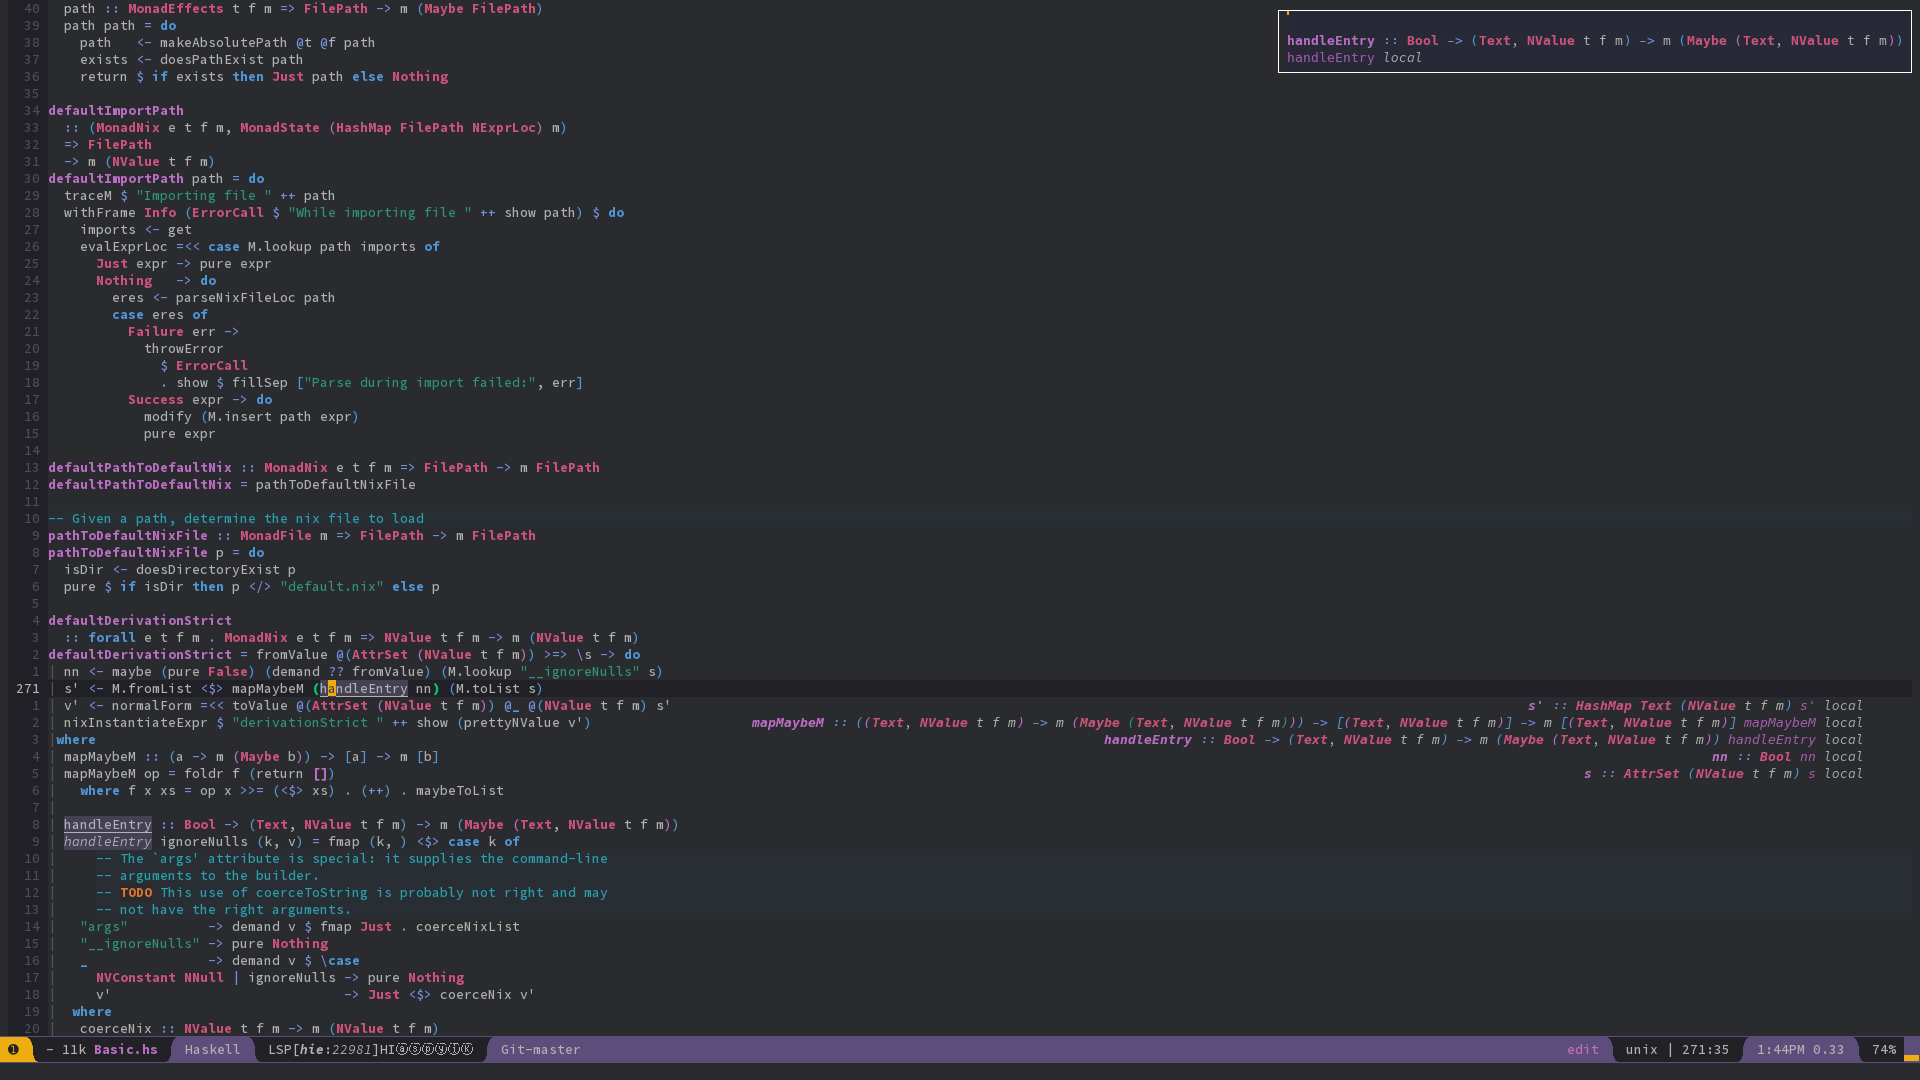
\includegraphics[width=.9\linewidth]{images/Screenshot_20190727_134446.png}
\end{center}

Now, the powers of the Haskell, Nix \& Emacs combined. It's fully in your hands now. Be cautious - you can change the world.

\section{6. (optional) Debugging}
\label{sec:orga2e0684}

\begin{enumerate}
\item If recieving sort-of:
\end{enumerate}

\begin{minted}[]{text}
readCreateProcess : cabal-helper-wrapper failure
\end{minted}

HIE tries to run \texttt{cabal} operations like on the non-Nix system. So it is a problem with detection of \texttt{nix-shell} environment, running inside it.

\begin{enumerate}
\item If HIE keeps getting ready, failing \& restarting - check that the projects \texttt{ghc -{}-version} is declared in your \texttt{all-hie} NixOS configuration.
\end{enumerate}

\chapter{GHC}
\label{sec:orgc98598c}

\section{GHC code check flags}
\label{sec:org2c9198d}

Additional to default settings it is useful to use \texttt{-W}, \texttt{-Wcompat}. \texttt{-Wall} is for purists and would raise noise. They can be supplied in CLI as also in \texttt{.cabal} ghc-option. fr

\texttt{-W} turns on additional useful warnings:
\begin{itemize}
\item \texttt{-Wunused-binds}
\item \texttt{-Wunused-matches}
\item \texttt{-Wunused-foralls}
\item \texttt{-Wunused-imports}
\item \texttt{-Wincomplete-patterns}
\item \texttt{-Wdodgy-exports}
\item \texttt{-Wdodgy-imports}
\item \texttt{-Wunbanged-strict-patterns}
\end{itemize}

\texttt{-Wall} turns on all warnings that indicate potentially suspicious code.

\texttt{-Weverything} turns on all warnings supported by compiler.

\texttt{-Wcompat} turns on warnings that will be enabled by default in the future GHC releases, allows library authors make the code compatible in advance for future GHC releases.

\texttt{-Werror} promotes warnings into fatal \hyperref[org058ef16]{errors}, may be useful for CI runs.

\texttt{-w} turns off all warnings.

\chapter{GHCI}
\label{sec:org859eefc}
\section{Debugging in GHCI}
\label{sec:org1468e86}

Provides:
\begin{itemize}
\item \hyperref[org8140fe5]{set} a breakpoints
\item observe step-by-step \hyperref[org0e2da1f]{evaluation}
\item tracing mode
\end{itemize}

Breakpoints
\begin{minted}[]{text}
:break 2
  :show breaks
  :delete 0
:continue
\end{minted}

Step-by-step
\begin{minted}[]{text}
:step main
\end{minted}

\hyperref[org29c70dc]{List} information at the breakpoint
\begin{minted}[]{text}
:list
\end{minted}

What been evaluated already
\begin{minted}[]{text}
:sprint name
\end{minted}

\chapter{\label{org66a5a82}GHCID}
\label{sec:orga0f5da4}

Commands to run the compile/check loop:

\texttt{cabal} > \texttt{3.0} command:
\begin{minted}[]{fish}
ghcid --command='cabal v2-repl --repl-options=-fno-code --repl-options=-fno-break-on-exception --repl-options=-fno-break-on-error --repl-options=-v1 --repl-options=-ferror-spans --repl-options=-j'
\end{minted}

\texttt{cabal} < \texttt{3.0} command:
\begin{minted}[]{fish}
ghcid --command='cabal new-repl --ghc-options=-fno-code --ghc-options=-fno-break-on-exception --ghc-options=-fno-break-on-error --ghc-options=-v1 --ghc-options=-ferror-spans --ghc-options=-j'
\end{minted}

\texttt{nix-shell} \texttt{cabal} > \texttt{3.0} command:
\begin{minted}[]{fish}
nix-shell --command 'ghcid --command="cabal v2-repl --repl-options=-fno-code --repl-options=-fno-break-on-exception --repl-options=-fno-break-on-error --repl-options=-v1 --repl-options=-ferror-spans --repl-options=-j" '
\end{minted}

\texttt{nix-shell} \texttt{cabal} < \texttt{3.0} command:
\begin{minted}[]{fish}
nix-shell --command 'ghcid --command="cabal new-repl --ghc-options=-fno-code --ghc-options=-fno-break-on-exception --ghc-options=-fno-break-on-error --ghc-options=-v1 --ghc-options=-ferror-spans --ghc-options=-j" '

\end{minted}

\chapter{Continuous integration platrorms (CIs) for Open Source Haskell projets}
\label{sec:org17c5c8d}

Since Open Source projects mostly use free tiers of CIs, and different CIs have different features - there is a \hyperref[org334d524]{constant} flux of how to \hyperref[orgb104f8d]{construct} the best possible integration pipeline for Haskell projects.

The current state of affairs is best put in this quote:
\caption{\href{https://github.com/dhall-lang/dhall-haskell/issues/1678#issuecomment-592960057}{Quote: 2020-02-29: Gabriel Gonzalez about CIs for Haskell Opens Source projects}}
\phantomsection
\label{quote--gonzales-ci}
\begin{quote}
Probably the biggest \hyperref[org24debe5]{constraint} is whether or not CI needs to test Windows or OS X, since build machines for those are harder to come by. We currently use AppVeyor for Windows builds and Travis for OS X builds since they are free. For Linux you can basically use any CI provider, but in this \hyperref[orgf680f86]{case} I pay for a Linode VM which I use to host all Dhall-related infrastructure (i.e. all of the *.dhall-lang.org domains), so I reuse that to host Hydra for Nix-related CI so that I can use more parallelism and more efficient caching to test a wider range of GHC versions on a budget.

For \hyperref[org18d1c17]{testing} OS X and Windows platforms we use \hyperref[org70b1542]{stack}. The main reason we don't use Nix for \hyperref[org752661d]{either} platform is that Nix only supports building release binaries on Linux (and even then it's still experimental).

So the basic summary I can give is:

For \hyperref[org18d1c17]{testing} everything other than cross-platform support: Nix + Linux is best in my opinion

\ldots{} because you get much more control and intelligent build caching, which is usually \hyperref[orgc93f414]{where} most CI solutions fall short

For cross-platform support: \hyperref[org70b1542]{stack} + whatever CI provider provides free builds for that platform

Also, if you ever can pay for your own NixOS VM and you want to reuse the setup I built, you can find the NixOS configuration for dhall-lang.org here:

\url{https://github.com/dhall-lang/dhall-lang/tree/master/nixops}
\end{quote}

\part{Library}
\label{sec:orgc917796}
\chapter{\hyperref[orgf865323]{Exceptions}}
\label{sec:org6b7ece3}

\section{\hyperref[orgf865323]{Exceptions} - optionally \hyperref[org3724659]{pure} extensible \hyperref[orgf865323]{exceptions} that are compatible with the mtl}
\label{sec:orga6fa6bf}
\section{Safe-\hyperref[orgf865323]{exceptions} - safe, simple API \hyperref[orge6d22a9]{equivalent} to the underlying implementation in terms of power, encourages best practices minimizing the chances of getting the \hyperref[org48e9016]{exception} handling wrong.}
\label{sec:orga071c24}
\section{Enclosed-\hyperref[orgf865323]{exceptions} - capture \hyperref[orgf865323]{exceptions} from the enclosed computation, while reacting to asynchronous \hyperref[orgf865323]{exceptions} aimed at the calling thread.}
\label{sec:org582bcf9}

\chapter{Memory management}
\label{sec:orgf2ed2a1}

\section{membrain - \hyperref[org02a9d3a]{type}-safe memory units}
\label{sec:org5a06048}

\chapter{Parsers - megaparsec}
\label{sec:org858521f}

\chapter{CLIs - optparse-\hyperref[org3e108d5]{applicative}}
\label{sec:orgfea6561}

\chapter{HTML - Lucid}
\label{sec:org4d210db}

\chapter{Web applications - Servant}
\label{sec:orgaa098ec}

\chapter{\hyperref[org634b89e]{IO} libraries}
\label{sec:org5df0791}

\section{Conduit - practical, monolythic, guarantees termination return}
\label{sec:orgc88b089}

\section{Pipes + Pipes Parse - modular, more primitive, theoretically driven}
\label{sec:org6e223b0}

\chapter{JSON - aeson}
\label{sec:org31a8f45}

\chapter{\label{orgea6bcd7}Backpack}
\label{sec:org1f2986d}
On 1-st compilation - \emph{*} analyzes the \hyperref[orgdba3c40]{abstract} signatures without loading side modules, doing the \hyperref[orgf45879c]{type check} with assumption that modules provide right \hyperref[org02a9d3a]{type} signatures, the \hyperref[orgd241ff7]{process} does not emitt any \hyperref[orgead9e5b]{binary} code and stores the intermediate code in a special form that allows flexibily connect modules provided. Which allows later to compile project with particular instanciations of the modules. Major work of this \hyperref[orgd241ff7]{process} being done by internal Cabal \emph{*} support and \emph{*} system that modifies the intermediate code to fit the \hyperref[org763755b]{module}.

\part{Draft}
\label{sec:orga8c1941}

\chapter{\hyperref[org48e9016]{Exception} handling}
\label{sec:org67680ad}

\hyperref[orgd241ff7]{Process} of \hyperref[org48e9016]{exception} handling has:
\begin{itemize}
\item raising an \hyperref[org48e9016]{exception}
\item gathering information and handling an \hyperref[org48e9016]{exception}
\item ability to finish important sessions/actions independently of whether \hyperref[org48e9016]{exception} happened or not. That is why it is called guaranteed finalization of important processes.
\end{itemize}

\hyperref[orgf865323]{Exceptions} and their handling are for the boundaries that recieve external things that are not under Haskell control. It is mainly an \hyperref[org634b89e]{IO} handling. The \hyperref[org48e9016]{exception} mechanism may be used for internal \hyperref[org3724659]{pure} Haskell part - if it grew to complex to sort-out some situation try/catch mechanism can be used, but then avoid use of runtime system \hyperref[orgf865323]{exceptions} catch and sort programmically and generally avoid it.

Its better to promote \hyperref[orgf865323]{exceptions} to just checking preconditions.

Wraper with \hyperref[org48e9016]{exception} handler around \hyperref[org0c63459]{function} (\texttt{f}) call means that all untreated \hyperref[org48e9016]{exception} of \hyperref[org0c63459]{function} or its subfunctions would be caught by this wrapper into the \hyperref[org1c2de1b]{scope} \hyperref[orgc93f414]{where} wrapper was used (one syntactic level above \hyperref[org0c63459]{function} \texttt{f}).

\begin{tikzcd}
s \arrow[rd, "Handle/dispatch"'] &                                &                &                                                                            \\
                                 & m \arrow[rd, "Eval \ inside"'] &                &                                                                            \\
                                 &                                & ... \arrow[rd] &                                                                            \\
                                 &                                &                & h \arrow[lluu, "To \ nearest \ exception \ monad"', dotted, bend right=49]
\end{tikzcd}

Any \hyperref[orgc40eb8a]{monad} that short-curcuits after some condition check of first \hyperref[orgb8ce332]{argument} - has \hyperref[org48e9016]{exception} handling potential.

Laziness as \hyperref[orgf865323]{exceptions} are computations - means that some issues would be skipped al togather, in parts that are/were not used would never throw \hyperref[orgf865323]{exceptions}, but also just as computations - \hyperref[orgf865323]{exceptions} would be raised at different times and states during computations.

\hyperref[org48e9016]{Exception} throw breaks \hyperref[orga068b58]{purity}, \hyperref[org0c63459]{function} was called buy returned a result.

Try to raise and resolve all \hyperref[orgf865323]{exceptions} befor aquiring external \hyperref[org634b89e]{IO} resources. And release all resources when or before the exeption can happen.

With concurrency thread could be killed by other threads (that is called to raise an asyncronous \hyperref[org48e9016]{exception} in the thread).

\section{Ideal catching}
\label{sec:org7c39e12}

\begin{itemize}
\item Choose what \hyperref[orgf865323]{exceptions} to catch. Selection depends on the \hyperref[org02a9d3a]{type}.
\item No execution of continuation after throw, only handling.
\item Handle \{,a\}synchronous \hyperref[orgf865323]{exceptions}.
\end{itemize}

\section{\texttt{Control.Exception.Safe} main \hyperref[org61600f0]{sets} of \hyperref[orgfb04cce]{functions}}
\label{sec:org3c75fb6}

\begin{itemize}
\item \texttt{try*} - allows handle \hyperref[org752661d]{Either} returning \hyperref[org05a3981]{types}, bridges the \hyperref[org48e9016]{exception} handling and basic Haskell computation.
\item \texttt{handle*} - describes how to handle \hyperref[org48e9016]{exception} before the \hyperref[orgd1f32d9]{monadic} action itself.
\item \texttt{catch*} - describes how to handle the \hyperref[org48e9016]{exception} after the \hyperref[orgd1f32d9]{monadic} action itself.
\end{itemize}

For asyncronous \hyperref[orgf865323]{exceptions} there are special \hyperref[org0c63459]{function} to catch them: \texttt{catchAsync} and \texttt{handleAsync}.

\texttt{catch} and \texttt{handle} are to catch specific \hyperref[org48e9016]{exception} \hyperref[org02a9d3a]{type}.

\texttt{catches} , \texttt{catchesDeep} and \texttt{catchesAsync} allows to catch matching an elements in the \hyperref[org29c70dc]{list}, and then handle them.

\section{Clean-up of actions/resources}
\label{sec:org68ed0bf}

\begin{itemize}
\item \texttt{bracket*} - computations to aquire and release resource and computation to run in between.
\item \texttt{finally} - allows to run declared computations afterward (even if an \hyperref[org48e9016]{exception} was raised).
\item \texttt{onException} - run computations only if \hyperref[org48e9016]{exception} happened.
\end{itemize}

\section{Ideal model}
\label{sec:org597d8a6}

\begin{itemize}
\item[{$\boxtimes$}] \hyperref[org48e9016]{Exception} must include all \hyperref[org65b79af]{context} information that may be useful.
\item[{$\boxtimes$}] Store information in a form for further probable deeper automatic diagnostic.
\item[{$\boxtimes$}] Sensitive data/dummies for it - can be useful during development.
\item[{$\boxtimes$}] Sensitive data should be stripped from a program logging \& \hyperref[orgf865323]{exceptions}.
\item[{$\boxtimes$}] \hyperref[org48e9016]{Exception} system should be extendable, data storage \& representation should be easily extendable.
\item[{$\boxtimes$}] \hyperref[org48e9016]{Exception} system should allow easy exaustive checking of \hyperref[org058ef16]{errors}, since the different \hyperref[org058ef16]{errors} can happen.
\item[{$\boxtimes$}] \hyperref[org48e9016]{Exception} system should be automatically well-documented and transparent.
\item[{$\boxtimes$}] \hyperref[org48e9016]{Exception} system should have controllable breaking changes downstream.
\item[{$\boxtimes$}] \hyperref[org48e9016]{Exception} system should allow complex composite (\hyperref[org61600f0]{sets}) \hyperref[orgf865323]{exceptions}.
\item[{$\boxtimes$}] \hyperref[org48e9016]{Exception} system should be lightweight on the \hyperref[org02a9d3a]{type} signatures of other \hyperref[orgfb04cce]{functions}.
\item[{$\boxtimes$}] \hyperref[org48e9016]{Exception} system should automate the collection of \hyperref[org65b79af]{context} for a \hyperref[org48e9016]{exception}.
\item[{$\boxtimes$}] \hyperref[org48e9016]{Exception} system should have \hyperref[org88e39a5]{properties} and according \hyperref[orgfb04cce]{functions} for particular \hyperref[org05a3981]{types} of \hyperref[org058ef16]{errors}.
\end{itemize}

\texttt{String} is simple and convinient to throw \hyperref[org48e9016]{exception}, but really a mistake because it the most cumbersome choise:
\begin{itemize}
\item[{$\boxtimes$}] Any \hyperref[org48e9016]{Exception} instance can be converted to a \texttt{String} with \hyperref[org752661d]{either} \texttt{show} or \texttt{displayException.}
\item[{$\square$}] Does not include key debugging information in the \hyperref[org56de0c9]{error} message.
\item[{$\square$}] Does not allow developer to access/manage the \hyperref[org48e9016]{Exception} information.
\item[{$\square$}] \hyperref[org48e9016]{Exception} messages need to be constructed ahead of time, it can not be internationalized, converted to some data/file format.
\item[{$\square$}] \hyperref[org48e9016]{Exception} can have a sensitive information that can be useful for developer during work, but should not be logged/shown to end-user. Stripping it from \texttt{Strings} in the changing project is a hard task.
\item[{$\square$}] Impossible to rely on this representation for further/deeper inspection.
\item[{$\square$}] Impossible to have exhaustive checking - no knowledge no check, no warning if some cases are not handled.
\end{itemize}

\section{Universal \hyperref[org48e9016]{exception} \hyperref[org02a9d3a]{type}}
\label{sec:org3f6b88e}

\begin{itemize}
\item[{$\boxtimes$}] Able to inspect every possible \hyperref[org56de0c9]{error} \hyperref[orgf680f86]{case} with \hyperref[org971a5da]{pattern match}.
\item[{$\boxtimes$}] Self-documenting. Shows the hierarchical system of all \hyperref[orgf865323]{exceptions}.
\item[{$\boxtimes$}] Transparent. Ability to discern in current situation what \hyperref[orgf865323]{exceptions} can happen
\item[{$\square$}] New \hyperref[org48e9016]{exception} \hyperref[org71cf194]{constructor} causes breaking change to downstream.
\item[{$\square$}] Wrongly implies completeness. Untreated \hyperref[org058ef16]{Errors} can happen, different \hyperref[org48e9016]{exception} can arrive from the outside code.
\end{itemize}

Sum \hyperref[org02a9d3a]{type} must be separate, and \hyperref[orga0b5c34]{product type} \hyperref[org750a3dd]{structure} over it.
Separate \hyperref[org48e9016]{exception} \hyperref[org02a9d3a]{type} of 

\section{Individual \hyperref[org48e9016]{exception} \hyperref[org05a3981]{types}}
\label{sec:org4b8844c}

\begin{itemize}
\item[{$\boxtimes$}] Writing \& seing \& working with exactly what will go wrong because there is only one possible \hyperref[org56de0c9]{error} for this \hyperref[org02a9d3a]{type} of \hyperref[org48e9016]{exception}. \hyperref[org971a5da]{Pattern match} happens only onconditions, \hyperref[orgddad11a]{constructors} that should happen.
\item[{$\boxtimes$}] Knowledge what exectly goes wrong allows wide usage of \hyperref[org752661d]{Either}.
\item[{$\square$}] It is hard to handle complex \hyperref[orgf865323]{exceptions} in the unitary system. Real wrorld can return not a particular \hyperref[orgf680f86]{case}, but a \hyperref[org8140fe5]{set} of cases \{\hyperref[org6626401]{object} not found, path is unreachable, access is denied\}.
\item[{$\square$}] \hyperref[org02a9d3a]{Type} signatures grow, and even can become complex, since every \hyperref[orgf680f86]{case} of \hyperref[org48e9016]{exception} has its own \hyperref[org02a9d3a]{type}.
\item[{$\square$}] Impure \texttt{throw} that users can/should use for your code must account for all your \hyperref[org48e9016]{exception} \hyperref[org05a3981]{types}.
\end{itemize}

\section{\hyperref[orgdba3c40]{Abstract} \hyperref[org48e9016]{exception} \hyperref[org02a9d3a]{type}}
\label{sec:org4d9e5fd}

\hyperref[org48e9016]{Exception} \hyperref[org02a9d3a]{type} entirely opague and inspectable only by accessor \hyperref[orgfb04cce]{functions}.
\begin{itemize}
\item[{$\boxtimes$}] Updating the internals without breaking the API
\item[{$\boxtimes$}] Semi-automates the \hyperref[org65b79af]{context} of \hyperref[org48e9016]{exception} with passing it to accessors.
\item[{$\boxtimes$}] Predicates can be \hyperref[org33ef46d]{applied} to more than one \hyperref[org71cf194]{constructor}. Which are \hyperref[org88e39a5]{properties} that allows to make complex \hyperref[orgf865323]{exceptions} much easier to handle.
\item[{$\square$}] Not self-documenting.
\item[{$\square$}] Possible options by design are hidden from the downstream, documentation must be kept.
\item[{$\square$}] When you change the \hyperref[org48e9016]{exception} handling/throwing \hyperref[org058ef16]{errors} it does not shows to the downstream.
\end{itemize}

\section{Composit approach}
\label{sec:org289eb60}

Provide the \hyperref[org8140fe5]{set} of \hyperref[orgddad11a]{constructors} and also a \hyperref[org8140fe5]{set} of predicates and \hyperref[org8140fe5]{set} of accessors.
Use \hyperref[org37a8bc0]{pattern synonyms} to provide a documented accessor \hyperref[org8140fe5]{set} without exposing internal \hyperref[orga6dd88e]{data type}.

\section{The changes in GHC 8.8}
\label{sec:org3a5aed9}

\begin{quote}
The fail method of \hyperref[orgc40eb8a]{Monad} has been removed in favor of the method of the same name in the MonadFail class.

MonadFail(..) is now exported from the Prelude and Control.\hyperref[orgc40eb8a]{Monad} modules.
The MonadFailDesugaring language extension is now deprecated, as its effects are
always enabled.
\end{quote}

So:
\begin{minted}[]{haskell}
import           Control.Monad.Fail
...
class MonadFail m => MonadFile m
...
-- use error instead of fail
Nothing     -> error ("Message " <> show x)
\end{minted}

\section{Diversity in \hyperref[orgf865323]{exceptions}}
\label{sec:org6828552}

\hyperref[org48e9016]{Exception} cause: external or internal.

\hyperref[orgf865323]{Exceptions} used by runtime system

\begin{minted}[]{haskell}
div 1 0
-- *** Exception: divide by zero
\end{minted}

\hyperref[orgf865323]{Exceptions} used by programmers:
\begin{itemize}
\item Language feature
\item Programmable (implemented at library level)
\end{itemize}

\section{\hyperref[org48e9016]{Exception} handling strategies}
\label{sec:org57cd1a4}

\begin{itemize}
\item Ignore
\item Print
\item Repeat
\item Wait, stop, exit
\item Substitute with default
\item Throw
\item Handle
\item Rethrow
\item Emergency exit
\end{itemize}

\section{Asynchronous \hyperref[org48e9016]{exception}}
\label{sec:org979fd10}

\hyperref[orgf865323]{Exceptions} raised as a result of an "external event", such as signal from another thread.

Are raised by \texttt{throwTo}. Are by termin and design should not be catched/handled, by default catching/handling \hyperref[orgfb04cce]{functions} are not catching them, if someone still wants to catch them - there are special \hyperref[org0c63459]{function}: \texttt{catchAsync}.

Further reading: termin and apparatus were introduced by \href{https://www.microsoft.com/en-us/research/wp-content/uploads/2016/07/asynch-exns.pdf}{"Asynchronous Exceptions in Haskell" (Simon Marlow, Simon Peyton Jones, Andrew Moran, John Reppy)}.

\chapter{\hyperref[orgbe0ae3a]{Constraints}}
\label{sec:orgc6268ab}

Very strong Haskell \hyperref[org02a9d3a]{type} system makes possible to work with code from the top down, an \hyperref[org2cd872d]{axiomatic semantics} approach, from \hyperref[orgbe0ae3a]{constraints} into \hyperref[org05a3981]{types}.

\begin{itemize}
\item Helps to form the \hyperref[org40d9bb6]{type level} code (aka \hyperref[org5b585e8]{join} points of the code).
\item Uses the piling up of \hyperref[orgbe0ae3a]{constraints}/\hyperref[org05a3981]{types} information. At some point pick and satisfy \hyperref[orgbe0ae3a]{constraints}, can be done one at a time.
\item Provides hints through \hyperref[org40d9bb6]{type level} formulation for \hyperref[orga267371]{term level} calculations, does not formulate the \hyperref[orga267371]{term level}.
\item Tedious method (a lot of boilerplate and rewriting it) but pretty simple and relaxing.

\item \hyperref[org8140fe5]{Set} of \hyperref[orgbe0ae3a]{constraints}.

\item When it is needed or convenient, single \hyperref[org24debe5]{constraint} gets a little more realistically concrete/abstracted.
\end{itemize}

Main \hyperref[org02a9d3a]{type} detail annotation thread can happen in \texttt{main} or special wrapper \hyperref[org0c63459]{function}, localization is inside \hyperref[orgfb04cce]{functions}.

\begin{enumerate}
\item Rest of \hyperref[orgbe0ae3a]{constraints} \hyperref[org8140fe5]{set} shifts to source \hyperref[org02a9d3a]{type}.
\end{enumerate}

3.a. For the class handled or known how to handle - writte a \hyperref[org9285999]{base case} instance description.

\begin{minted}[]{haskell}
instance (Monad m) => MonadReader r (ReaderT r m)
\end{minted}

3.b. For others write \hyperref[org955a4a1]{recursive} instance descriptions:

All other unsolved \hyperref[orgbe0ae3a]{constraints} move into the source \hyperref[orgea38bb9]{polymorphic} \hyperref[org05f17b5]{variable}.

\begin{minted}[]{haskell}
instance (MonadError e m) => MonadError e (ReaderT r m)
instance (MonadState s m) => MonadState s (ReaderT r m)
\end{minted}

\begin{enumerate}
\item Repeat from 1 until considered done.

\item Code condensed into terse form.
\end{enumerate}

\texttt{MonadError} \hyperref[orgbe0ae3a]{constraints} is \texttt{IOException}, not for the \texttt{String}. \texttt{IOException} vs \texttt{String}.

Reverse pluck \texttt{MonadReader} \hyperref[org24debe5]{constraint} with \texttt{runReader} on the \hyperref[org6626401]{object}.

\texttt{MonadState} - \texttt{StateT}

\chapter{\hyperref[orgc40eb8a]{Monad} transformers and their \hyperref[org3323786]{type classes}}
\label{sec:org1da9b8c}

\chapter{Layering \hyperref[orgc40eb8a]{monad} transformers}
\label{sec:orgb96d37e}

Different layering of the same \hyperref[orgc40eb8a]{monad} transformers is functionality is the same, but the form is different. Surrounding handling \hyperref[orgfb04cce]{functions} would need to be different. 

\chapter{Hoogle}
\label{sec:org8234d7e}

\section{Search}
\label{sec:org3cbc166}

Text search (\hyperref[orgf680f86]{case} insensitive):
\begin{itemize}
\item \texttt{a}
\item \texttt{map}
\item \texttt{con map}
\end{itemize}

\hyperref[org02a9d3a]{Type} search:
\begin{itemize}
\item \texttt{:: a}
\item \texttt{:: a -> a}
\end{itemize}

Text \& \hyperref[org02a9d3a]{type}:
\begin{description}
\item[{=id}] a -> a=
\end{description}

\section{\hyperref[org1c2de1b]{Scope}}
\label{sec:org719e8af}

\subsection{Default}
\label{sec:orge68fc70}

\hyperref[org1c2de1b]{Scope} is \href{http://hackage.haskell.org/platform}{Haskell Platform} (and \href{http://haskell.org/haskellwiki/Keywords}{Haskell keywords)}.

All \href{http://hackage.haskell.org/}{Hackage} packages are available to search with:

\subsection{\hyperref[org012d61d]{Hierarchical module name} system (from big letter):}
\label{sec:org58665b5}

\begin{itemize}
\item \texttt{fold +Data.Map} finds results in the \texttt{Data.Map} \hyperref[org763755b]{module}
\item \texttt{file -System} excludes results from modules such as \texttt{System.IO}, \texttt{System.FilePath.Windows} and \texttt{Distribution.System}
\end{itemize}

\subsection{Packages (lower \hyperref[orgf680f86]{case}):}
\label{sec:org0a46634}
\begin{itemize}
\item \texttt{mode +platform}
\item \texttt{mode +cmdargs} (only)
\item \texttt{mode +platform +cmdargs}
\item \texttt{file -base} (Haskell Platform, excluding the "base" package)
\end{itemize}

\chapter{\label{org1353a91}ST-Trick monad}
\label{sec:orgb1b74a2}

ST is like a \hyperref[org4d22c42]{lexical scope}, \hyperref[orgc93f414]{where} all the \hyperref[org415bea4]{variables}/state disappear when the \hyperref[org0c63459]{function} returns
\url{https://wiki.haskell.ohttps://www.schoolofhaskell.com/school/to-infinity-and-beyond/older-but-still-interesting/deamortized-strg/Monad/ST}
\url{https://dev.to/jvanbruegge/what-the-heck-is-polymorphism-nmh}

\section{\emph{*}}
\label{sec:org2fb303b}

\label{org5e650e1}ST-Trick

\chapter{\label{org752661d}Either}
\label{sec:orgf446b62}

Allows to separate and preserve information about happened, ex. \hyperref[org56de0c9]{error} handling.

\section{\emph{*}}
\label{sec:org92995f3}

\label{org568f474}Either data type

\chapter{\label{orge5f3fa3}Inverse}
\label{sec:org28e44b3}

\begin{enumerate}
\item \hyperref[orgcabcf50]{Inverse function}

\item In logic: \(P \to Q \Rightarrow \neg P \to \neg Q\), \& same for \hyperref[orgea46189]{category duality}.

\item For \hyperref[orgbea159b]{operation}: element that allows reversing \hyperref[orgbea159b]{operation}, having an element that with the \hyperref[org9ed20c5]{dual} produces the \hyperref[org2d14a64]{identity} element.

\item See \hyperref[org069c6f1]{Inversion}.
\end{enumerate}

\chapter{\label{org069c6f1}Inversion}
\label{sec:org9cda45f}

\begin{enumerate}
\item Is a \hyperref[org3ef3428]{permutation} \hyperref[orgc93f414]{where} two elements are out of \hyperref[org23ef0ed]{order}.

\item See \hyperref[orge5f3fa3]{Inverse}
\end{enumerate}

\chapter{\label{orgcabcf50}Inverse function}
\label{sec:org32ef702}

\(f_{x \to y} \circ ({f_{x \to y}})^{-1} = {1}_{x}\)

\emph{*} \(\iff\) \hyperref[org0c63459]{function} is \hyperref[orgf2384e9]{bijective}.
Otherwise - \hyperref[org55b09d9]{partial inverse}

\chapter{\label{orgff9a61a}Inverse morphism}
\label{sec:org35e5766}
For \(f: x \to y\):
\(\exists g \ : \ g \circ f = 1^{x}\) - \(g\) is left \hyperref[orge5f3fa3]{inverse} of \(f\).
\(\exists g \ : \ f \circ g = 1^{y}\) - \(g\) is right \hyperref[orge5f3fa3]{inverse} of \(f\).

\chapter{\label{org55b09d9}Partial inverse}
\label{sec:org533dbcb}

\emph{*} when \hyperref[org0c63459]{function} is now \hyperref[orgf2384e9]{bijective}. When \hyperref[orgf2384e9]{bijective} see \hyperref[orgcabcf50]{inverse function}.

\chapter{\label{org07a8158}PatternSynonyms}
\label{sec:orgb8ca927}
Enables \hyperref[org67f0abd]{pattern synonym} \hyperref[orga3ab72b]{declaration}, which always begins with the \texttt{pattern} word.
Allows to \hyperref[orgdba3c40]{abstract}-away the \hyperref[org23eb7b5]{structures} of pattern matching.

\section{\emph{*}}
\label{sec:org6b212ee}

\label{org67f0abd}Pattern synonym
\label{org37a8bc0}Pattern synonyms

\chapter{\label{org4bb04f8}GHC debug keys}
\label{sec:org93e5062}

\section{\label{org826ec14}-ddump-ds}
\label{sec:org717d040}

Dump desugarer output.

\subsection{\emph{*}}
\label{sec:org53320de}

\label{orgb4b136b}Desugar
\label{orgd72769f}GHC desugar

\chapter{\label{orgb692481}GHC optimize keys}
\label{sec:orgff88de9}

\section{\label{org9f28644}-foptimal-applicative-do}
\label{sec:orgeeb0580}

\(O(n^3)\)
Always finds optimal \hyperref[org9f4608a]{reduction} into <*> for \hyperref[org3cb8128]{ApplicativeDo} do notation.

\chapter{\label{org6fc8d68}Computational trinitarianism}
\label{sec:org316b36d}

Taken from: \url{https://ncatlab.org/nlab/show/computational+trinitarianism}

Under the \hyperref[orgde5d369]{statements}:

\begin{itemize}
\item \hyperref[org2f362e9]{propositions} as \hyperref[org05a3981]{types}

\item programs as proofs

\item \hyperref[orgf43c12d]{relation} between \hyperref[org02a9d3a]{type} theory and \hyperref[org77a2b71]{category} theory
\end{itemize}

the following notions are \hyperref[orge6d22a9]{equivalent}:

== \hyperref[org6df087c]{proposition} proof (Logic)

== generalized element of an \hyperref[org6626401]{object} (\hyperref[org77a2b71]{Category} theory)

== typed program with output (\hyperref[org02a9d3a]{Type} theory \& Computer science)

\begin{sidewaystable}[htbp]
\caption{\label{tab--computational-trinitarianism}\hyperref[org6fc8d68]{Computational trinitarianism}}
\centering
\begin{tabu} spread \linewidth {lll}
\toprule
\href{https://ncatlab.org/nlab/show/logic}{Logic} & \href{https://ncatlab.org/nlab/show/category+theory}{Category theory} & \href{https://ncatlab.org/nlab/show/type+theory}{Type theory}\\
\midrule
\href{https://ncatlab.org/nlab/show/true}{true} & \href{https://ncatlab.org/nlab/show/terminal+object}{terminal object}/\href{https://ncatlab.org/nlab/show/\%28-2\%29-truncated+object}{(-2)-truncated object} & \href{https://ncatlab.org/nlab/show/h-level+0}{h-level 0}-\href{https://ncatlab.org/nlab/show/type}{type}/\href{https://ncatlab.org/nlab/show/unit+type}{unit type}\\
\href{https://ncatlab.org/nlab/show/false}{false} & \href{https://ncatlab.org/nlab/show/initial+object}{initial object} & \href{https://ncatlab.org/nlab/show/empty+type}{empty type}\\
\href{https://ncatlab.org/nlab/show/proposition}{proposition} & \href{https://ncatlab.org/nlab/show/\%28-1\%29-truncated+object}{(-1)-truncated object} & \href{https://ncatlab.org/nlab/show/h-proposition}{h-proposition}, \href{https://ncatlab.org/nlab/show/mere+proposition}{mere proposition}\\
\href{https://ncatlab.org/nlab/show/proof}{proof} & \href{https://ncatlab.org/nlab/show/generalized+element}{generalized element} & \href{https://ncatlab.org/nlab/show/program}{program}\\
\href{https://ncatlab.org/nlab/show/cut+rule}{cut rule} & \href{https://ncatlab.org/nlab/show/composition}{composition} of \href{https://ncatlab.org/nlab/show/classifying+morphisms}{classifying morphisms} / \href{https://ncatlab.org/nlab/show/pullback}{pullback} of \href{https://ncatlab.org/nlab/show/display+maps}{display maps} & \href{https://ncatlab.org/nlab/show/substitution}{substitution}\\
\href{https://ncatlab.org/nlab/show/cut+elimination}{cut elimination} for \href{https://ncatlab.org/nlab/show/implication}{implication} & \href{https://ncatlab.org/nlab/show/counit}{counit} for hom-\hyperref[org939b1cc]{tensor} adjunction & \href{https://ncatlab.org/nlab/show/beta+reduction}{beta reduction}\\
introduction rule for \href{https://ncatlab.org/nlab/show/implication}{implication} & \href{https://ncatlab.org/nlab/show/unit}{unit} for hom-\hyperref[org939b1cc]{tensor} adjunction & \href{https://ncatlab.org/nlab/show/eta+conversion}{eta conversion}\\
\href{https://ncatlab.org/nlab/show/logical+conjunction}{logical conjunction} & \href{https://ncatlab.org/nlab/show/product}{product} & \href{https://ncatlab.org/nlab/show/product+type}{product type}\\
\href{https://ncatlab.org/nlab/show/disjunction}{disjunction} & \href{https://ncatlab.org/nlab/show/coproduct}{coproduct} (\href{https://ncatlab.org/nlab/show/\%28-1\%29-truncation}{(-1)-truncation} of) & \href{https://ncatlab.org/nlab/show/sum+type}{sum type} (\href{https://ncatlab.org/nlab/show/bracket+type}{bracket type} of)\\
\href{https://ncatlab.org/nlab/show/implication}{implication} & \href{https://ncatlab.org/nlab/show/internal+hom}{internal hom} & \href{https://ncatlab.org/nlab/show/function+type}{function type}\\
\href{https://ncatlab.org/nlab/show/negation}{negation} & \href{https://ncatlab.org/nlab/show/internal+hom}{internal hom} into \href{https://ncatlab.org/nlab/show/initial+object}{initial object} & \href{https://ncatlab.org/nlab/show/function+type}{function type} into \href{https://ncatlab.org/nlab/show/empty+type}{empty type}\\
\href{https://ncatlab.org/nlab/show/universal+quantification}{universal quantification} & \href{https://ncatlab.org/nlab/show/dependent+product}{dependent product} & \href{https://ncatlab.org/nlab/show/dependent+product+type}{dependent product type}\\
\href{https://ncatlab.org/nlab/show/existential+quantification}{existential quantification} & \href{https://ncatlab.org/nlab/show/dependent+sum}{dependent sum} (\href{https://ncatlab.org/nlab/show/\%28-1\%29-truncation}{(-1)-truncation} of) & \href{https://ncatlab.org/nlab/show/dependent+sum+type}{dependent sum type} (\href{https://ncatlab.org/nlab/show/bracket+type}{bracket type} of)\\
\href{https://ncatlab.org/nlab/show/equivalence}{equivalence} & \href{https://ncatlab.org/nlab/show/path+space+object}{path space object} & \href{https://ncatlab.org/nlab/show/identity+type}{identity type}\\
\href{https://ncatlab.org/nlab/show/equivalence+class}{equivalence class} & \href{https://ncatlab.org/nlab/show/quotient}{quotient} & \href{https://ncatlab.org/nlab/show/quotient+type}{quotient type}\\
\href{https://ncatlab.org/nlab/show/induction}{induction} & \href{https://ncatlab.org/nlab/show/colimit}{colimit} & \href{https://ncatlab.org/nlab/show/inductive+type}{inductive type}, \href{https://ncatlab.org/nlab/show/W-type}{W-type}, \href{https://ncatlab.org/nlab/show/M-type}{M-type}\\
higher \href{https://ncatlab.org/nlab/show/induction}{induction} & \href{https://ncatlab.org/nlab/show/\%28infinity\%2C1\%29-colimit}{higher colimit} & \href{https://ncatlab.org/nlab/show/higher+inductive+type}{higher inductive type}\\
\href{https://ncatlab.org/nlab/show/completely+presented+set}{completely presented set} & \href{https://ncatlab.org/nlab/show/discrete+object}{discrete object}/\href{https://ncatlab.org/nlab/show/0-truncated+object}{0-truncated object} & \href{https://ncatlab.org/nlab/show/h-level+2}{h-level 2}-\href{https://ncatlab.org/nlab/show/type}{type}/\href{https://ncatlab.org/nlab/show/preset}{preset}/\href{https://ncatlab.org/nlab/show/h-set}{h-set}\\
\href{https://ncatlab.org/nlab/show/set}{set} & \href{https://ncatlab.org/nlab/show/groupoid+object+in+an+\%28infinity\%2C1\%29-category}{internal 0-groupoid} & \href{https://ncatlab.org/nlab/show/Bishop+set}{Bishop set}/\href{https://ncatlab.org/nlab/show/setoid}{setoid}\\
\href{https://ncatlab.org/nlab/show/universe}{universe} & \href{https://ncatlab.org/nlab/show/object+classifier}{object classifier} & \href{https://ncatlab.org/nlab/show/type+of+types}{type of types}\\
\href{https://ncatlab.org/nlab/show/modality}{modality} & \href{https://ncatlab.org/nlab/show/closure+operator}{closure operator}, (\href{https://ncatlab.org/nlab/show/idempotent+monad}{idemponent}) \href{https://ncatlab.org/nlab/show/monad}{monad} & \href{https://ncatlab.org/nlab/show/modal+type+theory}{modal type theory}, \href{https://ncatlab.org/nlab/show/monad+\%28in+computer+science\%29}{monad (in computer science)}\\
\href{https://ncatlab.org/nlab/show/linear+logic}{linear logic} & (\href{https://ncatlab.org/nlab/show/symmetric+monoidal+category}{symmetric}, \href{https://ncatlab.org/nlab/show/closed+monoidal+category}{closed}) \href{https://ncatlab.org/nlab/show/monoidal+category}{monoidal category} & \href{https://ncatlab.org/nlab/show/linear+type+theory}{linear type theory}/\href{https://ncatlab.org/nlab/show/quantum+computation}{quantum computation}\\
\href{https://ncatlab.org/nlab/show/proof+net}{proof net} & \href{https://ncatlab.org/nlab/show/string+diagram}{string diagram} & \href{https://ncatlab.org/nlab/show/quantum+circuit}{quantum circuit}\\
(absence of) \href{https://ncatlab.org/nlab/show/contraction+rule}{contraction rule} & (absence of) \href{https://ncatlab.org/nlab/show/diagonal}{diagonal} & \href{https://ncatlab.org/nlab/show/no-cloning+theorem}{no-cloning theorem}\\
 & \href{https://ncatlab.org/nlab/show/synthetic+mathematics}{synthetic mathematics} & \href{https://ncatlab.org/nlab/show/domain+specific+embedded+programming+language}{domain specific embedded programming language}\\
\bottomrule
\end{tabu}
\end{sidewaystable}

\section{\emph{*}}
\label{sec:org9ddeec3}
\label{org6b613be}Trinitarism

\chapter{Techniques functional programming deals with the state}
\label{sec:org539d3b5}

\section{Minimizing}
\label{sec:org4740bf2}

Do not rely on state, try not to change the state. Use it only when it is very necessary.

\section{Concentrating}
\label{sec:org2dfdc20}

Concentrate the state in one place.

\section{Deferring}
\label{sec:org8b5ebbd}

Defer state to the last step of the program, or to external system.

\chapter{\hyperref[orgd1f32d9]{Monadic} \hyperref[org56de0c9]{Error} handling}
\label{sec:org6b2e25b}

\begin{minted}[]{haskell}
(>>=) :: m a -> (a -> m b) -> m b -- λA.E ∨ A - computes and drops if error value happens.
catch :: c a -> (e -> c a) -> c a -- λE.E ∨ A - handles "errors" as "normal" values and stops when an "error" is finally handled.
\end{minted}

\chapter{\hyperref[orgfb04cce]{Functions}}
\label{sec:org80e1262}

Total \hyperref[org0c63459]{function} uses \hyperref[org66948b1]{domain} fully, but takes only part of the \hyperref[org088b04d]{codomain}.
\hyperref[org0c63459]{Function} allows to collapse \hyperref[org66948b1]{domain} values into \hyperref[org088b04d]{codomain} value. Meaning the \hyperref[org0c63459]{function} allows to loose the information.
So total \hyperref[org0c63459]{function} is a computation that looses the information or into bigger codomains.
That is why the \hyperref[org0c63459]{function} has a directionality, and \hyperref[orge5f3fa3]{inverse} total \hyperref[orgd241ff7]{process} is partially possible.

Directionality and invertability are terms.

\chapter{\label{orgf5d32f1}Void}
\label{sec:org523bb1f}

Emptiness.

Can not be grasped, touched.

A logically uninhabited \hyperref[orga6dd88e]{data type}.

(Since \hyperref[orgc7a3ca3]{basis} of logic is tautologically True and \hyperref[orgf5d32f1]{Void} value can not be addressed - there is a logical paradox with the \hyperref[orgf5d32f1]{Void}).

Is an \hyperref[org6626401]{object} includded into the \hyperref[org19590fc]{Hask} \hyperref[org77a2b71]{category}, since:
\begin{minted}[]{haskell}
:t (id :: Void -> Void)
(id :: Void -> Void) :: Void -> Void
\end{minted}

\texttt{id} for it exists.

\hyperref[org02a9d3a]{Type} system corresponds to \hyperref[org6a3d19c]{constructive logic} and not to the classical logic.
Classical logic answers the question "Is this actually true".
Constuctive (Intuitionistic) logic answers the question "Is this provable".

Also has \hyperref[orgfb04cce]{functions}:
\begin{minted}[]{haskell}
-- Represents logical principle of explosion: from falsehood, anything follows.
absurd :: Void -> a

-- If Functor holds only Void - it holds no values.
vacuous :: Functor f => f Void -> f a

-- If Monad holds only Void - it holds no values.
vacuousM :: Monad m => m Void -> m a
\end{minted}

Design pattern: use \hyperref[orgea38bb9]{polymorphic} \hyperref[org7d7f5e3]{data types} and \hyperref[orgf5d32f1]{Void} to get rid of possibilities when you need to.

\section{\emph{*}}
\label{sec:orgcfa07f7}
\label{org87646f9}Nothing, Haskell \hyperref[org4d65c6e]{expressions} can't return \hyperref[orgf5d32f1]{Void}.

Also see: \hyperref[org2687b3e]{Maybe}.

\chapter{Constructive proof}
\label{sec:orgcefbf1c}

Method of proof that demonstrates the existence of a mathematical \hyperref[org6626401]{object} by creating or providing a method for creating the \hyperref[org6626401]{object}.

\chapter{Intuitionistic logic}
\label{sec:org7a2595a}

\hyperref[org6df087c]{Proposition} considered \texttt{True} due to direct evidence of existence through constructive proof using \hyperref[orgfe74e9f]{Curry}-Howard \hyperref[orged5fbaf]{isomorphism}.

\emph{*} does not include classic logic fundamental axioms of the excluded middle and double negation elimination. Hense \emph{*} is weaker then classical logic. Classical logic includes \emph{*}, all theorems of \emph{*} are also in classical logic.

\section{\emph{*}}
\label{sec:org2225313}

\label{org6a3d19c}Constructive logic

\chapter{\label{orgeedd0f0}Principle of explosion}
\label{sec:org2fbb5c8}
If asserted \hyperref[orgb39efd8]{statement} contains some \hyperref[org56de0c9]{error} or contradiction - anything can be proven trough it.
The more there is an \hyperref[org56de0c9]{error} - the easier logic chain arrives at any target.

Ancient principle of logic. Both in classical \& intuitionistic logic.

\section{\emph{*}}
\label{sec:org609cd49}

\label{org019a471}Ex falso quodlibet
\label{org66bd6a8}Ex falso sequitur quodlibet
\label{orga443786}EFG
\label{orgd2ed192}Ex contradictione quodlibet
\label{org503425a}Ex contradictione sequitur quodlibet
\label{org9ea5631}ECQ
\label{org33338b9}Deductive explosion
\label{orgedfa0fb}Pseudo-Scotus

\chapter{Universal \hyperref[orgb96cce5]{property}}
\label{sec:org95cfc8e}

A \hyperref[orgb96cce5]{property} of some construction which boils down to (is manifestly \hyperref[orge6d22a9]{equivalent} to) the \hyperref[orgb96cce5]{property} that an associated \hyperref[org6626401]{object} is a universal \hyperref[orge742ac7]{initial object} of some (auxiliary) \hyperref[org77a2b71]{category}.

\chapter{Yoneda lemma}
\label{sec:org5ecb6b6}

Allows the embedding of any \hyperref[org77a2b71]{category} into a \hyperref[org77a2b71]{category} of \hyperref[org880fb2b]{functors} (\hyperref[org23504df]{contravariant} \hyperref[org8140fe5]{set}-valued \hyperref[org880fb2b]{functors}) defined on that \hyperref[org77a2b71]{category}. It also clarifies how the embedded \hyperref[org77a2b71]{category}, of representable \hyperref[org880fb2b]{functors} and their \hyperref[org7610ded]{natural transformations}, relates to the other \hyperref[orgbc3544a]{objects} in the larger \hyperref[org41edcd3]{functor} \hyperref[org77a2b71]{category}.

The Yoneda lemma suggests that instead of studying the (locally small) \hyperref[org77a2b71]{category} C \{\displaystyle \{\mathcal \{C\}\}\} \mathcal{C} , one should study the \hyperref[org77a2b71]{category} of all \hyperref[org880fb2b]{functors} of C \{\displaystyle \{\mathcal \{C\}\}\} \mathcal{C} into S e t \{\displaystyle \mathbf \{\hyperref[org8140fe5]{Set}\} \} \mathbf{Set} (the \hyperref[org77a2b71]{category} of \hyperref[org61600f0]{sets} with \hyperref[orgfb04cce]{functions} as \hyperref[orgd74c740]{morphisms}). S e t \{\displaystyle \mathbf \{\hyperref[org8140fe5]{Set}\} \} \mathbf{Set} is a \hyperref[org77a2b71]{category} we think we understand well, and a \hyperref[org41edcd3]{functor} of C \{\displaystyle \{\mathcal \{C\}\}\} \mathcal{C} into S e t \{\displaystyle \mathbf \{\hyperref[org8140fe5]{Set}\} \} \mathbf{Set} can be seen as a "representation" of C \{\displaystyle \{\mathcal \{C\}\}\} \mathcal{C} in terms of known \hyperref[org23eb7b5]{structures}. The original \hyperref[org77a2b71]{category} C \{\displaystyle \{\mathcal \{C\}\}\} \mathcal{C} is contained in this \hyperref[org41edcd3]{functor} \hyperref[org77a2b71]{category}, but new \hyperref[orgbc3544a]{objects} appear in the \hyperref[org41edcd3]{functor} \hyperref[org77a2b71]{category}, which were absent and "hidden" in C \{\displaystyle \{\mathcal \{C\}\}\} \mathcal{C} . Treating these new \hyperref[orgbc3544a]{objects} just like the old ones often unifies and simplifies the theory.

\chapter{\hyperref[orgbb05502]{Monoidal} \hyperref[org77a2b71]{category}, functoriality of ADTs, Profunctors}
\label{sec:orgcbb4a2c}

\hyperref[org77a2b71]{Category} equipped with \hyperref[org064d387]{tensor product}.
\begin{minted}[]{haskell}
<>
\end{minted}
wich is a \hyperref[org41edcd3]{functor} for \emph{*}.

\hyperref[org8140fe5]{Set} \hyperref[org77a2b71]{category} can be \hyperref[orgbb05502]{monoidal} under both \hyperref[org031d37b]{product} (having \hyperref[org03474e7]{terminal object}) or \hyperref[orgfa2684b]{coproduct} (having \hyperref[orge742ac7]{initial object}) operations, if according \hyperref[orgbea159b]{operation} exist for all \hyperref[orgbc3544a]{objects}.

Any one-\hyperref[org6626401]{object} \hyperref[org77a2b71]{category} is \emph{*}.

\((a, ()) \sim a\) up to unique \hyperref[orged5fbaf]{isomorphism}, which is called \hyperref[org7cf79be]{Lax} \hyperref[orgbb05502]{monoidal} \hyperref[org41edcd3]{functor}.

\hyperref[org031d37b]{Product} and \hyperref[orgfa2684b]{coproduct} are \hyperref[org36321e4]{functorial}, so, since:
\hyperref[org673cfcb]{Algebraic data type} construction can use:
\begin{itemize}
\item \hyperref[org7224d29]{Type constructor}
\item \hyperref[orgbcce9b9]{Data constructor}
\item \hyperref[org3d0f9c4]{Const functor}
\item \hyperref[org2d14a64]{Identity} \hyperref[org41edcd3]{functor}
\item \hyperref[org031d37b]{Product}
\item \hyperref[orgfa2684b]{Coproduct}
\end{itemize}

Any \hyperref[org673cfcb]{algebraic data type} is \hyperref[org36321e4]{functorial}.

\chapter{\label{org3d0f9c4}Const functor}
\label{sec:org554c07b}

Maps all \hyperref[orgbc3544a]{objects} of source \hyperref[org77a2b71]{category} into one (fixed) \hyperref[org6626401]{object} of target \hyperref[org77a2b71]{category}, and all \hyperref[orgd74c740]{morphisms} to \hyperref[org2d14a64]{identity} \hyperref[orgb72212b]{morphism} of that fixed \hyperref[org6626401]{object}.

\begin{minted}[]{haskell}
instance Functor (Const c)
 where
  fmap :: (a -> b) -> Const c a -> Const c b
  fmap _ (Const c) = Const c
\end{minted}

In \hyperref[org77a2b71]{Category} theory denoted:
\begin{minted}[]{text}
Δ
\end{minted}

Last \hyperref[org02a9d3a]{type} \hyperref[orgd1897e3]{parameter} that bears the target \hyperref[org02a9d3a]{type} of lifted \hyperref[org0c63459]{function} (\texttt{b}) and is a \hyperref[orge1f6947]{proxy type}.

Analogy: the container that allways has an \hyperref[org6626401]{object} attached to it, and everything that is put inside - changes the container \hyperref[org02a9d3a]{type} accordingly, and dissapears.

\chapter{\label{org1bed8db}Arrow in Haskell}
\label{sec:orgbdb485f}

\begin{minted}[]{haskell}
(->) a b = a -> b
\end{minted}
\hyperref[org36321e4]{Functorial} in the last \hyperref[orgb8ce332]{argument} \& called Reader \hyperref[org41edcd3]{functor}.

\begin{minted}[]{haskell}
newtype Reader c a = Reader (c -> a)

  fmap = ( . )
\end{minted}

\chapter{\hyperref[org47a0dbf]{Contravariant functor}}
\label{sec:org095de17}

\begin{minted}[]{haskell}
fmap :: (a -> b) -> Op c a -> Op c b
                (a -> c) -> (b -> c)
\end{minted}

\begin{tikzcd}
a \arrow[r] \arrow[rd] & b \arrow[d, dashed] \\
                       & c
\end{tikzcd}

\((a \to b)^{C} = (a \leftarrow b)^{C^{op}}\)

\begin{minted}[]{haskell}
class Contravariant f
 where
  contramap :: (b -> a) -> (f a -> f b)
\end{minted}

\begin{tikzcd}
a \arrow[r] \arrow[rd] & b \arrow[d, "contravariant", dashed] \\
                       & c
\end{tikzcd}

If \hyperref[org99c4ebc]{arrows} does not commute Contravatiant funtor anyway allows to \hyperref[orgb104f8d]{construct} transformation between these such \hyperref[org99c4ebc]{arrows} to other \hyperref[orgf10b1c8]{arrow}.

\chapter{Profunctor}
\label{sec:org10e3927}

\begin{minted}[]{haskell}
(->) a b
\end{minted}

\(C^{op} \times C \to C\)

It is called profunctor.

\begin{minted}[]{haskell}
dimap :: (a' -> a) -> (b -> b') -> p a b -> p a' b'
\end{minted}

So, profunctor in \hyperref[orgf680f86]{case} of \hyperref[orgf10b1c8]{arrow}:

\begin{tikzcd}
a \arrow[dd, "h"] &  & a' \arrow[ll, "f"] \arrow[dd, "profunctor", dashed] \\
                  &  &                                                     \\
b \arrow[rr, "g"] &  & b'
\end{tikzcd}

\begin{minted}[]{haskell}
dimap :: (a' -> a) -> (b -> b') -> p a b -> p a' b'
dimap ::    f          g     -> (a -> b) -> (a' -> b') 
dimap ::    f          g     ->    h    -> (a' -> b')
dimap = g . h . f
\end{minted}

It is \hyperref[org47a0dbf]{contravariant functor} in the first \hyperref[orgb8ce332]{argument}, and \hyperref[orgc03a723]{covariant functor} in the second \hyperref[orgb8ce332]{argument}.

\begin{minted}[]{haskell}
dimap id <==> fmap
(flip dimap) id <==> contramap
\end{minted}

\chapter{Coerce}
\label{sec:org6057b72}

Operates under condition that source and target \hyperref[org05a3981]{types} have same representation.
Same representation means they are \hyperref[org02a9d3a]{type} aliases, or it the compiler can \hyperref[org2f48046]{infer} that they have the same representation. 
Directly shares the values from the source \hyperref[org02a9d3a]{type} to the target \hyperref[org02a9d3a]{type}.
Conversion is free, there is no run-time computations.

The \hyperref[org0c63459]{function} implementing the transition:
\begin{minted}[]{haskell}
coerce :: Coercible a b => a -> b
\end{minted}

\hyperref[org639e5cc]{Type class} implementing the instances for transitions:
\begin{minted}[]{haskell}
class a ~R# b => Coercible (a :: k0) (b :: k0)
\end{minted}
When compiler detects \hyperref[org05a3981]{types} have same \hyperref[org750a3dd]{structure}, \hyperref[org639e5cc]{type class} instances coerse implementation for this pairs of \hyperref[org05a3981]{types}. This \hyperref[org639e5cc]{type class} does not have regular instances; instead they are created on-the-fly during \hyperref[org02a9d3a]{type}-checking. Trying to manually declare an instance of Coercible is an \hyperref[org56de0c9]{error}.

\section{\emph{*}}
\label{sec:org359a78f}

Coercible

\chapter{Universal/Existential \hyperref[orgf85457f]{quantification}}
\label{sec:org4d33977}

\(\forall\) Universal \hyperref[org7aeeefd]{quantifier} - a general solution.
\(\exists\) Existential \hyperref[org7aeeefd]{quantifier} - a \hyperref[orgfbd6df6]{local} solution.

Haskell existentials are always result in throwing aways \hyperref[org02a9d3a]{type} information.

Useful to be able to work with data from at external world that we do not know definite \hyperref[org02a9d3a]{type} at compile time.

Some information about existentially \hyperref[orgf00d307]{quantified} \hyperref[org02a9d3a]{type} should be preserved to ba able to transrofm it.



Additional reading: \url{https://markkarpov.com/post/existential-quantification.html}

\part{Reference}
\label{sec:org4981fa6}

\chapter{\label{org1871468}Functor-Applicative-Monad Proposal}
\label{sec:org3a079cf}
Well known event in Haskell history: \url{https://github.com/quchen/articles/blob/master/applicative\_monad.md}.

Math justice was restored with a RETroactive CONtinuity. Invented in computer science term \hyperref[org3e108d5]{Applicative} (\hyperref[org7cf79be]{lax} \hyperref[orgbb05502]{monoidal} \hyperref[org41edcd3]{functor}) become a \hyperref[orgdbf03a7]{superclass} of \hyperref[orgc40eb8a]{Monad}.

\& that is why:
\begin{itemize}
\item \texttt{return = pure}
\item \texttt{ap = <*>}
\item \texttt{>> = *>}
\item \texttt{liftM = liftA = fmap}
\item \texttt{liftM* = liftA*}
\end{itemize}

Also, a side-kick - \hyperref[orgeb027e4]{Alternative} became a \hyperref[orgdbf03a7]{superclass} of \hyperref[org1fa170e]{MonadPlus}. Hense:
\begin{itemize}
\item \texttt{mzero = empty}
\item \texttt{mplus = (<|>)}
\end{itemize}

Work of unification continues under: \url{https://gitlab.haskell.org/ghc/ghc/wikis/proposal/monad-of-no-return}

\section{\emph{*}}
\label{sec:orgf7d4b13}

\label{org692dc22}Applicative-Monad proposal
\label{org5c03ec6}AMP

\chapter{Haskell-98}
\label{sec:orge774afc}

\section{\label{org68cab07}Old instance termination rules}
\label{sec:org1835869}

\begin{enumerate}
\item \(\forall\) class \hyperref[org24debe5]{constraint} (C t1 .. tn):
1.1. \hyperref[org02a9d3a]{type} \hyperref[org415bea4]{variables} have occurances \(\le\) head
1.2. \hyperref[orgddad11a]{constructors}+\hyperref[org415bea4]{variables}+repetitions < head
1.3. \textlnot{} \hyperref[org02a9d3a]{type} \hyperref[orgfb04cce]{functions} (\hyperref[org02a9d3a]{type} func \hyperref[org27ce4ae]{application} can expand to \hyperref[orgcc5605e]{arbitrary} size)
\item \(\forall\) \hyperref[org9e2fa1f]{functional dependencies}, ⟨tvs⟩\textsubscript{left} \(\to\) ⟨tvs⟩\textsubscript{right}, of the class, every \hyperref[org2833214]{type variable} in S(⟨tvs⟩\textsubscript{right}) must appear in S(⟨tvs⟩\textsubscript{left}), \hyperref[orgc93f414]{where} S is the substitution mapping each \hyperref[org2833214]{type variable} in the class \hyperref[orga3ab72b]{declaration} to the corresponding \hyperref[org02a9d3a]{type} in the instance head.
\end{enumerate}

\chapter{Performance results and comparisons of \hyperref[org05a3981]{types} \& solutions}
\label{sec:orgaada5fa}
\href{https://github.com/haskell-perf}{Haskell performance}

\chapter{Literature}
\label{sec:orgc0944c1}

\begin{itemize}
\item "GHC User’s Guide Documentation" (GHC Team): \href{https://downloads.haskell.org/\~ghc/latest/docs/users\_guide.pdf}{PDF}
\item "What I Wish I Knew When Learning Haskell" (Stephen Diehl \& contributors): \href{http://dev.stephendiehl.com/hask/tutorial.pdf}{PDF}
\item "\hyperref[org77a2b71]{Category} Theory for Programmers" (Bartosz Milewski \& contributors): \href{https://s3.amazonaws.com/milewski-ctfp-pdf/category-theory-for-programmers.pdf}{PDF}
\end{itemize}

\part{Giving back}
\label{sec:org6795e8f}

\textgreek{λειτ}       <- \textgreek{λαός}  \emph{Laos}       the people
    \textgreek{ουργός} <- \textgreek{ἔργο}  \emph{ergon}             work
\textgreek{λειτουργία}          \emph{leitourgia} public work

Moral value of people developed from the community to give back, improving the community.

The life is beautiful.
For all humans that make the life have more magic.

This study and work would not be possible without the community: tearchers, mathematicians, Haskellers, scientists, creators, contributors. These sides of people are fascinating.


Special accolades for the guys at Serokell. They were the force that got me inspired \& gave resources to seriously learn Haskell and create this pocket guide.
\end{document}
